\documentclass{umthesis}          % for Ph.D. dissertation or proposal

\usepackage{graphicx}
\usepackage{epsfig}
\usepackage{amssymb}
\usepackage{amsfonts}
\usepackage{verbatim}
\usepackage{moreverb}
\usepackage{cancel}
\usepackage{fancyhdr}
\usepackage{algorithmic}
\usepackage[algosection,lined,linesnumbered,ruled]{algorithm2e}
%\usepackage[algochapter,lined,linesnumbered,ruled]{algorithm2e}
\usepackage{epstopdf}
\usepackage{amssymb,amsfonts,amsmath,amsthm}
\usepackage{subfigure}

\usepackage{rotating}
\usepackage{framed}
\usepackage{xcolor}
\usepackage{soul}
\usepackage{fancyhdr}
\usepackage{enumerate}
\usepackage{cancel}
\usepackage{endnotes}
\usepackage{datetime}
\usepackage{hyperref}  %does not compile when using this line


\newtheorem{theorem}{Theorem}[chapter]
%\setcounter{theorem}{0}
\newtheorem{claim}[theorem]{Claim}
\newtheorem{conjecture}[theorem]{Conjecture}
\newtheorem{corollary}[theorem]{Corollary}
\newtheorem{fact}[theorem]{Fact}
\newtheorem{lemma}[theorem]{Lemma}
\newtheorem{meta-proposition}[theorem]{Meta-Proposition}
\newtheorem{note}[theorem]{Note}
\newtheorem{observation}[theorem]{Observation}
\newtheorem{proposition}[theorem]{Proposition}
\newtheorem{proviso}[theorem]{Proviso}         
\newtheorem{question}[theorem]{Question}         
\newtheorem{remark}[theorem]{Remark}         
\newtheorem{define}{Definition}     


%%%%%%%%%%%%%%%  ROLLBACK MACROS  %%%%%%%%%%%%%%%%%%%%%%%%%%%%%%%%%%%%%%%%
\newcommand{\minv}{$\overrightarrow{min}$ }
\newcommand{\minvi}{$\overrightarrow{min}_i$ }
\newcommand{\minvis}{$\overrightarrow{min}_i$}
\newcommand{\minvj}{$\overrightarrow{min}_j$ }
\newcommand{\minvjs}{$\overrightarrow{min}_j$}
\newcommand{\minvv}{$\overrightarrow{min}_v$ }
\newcommand{\minvvs}{$\overrightarrow{min}_v$}
\newcommand{\dmatrix}{$dmatrix$ }
\newcommand{\dmatrixs}{$dmatrix$}
\newcommand{\dmatrixi}{$dmatrix_i$ }
\newcommand{\dmatrixis}{$dmatrix_i$} 
\newcommand{\dmatrixj}{$dmatrix_j$ }
\newcommand{\dmatrixjs}{$dmatrix_j$} 
\newcommand{\dmatrixv}{$dmatrix_v$ }
\newcommand{\dmatrixvs}{$dmatrix_v$} 
\newcommand{\dv}{{DV$^+$ }}
\newcommand{\Bad}{{$\overline{V}$ }}
\newcommand{\Bads}{{$\overline{V}$}}
\newcommand{\bad}{{$\overline{v}$ }}
\newcommand{\bads}{{$\overline{v}$}}
\newcommand{\alg}{{DV$^+$ }}
%\newcommand{\infinity}{{count-to-$\infty$ }}
\newcommand{\infinity}{{count-to-infinity }}


\newcommand{\second}{\textsc{2nd-Best} }
\newcommand{\seconds}{\textsc{2nd-Best}}  
\newcommand{\purge}{{\textsc{Purge} }}
\newcommand{\purges}{{\textsc{Purge}}}
\newcommand{\cpr}{\textsc{CPR} }
\newcommand{\cprs}{\textsc{CPR}}
%\newcommand{\second}{{{\tt 2}$^{{\tt nd}}$ {\tt best} }}
%\newcommand{\seconds}{{{\tt 2}$^{{\tt nd}}$ {\tt best}}}
%\newcommand{\purge}{{{\tt purge} }}
%\newcommand{\purges}{{{\tt purge}}}
%\newcommand{\cpr}{{\tt cpr} }
%\newcommand{\cprs}{{\tt cpr}}

\newcommand{\badvector}{$\overrightarrow{bad}$ }
\newcommand{\badvectors}{$\overrightarrow{bad}$}
\newcommand{\oldvector}{$\overrightarrow{old}$ }
\newcommand{\oldvectors}{$\overrightarrow{old}$}
\newcommand{\finalvector}{{$v_{final}$ }}
\newcommand{\illigit}{{illegitimate path} }
\newcommand{\illigits}{{illegitimate paths} }
\newcommand{\lcd}{$\Delta_{lc}$ }
\newcommand{\lcds}{$\Delta_{lc}$s }

\newcommand{\er}{Erd\"{o}s-R\'enyi }
\newcommand{\ers}{Erd\"{o}s-R\'enyi} 

\newcommand{\etal}{el al.}



%%%%%%%%%%%%%%%  PMU PLACEMENT MACROS  %%%%%%%%%%%%%%%%%%%%%%%%%%%%%%%%%%%%%%%%
\newcommand{\sat}{{\textsc{P3SAT} }}
\newcommand{\sats}{{\textsc{P3SAT}}}
\newcommand{\full}{{\textsc{FullObserve} }}
\newcommand{\fulls}{{\textsc{FullObserve}}}
\newcommand{\maxinc}{{\textsc{MaxObserve} }}
\newcommand{\maxincs}{{\textsc{MaxObserve}}}
\newcommand{\xval}{{\textsc{FullObserve-XV} }}
\newcommand{\xvals}{{\textsc{FullObserve-XV}}}
\newcommand{\xvalpart}{{\textsc{MaxObserve-XV} }}
\newcommand{\xvalparts}{{\textsc{MaxObserve-XV}}}


%%%%%%%%%%%%%%%  MULTICAST RECOVERY MACROS  %%%%%%%%%%%%%%%%%%%%%%%%%%%%%%%%%%%%%%%%


\newcommand{\cnt}{{\tt count} }
\newcommand{\cnts}{{\tt count}}

\newcommand{\mf}{\textsc{Min-Flows} }
\newcommand{\mfs}{\textsc{Min-Flows}}
\newcommand{\mds}{\textsc{Min-Sinks}}
\newcommand{\md}{\textsc{Min-Sinks} }
\newcommand{\mdj}{\textsc{Max-Disjoint} }
\newcommand{\mdjs}{\textsc{Max-Disjoint}}

%\newcommand{\mdr}{\textsc{Monitor-Detect-Recover} }
%\newcommand{\mdrs}{\textsc{Monitor-Detect-Recover}}
\newcommand{\mdr}{\textsc{Appleseed} }
\newcommand{\mdrs}{\textsc{Appleseed}}

\newcommand{\mc}{\textsc{Multicast Recycling} }
\newcommand{\mcs}{\textsc{Multicast Recycling}}
\newcommand{\mcn}{Multicast Recycling }
\newcommand{\mco}{\textsc{1Multicast Recycling} }
\newcommand{\mcos}{\textsc{1Multicast Recycling}}

\newcommand{\pre}{\textsc{Proactive} }
\newcommand{\pres}{\textsc{Proactive}}
\newcommand{\preroot}{\textsc{Kotani} }
\newcommand{\preroots}{\textsc{Kotani}}


\newcommand{\post}{\textsc{Reactive} }
\newcommand{\posts}{\textsc{Reactive}}

\newcommand{\mdst}{{\tt 111.111.111.111} }
\newcommand{\mdsts}{{\tt 111.111.111.111}}

\newcommand{\steiner}{\textsc{Bunchy} }
\newcommand{\steiners}{\textsc{Bunchy}}
\newcommand{\steinern}{Bunchy }
\newcommand{\arbor}{\textsc{Steiner-Arborescence} }
\newcommand{\arbors}{\textsc{Steiner-Arborescence}}

\newcommand{\merge}{\textsc{Merger} }
\newcommand{\merges}{\textsc{Merger}}
\newcommand{\mergen}{Merger }

\newcommand{\base}{\textsc{Basic} }
\newcommand{\bases}{\textsc{Basic}}
\newcommand{\basen}{Basic }

\newcommand{\lb}{\textsc{LB} }
\newcommand{\lbs}{\textsc{LB}}

\newcommand{\pcnt}{\textsc{Pcount} }
\newcommand{\pcnts}{\textsc{Pcount}}




%%%%%%%%%%%%%%%  SELF-NOTE AND TODO  MACROS  %%%%%%%%%%%%%%%%%%%%%%%%%%%%%%%%%%%%%%%%
\newcommand{\xx}[1] {\textcolor{purple}{ {\bf \underline{Question}: #1 ????}}} %question
\newcommand{\xxn}[1] {\textcolor{purple}{#1}}  % question

\newcommand{\xxx}[1] {\textcolor{orange}{\textit{\underline{Self Note}: #1}}} % Self-Note
\newcommand{\xxxe}[1] {\endnote{ \textcolor{orange}{#1}}} % Self-Note
\newcommand{\xxxn}[1] {\textcolor{orange}{#1}} % Self-Note

\newcommand{\todo}[1] {\textcolor{cyan}{\textit{{\bf TODO}  #1}}} % Todo notes
\newcommand{\xxxx}[1] {\textcolor{cyan}{\textit{{\bf TODO}  #1}}} % Todo notes
\newcommand{\xxxxe}[1] {\endnote{ \textcolor{cyan}{\textit{{\bf TODO}  #1}}}} % Todo notes
\newcommand{\xxxxn}[1] {\textcolor{cyan}{#1}} %  % Todo notes

\newcommand{\yy}[1] {\endnote{ {\textcolor{gray}{\underline{Comment}: {\it #1}}}} }  %maybe text
\newcommand{\yyn}[1] {\textcolor{gray}{#1}} %maybe text

%\newcommand{\un}[1]{%
%    \ifmmode \@@underline{#1} \else %
%             $\@@underline{\hbox{#1}}$\fi}

\begin{document}

\title{Making Networks Robust to Component Failures}
\author{Daniel P. Gyllstrom}
\date{(Compiled on \mmddyyyydate\today\ at \currenttime)}
%\date{January 2013} % The date you'll actually graduate -- must be
                     % February, May, or September
\copyrightyear{2013}
\bachelors{B.Sc.}{Trinity College}
\masters{M.Sc.}{University of Massachusetts Amherst} 
\committeechair{Jim Kurose}
\firstreader{Prashant Shenoy}
\secondreader{Deepak Ganesan}
\thirdreader{Lixin Gao}  
\departmentchair[Chair]{Lori A. Clarke}
%\departmentchair{Lori Clarke}

\departmentname{School of Computer Science}

\degree{Doctor of Philosophy}{Ph.D.}

%%
%% These lines produce the title, copyright, and signature pages.
%% They are Mandatory; except that you could leave out the copyright page
%% if you were preparing an M.S. thesis instead of a PhD dissertation.
\frontmatter
\maketitle
\copyrightpage     %% not required for an M.S. thesis
\signaturepage

%%
%% Dedication is optional -- but this is how you create it
%\begin{dedication}              % Dedication page
%  \begin{center}
%    \emph{For myself.}
%  \end{center}
%\end{dedication}


%\chapter{Acknowledgments}             % Acknowledgements page
%  Thanks to me. 


\begin{abstract}

Communication network components -- routers, links connecting routers, and sensors -- inevitably fail, causing service outages and a potentially unusable network. 
Recovering quickly from these failures is vital to both reducing short-term disruption and increasing long-term network survivability. 
In this thesis, we consider instances of component failure in the Internet and in networked cyber-physical systems, such as the communication network used by the modern electric power grid 
(termed the \emph{smart grid}). 
We design algorithms that make these networks more robust to component failure.
This thesis divides into three parts: (a) recovery from malicious or misconfigured nodes injecting false information into a distributed system (e.g., the Internet), (b) placing smart grid sensors to provide measurement error detection, and 
(c) fast recovery from link failures in a smart grid communication network. 



First, we consider the problem of malicious or misconfigured nodes that inject and spread incorrect state throughout a distributed system.
Such false state can degrade the performance of a distributed system or render it unusable. For example, in the case of network routing algorithms, false state corresponding
to a node incorrectly declaring a cost of $0$ to all destinations (maliciously or due to misconfiguration) can quickly spread through the network. This causes other nodes to (incorrectly) 
route via the misconfigured node, resulting in suboptimal routing and network congestion. We propose three algorithms for efficient recovery in such scenarios and evaluate their efficacy.


The last two parts of this thesis consider robustness in the context of the electric power grid. 
We study a type of sensor, a Phasor Measurement Unit (PMU), currently being deployed in electric power grids worldwide. 
PMUs provide voltage and current measurements at a sampling rate orders of magnitude higher than the status quo.  As a result, PMUs can 
both drastically improve existing power grid operations and enable an entirely new set of applications, such as the reliable integration of renewable energy resources. 
However, PMU applications require \emph{correct} (addressed in thesis part 2) and \emph{timely} (covered in thesis part 3) PMU data. 
Without these guarantees, smart grid operators and applications may make incorrect decisions and take corresponding (incorrect) actions. 

The second part of this thesis addresses PMU measurement errors, which have been observed in practice. 
We formulate a set of PMU placement problems that aim to satisfy two constraints: place PMUs ``near'' each other to allow
for measurement error detection and use the minimal number of PMUs to infer the state of the maximum number of system buses and transmission lines. 
For each PMU placement problem, we prove it is NP-Complete, propose a simple greedy approximation algorithm, and evaluate our greedy solutions.


%This is a three-part problem: (a) link failure detection, (b) algorithms for pre-computing backup multicast trees, and (c) fast installation of these backup trees.
In the last section of this thesis, we design algorithms for fast recovery from link failures in a smart grid communication network. 
We propose, design, and evaluate solutions to all three aspects of link failure recovery: (a) link failure detection, (b) algorithms for pre-computing backup multicast trees, and
(c) fast backup tree installation. 

To address (a), we design link-failure detection and reporting mechanisms that use OpenFlow to detect link failures when and where they occur \emph{inside} the network.
OpenFlow is an open source framework that cleanly separates the control and data planes for use in network management and control.
For part (b), we formulate a new problem, \mcs, that pre-computes backup multicast trees that aim to minimize control plane signinaling overhead. We prove \mc 
is at least NP-hard and present a corresponding approximation algorithm.
Lastly, two control plane algorithms are proposed that signal data plane switches to install pre-computed backup trees. 
An optimized version of each installation algorithm is designed that finds a near minimum set of forwarding rules 
by sharing forwarding rules across multicast groups. This optimization
%by using OpenFlow to dynamically write (and delete) identifiers in packet headers to allow forwarding rules to be shared across multicast groups. This optimization
reduces backup tree install time and control state.  
We implement these algorithms using the POX open-source OpenFlow controller and evaluate them using the Mininet emulator. 
		

%for fast installation of backup trees that both use OpenFlow to signal switches to install backup trees. 
%An optimization applied to each installation algorithm is designed to speed backup tree installation and reduce the amount of pre-installed control state.
%by identifying common forwarding behavior across multicast groups and using OpenFlow to dynamically write identifiers in packet headers to allow forwarding rules to be shared across multicast groups.
%consolidating forwarding rules in cases where multiple multicast trees have the same forwarding behavior. 

\end{abstract}





%%
%% Table of contents is mandatory, lists of tables and figures are 
%% mandatory if you have any tables or figures; must be in this order.
\tableofcontents                % Table of contents
\listoftables                   % List of Tables
\listoffigures                  % List of Figures




%%%%%%%%%%%%%%%%%%%%%%%%%%%%%%%%%%%%%%%%%%%%%%%%%%%%%%%%%%%%%%%%%%%%%%%%%
%% Time for the body of the dissertation
\mainmatter   %% <-- This line is mandatory

%%
%% If you want an introduction, which is not a numbered chapter, insert
%% the following two lines.  This is OPTIONAL:

%\unnumberedchapter{Introduction}

\section{Introduction}
\label{sec:intro-pmu}

\begin{framed}
\xxxxn{TODO Notes from Proposal Defense:}
\begin{itemize}
        \item \xxxxn{Lixin: Approximation bounds using modularity/sub-modular functions.  } 
	
	\item \xxxxn{Lixin: mention in future work (may already do this) that with special topologies you may be able to find more efficient algorithms for PMU placement.}

	\item \xxxxn{State Aazami et al show that the approximation for greedy algorithm is $\Theta(n)$, under the assumption that all nodes are zero-injection.  }
\end{itemize}
\end{framed}
               


This chapter considers placing electric power grid sensors, called phasor measurement units (PMUs), to enable measurement error detection.
%\xx{move paragraph to Smart Grid Overview Chapterr}
Significant investments have been made to deploy PMUs on electric power grids worldwide. PMUs provide \emph{synchronized} voltage and current measurements at a sampling rate orders 
of magnitude higher than the status quo: $10$ to $60$ samples per second rather than one sample every $1$ to $4$ seconds.  This allows system operators to directly measure the state of the electric power grid in real-time, rather than 
relying on imprecise state estimation. Consequently, PMUs have the potential to enable
an entirely new set of applications for the power grid:  protection and control during abnormal conditions, real-time distributed control, postmortem analysis of system faults,
advanced state estimators for system monitoring, and the reliable integration of renewable energy resources \cite{Naspi10}.

%\xx{move paragraph to Smart Grid Overview Chapter}
An electric power system consists of a set of buses  -- electric substations, power generation centers, or aggregation points of electrical loads -- and transmission lines connecting those buses.
The state of a power system is defined by the voltage phasor -- the magnitude and phase angle of electrical sine waves -- of all system buses and the current phasor of all transmission lines.
PMUs placed on buses provide real-time measurements of these system variables.
However, because PMUs are expensive, they cannot be deployed on all system buses \cite{Baldwin93}\cite{LaRee10}. Fortunately, the voltage phasor at a system bus can, at times, 
be determined (termed {\it observed} in this thesis) even when a PMU is not placed at that bus, by applying Ohm's and Kirchhoff's laws
on the measurements taken by a PMU placed at some nearby system bus \cite{Baldwin93}\cite{Brueni05}. Specifically, with correct placement of enough PMUs at a subset of system buses, the entire system state can be determined. 

In this chapter, we study two sets of PMU placement problems.  The first problem set consists of \full and \maxincs, and considers maximizing the observability of the network via PMU placement. \full considers the minimum number of PMUs needed 
to observe all system buses, while \maxinc considers the maximum number of buses that can be observed with a given number of PMUs. 
A bus is said to be {\em observed} if there is a PMU placed at it or if
its voltage phasor can be calculated using Ohm's or Kirchhoff's Law.  Although \full is well studied \cite{Baldwin93,Brueni05,Haynes02,Mili90,Xu04}, existing work considers only networks consisting solely of zero-injection buses, 
an unrealistic assumption in practice,
while we generalize the problem formulation to include mixtures of zero and  non-zero-injection buses. Additionally, our approach for analyzing \full provides the foundation with which to present the other three new (but related) PMU placement problems.

The second set of placement problems considers PMU placements that support PMU error detection. PMU measurement errors have been recorded in actual systems \cite{Vanfretti10}. 
One method of detecting these errors is to deploy PMUs ``near'' each other, thus enabling them to {\em cross-validate} each-other's measurements. 
{\xvals} aims to minimize the number of PMUs needed to observe all buses while insuring PMU cross-validation, and {\xvalparts} computes the maximum number of observed buses for a given number of PMUs, while insuring PMU cross-validation.


We make the following contributions in this chapter: 
\begin{itemize}
    
	\item We formulate two PMU placement problems, which (broadly) aim at maximizing observed buses while minimizing the number of PMUs used. Our formulation extends previously studied systems by 
	considering both zero and non-zero-injection buses.

    \item We formally define graph-theoretic rules for PMU cross-validation. Using these rules, we formulate two additional PMU placement problems that seek to maximize 
	the number of observed buses while minimizing the number of PMUs used under the condition that the PMUs are cross-validated. 

    \item We prove that all four PMU placement problems are NP-Complete. This represents our most important contribution.

	\item Given the proven complexity of these problems, we evaluate heuristic approaches for solving these problems. For each problem, we describe a greedy algorithm, and prove that each greedy
	algorithm has polynomial running time.

	\item Using simulations, we evaluate the performance of our greedy approximation algorithms over synthetic and actual
	IEEE bus systems. We find that the greedy algorithms yield a PMU placement that is, on average, within $97\%$ optimal. Additionally, we find that 
	the cross-validation constraints have limited effects on observability: on average our greedy algorithm that places PMUs according to the cross-validation rules observes 
	only $5.7\%$ fewer nodes than the same algorithm that does not consider cross-validation.

\end{itemize}

The rest of this chapter is organized as follows. In Section \ref{sec:prelim} we introduce our modeling assumptions, notation, and observability and cross-validation rules. In Section \ref{sec:problem-analysis} we formulate and prove the complexity of our four PMU placement problems. Section \ref{sec:approx} presents the approximation algorithms for each problem and Section \ref{sec:simulations} considers our simulation-based evaluation. We conclude with a review of related work (Section \ref{sec:related-pmu}) 
and concluding remarks (Section \ref{sec:pmu-conclude}).


\chapter{Recovery from False Routing State in Distributed Routing Algorithms}
\label{ch:rollback}

\section{Introduction}
\label{sec:intro-pmu}

\begin{framed}
\xxxxn{TODO Notes from Proposal Defense:}
\begin{itemize}
        \item \xxxxn{Lixin: Approximation bounds using modularity/sub-modular functions.  } 
	
	\item \xxxxn{Lixin: mention in future work (may already do this) that with special topologies you may be able to find more efficient algorithms for PMU placement.}

	\item \xxxxn{State Aazami et al show that the approximation for greedy algorithm is $\Theta(n)$, under the assumption that all nodes are zero-injection.  }
\end{itemize}
\end{framed}
               


This chapter considers placing electric power grid sensors, called phasor measurement units (PMUs), to enable measurement error detection.
%\xx{move paragraph to Smart Grid Overview Chapterr}
Significant investments have been made to deploy PMUs on electric power grids worldwide. PMUs provide \emph{synchronized} voltage and current measurements at a sampling rate orders 
of magnitude higher than the status quo: $10$ to $60$ samples per second rather than one sample every $1$ to $4$ seconds.  This allows system operators to directly measure the state of the electric power grid in real-time, rather than 
relying on imprecise state estimation. Consequently, PMUs have the potential to enable
an entirely new set of applications for the power grid:  protection and control during abnormal conditions, real-time distributed control, postmortem analysis of system faults,
advanced state estimators for system monitoring, and the reliable integration of renewable energy resources \cite{Naspi10}.

%\xx{move paragraph to Smart Grid Overview Chapter}
An electric power system consists of a set of buses  -- electric substations, power generation centers, or aggregation points of electrical loads -- and transmission lines connecting those buses.
The state of a power system is defined by the voltage phasor -- the magnitude and phase angle of electrical sine waves -- of all system buses and the current phasor of all transmission lines.
PMUs placed on buses provide real-time measurements of these system variables.
However, because PMUs are expensive, they cannot be deployed on all system buses \cite{Baldwin93}\cite{LaRee10}. Fortunately, the voltage phasor at a system bus can, at times, 
be determined (termed {\it observed} in this thesis) even when a PMU is not placed at that bus, by applying Ohm's and Kirchhoff's laws
on the measurements taken by a PMU placed at some nearby system bus \cite{Baldwin93}\cite{Brueni05}. Specifically, with correct placement of enough PMUs at a subset of system buses, the entire system state can be determined. 

In this chapter, we study two sets of PMU placement problems.  The first problem set consists of \full and \maxincs, and considers maximizing the observability of the network via PMU placement. \full considers the minimum number of PMUs needed 
to observe all system buses, while \maxinc considers the maximum number of buses that can be observed with a given number of PMUs. 
A bus is said to be {\em observed} if there is a PMU placed at it or if
its voltage phasor can be calculated using Ohm's or Kirchhoff's Law.  Although \full is well studied \cite{Baldwin93,Brueni05,Haynes02,Mili90,Xu04}, existing work considers only networks consisting solely of zero-injection buses, 
an unrealistic assumption in practice,
while we generalize the problem formulation to include mixtures of zero and  non-zero-injection buses. Additionally, our approach for analyzing \full provides the foundation with which to present the other three new (but related) PMU placement problems.

The second set of placement problems considers PMU placements that support PMU error detection. PMU measurement errors have been recorded in actual systems \cite{Vanfretti10}. 
One method of detecting these errors is to deploy PMUs ``near'' each other, thus enabling them to {\em cross-validate} each-other's measurements. 
{\xvals} aims to minimize the number of PMUs needed to observe all buses while insuring PMU cross-validation, and {\xvalparts} computes the maximum number of observed buses for a given number of PMUs, while insuring PMU cross-validation.


We make the following contributions in this chapter: 
\begin{itemize}
    
	\item We formulate two PMU placement problems, which (broadly) aim at maximizing observed buses while minimizing the number of PMUs used. Our formulation extends previously studied systems by 
	considering both zero and non-zero-injection buses.

    \item We formally define graph-theoretic rules for PMU cross-validation. Using these rules, we formulate two additional PMU placement problems that seek to maximize 
	the number of observed buses while minimizing the number of PMUs used under the condition that the PMUs are cross-validated. 

    \item We prove that all four PMU placement problems are NP-Complete. This represents our most important contribution.

	\item Given the proven complexity of these problems, we evaluate heuristic approaches for solving these problems. For each problem, we describe a greedy algorithm, and prove that each greedy
	algorithm has polynomial running time.

	\item Using simulations, we evaluate the performance of our greedy approximation algorithms over synthetic and actual
	IEEE bus systems. We find that the greedy algorithms yield a PMU placement that is, on average, within $97\%$ optimal. Additionally, we find that 
	the cross-validation constraints have limited effects on observability: on average our greedy algorithm that places PMUs according to the cross-validation rules observes 
	only $5.7\%$ fewer nodes than the same algorithm that does not consider cross-validation.

\end{itemize}

The rest of this chapter is organized as follows. In Section \ref{sec:prelim} we introduce our modeling assumptions, notation, and observability and cross-validation rules. In Section \ref{sec:problem-analysis} we formulate and prove the complexity of our four PMU placement problems. Section \ref{sec:approx} presents the approximation algorithms for each problem and Section \ref{sec:simulations} considers our simulation-based evaluation. We conclude with a review of related work (Section \ref{sec:related-pmu}) 
and concluding remarks (Section \ref{sec:pmu-conclude}).



%%%%%%%%%%%%%%% For synthesis report - Defines problem statement %%%%%%%%%
\section{Formal Problem Statement and Notation}
\label{sec:problem}

We consider distance vector routing \cite{Gall87,Ford62} over arbitrary network topologies. We model a network as an undirected graph, $G=(V,E)$,
with a link weight function $w: E \rightarrow \mathbb{N}$.
{\footnote {\small Recovery is simple with link state routing: each node uses its complete topology map to compute new least cost paths that avoid all compromised nodes.
Thus we do not consider link state routing in this paper.}}
Each node, $v$, maintains the following state as part of distance vector: a vector of all adjacent nodes ($adj(v)$), a vector of least cost distances to all
nodes in $G$ (\minvvs), and a \emph{distance matrix} that contains distances to every node in the network via each adjacent node (\dmatrixvs). 

We make the following assumptions about the distance vector computation. All initial \dmatrix values are non-negative. Furthermore, all \minv values periodically
exchanged between neighboring nodes are non-negative. All $v \in V$ know their adjacent link costs. All link weights in $G$ are non-negative and do not change.
$G$ is finite and connected. Finally, we assume reliable communication. 

We assume that the identity of the compromised nodes -- which we refer to as $\overline{V}$ -- are provided by a different algorithm \cite{Arini,Feam,Vishal02,Pad03,Paul02}.
Specifically, we assume that at time $t_b$, this algorithm detects all compromised nodes and notifies the neighbors of each compromised node.  Let $t'$ be the time the first node was compromised.

For each algorithm, the goal is for all nodes to recover correctly: all nodes should remove all compromised nodes as a destination and find
new least cost distances that do not use a compromised node. If the network becomes disconnected as a result of removing the compromised nodes, all
nodes need only compute new least cost distances to all other nodes within their connected component.  With one exception, the input and output of each algorithm is the same. 
{\footnote {\small Additionally, as input \cpr requires that each $v \in adj($\bads$)$ is notified of the time, $t'$, in which \bad was compromised.}}
\begin{itemize}

	\item {\bf Input:}  Undirected graph, $G=(V,E)$, with weight function $w: E \rightarrow \mathbb{N}$.  $\forall v \in V$,  \minvv and \dmatrixv are computed
	(using distance vector). Also, each $v \in adj($\bads$)$ is notified that \bad was compromised.

	\item {\bf Output:} $G'=(V',E')$, where $V' = V - \overline{V}$, $E'=E - \{(\overline{v},v_i)$ $|$ $\overline{v} \in \overline{V} \wedge v_i \in adj(\overline{v}) \}$.
	%Undirected graph, $G'=(V',E')$, where $V' = V -\{$\bads$\}$, $E'=E - \{(\bar{v},v_i)$ $|$ $v_i \in adj(\bar{v}) \}$,
\end{itemize}
For convenience, $|V| = n$ and the diameter of $G'$ is $d$. Let $\displaystyle \max_{i \in V'}(|adj(i)|) = m$.  

For an arbitrary $\overline{v} \in \overline{V}$ we use the following notation. \oldvector refer to $\overrightarrow{min}_{\overline{v}}$ before \bad was compromised.
\badvector denotes $\overrightarrow{min}_{\overline{v}}$ after \bad has been compromised.
Intuitively, \oldvector and \badvector are snapshots of the compromised node's least cost vector taken at two different timesteps: \oldvector marks the snapshot taken before \bad was compromised and 
\badvector represents a snapshot taken after \bad was compromised.

Let $\delta_t(i,j)$ be the least cost between nodes $i$ and $j$ -- used by node $i$ --  at time $t$ (we refer to this cost as $\delta(i,j)$).
$p_t(i,j)$ refers to $i$'s actual least cost path to $j$ at time $t$.
 $p_s(i,j)$ is the least cost path from node $i$ to $j$ used by $i$ at $t_b$
and $\delta_s(i,j)$ is the cost of this path; $p_u(i,j)$ is $i$'s least cost path to $j$ at time $t \in [t_b,t^*]$ and $\delta_u(i,j)$ the cost of this path 
{\footnote {\small $p_u(i,j)$ and $\delta_u(i,j)$ can change during $[t_b,t^*]$.}}; and $p_f(i,j)$ is $i$'s final least cost path to $j$ (least cost at $t^*$)
 and has cost $\delta_f(i,j)$.  $\ell(i,j)$ is the minimum number of links between nodes $i$ and $j$ in $G'$.  


For each algorithm, let $t^*$ mark the time when the recovery algorithm completes. Let $\hat{t}$ be the time all diffusing computations complete.  Recall with \purges, \bad is removed as a destination and 
\badvector state is invalidated in the \emph{same} diffusing computations.   Likewise, each \cpr diffusing computation performs two actions: 
the diffusing computations remove \bad as a destination \emph{and} implement the rollback.  For this reason, $\hat{t}$ marks the same time across all three recovery algorithms. 
Let $C(i,j) = \delta_f(i,j) - \delta_{\hat{t}}(i,j)$.  That is, $C(i,j)$ refers to the magnitude of change in $\delta(i,j)$ after the diffusing computations for each algorithm complete.

Table \ref{tab:abbrev} summarizes the notation used in this document and all important timesteps are shown in Figure \ref{fig:timeline}.

\begin{table}[t]
\begin{center}
\begin{tabular}{l l} 
\hline \hline
   	{\bf Notation} & {\bf Meaning} \\
		  \hline 
			$\overline{V}$ & set of compromised nodes \\ 
		  	$G$ &  undirected graph $(V,E)$, with weight function $w: E \rightarrow \mathbb{N}$ \\
			$G'$ & undirected graph $(V',E')$, where $V' = V - \overline{V}$,  \\
			 & $E'=E - \{(\overline{v},v_i)$ $|$ $\overline{v} \in \overline{V} \wedge v_i \in adj(\overline{v}) \}$ \\
			$adj(v)$ & nodes adjacent to $v$ in $G'$ \\ 
 		 	$n$ & $|V|$ \\
			$d$ & diameter of $G'$  \\
			$m$ & $\displaystyle \max_{i \in V'}(|adj(i)|) = m$  \\
 			$\ell(i,j)$ & minimum number of links between nodes $i$ and $j$ in $G'$ \\
			\dmatrixi & node $i$' distance matrix \\
			\minvi & node $i$'s the least cost vector \\
			\badvector & compromised node's least cost vector at $t \geq t'$ \\ %and after $t$  \\
			\oldvector & compromised node's least cost vector at $t < t'$ \\ %and before $t'$ \\
			\hline
			$p_t(i,j)$ & $i$'s actual least cost path to $j$ at time $t$. \\
			$\delta_t(i,j)$ & $i$'s least cost between nodes to $j$ at time $t$ \\
			$p_s(i,j)$ & $i$'s least cost path to $j$ at time $t_b$ \\
			$\delta_s(i,j)$ & $i$'s least cost to $j$ at time $t_b$ \\
			$p_u(i,j)$ & $i$'s least cost path to $j$ at time $t \in [t_b,t^*]$ \\
			$\delta_u(i,j)$ & $i$'s least cost to $j$ at time $t \in [t_b,t^*]$ \\
			$p_f(i,j)$ &  $i$'s least cost path to $j$ at $t^*$ \\
			$\delta_f(i,j)$ &  $i$'s least cost to $j$ at $t^*$ \\
			\hline
			$t_b$ & time the compromised node is detected \\
			$t'$ & time the compromised node was compromised \\
			$t^*$ & time when recovery algorithm completes \\
			$\hat{t}$ & time all diffusing computations complete \\
			\hline \hline
			\end{tabular}
			\end{center}
\caption{Notation Table}
			%* The distance matrix for node $v$ contains $v$'s distance to all nodes $v_d \in V$ via all $v_n: v_n \in adj(v)$.}
\label{tab:abbrev}
\end{table}



\begin{figure}
\begin{center}
\begin{picture}(200,55)
\put(0,25){\vector(1,0){220}}  % pi and to the right
\put(0,25){\vector(-1,0){20}}  % pi and to the right

%tics
\put(20,22){\line(0,1){6}} 
\put(70,22){\line(0,1){6}} 
\put(120,22){\line(0,1){6}} 
\put(180,22){\line(0,1){6}}

%\put(25,25){\vector(1,0){50}} % pi and to left
%\put(25,25){\line(1,0){50}} % pi and to left
\put(20,11){\makebox(0,0)[b]{$t'$}}
\put(70,11){\makebox(0,0)[b]{$t_b$}}
\put(120,11){\makebox(0,0)[b]{$\hat{t}$}}
\put(185,11){\makebox(0,0)[b]{$t^*$}}

\put(20,43){\makebox(0,0){{\footnotesize $\overline{v}$}}}
\put(20,35){\makebox(0,0){{\footnotesize  compromised}}}
\put(70,43){\makebox(0,0){{\footnotesize $\overline{v}$}}}
\put(70,35){\makebox(0,0){{\footnotesize detected}}}
\put(120,43){\makebox(0,0){{\footnotesize diffusing}}}
\put(120,35){\makebox(0,0){{\footnotesize comp. complete}}}
\put(185,43){\makebox(0,0){{\footnotesize recovery alg.}}}
\put(185,35){\makebox(0,0){{\footnotesize complete}}}


\end{picture}
\end{center}
\caption{Time line with important timesteps labeled.}
\label{fig:timeline}
\end{figure}












%%%%%%%%%% Recovery Algorithms Descriptions %%%%%%%%%%%%%%%%%%
\section{Recovery Algorithms}
\label{sec:algs}

In this section we propose three new recovery algorithms: \seconds, \purges, and \cprs.  
%Although recovery is implemented differently across these algorithms, the input and output of each algorithm is the same.
With one exception, the input and output of each algorithm is the same. 
{\footnote {\small Additionally, as input \cpr requires that each $v \in adj($\bads$)$ is notified of the time, $t'$, in which \bad was compromised.}}
\begin{itemize}
	\item {\bf Input:}  Undirected graph, $G=(V,E)$, with weight function $w: E \rightarrow \mathbb{N}$.  $\forall v \in V$,  \minvv and \dmatrixv are computed
(using distance vector). Also, each $v \in adj($\bads$)$ is notified that \bad was compromised.

	\item {\bf Output:} Undirected graph, $G'=(V',E')$, where $V' = V -\{$\bads$\}$, $E'=E - \{(\bar{v},v_i)$ $|$ $v_i \in adj(\bar{v}) \}$,
%(adj(\bar{v}),\bar{v})$ $\forall adj(\bar{v})$,
and link weight function $w:E \rightarrow \mathbb{N}$.  \minvv and \dmatrixv are computed via the algorithms discussed below $\forall  v \in V'$. 
\end{itemize}
Before we describe each recovery algorithm, we outline a preprocessing procedure common to all three recovery algorithms. Correctness proofs for \seconds, \purges, and \cpr
can be found in Appendix \ref{sec:correct}.
%First we describe a preprocessing procedure common to all three recovery algorithms. Then we describe each recovery algorithm. 


\subsection{Preprocessing}
\label{subsec:preprocess}
All three recovery algorithms share a common preprocessing procedure.  The procedure removes \bad as a destination and finds the node IDs in each connected component. 
This is implemented using diffusing computations \cite{Dijkstra80} initiated at each $v \in adj($\bads$)$. 
A diffusing computation is a distributed algorithm started at a source
node which grows by sending queries along a spanning tree, constructed
simultaneously as the queries propagate through the network.  When the computation reaches the leaves
of the spanning tree, replies travel back along the tree towards the
source, causing the tree to shrink. The computation eventually terminates when the
source receives replies from each of its children in the tree. 

In our case, each diffusing computation message contains a vector of node IDs.  When 
a node receives a diffusing computation message, the node adds its ID to the vector and removes \bad as a destination. At the end of the diffusing computation, 
each $v \in adj($\bads$)$ has a vector that includes all nodes in $v$'s connected component. Finally, each $v \in adj($\bads$)$ broadcasts the vector of node IDs to 
all nodes in their connected component. In the case where removing \bad partitions the network, each node will only compute shortest paths to nodes in the vector. 

Consider the example in Figure \ref{fig:dv-example} where \bad is the compromised node. 
When $i$ receives the notification that \bad has been compromised, $i$ removes \bad as a destination and then initiates a diffusing computation. 
$i$ creates a vector and adds its node ID to the vector. $i$ sends a message containing this vector to $j$ and $k$.  Upon receiving $i$'s message,
$j$ and $k$ both remove \bad as a destination and add their own ID to the message's vector.  Finally, $l$ and $d$ receive a message from $j$ and $k$, respectively.  
$l$ and $d$ add their node own ID to the message's vector and remove \bad as a destination. Then, $l$ and $d$ send an ACK message back to $j$ and $k$, respectively, with the complete 
list of node IDs. Eventually when $i$ receives the ACKs from $j$ and $k$, $i$ has a complete list of nodes in its connected component. Finally, $i$ broadcasts the vector of node IDs
in its connected component. 

%In this example, the graph remains connected after removing \bads.   

\subsection{The 2nd Best Algorithm}
\label{subsec:second}
%\second is a simple extension to distance vector which provides correct recovery from compromised nodes.
\second invalidates state locally and then uses distance vector to implement network-wide recovery.  Following the preprocessing described in Section \ref{subsec:preprocess}, 
each neighbor of the compromised node locally invalidates state by selecting the least cost pre-existing alternate path that does not use the compromised node as the first hop.
The resulting distance vectors trigger the execution of traditional distance vector to remove the remaining false state.
Algorithm \ref{alg:second} in the Appendix gives a complete specification of \seconds.

\begin{figure*}[t]
  \begin{center}
    \subfigure[Before $\overline{v}$ is compromised.]{\label{fig:example-a}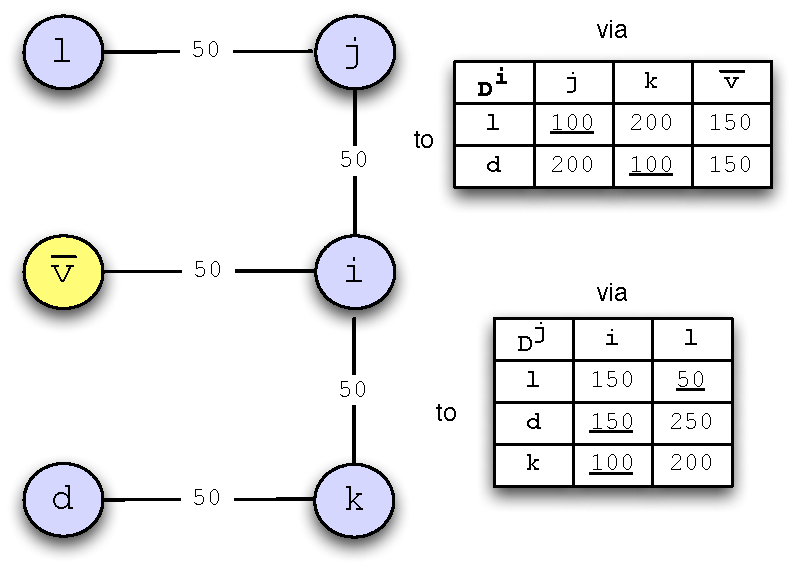
\includegraphics[scale=0.55]{figs/example-a-color.pdf}}
    \subfigure[After $\overline{v}$ is compromised. The dashed lines mark false paths claimed by $\overline{v}$.]
	{\label{fig:example-b}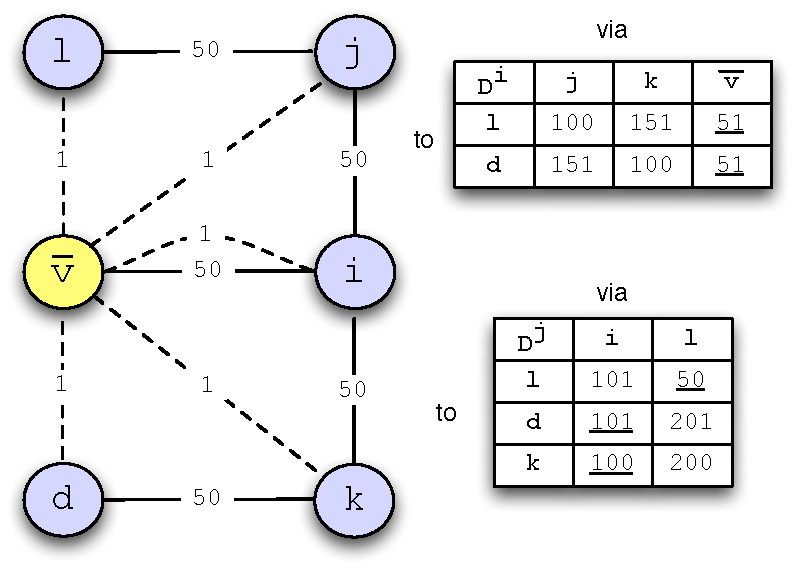
\includegraphics[scale=0.55]{figs/example-b-color.pdf}} 
    \subfigure[After recovery.]{\label{fig:example-c}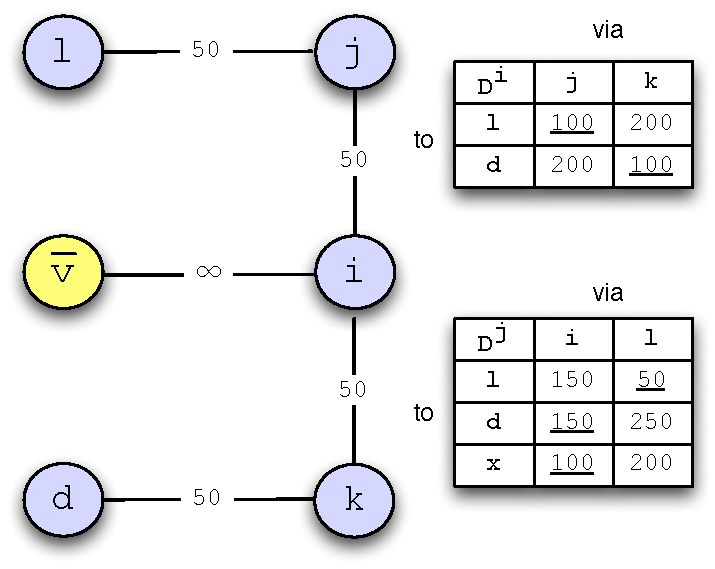
\includegraphics[scale=0.55]{figs/example-c-color.pdf}}
  \end{center}
	%\caption{Three snapshots of a graph, $G$.}
	\caption{Three snapshots of a graph, $G$, where $\overline{v}$ is the compromised node. Parts of $i$ and $j$'s distance matrix are displayed to the right of each sub-figure.
	The least cost values are underlined.}
	%$dmatrix_i$ and $dmatrix_j$ are displayed to the right of each sub-figure.
	%The least cost values are underlined.}
	%(a) $G$  before $\overline{v}$ is compromised, (b) $G$ after $\overrightarrow{bad}$ has}
	%has finished propagating but before recovery has started, and (c) $G$ after recovery. The dashed lines in (b) mark false paths used by $\overrightarrow{bad}$. 
	%Parts of $dmatrix_i$ and $dmatrix_j$ are displayed to the right of each sub-figure. The least cost values are underlined.}
  \label{fig:dv-example}
\end{figure*}


We trace the execution of \second using the example in Figure \ref{fig:dv-example}.
In Figure \ref{fig:example-b}, $i$ uses \bad to reach nodes $l$ and $d$.  $j$ uses $i$ to reach all nodes except $l$.  Notice that when $j$ uses $i$ to reach $d$, 
it transitively uses \badvector (e.g., uses path $j-i-$\bads$-d$ to $d$). 
After the preprocessing completes, $i$ selects a new neighbor to route through to reach $l$ and $d$ by finding its new smallest distance in \dmatrixi 
to these destinations: $i$ selects the routes via $j$ to $l$ with a cost of $100$ and $i$ picks the route via $k$ to reach $d$ with cost of $100$. 
(No changes are required to route to $j$ and $k$ because $i$ uses its direct link to these two nodes). 
Then, using traditional distance vector $i$ sends \minvi to $j$ and $k$.  When $j$ receives \minvis, $j$ must modify its distance to $d$ because \minvi indicates 
that $i$'s least cost to $d$ is now $100$.
$j$'s new distance value to $d$ becomes $150$, using the path $j-i-k-l$. $j$ then sends a message sharing \minvj with its neighbors.  From this point, recovery proceeds according 
by using traditional distance vector. 

%{\bf Pros/Cons.} 
\second is simple and makes no synchronization assumptions. % The primary advantage of \second is its simplicity.
However, \second is vulnerable to the \infinity problem. Because each node only has local information, the new shortest paths may continue to use \bads.
%When computing new shortest paths, a node cannot guarantee that the new shortest path does not use \bad because the node only has local information. 
For example, if $w(k,d)=400$ in Figure \ref{fig:dv-example}, a \infinity scenario would arise. After notification of \bads's compromise, 
$i$ would select the route via $j$ to reach $d$ with cost $151$ (by consulting \dmatrixis), using a path that does not actually exist in $G$ ($i-j-i-$\bads$-d$), since $j$ has removed \bad as a 
neighbor. When $i$ sends \minvi to $j$, $j$ selects the route via $i$
to $d$ with cost $201$. Again, the path $j-i-j-i-$\bads$-d$ does not exist.  In the next iteration, $i$ 
picks the route via $j$ having a cost of $251$. This process continues until each node finds their 
correct least cost to $d$.  We will see in our simulation study that the \infinity problem can incur significant message and time costs.




\subsection{The Purge Algorithm}
\label{subsec:purge}


\purge globally invalidates all false state using a diffusing computation and then uses distance vector to compute new distance values that avoid all invalidated paths.
Recall that diffusing computations preserve the decentralized nature of distance vector.
The diffusing computation is initiated at the neighbors of \bad because only these nodes are 
aware if \bad is used an intermediary node. The diffusing computations spread from \bads's neighbors to the network edge, invalidating false state at each node along the way. 
Then ACKs travel back from the network edge to the neighbors of \bads, indicating that the diffusing computation is complete. 
See Algorithm \ref{alg:purge} and \ref{alg:purge2} in the Appendix for a complete specification of this diffusing computation.

Next, \purge uses distance vector to recompute least cost paths invalidated by the diffusing computations.  In order to initiate the distance vector computation, each 
node is required to send a message after diffusing computations complete, even if no new least cost is found.  Without this step, distance vector may not correctly compute new least cost 
paths invalidated by the diffusing computations.  For example, consider the following the scenario when the diffusing computations complete: a node $i$ and all of $i$'s neighbors have 
least cost of $\infty$ to destination node $a$. Without forcing $i$ and its neighbors to send a message after the diffusing computations complete, neither $i$ nor $i$'s neighbors may
never update their least cost to $a$ because they may never receive a non-$\infty$ cost to $a$.

%{\footnote {\small The operations performed by the diffusing compuations described in Section \ref{subsec:preprocess} are  }
%This algorithm is specified in Algorithm \ref{alg:discover} of the Appendix.

In Figure \ref{fig:dv-example}, the diffusing computation executes as follows. First, $i$ sets its distance to $l$ and $d$ to $\infty$ (thereby invalidating $i$'s path to $l$ and $d$)
because $i$ uses \bad to route these nodes. Then, $i$ sends a message to $j$ and $k$ containing $l$ and $d$ as invalidated destinations.
When $j$ receives $i$'s message, $j$ checks if it routes via $i$ to reach $l$ or $d$. Because $j$ uses $i$ to reach $d$, $j$ sets its distance estimate to $d$ to $\infty$. 
$j$ does not modify its least cost to $l$ because $j$ does not route via $i$ to reach $l$. Next, $j$ sends a message that includes $d$ as an invalidated destination.
$l$ performs the same steps as $j$. After this point, the diffusing computation ACKs travel back towards $i$. When $i$ receives an ACK, the diffusing computation is complete. At this
point, $i$ needs to compute new least costs to node $l$ and $d$ because $i$'s distance estimates to these destinations are $\infty$. 
$i$ uses \dmatrixi to select its new route to $l$ (which is via $j$) and uses \dmatrixi to find $i$'s new route to $d$ (which is via $k$). Both new paths have cost $100$. Finally,
$i$ sends \minvi to its neighbors, triggering the execution of distance vector to recompute the remaining distance vectors.

Note that a consequence of the diffusing computation is that not only is all \badvector state deleted, but all \oldvector state as well.  
Consider the case when \bad is detected before node $i$ receives \badvectors.
It is possible that $i$ uses \oldvector to reach a destination, $d$. In this case, the diffusing computation will set $i$'s distance to $d$ to $\infty$.

An advantage of \purge is that it operates without the need for any clock synchronization.  We will find that \cprs, unlike \purges, either requires extra computation to maintain logical clocks or
assumes clocks are loosely synchronized. %no effort is required to synchronize clocks makes no synchronization assumptions. 
Also, \purges's diffusing computations ensure that the \infinity problem does not occur by removing
false state from the entire network. However, globally invalidating false state can be wasteful if valid alternate paths are locally available. 


\subsection{The CPR Algorithm}
\label{subsec:cpr}

\cprs {\footnote {\small The name is an abbreviation for {\bf C}heck{\bf P}oint and {\bf R}ollback. }} 
is our third and final recovery algorithm. 
Unlike \second and \purges, \cpr only requires that clocks across different
nodes be loosely synchronized i.e. the maximum clock offset between
any two nodes is assumed to be  bounded. For ease of explanation, we
describe \cpr as if the clocks at different nodes are perfectly
synchronized. Extensions to handle loosely synchronized clocks should
be clear. Accordingly, we assume that all neighbors of \bads, are
notified of the time, $t'$, at which \bad was compromised.  At the end of this section we comment on how the clock synchronization requirement assumption can be dropped by
using logical clocks.

For each node, $i \in G$, \cpr adds a time dimension to \minvi and \dmatrixis, which \cpr then uses to locally archive a complete history of values. 
Once the compromised node is discovered, 
the archive allows the system to rollback to 
a system snapshot from a time before \bad was compromised. From this point, \cpr needs to remove \bad and \oldvector and update stale distance values resulting from link weight changes.
We describe each algorithm step in detail. % (1) Create a \minv and \dmatrix archive. (2) roll back to a valid snapshot, and (3) steps after the rollback. 

{\bf Step 1: Create a \minv and \dmatrix archive.} 
	We define a  \emph{snapshot} of a data structure to be a copy of all current distance values along with a timestamp.
	{\footnote {\small In practice, we only archive distance values that have changed. Thus each distance value is associated with its own timestamp.}}
	The timestamp marks the time at which that set of distance values start being used. 
	\minv and \dmatrix are the only data structures that need to be archived. This approach is similar to ones used in temporal databases 
  \cite{Jensen91,Lomet06}.

  Our distributed archive algorithm is quite simple.  %For a given data structure, a node archives all current distance values whenever one of the values change. 
	Each node has a choice of archiving at a given frequency (e.g., every $m$ timesteps) or after some number of distance value changes (e.g., each time a distance 
	value changes).  Each node must choose the same option, which is specified as an input parameter to \cprs. A node archives independently of all other nodes.
  A side effect of independent archiving, is that even with perfectly synchronized clocks, the union of all snapshots may not constitute a globally consistent snapshot. 
  For example, a link weight change event may only have propagated 
  through part of the network, in which case the snapshot for some nodes will reflect this link weight change (i.e., among nodes that have learned of the event) 
  while for other nodes no local snapshot will reflect the occurrence of this event. We will see that a globally consistent snapshot is not required for correctness.  

{\bf Step 2: Rolling back to a valid snapshot.} 
Rollback is implemented using diffusing computations. Neighbors of the compromised node independently select a snapshot to roll back to, such that the snapshot is the most recent one taken
before $t'$.  Each such node, $i$, rolls back to this snapshot by restoring the \minvi and \dmatrixi values from the snapshot.  Then, $i$ initiates a diffusing computation to inform all other
nodes to do the same. If a node has already rolled back and receives an additional rollback message, it is ignored. 
(Note that this rollback algorithm ensures that no reinstated distance value uses \badvector because every node rolls back to a snapshot 
with a timestamp less that $t'$).  A pseudo-code specification of this rollback algorithm can be found in the Appendix (Algorithm \ref{alg:rollback}).  
%in the Appendix gives the pseudo-code for the rollback algorithm.


{\bf Step 3: Steps after rollback.} After Step 2 completes, the algorithm in Section \ref{subsec:preprocess} is executed.
There are two issues to address.
First, some nodes may be using \oldvectors.  Second, some nodes may have stale state as a result of link weight changes that occurred during $[t',t_b]$ and 
consequently are not reflected in the snapshot. 
To resolve these issues, each neighbor, $i$, of \bads, sets its distance to \bad to $\infty$ and then selects new least cost values that avoid the compromised node, triggering
the execution of distance vector to update the remaining distance vectors.  That is, for any destination, $d$, where $i$ routes via \bad to reach $d$,
$i$ uses \dmatrixi to find a new least cost to $d$. If a new least costs value is used, $i$ sends a distance vector message to its neighbors. Otherwise, $i$ sends no message.
Messages sent trigger the execution of distance vector.

During the execution of distance vector, each node uses the most recent link weights of its adjacent links. Thus, 
if the same link changes cost multiple times during  $[t',t_b]$, we ignore all changes but the most recent one. Algorithm \ref{alg:cpr} specifies Step 3 of \cprs.

In the example from Figure \ref{fig:dv-example}, the global state after rolling back is nearly the same as the snapshot depicted in Figure \ref{fig:example-c}:
the only difference between the actual system state and that depicted in Figure \ref{fig:example-c} is that in the former 
$(i,$\bads$)=50$ rather than $\infty$. Step 3 in \cpr makes this change.  Because no nodes use \oldvectors, no other changes take place.

Rather than using an iterative process to remove false state (like in \second and \purges), \cpr does so in one diffusing computation.
However, \cpr incurs storage overhead resulting from periodic snapshots of \minv and \dmatrixs.  Also, after rolling back, stale state may exist if link weight changes occur during $[t',t_b]$.
This can be expensive to update.
Finally, unlike \purge and \seconds, \cpr requires loosely synchronized clocks because without a bound on the clock offset, nodes may rollback to highly inconsistent local snapshots.
Although correct, this would severely degrade \cpr performance.

{\bf Using Logical Clock Timestamps.}
We can use Lamport's clock algorithm  \cite{Lamport78} to assign timestamps based on logical, rather than physical, clocks.  This allows us to drop the inconvenient assumption of loosely 
synchronized clocks. Here we briefly outline how the stated \cpr algorithm can be modified to use Lamport timestamps to create and restore system snapshots.

%First, \cpr is modified to create network-wide snapshots are periodically computed using diffusing computations instead of each node creating snapshots independently.   
First, \cpr is modified to create network-wide snapshots using diffusing computations instead of each node creating snapshots independently.   
Here each node records the logical timestamp when creating a checkpoint. 
The logical clock values are determined using the ``happened before'' relation defined by Lamport \cite{Lamport78}, where we limit events to be messages sent and received, and 
by piggybacking each node's logical clock value with each message it sends.  

%After being notified of \bads, each neighbor, $i$, of the compromised node determines the logical timestamp of the snapshot it wishes to restore.  
%This requires that either the detection algorithm specifies either \badvector or the logical time \bad was compromised. 
The second change to \cpr is in how each node determines the snapshot to restore during the roll back process (i.e., Step 2 above). Starting with each $i \in adj(\overline{v})$, 
$i$ determines the logical timestamp of the snapshot it wishes to restore.  This requires that the detection algorithm specifies either \badvector or the logical time \bad was compromised. 
In the latter case, finding the appropriate snapshot to restore is straightforward.
If only \badvector is provided, $i$ must additionally record each \minv vector received (as a part of standard distance vector messaging) 
along with the corresponding Lamport timestamp.  By doing so, this archive can be searched
to find the logical timestamp in which \badvector was first received at $i$.  Let $t_l$ denote this timestamp.  Next, $i$ initiates a diffusing computation instructing all other nodes 
to roll back to their most recent snapshot taken before $t_l$.  After this point, the diffusing computations continue as described in Step 2 above and Step 3 
remains unchanged.

Rolling back using logical timestamps does not guarantee that all \badvector state is removed because Lamport timestamps only provide partial ordering of events. 
With logical clocks, \cpr can be thought of as a best-effort approach to quickly removing false routing state by rolling back in time.  \cpr is still correct with logical clocks
for the reasons described in its correctness proof (Corollary \ref{cor:cpr-correct-single}).  
%This version of \cpr can be thought of as a best-effort approach to quickly removing false routing state.




\subsection{Multiple Compromised Nodes}
\label{subsec:mult}

Here we detail the necessary changes to each of our recovery algorithms when multiple nodes are compromised. Since we make the same changes to all three algorithms, we do not refer 
to a specific algorithm in this section. Let $\overline{V}$ refer to the set of nodes compromised at time $t'$. 

In the case where multiple nodes are simultaneously compromised, each recovery algorithm is modified such that for each $\overline{v} \in \overline{V}$, all $adj(\overline{v})$
are notified that \bad was compromised. 
%to accept a \emph{set} of compromised nodes, $\overline{V}$, as input (rather than a single node).  {\bf not really correct to refer to the set as input}
From this point, the changes to each algorithm are straightforward.  For example,
the diffusing computations described in Section  \ref{subsec:preprocess} are initiated at the neighbor nodes of each node in $\overline{V}$.
{\footnote {\small For \cprs, $t'$ is set to the time the first node is compromised.}}
%First, we augment the preceprocessing procedure described in Section \ref{subsec:preprocess}. In 
%the case where multiple nodes are simulataneously compromised, we modify the diffusing computations to remove all compromised nodes as a destination. %each of these nodes as a destination.

More changes are required to handle the case where an additional node is compromised during the execution of a recovery algorithm. Specifically, when another node is 
compromised, $\overline{v}_2$, we make the following change to the distance vector computation of each recovery algorithm.
{\footnote {\small {Recall that each of our recovery algorithms use distance vector to complete their computation.}} 
If a node, $i$, receives a distance vector message which includes a distance value to destination $\overline{v}_2$, then $i$ ignores said distance value and processes
the remaining distance values (if any exist) to all other destinations (e.g., where $d \neq \overline{v}_2$) normally.  If the message contains no distance information for any 
other destination $d \neq \overline{v}_2$, then $i$ ignores the message.
Because $\overline{v}_2$'s compromise 
triggers a diffusing computation to remove $\overline{v}_2$ as a destination, each node eventually learns the identity of $\overline{v}_2$, thereby allowing the node 
execute the specified changes to distance vector.

Without this change it is possible that the recovery algorithm will not terminate.  Consider the case of two compromised nodes, $\overline{v}_1$ and $\overline{v}_2$,
where $\overline{v}_2$ is compromised during the recovery triggered by $\overline{v}_1$'s compromise.  In this case, two executions of the recovery algorithm are triggered: one when
$\overline{v}_1$ is compromised and the other when $\overline{v}_2$ is compromised.
 Recall that all three recovery algorithms set all link weights to $\overline{v}_1$ to $\infty$ (e.g., $(v_i,\overline{v}_1)=\infty, \forall v_i \in adj(\overline{v}_1)$).
If the first distance vector execution triggered by $\overline{v}_1$'s compromise is not modified to terminate least cost computations to $\overline{v}_2$, the distance vector step of the 
recovery algorithm would never complete because the least cost to $\overline{v}_2$ is $\infty$. 







\section{Analysis of Algorithms}
\label{sec:analysis-summary}

Here we summarize the results from our analysis, the detailed proofs can be found in Appendix \ref{sec:analysis}.
Using a synchronous communication model, we derive communication complexity bounds for each algorithm.  Our analysis assumes: a graph with unit link weights of $1$,
that only a single node is compromised, and that the compromised node
falsely claims a cost of $1$ to every node in the graph. 
For graphs with fixed link weights, we find that the communication complexity of all three algorithms is bounded above by $O(mnd)$  where $d$ is the diameter, $n$ is the number of nodes, and $m$ the maximum out-degree of any node.

In the second part of our analysis, we consider graphs where link weights can change. Again, we assume a graph with unit link weights of $1$ and a single compromised node that declares a cost of $1$ to every node.
Additionally, we let link weights increase between the time the malicious node is compromised and the time at which error recovery is initiated.  
We assume that across all network links, the total increase in link weights is $w$ units.
We find that \cpr incurs additional overhead (not experienced by \second and \purges) because \cpr must update stale state after rolling back. 
\second and \purge avoid the issue of stale state because neither algorithm rolls back in time.  As a result, the message complexity for \second and \purge is still bounded by
$O(mnd)$ when link weights can change, while \cpr is not. \cprs's upper bound becomes $O(mnd) + O(wn^2)$. 





\section{Evaluation}
\label{sec:eval}

In this section, we use simulations to characterize the performance of each of our three recovery algorithms in terms of message and time overhead. 
Our goal is to illustrate the relative performance of our recovery algorithms over different topology types (e.g., \er graphs, Internet-like graphs) and
different network conditions (e.g., fixed link costs, changing link costs).


%We build a custom simulator with a synchronous communication model: nodes send and receive messages at fixed epochs.  In each epoch, a node receives a
%message from all its neighbors and performs its local computation.  In
%the next epoch, the node sends a message (if needed).   All algorithms
We build a custom simulator with a synchronous communication model as described in Section \ref{sec:analysis}. All algorithms
are deterministic under this communication model.
The synchronous communication model, although simple, yields
interesting insights into the performance of each of the recovery
algorithms. Evaluation of our algorithms using a more general
asynchronous communication model is currently under
investigation. However, we believe an asynchronous implementation
will demonstrate similar trends.  

%Except in the case where multiple nodes are compromised, we simulate the following scenario:
We simulate the following scenario: 
{\footnote {\small In Section \ref{subsubsec:many} we consider the case of multiple compromised nodes.  In that experiment we modify our simulation scenario
to consider a set of compromised nodes, $\overline{V}$, instead of \bads.}}
\begin{enumerate}
	\item Before $t'$, $\forall v \in V$ \minvv and \dmatrixv are correctly computed.

	\item At time $t'$, \bad is compromised and advertises a \badvector (a vector with a cost of $1$ to \emph{every} node in the network) to its neighboring nodes.

	\item \badvector spreads for a specified number of hops (this varies by experiment).  Variable $k$ refers to the number of hops that \badvector has spread.

	\item At time $t$, some node $v \in V$ notifies all $v \in adj($\bads$)$ that \bad was compromised. 
	{\footnote { \small For \cpr this node also indicates the time, $t'$, \bad was compromised.}} 

\end{enumerate}
The message and time overhead are measured in step (4) above. The pre-computation common to all three recovery algorithms, described in Section \ref{subsec:preprocess},
is not counted towards message and time overhead. We describe our simulation scenario for multiple compromised nodes in Section \ref{subsubsec:many}.


\subsection{Fixed Link Weight Experiments}
\label{subsec:fixed}

In the next five experiments, we evaluate our recovery algorithms over different topology types in the case of fixed link costs.

\subsubsection{Experiment 1 - \er Graphs with Fixed Unit Link Weights}
\label{subsubsec:expt1}

We start with a simplified setting and consider 
Erd\"{o}s-R\'enyi graphs with parameters $n$ and $p$. 
$n$ is the number of graph nodes and $p$ is the probability that link $(i,j)$ exists where $i,j \in V$.
The link weight of each edge in the graph is set to $50$.
We iterate over different values of $k$. For each $k$, we 
generate an Erd\"{o}s-R\'enyi graph, $G = (V,E)$, with parameters $n$ and $p$. Then we select a \bad $\in V$ uniformly at random and simulate the scenario described above, 
using \bad as the compromised node. In total we sample $20$ unique nodes for each $G$.
We set $n=100$, $p=\{0.05,0.15,0.25, 0.50\}$, and let $k=\{1,2,
... 10\}$. Each data point is an average over $600$ runs ($20$ runs over 
$30$ topologies).  We then plot the $90 \%$ confidence interval.

For each of our recovery algorithms, Figure \ref{fig:msg} shows the
message overhead for different values of $k$. %The $90 \%$ confidence interval is shown.
We conclude that \cpr outperforms \purge and \second across all topologies. \cpr performs well because \badvector is removed using a single diffusing computation,  
while the other algorithms remove \badvector state through distance vector's iterative process.
\cprs's global state after rolling back is almost the same as the final recovered state.

\begin{figure*}[t]
\centering
\subfigure[{$p=0.05$, diameter=$6.14$}]{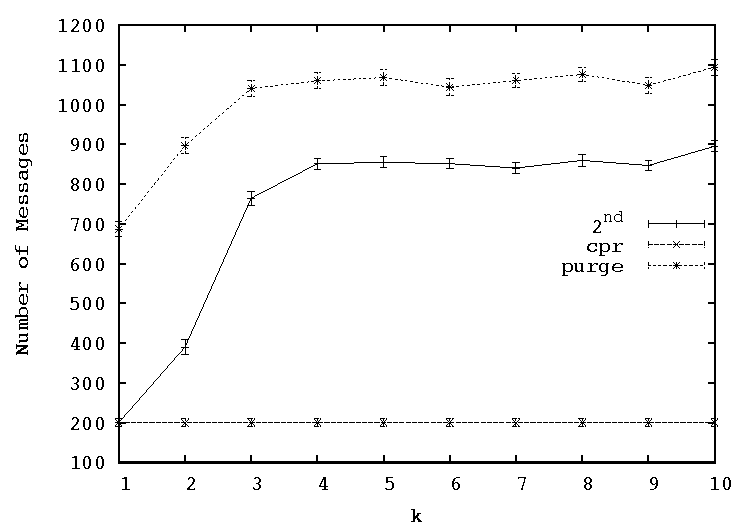
\includegraphics[width=0.32\textwidth]{figs/synch/msg5.pdf}}
\subfigure[{$p=0.15$, diameter=$3.01$}]{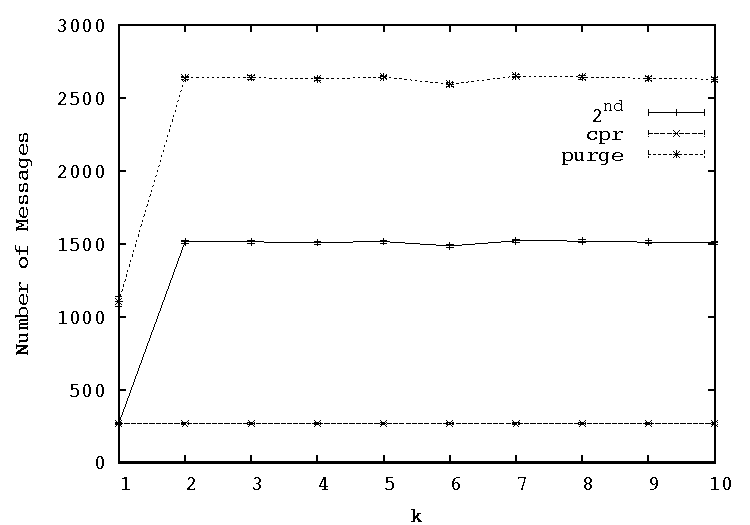
\includegraphics[width=0.32\textwidth]{figs/synch/msg15.pdf}}
\subfigure[{$p=0.25$, diameter=$2.99$}]{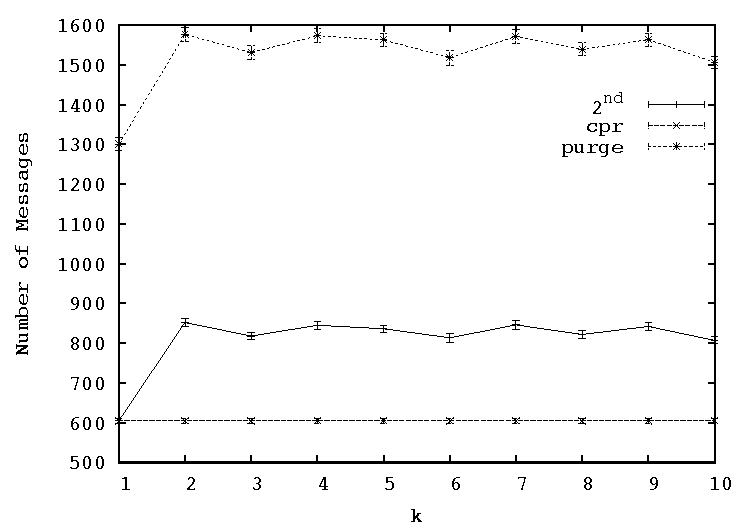
\includegraphics[width=0.32\textwidth]{figs/synch/msg25.pdf}}
\subfigure[{$p=0.50$, diameter=$2$}]{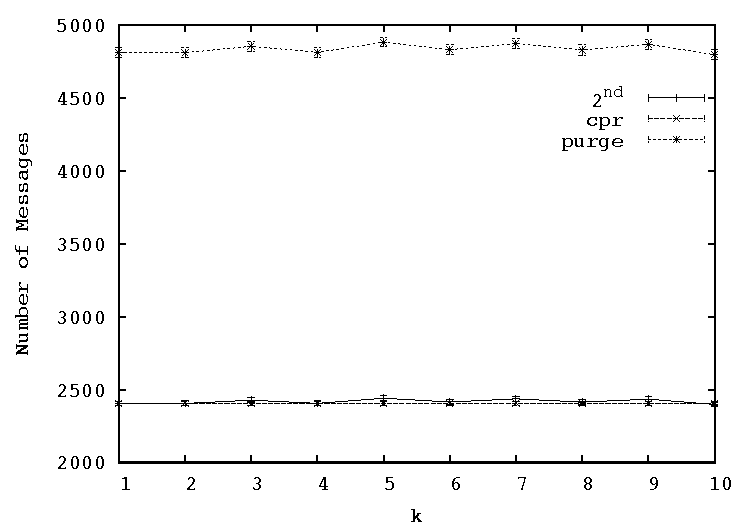
\includegraphics[width=0.32\textwidth]{figs/synch/msg50.pdf}}
%\subfigure[{Cumulative path cost decreases during the simulation}]{\includegraphics[width=0.49\textwidth]{figs/tsdecrease6.pdf}}
\caption{Experiment 1: message overhead for \er Graphs with Fixed Unit Link Weights generated over different $p$ values. Note the y-axis have different scales.}
\label{fig:msg}
\end{figure*}

\begin{figure*}[t]
\centering
\subfigure[{$p=0.05$, diameter=$6.14$}]{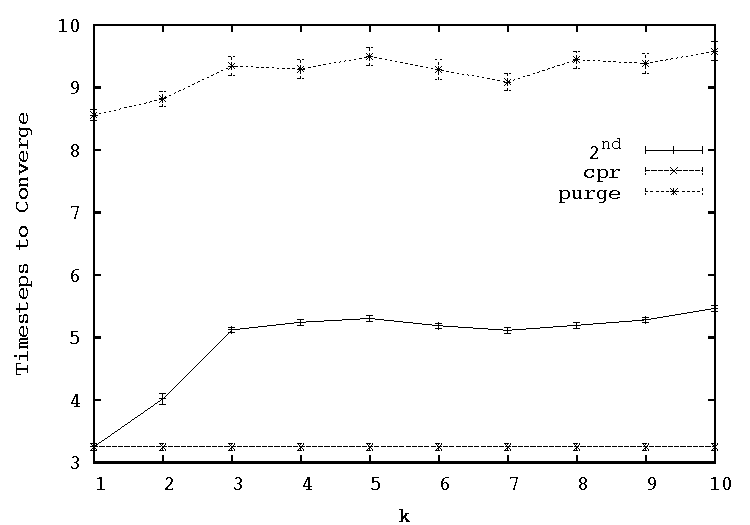
\includegraphics[width=0.32\textwidth]{figs/synch/epoch5.pdf}}
\subfigure[{$p=0.15$}, diameter=$3.01$]{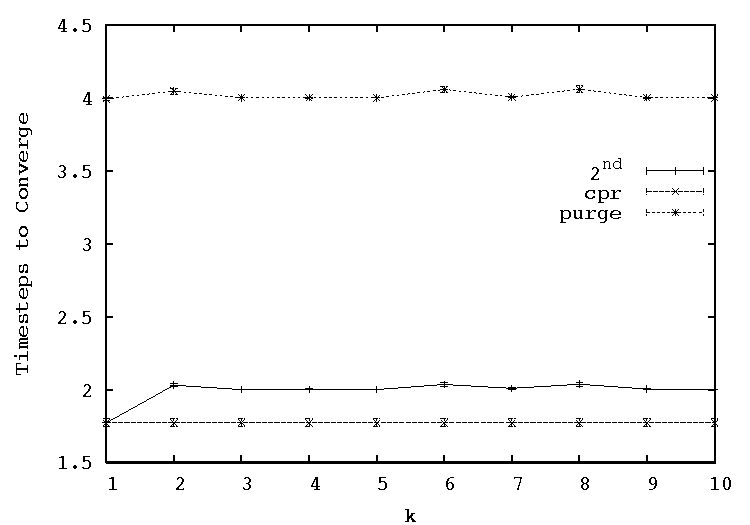
\includegraphics[width=0.32\textwidth]{figs/synch/epoch15.pdf}}
\subfigure[{$p=0.25$}, diameter=$2.99$]{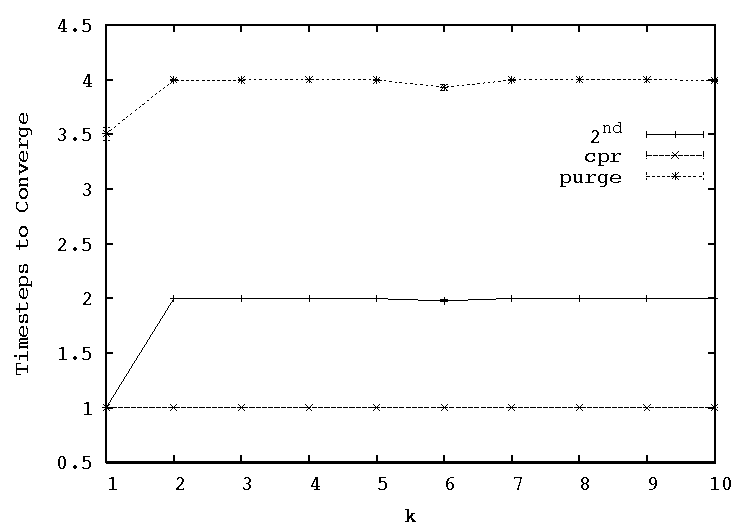
\includegraphics[width=0.32\textwidth]{figs/synch/epoch25.pdf}}
\subfigure[{$p=0.50$}, diameter=$2$]{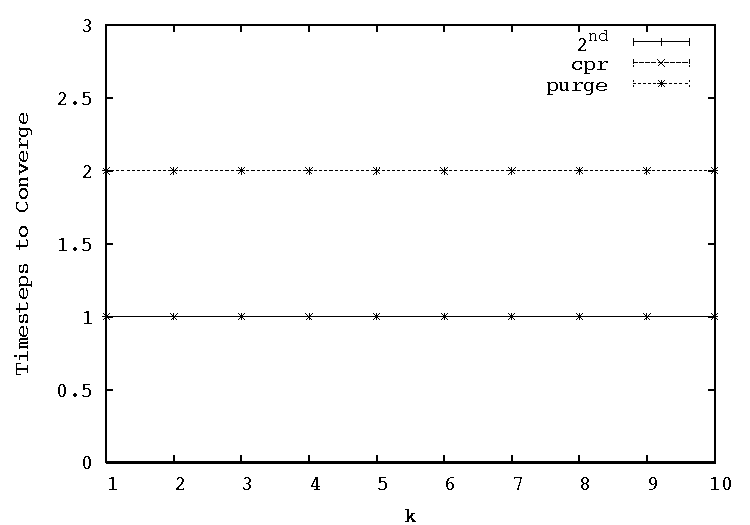
\includegraphics[width=0.32\textwidth]{figs/synch/epoch50.pdf}}
%\subfigure[{Cumulative path cost decreases during the simulation}]{\includegraphics[width=0.49\textwidth]{figs/tsdecrease6.pdf}}
\caption{Experiment 1: time overhead for \er Graphs with Fixed Unit Link Weights generated over different $p$ values.}
\label{fig:epoch}
\end{figure*} 


%In other words, \cpr performs well because its global state  (recall we define the global state of the routers as the union of their local states) is almost the same as the final recovered state.
%Specifically, if we let $S'$ represent the global state after rolling back and let $S$ be the final recovered state, the only difference between $S$ and $S'$, is that $S'$ 
%contains state that depends directly or transitively on \oldvector while $S$ does not. 
%\cpr performs exactly the same as \second at $k=1$ because \second at $k=1$ also must only remove \oldvector state and uses the same iterative process as \cprs. 
%For this reason, across all $k$ values, \cpr performs exactly the same as \second at $k=1$.  {\bf note:} {\it may need to elaborate more here.}

\second recovery can be understood as follows.  By Corollary \ref{cor:startbad} and \ref{cor:during} in Section \ref{subsec:trends}, distance values increase from their initial value until they 
reach their final (correct) value. Any intermediate, non-final, distance value uses \badvector or \oldvectors. Because \badvector and \oldvector no longer exist during recovery,
these intermediate values must correspond to routing loops.
%In this experiment, with \second distance estimates quickly count up to their final value.
Table \ref{tab:loop1} shows that there are few pairwise routing loops during \second recovery in the network scenarios generated in Experiment 1, 
indicating that \second distance values quickly count up to their final value.
{\footnote {\small We compute this metric as follows. After each simulation timestep, we count all pairwise routing loops over all source-destination pairs and then sum all of these values.}}
Although no pairwise routing loops exist during \purge recovery, \purge incurs overhead in performing network-wide state invalidation. Roughly, $50\%$ of \purges's messages come from these
diffusing computations. 
For these reasons, \purge has higher message overhead than \seconds.

Figure \ref{fig:epoch} shows the time overhead for the same $p$ values. The trends for time overhead match the trends we observe for message overhead. 
{\footnote {\small For the remaining experiments, we omit time overhead plots because time overhead follows the same trends as message overhead.}}


\begin{table}
\begin{center}
\begin{tabular}{l|l|l|l|l}
 & $k=1$&  $k=2$ & $k=3$ & $k=4-10$ \\
\hline
 $p=0.05$  & $0$ & $14$ & $87$ &  $92$ \\
 $p=0.15$  & $0$ & $7$&  $8$ & $9$ \\
 $p=0.25$  & $0$ & $0$ & $0$ &  $0$ \\
 $p=0.50$  & $0$ & $0$ & $0$ &  $0$ \\
 %$p=\{0.15,0.25,0.50\}$  & $0$ & $0$&  $0$ & $0$ \\
\end{tabular}
\end{center}
\caption{Average number pairwise routing loops for \second in Experiment 1.}
%$p=.50$ for Experiment 1 is omitted because no pairwise routing loops are found across all $k$ values.} 
\label{tab:loop1}
\end{table}

\begin{table}
\begin{center}
\begin{tabular}{l|l|l|l|l}
 & $k=1$&  $k=2$ & $k=3$ & $k=4-10$ \\
\hline
  $p=0.05$  & $554$ & $1303$ & $9239$ &  $12641$ \\
 $p=0.15$  & $319$ & $698$&  $5514$ & $7935$ \\
 $p=0.25$  & $280$ & $446$ & $3510$ &  $5440$ \\
 $p=0.50$  & $114$ & $234$ & $2063$ &  $2892$ \\
 %$p=\{0.15,0.25,0.50\}$  & $0$ & $0$&  $0$ & $0$ \\
\end{tabular}
\end{center}
\caption{Average number pairwise routing loops for \second in Experiment 2.}
%$p=.50$ for Experiment 1 is omitted because no pairwise routing loops are found across all $k$ values.} 
\label{tab:loop2}
\end{table}


\purge and \second message overhead increases with larger $k$. Larger $k$ imply that false state has propagated further in the network, 
implying more paths to repair, and therefore increased messaging.
For values of $k$ greater than a graph's diameter, the message overhead remains constant, as expected. 

%However, once $k$ is equal the graph diameter, $d$, the message overhead and number of epochs do not change for larger values of $k$ for a given topology. By definition, the graph diameter is
%the longest shortest path and so it follows that when $k > d$, each $v \in V'$ has a path less than $k$ hops to all destinations.  Therefore each $v$, does not use the $k$ hop path to \bads.
%For this reason, the message overhead (and number of epochs) do not change for $k>d$. {\bf todo verify if this is correct}

%Figure \ref{fig:compare} shows that for most values of $k$, if we do not count the epochs that occurred during \purges's purge phase 
%(e.g., only count \purges's discovery phase epochs), the resulting epoch omplexity is lower than \seconds's epoch complexity. When $k>2$, \second has higher epoch complexity 
%because the \infinity problem occurs with \second and not with \purges.  Table \ref{tab:loop1} shows that when $k>2$ there are pairwise routing loops during \second recovery, while

%The exception to this trend is when $k=1$ for all topologies and $k=2$ for $p=.05$: \purges's discovery phase epoch complexity is higher than \seconds's total epoch complexity. 
%In these cases, there are no or few pairwise routing loops for \seconds.  In this way, this is an ideal case for \second recovery. 
%Meanwhile, there are several cases in which distance values that previously used \oldvectors, which do not require messaging for \second but do for \purges.  
%Recall that \purge sets all distances that use \badvector or \oldvector to $\infty$ in its purge phase, so for \purge all distances using \oldvector must be recomputed. 
%With \seconds, many of these same distance values do not require re-computation: the actual path changes such as not to use \oldvector but the distance does not change because an 
%alternate path of the same distance is locally selected (since the distance does not change, no message is sent).


\subsubsection{Experiment 2 - \er Graphs with Fixed but Randomly Chosen Link Weights}
\label{subsec:expt2}


The experimental setup is identical to Experiment 1 with one exception: link weights are selected uniformly at random between $[1,n]$ (rather than using 
fixed link weight of $50$).

Figure \ref{fig:msg-rand} show the message overhead for different $k$ where $p=\{0.05,0.15,0.25,0.50 \}$. 
%We omit the figures for the other $p$ values because they follow the same trend as $p=.05$.
In striking contrast to Experiment 1, \purge outperforms \second for most values of $k$. 
\second performs poorly because the \infinity problem: Table \ref{tab:loop2} shows the large average number of pairwise routing loops in this experiment, 
an indicator of the occurrence of \infinity problem.
In the few cases (e.g., $k=1$ for $p=0.15$, $p=0.25$ and $p=0.50$) that \second performs better than \purges, \second has few routing loops.

No routing loops are found with \purges. \cpr performs well for the same reasons described in Section \ref{subsubsec:expt1}.  

\begin{figure*}[t]
\centering
\subfigure[{$p=0.05$, diameter=$6.14$}]{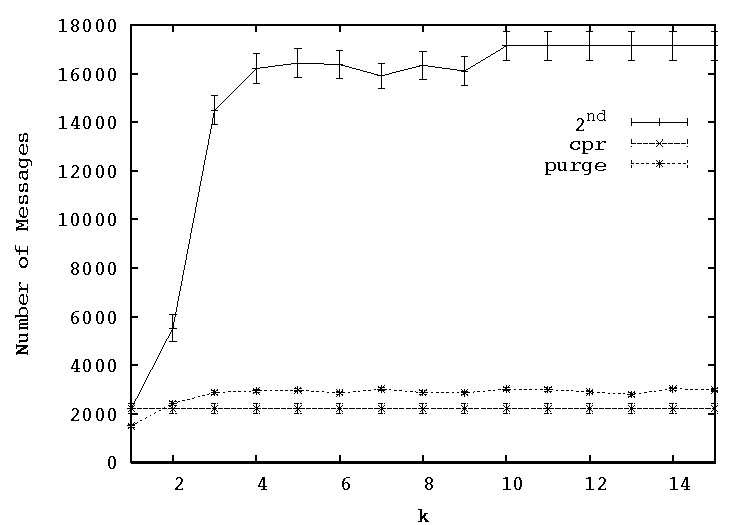
\includegraphics[width=0.32\textwidth]{figs/synch/msg-rand5.pdf}}
\subfigure[{$p=0.15$, diameter=$3.01$}]{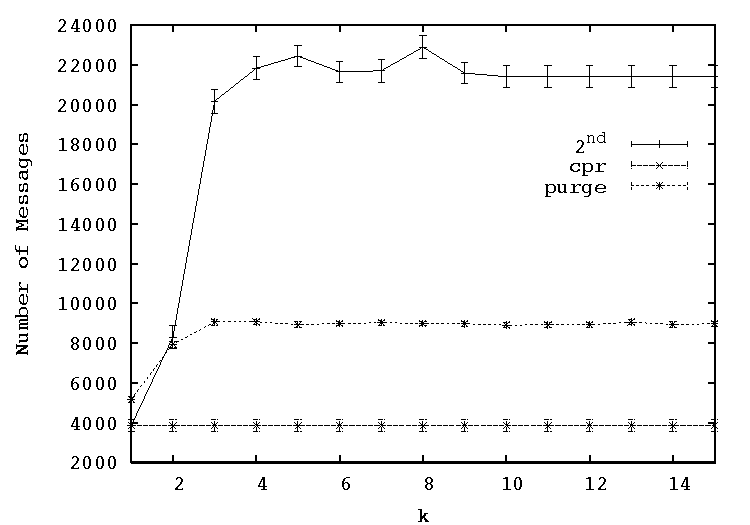
\includegraphics[width=0.32\textwidth]{figs/synch/msg-rand15.pdf}}
\subfigure[{$p=0.25$, diameter=$2.99$}]{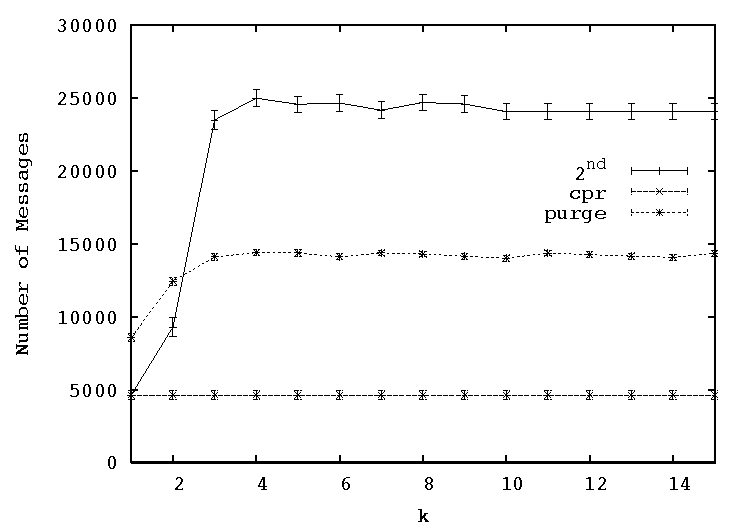
\includegraphics[width=0.32\textwidth]{figs/synch/msg-rand25.pdf}}
\subfigure[{$p=0.50$, diameter=$2$}]{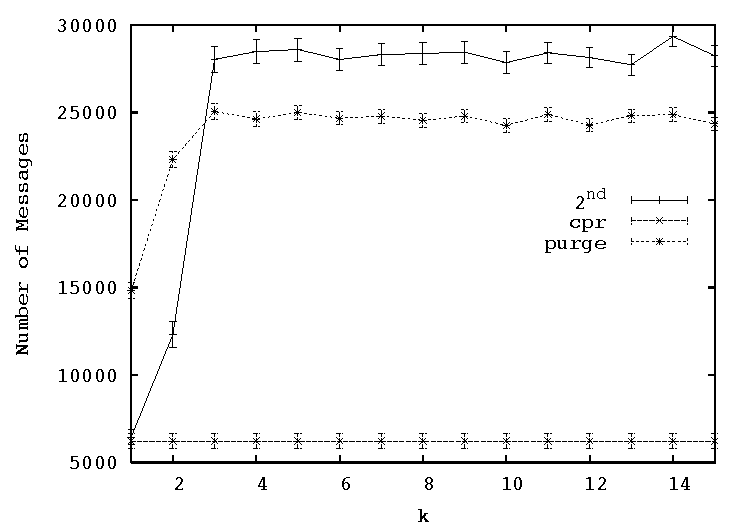
\includegraphics[width=0.32\textwidth]{figs/synch/msg-rand50.pdf}}
\caption{Experiment 2: message overhead for \er graph with link weights selected uniformly random from $[1,100]$. Note the y-axis have different scales.}
\label{fig:msg-rand}
\end{figure*}

%\begin{figure*}[t]
%\centering
%\subfigure[{$p=0.05$, diameter=$6.14$}]{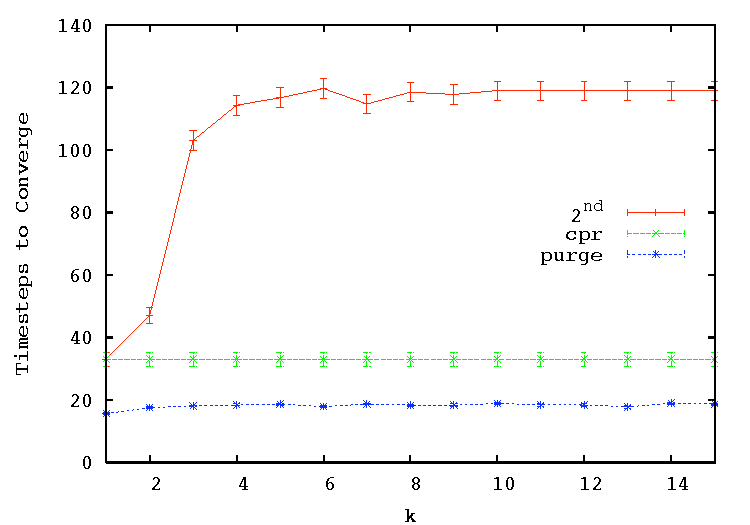
\includegraphics[width=0.32\textwidth]{figs/synch/epoch-rand5.pdf}}
%\subfigure[{$p=0.15$, diameter=$3.01$}]{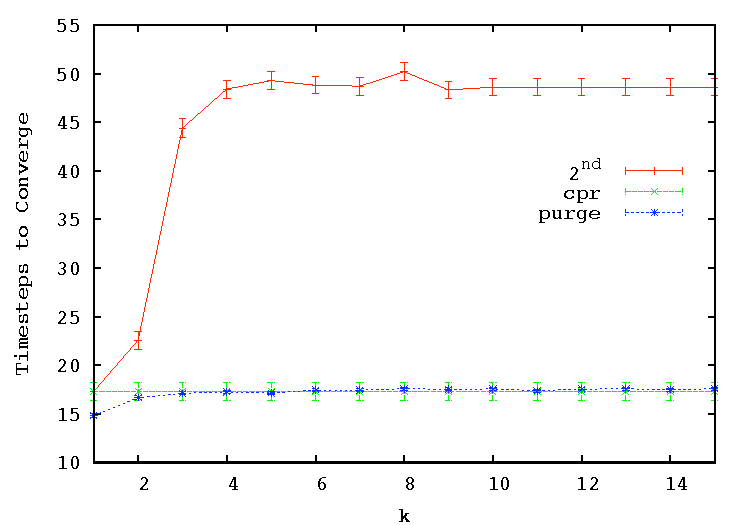
\includegraphics[width=0.32\textwidth]{figs/synch/epoch-rand15.pdf}}
%\subfigure[{$p=0.25$, diameter=$2.99$}]{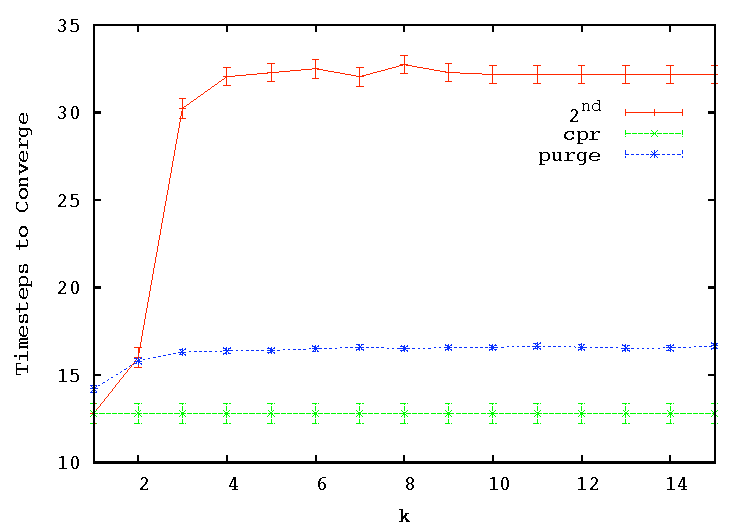
\includegraphics[width=0.32\textwidth]{figs/synch/epoch-rand25.pdf}}
%\subfigure[{$p=0.50$, diameter=$2$}]{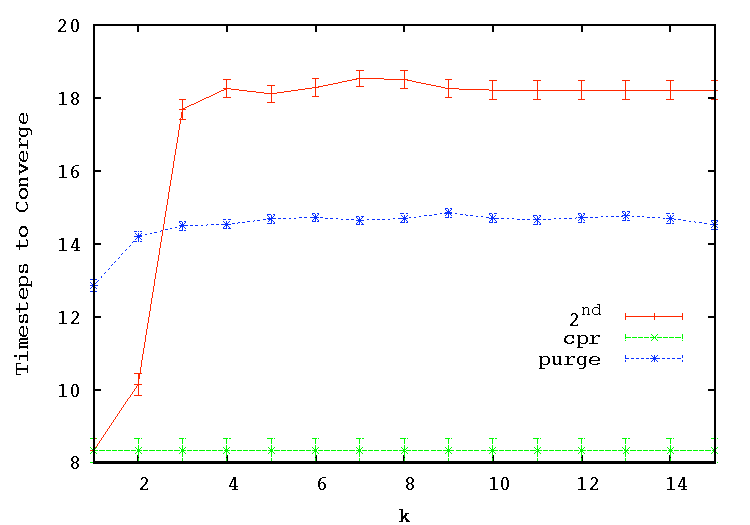
\includegraphics[width=0.32\textwidth]{figs/synch/epoch-rand50.pdf}}
%\subfigure[{Cumulative path cost decreases during the simulation}]{\includegraphics[width=0.49\textwidth]{figs/tsdecrease6.pdf}}
%\caption{Time overhead for \er graph with link weights selected uniformly random from $[1,100]$}
%\label{fig:epoch-rand}
%\end{figure*} 

%Recall that in Experiment 1, no pairwise routing loops are found when $p=0.15,p=0.25,$ and $p=0.50$.  The only pairwise routing loops in Experiment 1 
%are found when $p=0.05$, where a maximum of only $100$ pairwise routing loops occur. For \purges, no pairwise routing loops were found. {\bf Self-note}: {\it verify}.

In addition, we counted the number of epochs in which at least one pairwise routing loop existed.  For \second (across all topologies), on average, all but the last three 
timesteps had at least one routing loop.  This suggests that the \infinity problem dominates the cost for \seconds. 
%In some cases (e.g., $k=1$ for $p=.15$ and $p=.50$) \second performs better than \purges.  In these cases, \second has few routing loops.
%Table \ref{tab:loop} shows that there are fewer routing loops for small $k$. This is the case because with small $k$ there are fewer nodes using \badvectors. 

%The performance gap between \second and \purge shrinks with larger $p$ because with \second there are fewer routing loops with larger $p$.  
%This is consistent with our intuition:  larger $p$ values imply there are more alternate paths that do not use \badvectors.
%and thus routing loops are quickly exited because a low cost alternate path is used. 





\subsubsection{Experiment 3 - Internet-like Topologies}

%\begin{figure*}[t]
%\centering
%\subfigure[{AT\&T}]{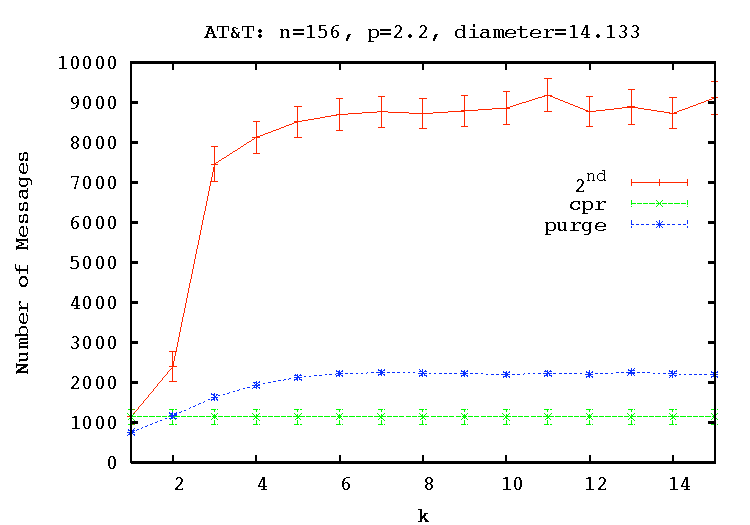
\includegraphics[width=0.32\textwidth]{figs/synch/att-msg.pdf}}
%\subfigure[{Rocketfuel 6461}]{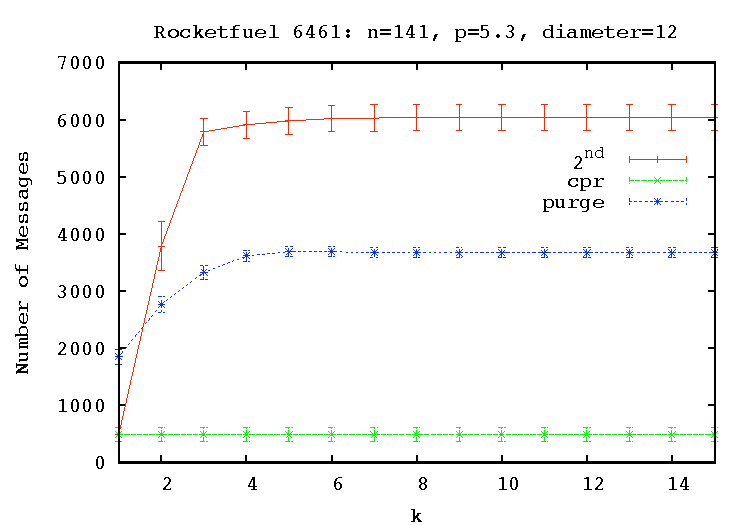
\includegraphics[width=0.32\textwidth]{figs/synch/rocket-msg6461.pdf}}
%\subfigure[{Rocketfuel 3867}]{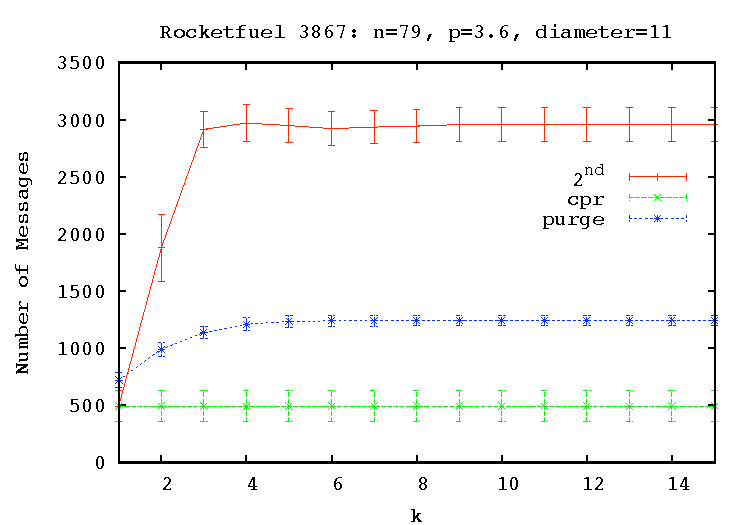
\includegraphics[width=0.32\textwidth]{figs/synch/rocket-msg3867.pdf}}
%\subfigure[{Cumulative path cost decreases during the simulation}]{\includegraphics[width=0.49\textwidth]{figs/tsdecrease6.pdf}}
%\caption{Real graph message overhead}
%\label{fig:msg-real}
%\end{figure*}


\begin{figure*}[t]
\centering
\subfigure[{GT-ITM, $n=156$, diameter=$14.133$}]{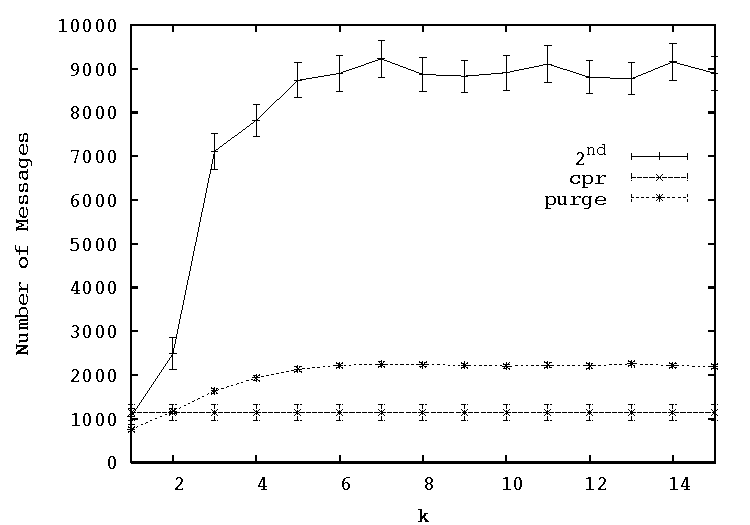
\includegraphics[width=0.32\textwidth]{figs/synch/msg-att.pdf}}
\subfigure[{Rocketfuel 6461, $n=141$, diameter=$8$}]{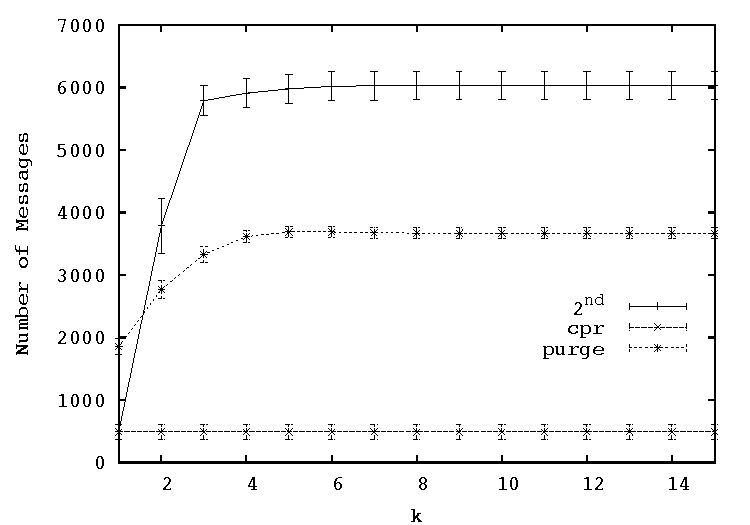
\includegraphics[width=0.32\textwidth]{figs/synch/msg6461.pdf}}
\subfigure[{Rocketfuel 3867, $n=79$, diameter=$10$}]{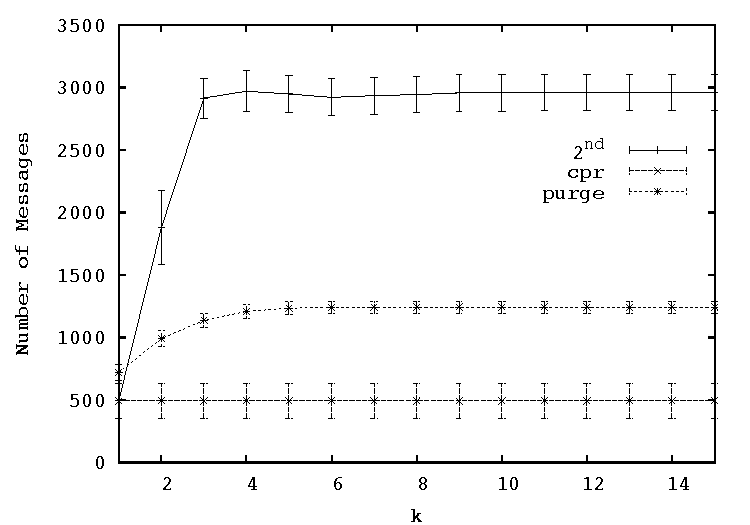
\includegraphics[width=0.32\textwidth]{figs/synch/msg3867.pdf}}
\caption{Experiment 3: Internet-like graph message overhead}
\label{fig:msg-real}
\end{figure*}

%\begin{figure*}[t]
%\centering
%\subfigure[{GT-ITM, $n=156$, average node degree=$2.2$, diameter=$14.133$}]{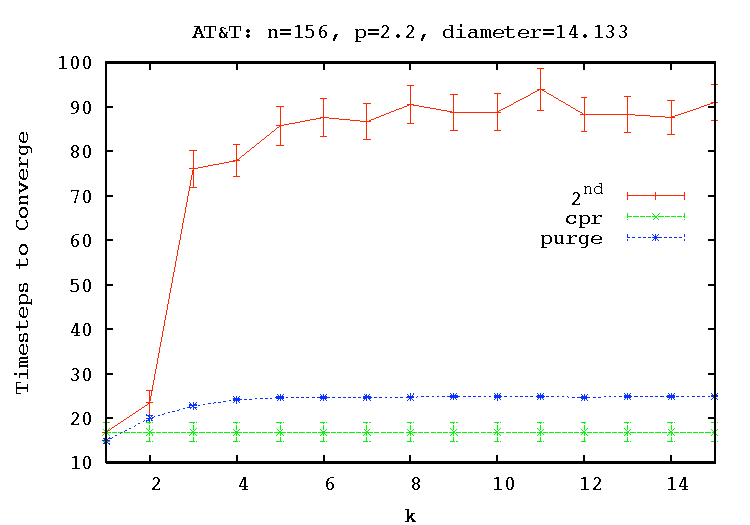
\includegraphics[width=0.32\textwidth]{figs/synch/att-epoch.pdf}}
%\subfigure[{Rocketfuel 6461, $n=141$, average node degree=$2.62$, diameter=$12$}]{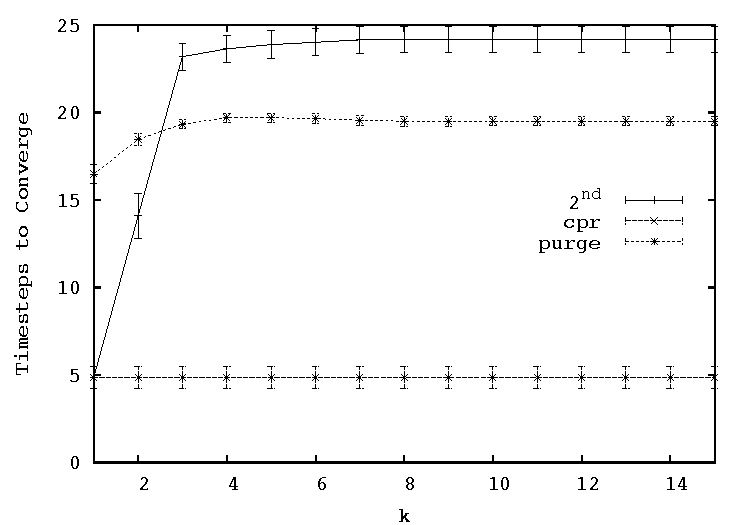
\includegraphics[width=0.32\textwidth]{figs/synch/rocket-epoch6461.pdf}}
%\subfigure[{Rocketfuel 3867, $n=79$, average node degree=$1.8$, diameter=$10$}]{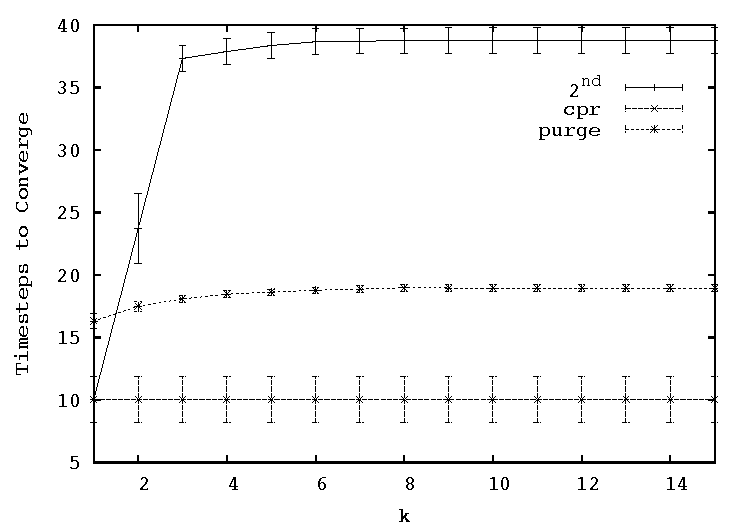
\includegraphics[width=0.32\textwidth]{figs/synch/rocket-epoch3867.pdf}}
%\subfigure[{Cumulative path cost decreases during the simulation}]{\includegraphics[width=0.49\textwidth]{figs/tsdecrease6.pdf}}
%\caption{Number of epochs/timesteps for real graphs}
%\label{fig:epoch-real}
%\end{figure*} 



Thus far, we studied the performance of our recovery algorithms over \er graphs, which have provided us with useful intuition about the performance
of each algorithm. In this experiment, we simulate our algorithms over Internet-like topologies downloaded from the Rocketfuel website \cite{Rocketfuel} and generated using GT-ITM 
\cite{GT-ITM}.  The Rocketfuel topologies have inferred edge weights. For each Rocketfuel topology, we let each node be
the compromised node and average over all of these cases for each value of $k$.  For GT-ITM, we used the parameters specified in Heckmann et al \cite{Heckmann} for  the $154$-node AT\&T topology
described in Section 4 of \cite{Heckmann}. For the GT-ITM topologies, we use the same criteria specified in Experiment 1 to generate each data point. 

The results, shown in Figure \ref{fig:msg-real}, follow the same pattern as in Experiment 2.  
%Due to space limitations, we only show the results for one representative topology.  The results for the other topologies follow the same pattern \cite{Tech}. 
In the cases where \second performs poorly,
the \infinity problem dominates the cost, as evidenced by the number of pairwise routing loops. In the few cases that \second performs better than \purges, there 
are few pairwise routing loops.

\subsubsection{Experiment 4 - Multiple Compromised Nodes}
\label{subsubsec:many}

In this experiment, we evaluate our recovery algorithms when multiple nodes are compromised. Our experimental setup is different from what we have used to this point:
we fix $k=\infty$ and vary the number of compromised nodes. Specifically, for each topology we create $m = \{1,2, ... , 15\}$ compromised nodes, each of which is selected  
uniformly at random (without replacement).  We then simulate the scenario described at the start of Section \ref{sec:eval} with one modification: $m$ nodes are 
compromised during $[t',t'+ 10]$. %We set $\Delta$ such that the recovery algorithm does not need to be restarted (as described in Section \ref{subsec:mult}).
The simulation is setup so that the outside algorithm identifies all $m$ compromised node at time $t$. %This eliminates the need to terminate and restart any recovery algorithm.
After running the simulation for all possible values for $m$, we generate a new topology and repeat the above procedure. 
We continue sampling topologies until the $90\%$ confidence interval for message overhead falls within $10\%$ of the mean message overhead. 

First, we perform this experiment using \er graphs with fixed link costs.  The message overhead results are shown in Figure \ref{fig:many-fixed}(a) for $p=0.05$ and $n=100$. 
{\footnote {\small We do not include the results for $p=\{0.15,0.25,0.50\}$ because they are consistent with the results for $p=0.05$.}}
The relative performance of the three algorithms is consistent with the results from Experiment 1, in which we had a single compromised node.
%We find the same trends we observed in Experiment 1 for large $k$ values in which there was a single compromised node.
As in Experiment 1, \second and \cpr have few pairwise routing loops (Figure \ref{fig:many-fixed}(b)).  In fact, there is more than an order of magnitude fewer pairwise routing 
loops in this experiment
when compared to the results for the same simulation scenario of $m$ compromised nodes using \er graphs with random link weights (Figure \ref{fig:many}(b)).
%The small number of pairwise routing loops is particularily evident when contrasted with the large number of pairwise routing loops 
%found with \er graphs with random link weights (Figure \ref{fig:many}(b)).  
Few routing loops imply that \second and \cpr (after rolling back) quickly count up to correct least costs.
In contrast, \purge has high message overhead because \purge globally invalidates false state before computing new least cost paths, rather than directly using alternate paths that 
are immediately available when recovery begins at time $t$. 
%The diffusing compuations are unnecessary in this scenario because many new least cost paths can be computed using local state information (demonstrated by \seconds's performance).

\second and \purge message overhead are nearly constant for $m \geq 8$ because at that point \badvector state has saturated $G$.
Figure \ref{fig:many-fixed} shows the number of least cost paths, per node,
that use \badvector or \oldvector at time $t$ (e.g., after \badvector state has propagated $k$ hops from \bads).  The number of least cost paths that use \badvector is nearly constant for $m \geq 8$. 

In contrast, \cpr message overhead increases with the number of compromised nodes.  After rolling back, \cpr must remove all compromised nodes and all
stale state (e.g., \oldvectors) associated with each \bads. As seen in Figure \ref{fig:many-fixed}(c), 
the amount of \oldvector state increases as the number of compromised nodes increase. 

Next, we perform the same experiment using \er graphs with with link weights selected uniformly at random from $[1,100]$. We only show the results for $p=.05$ and $n=100$ because the 
trends are consistent for other values of $p$.
The message overhead results for this experiment are shown in Figure \ref{fig:many}(a). \purge performs best because, unlike \second and \cprs, \purge does not suffer 
from the \infinity problem.  Below, we explain the performance of each algorithm in detail.

Consistent with Experiment 2 and 3, \second performs poorly because of the \infinity problem. 
Figure \ref{fig:many}(b) shows that a significant number of pairwise routing loops occur during \second recovery.  
\second message overhead remains constant when $m \geq 6$ because at this point \badvector state has saturated the network.  
Figure \ref{fig:many}(c) confirms this: the number of effected least cost paths remains constant (at $80$) for 
all $m \geq 6$. 

%\cpr also has a significant number of pairwise routing because after rolling back \cpr uses
%standard distance vector to compute new least cost paths for all paths using stale \oldvector state. Figure \ref{fig:many}(b) shows that the amount of \oldvector state increases as the
%number of compromised nodes increase, resulting in more routing loops for \cprs.

\cpr message overhead increases with the number of compromised nodes because the amount of \oldvector state increases as the number of compromised nodes increase (Figure \ref{fig:many}(c)). 
More \oldvector state results in more routing loops -- as shown in Figure \ref{fig:many}(b) -- causing increased message overhead.

%As with previous experiments,
\purge performs well because unlike \cpr and \seconds, no routing loops occur during recovery. %Figure \ref{fig:many}(b) shows that many pairwise routing loops occur during \second and \cpr recovery. 
Surprisingly, \purges's message overhead decreases when $m \geq 5$.  Although more 
least cost paths need to be computed with larger $m$, the message overhead decreases because the residual graph, $G'$, -- resulting from the removal of all $m$ compromised nodes -- is 
smaller than $G$.  As a result, there are $m$ fewer destinations and $m$ fewer nodes sending messages during the recovery process.
%As seen in Figure \ref{fig:many}(b), pairwise routing loops are prominent with both \second and \cprs. 

%used same topology for Rocketfuel ...
Finally, we simulated the same scenario of $m$ compromised node using the Internet-like graphs from Experiment 3. 
%{\footnote {\small For each Rocketfuel topology, we repeatidly selected $m$ compromised nodes until }}
The results were consistent with those for \er graphs with random link weights. % and therefore we do not present results for Internet-like graphs with multiple compromised nodes.



%Figure \ref{fig:many}(b) shows that the number of pairwise routing loops increases as the number of compromised nodes increases.  When $m \geq 6$, 
%in additional message overhead because more routing loops are processed per message. 
%{\bf think i want to remove the section about infinity message plot and the explanation about the number of loops per message}

\begin{figure*}[t]
\centering
\subfigure[{Message Overhead}]{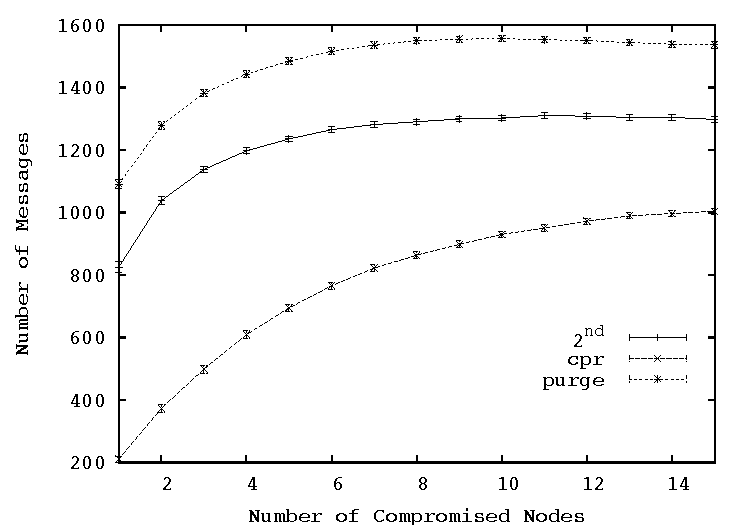
\includegraphics[width=0.32\textwidth]{figs/synch/many-fixed.pdf}}
\subfigure[{Pairwise Routing Loops}]{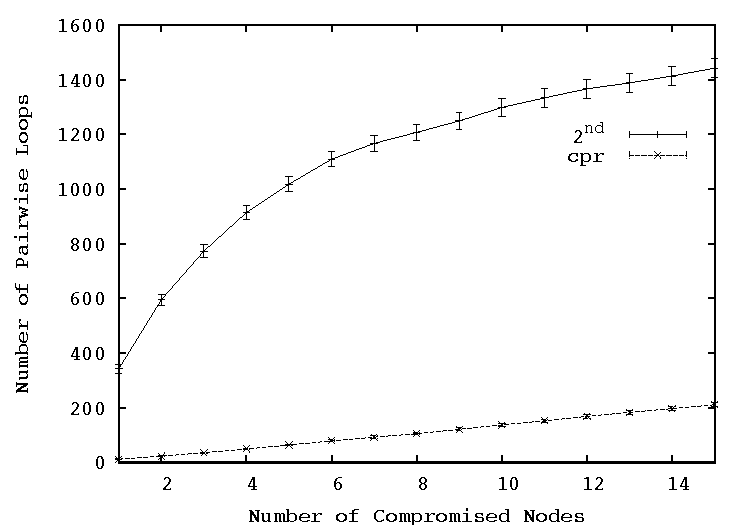
\includegraphics[width=0.32\textwidth]{figs/synch/loops-fixed.pdf}}
\subfigure[{Number of Effected Least Cost Paths}]{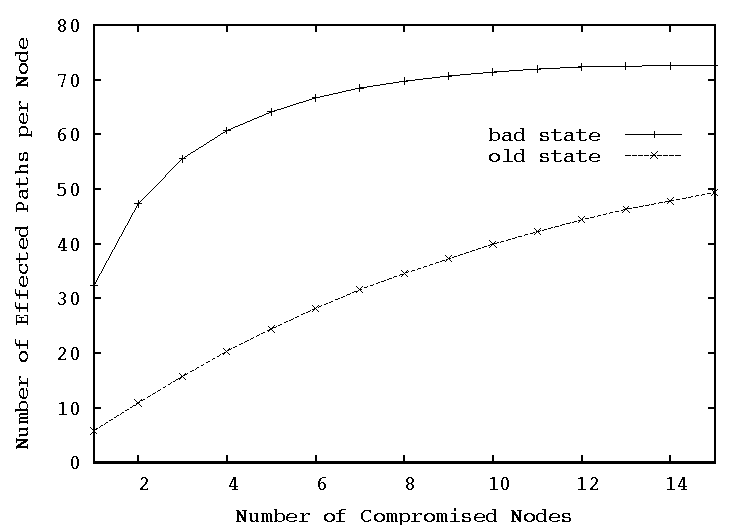
\includegraphics[width=0.32\textwidth]{figs/synch/initial-fixed.pdf}}
\caption{Experiment 4 - multiple compromised nodes over \er graphs with fixed link weights, $p=.05$, $n=100$, and diameter=$6.14$.}
\label{fig:many-fixed}
\end{figure*}



\begin{figure*}[t]
\centering
\subfigure[{Message Overhead}]{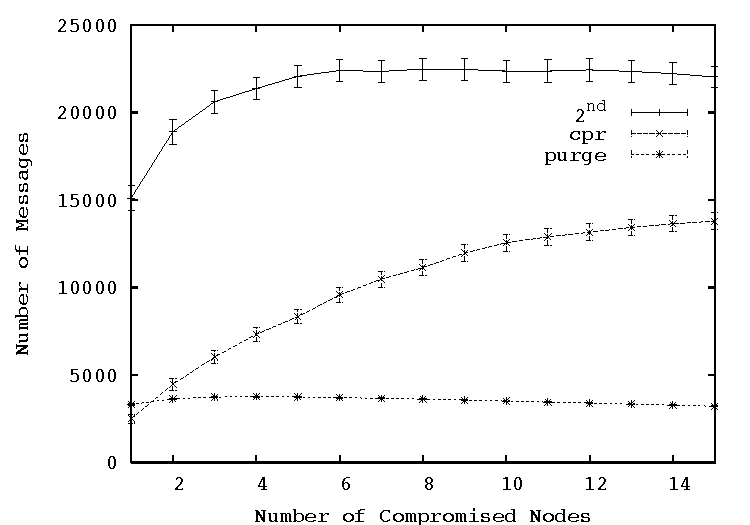
\includegraphics[width=0.32\textwidth]{figs/synch/many-rand.pdf}}
\subfigure[{Pairwise Routing Loops}]{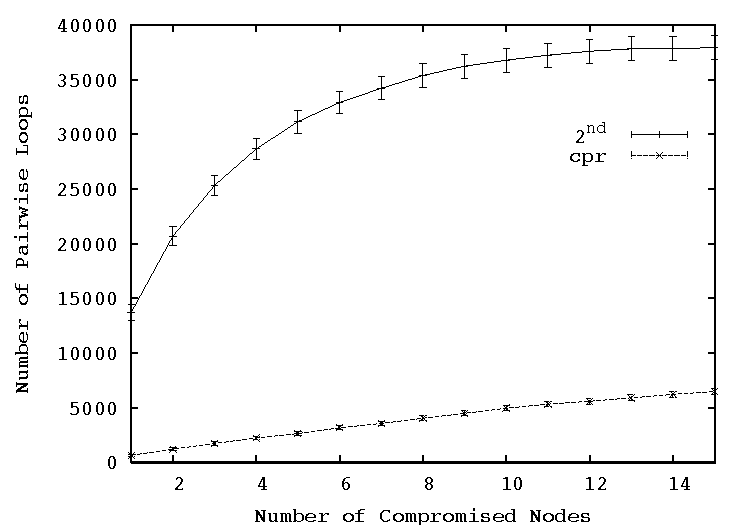
\includegraphics[width=0.32\textwidth]{figs/synch/loops-rand.pdf}}
\subfigure[{Number of Effected Least Cost Paths}]{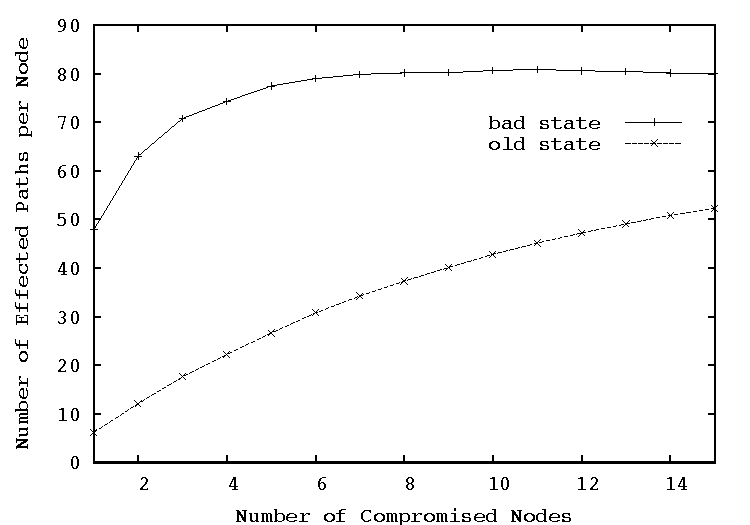
\includegraphics[width=0.32\textwidth]{figs/synch/initial-rand.pdf}}
\caption{Experiment 4 - multiple compromised nodes over \er graphs with link weights selected uniformly at random from $[1,100]$, $p=.05$, $n=100$, and diameter=$6.14$.}
\label{fig:many}
\end{figure*}

\subsubsection{Experiment 5 - Poison Reverse}
%Here we study the benefits of using poison reverse to \second and \cprs. 
We repeat Experiments 2, 3, and 4 using poison reverse for \second and \cprs.  
We do not apply poison reverse to \purge because no routing loops (resulting from the removal of \bads)
exist during \purges's recovery. Additionally, we do not repeat Experiment 1 using poison reverse because we observed few routing loops in that experiment. 

First, we repeat Experiment 2 using poison reverse. The results are shown for one representative topology in Figure \ref{fig:pr-fix}(a),
where \second + {\tt pr} and \cpr + {\tt pr} refer to each respective algorithm
using poison reverse. % The results are consistent for the other topologies considered in Experiments 2 and 3. %\er graphs with other $p$ values and for Internet-like topologies. 

\cpr + {\tt pr} has modest gains over standard \cpr because few routing loops occur with \cprs. On other hand,
\second + {\tt pr} sees a significant decrease in message overhead when compared to the standard \second algorithm because poison reverse removes the many pairwise routing 
loops that occur during \second recovery. However,  \second + {\tt pr} still performs worse than \cpr + {\tt pr} and \purges.  When compared to \cpr + {\tt pr}, 
the same reasons described in Experiment 2 account for \second + {\tt pr}'s poor performance. %high message complexity.  %reverse does not remove routing loops larger than $2$. 
Comparing \purge and \second + {\tt pr} yields interesting insights into the two different approaches for eliminating routing loops: \purge prevents routing loops using diffusing computations
and \second + {\tt pr} uses poison reverse.
Because \purge has lower message complexity than \second + {\tt pr} and poison reverse only eliminates pairwise routing loops, 
it suggests that \purge removes routing loops larger than $2$.
We are currently investigating this claim.

Repeating Experiment 3 using poison reverse yields the same trends as repeating Experiment 2 with poison reverse.  Finally, we consider poison reverse in the case 
of multiple compromised nodes (e.g., we repeat Experiment 4). \second + {\tt pr} and \cpr + {\tt pr} over \er graphs with unit link weights perform only slightly 
better than the basic version of each algorithm, respectively.  This is expected because few pairwise routing loops occur in this scenario.  

Like the single compromised node scenario, in the case of multiple compromised nodes, \second + {\tt pr} and \cpr + {\tt pr} over \er graphs with random link weights provide 
significant improvements over the basic version of each algorithm.  Particularly for \seconds, we observed many pairwise loops in Experiment 4 (Figure \ref{fig:many}(b)). This 
accounts for the effectiveness of poison reverse in this experiment.  Despite the significant improvements, \second + {\tt pr} still performs worse than \cpr + {\tt pr} and \purges. 
\cpr + {\tt pr} performs best among all the recovery algorithms because, as we have discussed, rolling back to a network-wide checkpoint is more efficient than using distance vector's
iterative procedure. Furthermore, poison reverse helps \cpr + {\tt pr} reduce the \infinity problem, improving \cprs's effectiveness in the face of multiple 
compromised nodes. 


\begin{figure*}[t]
\centering
%\subfigure[{Experiment 1}]{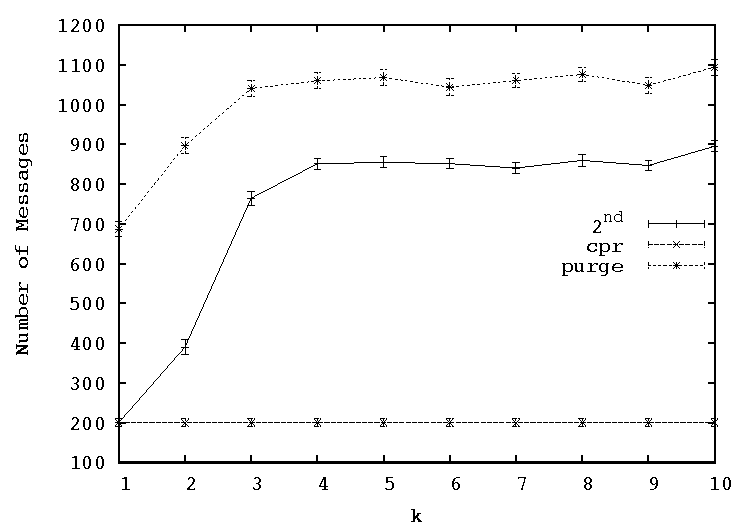
\includegraphics[scale=0.47]{figs/synch/msg5.pdf}}
%\subfigure[{Experiment 2 and 4}]{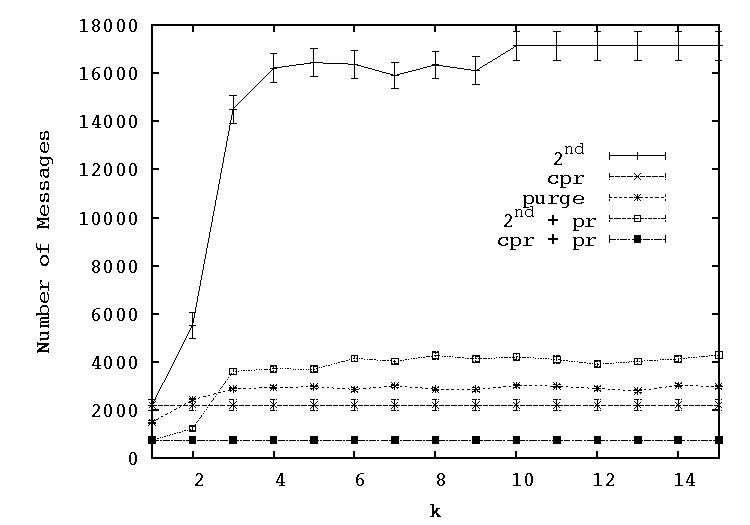
\includegraphics[scale=0.48]{figs/synch/msg-rand-pr5.pdf}}
%\subfigure[{Experiment 1}]{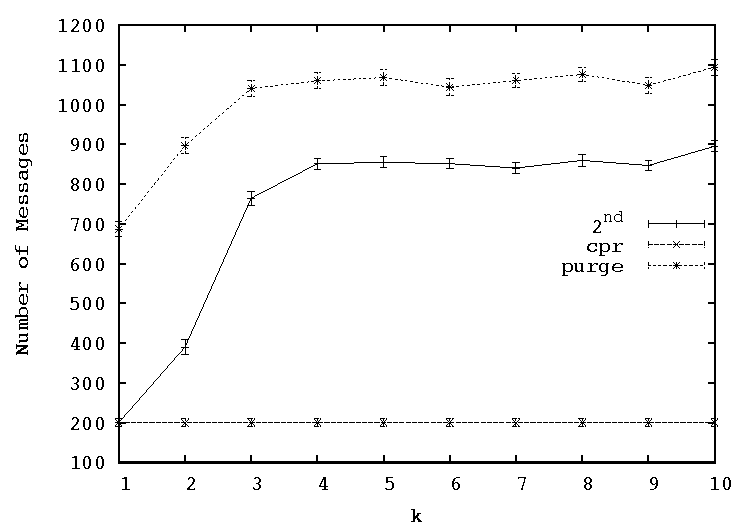
\includegraphics[width=0.49\textwidth]{figs/synch/msg5.pdf}}
\subfigure[{Single Compromised Node}]{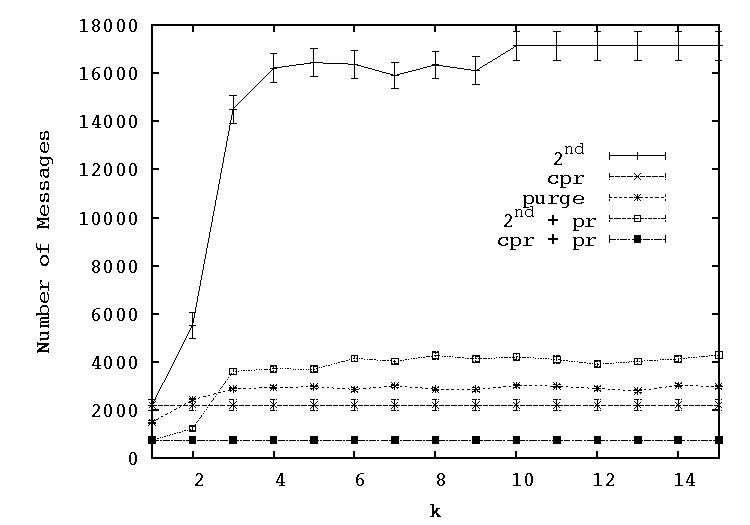
\includegraphics[width=0.32\textwidth]{figs/synch/msg-rand-pr5.pdf}}
\subfigure[{Multiple Compromised nodes}]{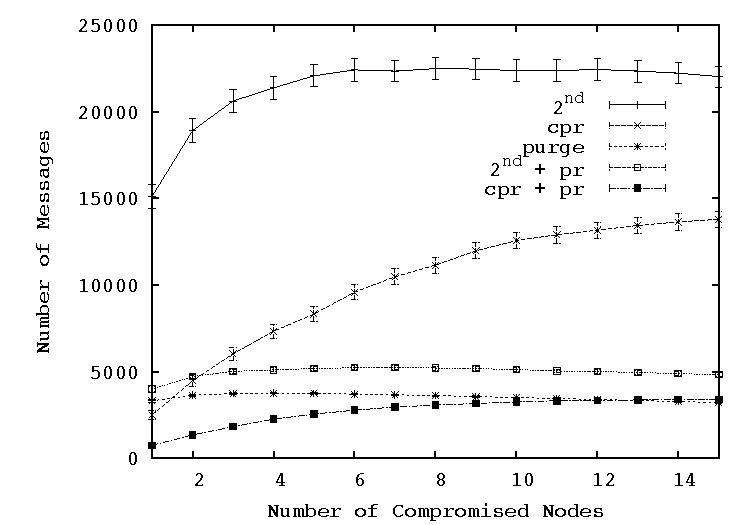
\includegraphics[width=0.32\textwidth]{figs/synch/many-pr-rand5.pdf}}
\caption{Experiment 5 plots.  Algorithms run over \er graphs with random link weights, $n=100$, $p=.05$, and average diameter=$6.14$. 
\second + {\tt pr} refers to \second using poison reverse. Likewise, \cpr + {\tt pr} is \cpr using poison reverse.}
\label{fig:pr-fix}
\end{figure*}




\subsection{Link Weight Change Experiments}
\label{subsec:change}

So far, we have evaluated our algorithms over different topologies with fixed link costs in scenarios with single and multiple compromised nodes.
We found that \cpr using poison reverse outperforms the other algorithms because \cpr removes false
routing state with a single diffusing computation, rather than using an iterative distance vector process as in \second and \purges, and poison reverse removes
all pairwise routing loops that occur during \cpr recovery. 

In the next three experiments we evaluate our algorithms over graphs with changing link costs. We introduce link cost changes between the time \bad is compromised and when \bad is discovered 
(e.g., during $[t',t_b]$). 
In particular, let there be $\lambda$ link cost changes per timestep, where $\lambda$ is deterministic. 
To create a link cost change event, we choose a link (except for all $(v,\bar{v})$ links) whose link will change equiprobably among all links. 
The new link cost is selected uniformly at random from $[1,n]$. 

\subsubsection{Experiment 6 - Link Cost Changes}

Except for $\lambda$, our experimental setup is identical to the one in Experiment 2. We let $\lambda = \{1,4,8\}$. In order to isolate the effects of link costs changes,
we assume that \cpr checkpoints at each timestep.

Figure \ref{fig:lc} shows \purge yields the lowest message overhead for $p=.05$, but only slightly lower than \cprs. 
\cprs's message overhead increases with larger $k$ because there are more link cost change events to process. After \cpr rolls back, it must process all link cost
changes that occurred in $[t',t_b]$. 
In contrast, \second and \purge process some of the link cost change events during the interval $[t',t_b]$ as part of normal distance vector execution. 
In our experimental setup, these messages are not counted because 
they do not occur in Step 4 (i.e., as part of the recovery process) of our simulation scenario described in Section \ref{sec:eval}.

Our analysis further indicates that \second performance suffers because of the \infinity problem. %\purge and \second must 
The gap between \second and the other algorithms shrinks as $\lambda$ increases because as $\lambda$ increases, link cost changes have a larger effect on message overhead.


\begin{figure*}[t]
\centering
\subfigure[{$p=0.05$, diameter=$6.14, \lambda=1$}]{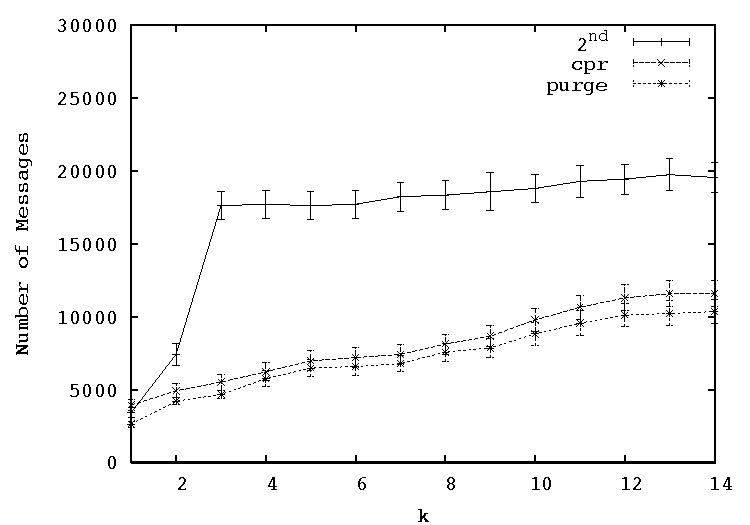
\includegraphics[width=0.32\textwidth]{figs/synch/p05-lc1.pdf}}
%\subfigure[{$p=0.05$, diameter=$6.14, \lambda=2$}]{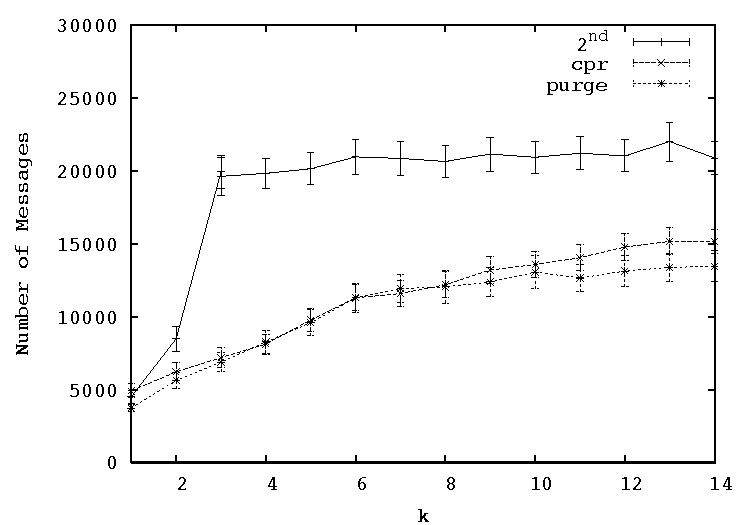
\includegraphics[width=0.32\textwidth]{figs/synch/p05-lc2.pdf}}
\subfigure[{$p=0.05$, diameter=$6.14,\lambda=4$}]{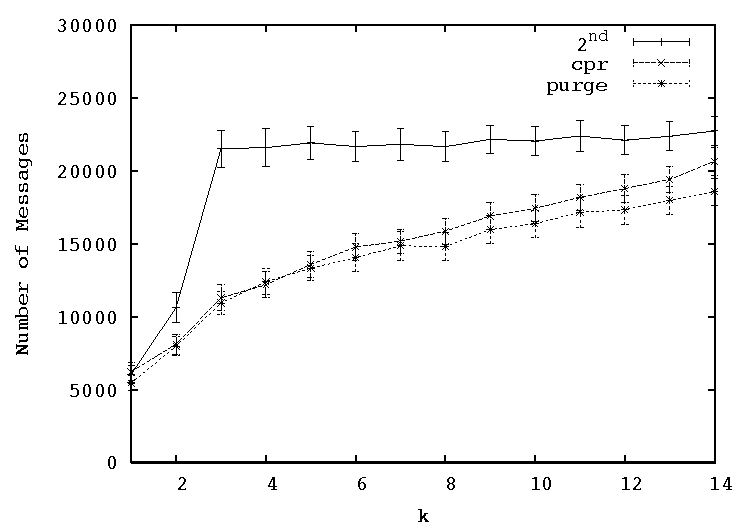
\includegraphics[width=0.32\textwidth]{figs/synch/p05-lc4.pdf}}
\subfigure[{$p=0.05$, diameter=$6.14, \lambda=8$}]{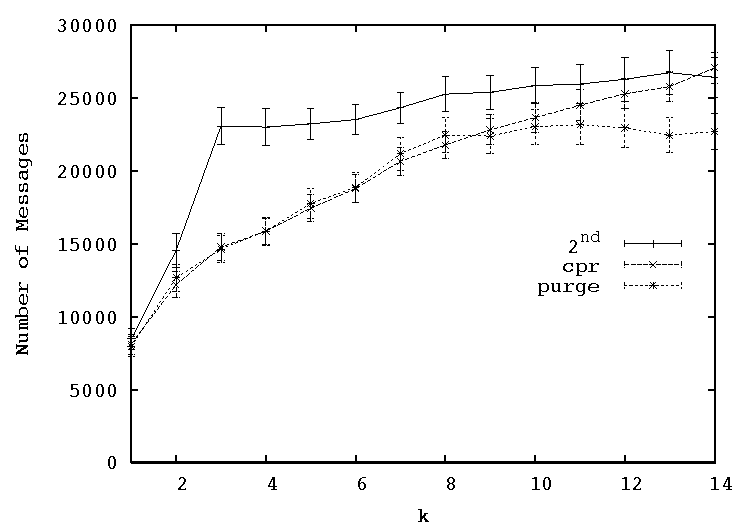
\includegraphics[width=0.32\textwidth]{figs/synch/p05-lc8.pdf}}
\subfigure[{$p=0.15$, diameter=$3.01, \lambda=1$}]{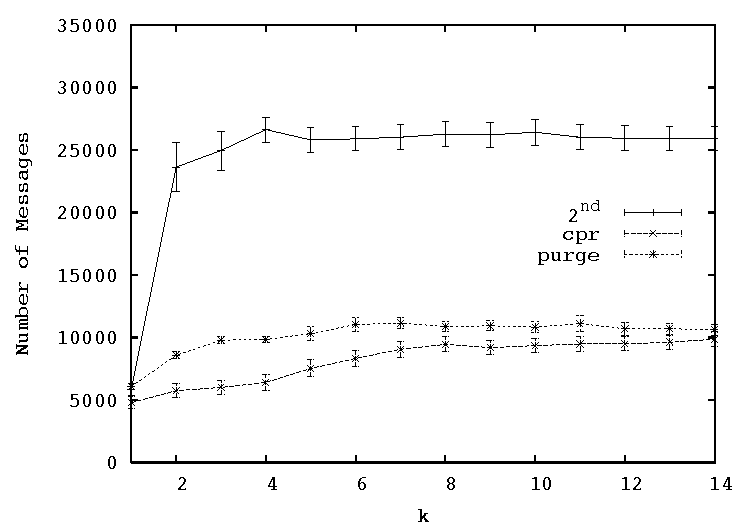
\includegraphics[width=0.32\textwidth]{figs/synch/p15-lc1.pdf}}
\subfigure[{$p=0.15$, diameter=$3.01,\lambda=4$}]{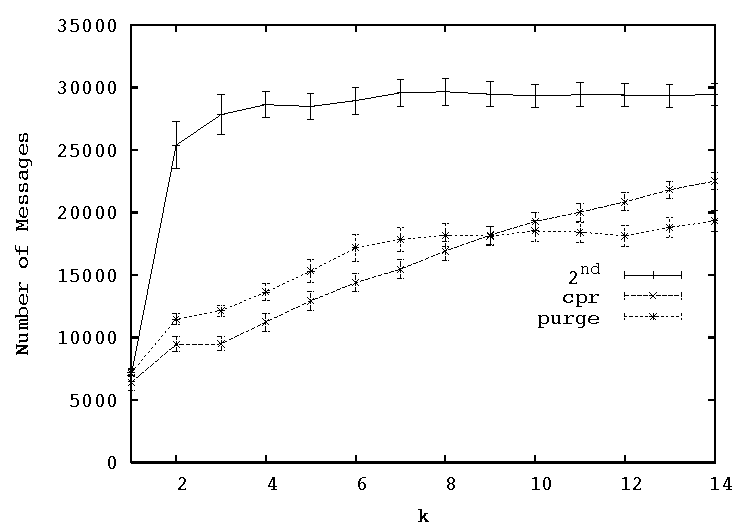
\includegraphics[width=0.32\textwidth]{figs/synch/p15-lc4.pdf}}
\subfigure[{$p=0.15$, diameter=$3.01, \lambda=8$}]{\includegraphics[width=0.32\textwidth]{figs/synch/p15-lc8.pdf}}
%\subfigure[{Cumulative path cost decreases during the simulation}]{\includegraphics[width=0.49\textwidth]{figs/tsdecrease6.pdf}}
\caption{Experiment 6: Message overhead for $p=\{0.05,0.15\}$ \er with link weights selected uniformly random with different $\lambda$ values.}
\label{fig:lc}
\end{figure*}

%\begin{figure*}[t]
%\centering
%\subfigure[{$p=0.15$, diameter=$3.01, \lambda=1$}]{\includegraphics[width=0.32\textwidth]{figs/synch/p15-lc1.pdf}}
%\subfigure[{$p=0.15$, diameter=$3.01,\lambda=4$}]{\includegraphics[width=0.32\textwidth]{figs/synch/p15-lc4.pdf}}
%\subfigure[{$p=0.15$, diameter=$3.01, \lambda=8$}]{\includegraphics[width=0.32\textwidth]{figs/synch/p15-lc8.pdf}}
%\subfigure[{Cumulative path cost decreases during the simulation}]{\includegraphics[width=0.49\textwidth]{figs/tsdecrease6.pdf}}
%\caption{Message overhead for $p=0.15$ \er with link weights selected uniformly random with different $\lambda$ values.}
%\label{fig:lc-p15}
%\end{figure*} 

With larger $p$ values, $\lambda$ has a smaller effect on message complexity because more alternate paths are available. Thus when $p=0.15$ and $\lambda=1$,
most of \purges's recovery effort is towards removing \badvector state, rather than processing link cost changes.  Because
\cpr removes \badvector using a single diffusing computation and there are few link cost changes, \cpr has lower message overhead than \purge in this case. 
As $\lambda$ increases, \cpr has higher message overhead than \purges: there are more link cost changes to process and \cpr must process all such link cost changes, 
while \purge processes some link cost changes during the interval $[t',t_b]$ as part of normal distance vector execution. 

\subsubsection{Experiment 7 - Poison Reverse and Link Cost Changes}
In this experiment, we apply poison reverse to each algorithm and repeat Experiment 6. Because \purges's diffusing computations only eliminate routing loops corresponding 
to \badvector state, \purge is vulnerable to routing loops stemming from link cost changes.  Thus, contrary to Experiment 5, poison reverse improves \purge performance.
The results are shown in Figure \ref{fig:prlc}. Each algorithm using poison reverse has label ``{\tt algorithm-name}'' + {\tt pr}).
Results for different $p$ values yield the same trends. 

All three algorithms using poison reverse show remarkable performance gains.
As confirmed by our profiling numbers, the improvements are significant because routing loops are more pervasive when link costs change.  
Accordingly, the poison reverse optimization yields greater benefits as $\lambda$ increases. % because larger $\lambda$ result in more routing loops. %for the standard \second and \cpr algorithms.

%Each algorithm using poison reverse is vulnerable to routing loops larger than $2$ that originate from link cost changes,
As in Experiment 5, we believe that for \badvector state \emph{only}, \purge + {\tt pr} removes routing loops larger than $2$ while \second + {\tt pr} does not. 
For this reason, we believe that \purge + {\tt pr} performs better than \second + {\tt pr}.  We are currently investigating this claim.
%As in Experiment 3, \second + {\tt pr} performs worse than \purge + {\tt pr} because we believe that for \badvector state \emph{only},
%\purge + {\tt pr} removes routing loops larger than $2$ while \second + {\tt pr} does not. Meanwhile, both 
% \second + {\tt pr} and \purge + {\tt pr} use poison reverse to address routing loops resulting from link cost changes.  Thus both algorithms (and \cpr + {\tt pr})
%are equally vulnerable to routing loops  larger than $2$ originating from link cost changes.
\cpr + {\tt pr} has the lowest message complexity. %among the three algorithms. 
In this experiment, the benefits of rolling back to a global snapshot taken before \bad was compromised outweigh the message overhead required to update stale state pertaining to 
link cost changes that occurred during $[t',t_b]$. As $\lambda$ increases,
the performance gap decreases because \cpr + {\tt pr} must process all link cost changes that occurred in $[t',t_b]$ while \second + {\tt pr}  and \purge + {\tt pr}
process some link cost change events during $[t',t_b]$ as part of normal distance vector execution.

%However, we make the strong performance of \cpr + {\tt pr} comes wiHh
However, \cpr + {\tt pr} only achieves such strong results by making two optimistic assumptions:  we assume perfectly synchronized clocks and checkpointing occurs at each timestep.
In the next experiment we relax the checkpointing assumption.
%However, we make two optimistic assumptions in order to achieve such favorable results for \cpr + {\tt pr}: we assume clocks are perfectly synchronized and checkpointing occurs at each timestep.
%In the next experiment we relax the checkpoint assumption.


\begin{figure*}[t]
\centering
\subfigure[{$p=0.05$, $\lambda=1$}]{\includegraphics[width=0.32\textwidth]{figs/synch/pr-p05-lc1.pdf}}
%\subfigure[{$p=0.05, \lambda=2$}]{\includegraphics[width=0.49\textwidth]{figs/synch/p05-lc2.pdf}}
\subfigure[{$p=0.05$, $\lambda=4$}]{\includegraphics[width=0.32\textwidth]{figs/synch/pr-p05-lc4.pdf}}
\subfigure[{$p=0.05$, $\lambda=8$}]{\includegraphics[width=0.32\textwidth]{figs/synch/pr-p05-lc8.pdf}}
%\subfigure[{Cumulative path cost decreases during the simulation}]{\includegraphics[width=0.49\textwidth]{figs/tsdecrease6.pdf}}
\caption{Plots for Experiment 7. Each figure shows message overhead for \er graphs with link weights selected uniformly at random, $p=0.05$, average diameter is $6.14$, and $\lambda=\{1,4,8\}$.
The curves for \second + {\tt pr}, \purge + {\tt pr}, and \cpr + {\tt pr} refer to each algorithm using poison reverse, respectively.
} 
\label{fig:prlc}
\end{figure*}


\subsubsection{Experiment 8 - Vary Checkpoint Frequency}

In this experiment we study the trade-off between message overhead and storage overhead for \cprs. To this end, we vary the frequency at which \cpr checkpoints and fix 
the interval $[t',t_b]$. Otherwise, our experimental setup is the same as Experiment 6.

Figure \ref{fig:lc-fixk} shows the results for an \er graph with link weights selected uniformly at random between $[1,n]$,
$n=100$, $p=.05$, $\lambda=\{1,4,8\}$ and $k=2$. We plot message overhead against the number of timesteps \cpr must rollback, $z$. \cprs's message overhead increases with larger $z$ 
because as $z$ increases there are more link cost change events to process. \second and \purge have constant message overhead because they operate independent of $z$.

We conclude that as the frequency of \cpr snapshots decreases, \cpr incurs higher message overhead.  Therefore, when choosing the frequency of checkpoints,
the trade-off between storage and message overhead must be carefully considered. 



\begin{figure*}[t]
\centering
\subfigure[{$p=0.05$, $k=2, \lambda=1$}]{\includegraphics[width=0.32\textwidth]{figs/synch/p05-k1.pdf}}
\subfigure[{$p=0.05$, $k=2, \lambda=4$}]{\includegraphics[width=0.32\textwidth]{figs/synch/p05-k4.pdf}}
\subfigure[{$p=0.05$, $k=2, \lambda=8$}]{\includegraphics[width=0.32\textwidth]{figs/synch/p05-k8.pdf}}
%\subfigure[{Cumulative path cost decreases during the simulation}]{\includegraphics[width=0.49\textwidth]{figs/tsdecrease6.pdf}}
\caption{Experiment 8: message overhead for $p=0.05$ \er with link weights selected uniformly random with different $\lambda$ values. $z$ refers to the number of timesteps \cpr must 
rollback. Note the y-axis have different scales.}
\label{fig:lc-fixk}
\end{figure*} 


\subsection{Summary}
\label{subsec:discuss}


Our results show \cpr using poison reverse yields the lowest message and time overhead in all scenarios. \cpr benefits from removing false state with a single
diffusing computation. Also, applying poison reverse significantly reduces \cpr message complexity by eliminating pairwise routing loops resulting from
link cost changes. However, \cpr has storage overhead, requires loosely synchronized clocks, and requires the time \bad was compromised.

\seconds's performance is determined by the \infinity problem. In the case of \er graphs with fixed unit link weights, the \infinity problem was minimal, 
helping \second perform better than \purges. % In all other scenarios, poison reverse significantly improves \second performance because routing loops are pervasive.
For all other topologies, poison reverse significantly improves \second performance because routing loops are pervasive.
Still, \second using poison reverse is not as efficient as \cpr and \purge using poison reverse.

In cases where link costs change, we found that \purge using poison reverse is only slightly worse than \cpr + {\tt pr}. % with poison reverse. 
Unlike \cprs, \purge makes use of computations that follow the injection of false state, that do not depend on false routing state.  
Because \purge does not make the assumptions that \cpr requires, \purge using poison reverse is a suitable alternative for topologies with link cost changes.
%In contrast to \cprs, \purge makes no assumptions 
%other than the identification of \bads, making \purge a suitable algorithm for topologies with link cost changes.

%\purge avoids the \infinity problem by first globally invalidating false state.  Therefore in cases where the \infinity problem is 
%significant, \purge outperforms \seconds.

%When considering graphs with changing link costs, \cprs's performance suffers because it must process all valid link cost changes that occurred since \bad was compromised.
%Meanwhile, \second and \purge make use of computations that followed the injection of false state, that do not depend on false routing state. However, \seconds's performance degrades 
%because of the \infinity problem.  \purge eliminates the \infinity problem and therefore yields the best performance over topologies with changing link costs.

Finally, we found that an additional challenge with \cpr is setting the parameter which determines checkpoint frequency.
Frequent checkpointing yields lower message and time overhead at the cost of more storage overhead. Ultimately, application-specific factors must be considered
when setting this parameter. 


\section{Related Work}
\label{sec:related-pmu}

\full is well-studied \cite{Baldwin93,Brueni05,Haynes02, Mili90, Xu04}.  
Haynes et al. \cite{Haynes02} and Brueni and Heath \cite{Brueni05} both prove \full is NPC.  
However, their proofs make the unrealistic assumption that all nodes are zero-injection.  We drop this assumption and thereby generalize their NPC results for \fulls.
Additionally, we leverage the proof technique from Brueni and Heath \cite{Brueni05} in all four of our NPC proofs, although our proofs
differ considerably in their details. 

%The power systems literature generally ignores the fact that PMUP is NP-Complete because, in practice, power system graphs are small enough to allow for an exact solution to be found.
In the power systems literature, Xu and Abur \cite{Xu04,Xu05} use integer programming to solve \fulls, while Baldwin et al. \cite{Baldwin93} and Mili et al. \cite{Mili90} use simulated annealing 
to solve the same problem. All of these works allow nodes to be either zero-injection or non-zero-injection.  However,
these papers make no mention that \full is NPC, i.e., they do not characterize the fundamental complexity of the problem. 
%The work of Xu and Abur \cite{Xu04} and Phadke et al. are representive of the power systems approach to the problem: formulate the problem as integer 
%program and use an integer programming solver to find the optimal PMU placement.  

Aazami and Stilp \cite{Aazami07} investigate approximation algorithms for \fulls.  They derive a hardness approximation threshold of $2^{\log^{1 -\epsilon}n}$.
Also they prove that in the worst case, {\tt greedy} from Section \ref{sec:approx} does no better $\Theta(n)$ of the optimal solution.  However, this approximation ratio assumes that 
all nodes are zero-injection.
%We leverage this approximation result in proving the approximation ratios of our heuristic-based algorithms.

Chen and Abur \cite{Abur06} and Vanfretti et al. \cite{Vanfretti10} both study the problem of bad PMU data. Chen and Abur \cite{Abur06} formulate their problem differently than \xval and \xvalparts.  
They consider fully observed graphs and add PMUs to the system to make all existing PMU measurements non-critical 
(a critical measurement is one in which the removal of a PMU makes the system
no longer fully observable). Vanfretti et al. \cite{Vanfretti10} define the cross-validation rules used in this paper.  They also derive a
lower bound on the number of PMUs needed to ensure all PMUs are cross-validated and the system is fully observable. 




\section{Conclusions and Future Work}
\label{sec:future}

In this chapter, we developed methods for recovery in scenarios where a malicious node injects false state into a distributed system.  
We studied an instance of this problem in distance vector routing.
We presented and evaluated three new algorithms for recovery in such scenarios. %from false state in distance vector routing 
Among our three algorithms, our results show that \cpr -- a checkpoint-rollback based algorithm -- yields the lowest message and time overhead over topologies
with fixed link costs.  However, \cpr has storage overhead and requires loosely synchronized clocks.
In the case of topologies with changing link costs, \purge performs best by avoiding the problems that plague \cpr and \seconds.
Unlike \cprs, \purge has no stale state to update because \purge does not rollback in time.  
The \infinity problem results in high message overhead for \seconds, while \purge eliminates the \infinity problem by globally purging false state before finding new least cost paths.

As future work, we are interested in finding the worst possible false state a compromised node can inject.  Some options include the minimum distance to all nodes (e.g., 
our choice for false state used in this paper), state that maximizes the effect of the \infinity problem, and false state that contaminates a bottleneck link. 




%\chapter{??? Background: Smart Grid and PMU Sensors ???}



\chapter{PMU Sensor Placement for Measurement Error Detection in the Smart Grid}
\label{ch:pmu}

\section{Introduction}
\label{sec:intro-pmu}

\begin{framed}
\xxxxn{TODO Notes from Proposal Defense:}
\begin{itemize}
        \item \xxxxn{Lixin: Approximation bounds using modularity/sub-modular functions.  } 
	
	\item \xxxxn{Lixin: mention in future work (may already do this) that with special topologies you may be able to find more efficient algorithms for PMU placement.}

	\item \xxxxn{State Aazami et al show that the approximation for greedy algorithm is $\Theta(n)$, under the assumption that all nodes are zero-injection.  }
\end{itemize}
\end{framed}
               


This chapter considers placing electric power grid sensors, called phasor measurement units (PMUs), to enable measurement error detection.
%\xx{move paragraph to Smart Grid Overview Chapterr}
Significant investments have been made to deploy PMUs on electric power grids worldwide. PMUs provide \emph{synchronized} voltage and current measurements at a sampling rate orders 
of magnitude higher than the status quo: $10$ to $60$ samples per second rather than one sample every $1$ to $4$ seconds.  This allows system operators to directly measure the state of the electric power grid in real-time, rather than 
relying on imprecise state estimation. Consequently, PMUs have the potential to enable
an entirely new set of applications for the power grid:  protection and control during abnormal conditions, real-time distributed control, postmortem analysis of system faults,
advanced state estimators for system monitoring, and the reliable integration of renewable energy resources \cite{Naspi10}.

%\xx{move paragraph to Smart Grid Overview Chapter}
An electric power system consists of a set of buses  -- electric substations, power generation centers, or aggregation points of electrical loads -- and transmission lines connecting those buses.
The state of a power system is defined by the voltage phasor -- the magnitude and phase angle of electrical sine waves -- of all system buses and the current phasor of all transmission lines.
PMUs placed on buses provide real-time measurements of these system variables.
However, because PMUs are expensive, they cannot be deployed on all system buses \cite{Baldwin93}\cite{LaRee10}. Fortunately, the voltage phasor at a system bus can, at times, 
be determined (termed {\it observed} in this thesis) even when a PMU is not placed at that bus, by applying Ohm's and Kirchhoff's laws
on the measurements taken by a PMU placed at some nearby system bus \cite{Baldwin93}\cite{Brueni05}. Specifically, with correct placement of enough PMUs at a subset of system buses, the entire system state can be determined. 

In this chapter, we study two sets of PMU placement problems.  The first problem set consists of \full and \maxincs, and considers maximizing the observability of the network via PMU placement. \full considers the minimum number of PMUs needed 
to observe all system buses, while \maxinc considers the maximum number of buses that can be observed with a given number of PMUs. 
A bus is said to be {\em observed} if there is a PMU placed at it or if
its voltage phasor can be calculated using Ohm's or Kirchhoff's Law.  Although \full is well studied \cite{Baldwin93,Brueni05,Haynes02,Mili90,Xu04}, existing work considers only networks consisting solely of zero-injection buses, 
an unrealistic assumption in practice,
while we generalize the problem formulation to include mixtures of zero and  non-zero-injection buses. Additionally, our approach for analyzing \full provides the foundation with which to present the other three new (but related) PMU placement problems.

The second set of placement problems considers PMU placements that support PMU error detection. PMU measurement errors have been recorded in actual systems \cite{Vanfretti10}. 
One method of detecting these errors is to deploy PMUs ``near'' each other, thus enabling them to {\em cross-validate} each-other's measurements. 
{\xvals} aims to minimize the number of PMUs needed to observe all buses while insuring PMU cross-validation, and {\xvalparts} computes the maximum number of observed buses for a given number of PMUs, while insuring PMU cross-validation.


We make the following contributions in this chapter: 
\begin{itemize}
    
	\item We formulate two PMU placement problems, which (broadly) aim at maximizing observed buses while minimizing the number of PMUs used. Our formulation extends previously studied systems by 
	considering both zero and non-zero-injection buses.

    \item We formally define graph-theoretic rules for PMU cross-validation. Using these rules, we formulate two additional PMU placement problems that seek to maximize 
	the number of observed buses while minimizing the number of PMUs used under the condition that the PMUs are cross-validated. 

    \item We prove that all four PMU placement problems are NP-Complete. This represents our most important contribution.

	\item Given the proven complexity of these problems, we evaluate heuristic approaches for solving these problems. For each problem, we describe a greedy algorithm, and prove that each greedy
	algorithm has polynomial running time.

	\item Using simulations, we evaluate the performance of our greedy approximation algorithms over synthetic and actual
	IEEE bus systems. We find that the greedy algorithms yield a PMU placement that is, on average, within $97\%$ optimal. Additionally, we find that 
	the cross-validation constraints have limited effects on observability: on average our greedy algorithm that places PMUs according to the cross-validation rules observes 
	only $5.7\%$ fewer nodes than the same algorithm that does not consider cross-validation.

\end{itemize}

The rest of this chapter is organized as follows. In Section \ref{sec:prelim} we introduce our modeling assumptions, notation, and observability and cross-validation rules. In Section \ref{sec:problem-analysis} we formulate and prove the complexity of our four PMU placement problems. Section \ref{sec:approx} presents the approximation algorithms for each problem and Section \ref{sec:simulations} considers our simulation-based evaluation. We conclude with a review of related work (Section \ref{sec:related-pmu}) 
and concluding remarks (Section \ref{sec:pmu-conclude}).


\section{Preliminaries}
\label{sec:prelim}

In this section we introduce notation and underlying assumptions (Section \ref{subsec:notation-assume}), 
and define our observability (Section \ref{subsec:observe}) and cross-validation (Section \ref{subsec:xval-rules}) rules.

%Before starting our analysis, we detail the notation used in this document.

\subsection{Assumptions, Notation, and Terminology}
\label{subsec:notation-assume}

%Consistent with the conventions in \cite{Baldwin93,Brueni05,Abur06,Mili90,Xu04,Xu05}, we make the following two assumptions about PMU placements and buses. First, a PMU can only be placed on a bus.
%Second, a PMU on a bus measures the voltage phasor at the bus and the current phasor of all transmission lines connected to it. 

Consistent with the conventions in \cite{Baldwin93,Brueni05,Abur06,Mili90,Xu04,Xu05}, we make the following assumptions about PMU placements and buses. 
First, a PMU can only be placed on a bus.  Second, a PMU on a bus measures the voltage phasor at the bus and the current phasor of all transmission lines connected to it.

%\begin{enumerate}
%	\item A PMU can only be placed on a bus.
%	\item A PMU on a bus measures the voltage phasor at the bus and the current phasor of all transmission lines connected to it. 
%\end{enumerate}

We model a power grid as an undirected graph $G=(V,E)$.  Each $v \in V$ represents a bus.  A bus is either an electrical substation, a power generation center, or an 
aggregation of loads. $V=V_Z \cup V_I$, where $V_Z$ is the set of all zero-injection buses and $V_I$ is the set of all non-zero-injection buses.  A bus is zero-injection if it has no load nor generator \cite{Zhang10}.
All other buses are non-zero-injection.  For simplicity, we refer to non-zero-injection buses as injection buses in the remainder of the paper. 
Each $(u,v) \in E$ is a transmission line connecting buses $u$ and $v$.  Figure \ref{fig:example} is an example of a power system modeled as such an undirected graph.

\begin{figure}[t]
\centering
\includegraphics[scale=0.51]{figs/example4.pdf}
%\includegraphics[scale=0.51]{figs/example2.pdf}
\caption{Example power system graph. PMU nodes ($a,b$) are indicated with darker shading. Injection nodes have solid borders while zero-injection nodes  ($g$) have dashed borders.}
\label{fig:example}
\end{figure}

Using the same notation as Brueni and Heath \cite{Brueni05}, we define two $\Gamma$ functions. For $v\in V$ let $\Gamma(v)$ be the set of $v$'s neighbors in $G$, and $\Gamma[v] = \Gamma(v)\cup \{v\}$. 
% Since neighbor relationships are symmetric, $u\in\Gamma(v)\Rightleftarrow v\in\Gamma(u)$. 
A PMU placement $\Phi_G \subseteq V$ is a set of nodes at which PMUs are placed,
%We use the definition of a PMU placement from Brueni and Heath \cite{Brueni05}: a PMU cover, $\Phi$, is a subset of $V$ in which PMUs are placed such that all $v \in V$ and all $(u,v) \in E$ observed.
and $\Phi^R_G\subseteq V$ is the set of observed nodes for graph $G$ with placement $\Phi_G$ (see definition of observability below). %For convenience, we let $\Phi^R$ represent the observed nodes for graph $G$.
$k^* = \min \{|\Phi_G|:\Phi^R_G=V\}$ denotes the minimum number of PMUs needed to observe the entire network. Where the graph $G$ is clear from the context, we drop the $G$ subscript.
%Finally, $m$ is a constant corresponding to a graph $G=(V,E)$ such that $m < |V|$. 

%We let $\Phi^-$ represent the observed edges and $\Phi^R$ represent the observed nodes.
%All notation used in this document is shown in Table \ref{tab:notation}.

For convenience, we refer to any node with a PMU as a \emph{PMU node}. Additionally, for a given PMU placement we say that set $W\subseteq V$ is observed if all nodes in $W$ are observed, and if $W=V$ we refer to the graph as \emph{fully observed}. 


%%%%%%%%%%%%%%%%%%%%%%%%%%%%%%%%%%%%%%%%%%%%%%%%%%%%%%%%%%%%%%%%%%%% BEGIN COMMENT %%%%%%%%%%%%%%%%%%%%%%%%%%%%%%%%%%%%%%%%%%%%%%%%%%%%%%%%%%%%%%%%%%%%%%%%%%%%%%%%%%%%%%%%%%%%%%%%%%%%%%%%%%%%%%%%
\begin{comment}
\begin{table}[t]
\begin{center}
\begin{tabular}{l l} 
\hline \hline
   	{\bf Notation} & {\bf Meaning} \\
		  \hline 
		  	$G$ &  undirected graph $(V,E)$ where each $v \in V$ is a bus and each \\
				&  $(u,v) \in E$ is a transmission line connecting $u$ and $v$\\
			$\Gamma(v)$ & $\{u \in V$ $|$ $(u,v) \in E \}$ \\ 
			$\Gamma[v]$ & $\Gamma(v) \cup \{v\}$ \\
 		 	$n$ & $|V|$ \\
			$\Phi$ & a subset of $V$ in which PMUs are placed such that all \\ 
				   & $v \in V$ and all $(u,v) \in E$ observed  \\
			$\Phi^R$ & set of observed nodes \\
			$\Phi^-$ & set of observed edges \\
			\hline \hline
	\end{tabular}
	\end{center}
\caption{Notation Table}
\label{tab:notation}
\end{table}
\end{comment}
%%%%%%%%%%%%%%%%%%%%%%%%%%%%%%%%%%%%%%%%%%%%%%%%%%%%%%%%%%%%%%%%%%%% END COMMENT %%%%%%%%%%%%%%%%%%%%%%%%%%%%%%%%%%%%%%%%%%%%%%%%%%%%%%%%%%%%%%%%%%%%%%%%%%%%%%%%%%%%%%%%%%%%%%%%%%%%%%%%%%%%%%%%

\subsection{Observability Rules}
\label{subsec:observe}

We use the simplified observability rules elegantly formulated by Brueni and Heath \cite{Brueni05}.  We restate the rules here:  %which we restate here:  %For completeness, we restate the rules here:
%We use the simplified observability rules elegantly stated by Brueni and Heath \cite{Brueni05}, which we restate here:  %For completeness, we restate the rules here:
\begin{enumerate}
	
	\item {\bf Observability Rule 1 (O1)}.  {\it If node $v$ is a PMU node, then $\Gamma[v]$ is observed. Formally, if $v \in \Phi_G$, then $\Gamma[v] \subseteq \Phi^R_G$. }

	\item {\bf Observability Rule 2 (O2)}. {\it If a zero-injection node, $v$, is observed and  $\Gamma(v)\backslash\{u\}$ is observed for some $u\in\Gamma(v)$, then  $\Gamma[v]$ is observed.
	Formally, if $v \in \Phi^R_G \cap V_Z$ and $|\Gamma(v) \cap (V - \Phi^R_G)| \leq 1$, then $\Gamma[v] \subseteq \Phi^R_G$. }

\end{enumerate}

Consider the example in Figure \ref{fig:example}, where the shaded nodes are PMU nodes and $g$ is the only zero-injection node. 
%{\footnote {\small For all power system graphs shown in this document zero-injection nodes have a dashed border and injection nodes have a solid border.}}
Nodes $a-d$ are observed by applying O1 at the PMU at $a$, and nodes $a,b,f$ and $g$ are observed by applying O1 at $b$. 
$e$ cannot be observed via $c$ because $c$ does not have a PMU (O1 does not apply) and is an injection node (O2 does not apply). % so $e$ cannot be observed via $c$, which is its only neighbor. 
%$c$ does not have a PMU (O1 does not apply) and is an injection node (O2 does not apply), so $e$ cannot be observed via $c$, which is its only neighbor. 
Similarly, $j$ is not observed via $f$. Finally, although $g \in V_Z$, O2 cannot be applied at $g$ because $g$ has two unobserved neighbors $i,h$, so they remain unobserved.

Since O2 only applies with zero-injection nodes, more nodes are likely observed when nodes are zero-injection. For example, consider the case where $c$ and $f$ are {\em zero-injection} nodes. $a-d$, $g$ and $f$ are still observed as before, as O1 makes no 
conditions on the node type. Additionally, 
since $c,f \in V_Z$ and each has a single unobserved neighbor,  we can apply O2 at each of them to observe $e,j$, respectively. % making $e$ and $j$, respectively, observed.   
We evaluate the effect of increasing the number of zero-injection nodes on observability in our simulations (Section \ref{subsec:zero}).

%Finally, O2 can be applied at $e$ because $e \in V_Z$, $e$ is observed, and all of $e$'s neighbors except $i$ are observed. As a result, $i$ becomes observed. 
%Note that O2 cannot be applied at $f$ because $f$ has two unobserved neighbors. %This leaves $g$ and $h$ as the only two unobserved nodes in this example. 

%\begin{figure*}[t]
%  \begin{center}
%    \fbox{\subfigure[Case O1]{\label{fig:s1}\includegraphics[scale=0.28]{figs/s1.pdf}}}
%    \fbox{\subfigure[Case O2]{\label{fig:s2}\includegraphics[scale=0.28]{figs/s2.pdf}}} 
%  \end{center}
%	\caption{Rule Set 2} 
%  \label{fig:ruleset2}
%\end{figure*}




\subsection{Cross-Validation Rules}
\label{subsec:xval-rules}

% If phasor measured by 2 or more PMUs
From Vanfretti et al. \cite{Vanfretti10}, PMU measurements can be cross-validated when: (1) a 
voltage phasor of a non-PMU bus can be computed by PMU data from two different buses or (2) the current phasor of a transmission line can be computed from PMU data from two different buses. 
%Note that Vanfretti et al. \cite{Vanfretti10} use the term ``redundancy'' instead of cross-validation.  
{\footnote {\small  Vanfretti et al. \cite{Vanfretti10} use the term ``redundancy'' instead of cross-validation. }}  
Although it is the PMU data that is actually being cross-validated,
for convenience, we say a PMU is cross-validated. 
A PMU is \emph{cross-validated} if one of the rules below is satisfied \cite{Vanfretti10}: 
\begin{enumerate}
	
	\item {\bf Cross-Validation Rule 1 (XV1)}.  {\it If two PMU nodes are adjacent, then the PMUs cross-validate each other. % (Figure \ref{fig:validate}(a)). 
	Formally, if $u, v \in \Phi_G$, $u \in \Gamma(v)$, then the PMUs at $u$ and $v$ are cross-validated.}

	\item {\bf Cross-Validation Rule 2 (XV2)}. {\it If two PMU nodes have a common neighbor, then the PMUs cross-validate each other. % (Figure \ref{fig:validate}(b)). 
	Formally, if $u, v \in \Phi_G$, $u\neq v$ and $\Gamma(u)\cap\Gamma(v)\neq\emptyset$, then the PMUs at $u$ and $v$ are cross-validated.}
\end{enumerate}
In short, the cross-validation rules require that {\em the PMU is within two hops of another PMU}.
For example, in Figure \ref{fig:example}, the PMUs at $a$ and $b$ cross-validate each other by XV1. 

XV1 derives from the fact that both PMUs are measuring the current phasor of the transmission line connecting the two PMU nodes.  XV2 is more subtle.  
Using the notation specified in XV2, when computing the voltage phasor of an element in $\Gamma(u)\cap\Gamma(v)$ the voltage equations include variables to 
account for measurement error (e.g., angle bias) \cite{Vanfretti-thesis}. %\cite{Vanfretti10}.
When the PMUs are two hops from each other, there are more equations than unknowns, allowing for measurement error detection. 
Otherwise, the number of unknown variables exceeds the number of equations, which eliminates the possibility of detecting measurement errors \cite{Vanfretti-thesis}.
%Otherwise, the number of unknown variables grows faster than the number of equations, which eliminates the possibility of detecting measurement errors \cite{Vanfretti-thesis}.

%XV1 derives from the fact that both PMUs are measuring the current phasor of the transmission line connecting the two PMU nodes.  XV2 is more subtle.
%Using the notation specified in XV2, when computing the voltage phasor of an element in $\Gamma(u)\cap\Gamma(v)$ the equations include variables to account for measurement error (e.g., angle bias).
%%In order to account for measurement error, the equations used to compute the voltage phasor of the neighbor node shared by the PMU nodes include varialbes to account
%%for measurement error. Computing the voltage phasor of the neighbor node shared by the two PMU nodes
%%When computing the voltage phasor of the common neighbor node shared by the PMU nodes the equations include variables to account for measurement error (e.g., angle bias).
%When the PMUs are two hops from each other, there are more equations than unknowns, allowing for measurement error detection.
%Otherwise, the number of unknown variables exceeds the number of equations, which eliminates the possibility of detecting measurement errors \cite{Vanfretti-thesis}.
%Otherwise, the number of unknown variables grows faster than the number of equations, which eliminates the possibility of detecting measurement errors \cite{Vanfretti-thesis}.






\section{Four NP-Complete PMU Placement Problems}
\label{sec:problem-analysis}

In this section we first define four PMU placement problems and then provide a high-level description of the proof strategy we use to prove each problem is NP-Complete.
\yyn{In all four problems defined in this paper, we are only concerned with computing the voltage phasors of each bus (i.e., observing the buses). 
Using the values of the voltage phasors, Ohm's Law can be easily applied to compute the current phasors of each transmission line.}
Also, we consider networks with both injection and zero-injection buses.


\subsection{Problem Statements}

Here we briefly define each of our four PMU placement problems: \fulls, \maxinc, \xvalparts, and \xvals. \\ 
{\bf \full Decision Problem:} \\
\indent \underline{Instance}: Graph $G=(V,E)$ where $V=V_Z \cup V_I$, $V_Z \neq \emptyset$, $k$ PMUs such that $k \geq 1$. \\
\indent \underline{Question}: Is there a $\Phi_G$ such that $|\Phi_G| \leq k$ and $\Phi^R_G = V$?  \\
{\bf \maxinc Decision Problem:} \\
\indent \underline{Instance}: Graph $G=(V,E)$ where $V=V_Z \cup V_I$, $k$ PMUs such that $1 \leq k < k^*$. \\
\indent \underline{Question}: For a given $m< |V|$, is there a $\Phi_G$ such that $|\Phi_G| \leq k$ and $m \leq |\Phi^R_G| < |V|$? \\
{\bf \xval Decision Problem:} \\
\indent \underline{Instance}: Graph $G=(V,E)$ where $V=V_Z \cup V_I$, $k$ PMUs such that $k \geq 1$. \\
\indent \underline{Question}: Is there a $\Phi_G$ such that $|\Phi_G| \leq k$ and $\Phi^R_G = V$ under the condition that each $v \in \Phi_G$ is cross-validated? \\
{\bf \xvalpart Decision Problem:} \\
\indent \underline{Instance}: Graph $G=(V,E)$ where $V=V_Z \cup V_I$, $k$ PMUs such that $1 \leq k < k^*$, and some $m<|V|$. \\
\indent \underline{Question}: Is there a $\Phi_G$ such that $|\Phi_G| \leq k$ and $m \leq|\Phi^R_G| < |V|$ under the condition that each $v \in \Phi_G$ is cross-validated?


\begin{theorem}
\maxincs, \xvalparts, \full and \xval are all NP-Complete.
\label{thm:pmu-npc}
\end{theorem}



\subsection{Overview of NPC Proof Strategy}
\label{subsec:proofstrat}
In this section, we outline the proof strategy we used in each of NP-Completeness proofs.  Due to space constraints we omit the actual NPC proofs. 
Our proofs follow a similar structure proposed by Brueni and Heath \cite{Brueni05}. The authors prove NP-Completeness by reduction from planar 3-SAT (\sats).
A 3-SAT formula, $\phi$, is a boolean formula in conjunctive normal form (CNF) such 
that each clause contains at most $3$ literals. For any 3-SAT formula $\phi$ with the sets of variables $\{v_1,v_2, \dots , v_r\}$ and clauses $\{c_1,c_2, \dots , c_s \}$, $G(\phi)$ 
is the bipartite graph $G(\phi)=(V(\phi),E(\phi))$ defined as follows:
\begin{eqnarray*}
 V(\phi) &= &\{v_i\; \vert\; 1 \leq i \leq r \} \cup \{c_j \;\vert\; 1 \leq j \leq s \} \\
 E(\phi) &=& \{ (v_i,c_j)\;\vert\; v_i \in c_j\;\; or \;\; \overline{v_i} \in c_j\}.
\end{eqnarray*}
Note that edges pass only between $v_i$ and $c_j$ nodes, and so the graph is bipartite.  \sat is a 3-SAT formula such that $G(\phi)$ is planar \cite{Lich82}. 
For example, \sat formula
	 $\varphi = (\overline{v_1} \vee v_2 \vee v_3) \wedge (\overline{v_1} \vee \overline{v_4} \vee v_5) \wedge (\overline{v_2} \vee \overline{v_3} \vee \overline{v_5}) 
	 \wedge (v_3 \vee \overline{v_4}) \wedge  (\overline{v_3} \vee v_4 \vee \overline{v_5})$
has graph $G(\varphi)$ shown in Figure \ref{fig:gvarphi}. 
Discovering a satisfying assignment for  \sat is an NPC problem, and so it can be used in a reduction to prove the complexity of the problems we address here. 

Following the approach in \cite{Brueni05}, for \sat formula, $\phi$, we replace each variable node and each clause node in $G(\phi)$ with a specially constructed set of nodes,
termed a {\em gadget}. In this work, all variable gadgets will have the same structure, and all clause gadgets have the same structure (that is different from the variable gadget structure), 
and we denote the resulting graph as $H(\phi)$. In $H(\phi)$, each {\em variable} gadget has a subset of nodes that semantically represent assigning ``True" to that variable, and a subset of 
nodes that represent assigning it ``False". When a PMU is placed at one of these nodes, this is interpreted as assigning a truth value to the \sat variable corresponding with that gadget. 
Thus, we use the PMU placement to determine a consistent truth value for each \sat variable. Also, clause gadgets are connected to variable gadgets at either ``True" or ``False" (but never both) 
nodes, in such a way that the clause is satisfied if and only if {\em at least one} of those nodes has a PMU.

%While we assume $G(\phi)$ is planar, we make no such claim regarding $H(\phi)$, though in practice all graphs used in our proofs are indeed planar. The proof of NPC rests on the fact that 
%solving the underlying $\phi$ formula is NPC.

While the structure of our proofs is adapted from \cite{Brueni05}, the variable and clause gadgets we use to correspond to the \sat formula are novel, thus leading to a 
different set of proofs. Our work here demonstrates how the work in \cite{Brueni05} can be extended, using new variable and clause gadgets, to address a wide array of PMU placement problems.

\begin{figure}[t]

\subfigure[$G(\varphi)=(V(\varphi),E(\varphi))$ formed from $\varphi$ in Equation (\ref{eqn:varphi}).]{\label{fig:gvarphi}\includegraphics[scale=0.53]{figs/gvarphi.pdf}}
\subfigure[Graph formed using variable gadget from ...]{\label{fig:varphi2}\includegraphics[scale=0.53]{figs/proof1-inject-example.pdf}}

\caption{Example } 
\end{figure}


\begin{figure}[t]
\centering
\includegraphics[scale=0.53]{figs/proof1-inject-example.pdf}
%\includegraphics[scale=0.51]{figs/example2.pdf}
\caption{Graph $G=(V,E)=H_1(\varphi)$ formed from $\varphi$ formula in Theorem \ref{thm:npc-full} proof. Nodes with a dashed border are zero-injection nodes.}
\label{fig:proof1-inject-example}
\end{figure}

\begin{figure}[t]
    \fbox{\subfigure[Variable gadget $V_i$ used in Theorem \ref{thm:npc-full} and Theorem \ref{thm:npc-maxinc}.]
	{\label{fig:diamond-gadget}\includegraphics[scale=0.39]{figs/diamond-gadget.pdf}}}
    \fbox{\subfigure[Clause gadget $C_j$ used in Theorem \ref{thm:npc-maxinc}.]
	{\label{fig:line-gadget}\includegraphics[scale=0.39]{figs/line-gadget.pdf}}}
	\caption{Gadgets used in Theorem \ref{thm:npc-full} and Theorem \ref{thm:npc-maxinc}. $Z_i$ in Figure (a) is the only zero-injection node. The dashed edges in Figure (a) are connections to clause gadgets.  Likewise, the dashed edges in Figure (b) are connections to variable gadgets. }
  \label{fig:pmu-gadgets}
\end{figure}


%\begin{figure}[t]
%\centering
%\includegraphics[scale=0.53]{figs/gvarphi.pdf}
%\caption{$G(\varphi)=(V(\varphi),E(\varphi))$ formed from $\varphi$ in Equation (\ref{eqn:varphi}). }
%\label{fig:gvarphi}
%\end{figure}





\section{Approximation Algorithms}
\label{sec:approx}

Because all four placement problems are NPC, we propose greedy approximation algorithms for each problem, which iteratively add 
a PMU in each step to the node that observes the maximum number of new nodes. We present two such algorithms, one that directly addresses \maxinc ({\tt greedy}) and the other 
\xvalpart ({\tt xvgreedy}). {\tt greedy} and {\tt xvgreedy} can easily be used to solve \full and \xvals, respectively, by selecting the appropriate $k$ value to ensure full observability.
We prove these algorithms have polynomial complexity (i.e., they are in $\mathcal{P}$), making them feasible tools for approximating optimal PMU placement.
Lastly, we explore the possibility that the PMU observability rules are submodular functions (Section \ref{subsec:submodular}).

\subsection{Greedy Approximations}
\label{sec:greedy-approx}

{\bf {\tt greedy} Algorithm}. We start with $\Phi = \emptyset$.  At each iteration, we add a PMU to the node that results in the observation of the maximum number of 
new nodes. The algorithm terminates when all PMUs are placed.  {\footnote {\small The same greedy algorithm is proposed by Aazami and Stilp \cite{Aazami07} and
is shown to  $\Theta(n)$ approximation ratio under the assumption that all nodes are zero-injection.}}
The pseudo-code for {\tt greedy} can be found in Appendix \ref{sec:appendix-approx} (Algorithm \ref{alg:greedy}).

\begin{theorem}
For input graph $G=(V,E)$ and $k$ PMUs {\tt greedy} has $O(dkn^3)$ complexity, where $n=|V|$ and $d$ is the maximum degree node in $V$.
\label{thm:greedy-complex}
\end{theorem}
\begin{proof}
The proof can be found in Appendix \ref{sec:appendix-approx} (Theorem \ref{thm:app-greedy-complex}).
\end{proof}

{\bf {\tt xvgreedy} Algorithm}. {\tt xvgreedy} is almost identical to {\tt greedy}, except that PMUs are added in pairs such that the selected pair observe
the maximum number of nodes under the condition that the PMU pair satisfy one of the cross-validation rules. 
We provide the pseudo code for {\tt xvgreedy} in Algorithm \ref{alg:xvgreedy}.
%We provide the pseudo code for {\tt xvgreedy} and prove that {\tt xvgreedy} has polynomial running time in our Technical Report \cite{Tech12}. 

%Our Technical Report \cite{Tech12} gives the pseudo code for {\tt greedy} and {\tt xvgreedy} and includes proofs
%that these algorithms have polynomial complexity, making them feasible tools for approximating optimal PMU placement. 

%\xxn{Aazami and Stilp prove {\tt greedy} has a $\Theta(n)$ approximation ratio under the assumption that all nodes are zero-injection.}
\begin{theorem}
For input graph $G=(V,E)$ and $k$ PMUs {\tt xvgreedy} has $O(kdn^3)$ complexity, where $n=|V|$ and $d$ is the maximum degree node in $V$.
\label{thm:xvgreedy-complex}
\end{theorem}
\begin{proof}
This theorem is proved in Appendix \ref{sec:appendix-approx} (Theorem \ref{thm:app-xvgreedy-complex}).
\end{proof}


\subsection{Observability Rules as Submodular Functions?}
\label{subsec:submodular}

Submodular functions are set functions with diminishing marginal returns: the value that each subsequent element adds decreases as the size of the input set increases. 
More formally, let $X$ be a ground set such that $|X|=n$. We define a set function on $X$ as $f: 2^X \rightarrow \mathbb{R}$.
Using the definition from Dughmi \cite{Dughmi09} %\footnote{\url{http://theory.stanford.edu/~shaddin/papers/submodular\_survey.pdf}}, %a set function $f: 2^X \rightarrow \mathbb{R}$ 
$f$ is \emph{submodular} if, for all $A,B \subseteq X$ with $A \subseteq B$, and for each $j \in X$,
\begin{eqnarray}
f(A \cup \{j\}) - f(A) &\geq& f(B \cup \{j\}) - f(B)
\end{eqnarray}
It has been shown that greedy algorithms admit a $1-1/e$ approximation of submodular functions \cite{Nem78}, where $e$ is the base of the natural logarithm. For this reason,
we aim to show that our observability rules are submodular.

%For the PMU placement problem, we define $f: 2^X \rightarrow \mathbb{R}$ on graph, $G=(V,E)$, as the number of observed nodes derived by placing a PMU at each $x \in X$.  
For the PMU placement problem, consider $G=(V,E)$.  For $S \subseteq V$ we define $f(S)$ as the number of observed nodes derived by placing a PMU at each $s \in S$.  
We prove that $f$ is not submodular for graphs containing zero-injection nodes (Theorem \ref{thm:submodular1}) but is submodular when restricted
to graphs with only injection nodes (Theorem \ref{thm:submodular2}).  


\begin{theorem}
\label{thm:submodular1}
$f$ is not submodular for graphs, $G_z$, with zero-injection nodes.
\end{theorem}

\begin{proof}
Let $G_z$ be the graph from Figure \ref{fig:submodular-counter}, $A=\{a\}$, and $B=\{a,b\}$. Then, %when evaluate the observed nodes we find:
%In this example we let $A=\{a\}$ and $B=\{a,b\}$. Then, %We show $f$ is not a submodular function
\begin{eqnarray*}
f(A \cup \{c\}) - f(A) &\stackrel{?}{\geq}& f(B \cup \{c\}) - f(B) \\
f(A \cup \{c\}) - 2 &\stackrel{?}{\geq}& f(B \cup \{c\}) - 3 \\
3-2 &\stackrel{?}{\geq}& 8 - 3 \\
1 &\stackrel{?}{\geq}& 5
\end{eqnarray*}
We conclude that $f$ is not submodular for $G_z$. % and therefore that our observability rules are not submodular functions.
\end{proof}

Note that in this example, O2 prevented us from meeting the criteria for submodular functions.  For PMU placement $B \cup \{c\}$, we were able to apply O2 at $e$, resulting in the observation of the
chain of nodes at the top of the graph.  However, we were unable to apply O2 for the PMU placement $A \cup \{c\}$.  This observation provides the motivation for our next Theorem (\ref{thm:submodular2}).
  
%It follows that $f(A)=2$ and $f(B)=3$. 

\begin{figure}[t]
\centering
\includegraphics[scale=.75]{figs/submodular-counterexample.pdf}
\caption{Example used in Theorem \ref{thm:submodular1} showing a function defined using our observability rules is not submodular for graphs with zero-injection nodes.  
Nodes with a dashed border are zero-injection nodes and injection nodes have a solid border. For set function $f: 2^X \rightarrow \mathbb{R}$, defined as the number of observed nodes 
resulting from placing a PMU at each $x \in X$, we have $f(A) = f(\{a\}) = 2$ where $\{a,d\}$ are observed, while $f(B) = f(\{a,b\}) = 3$ where $\{a,b,d\}$ are observed.  }
\label{fig:submodular-counter}
\end{figure}


\begin{theorem}
\label{thm:submodular2}
$f$ is a submodular function for graphs, $G_I$, containing only injection nodes.
\end{theorem}

\begin{proof}
Consider a graph $G_I=(V_I,E_I)$ where each $v \in V_I$ is an injection node. Let $A \subseteq B \subseteq V_I$ and $j \in V_I$.  Placing a PMU at $j$ can at most result in the observation of
$j \cup \Gamma(j)$ because we cannot apply O2 in $G_I$ since we have assumed all nodes are injection nodes.
%Since all nodes are injection nodes we cannot use O2 to observe any nodes. and thus nodes can only be observed using O1.  By O1, $j$ and $\Gamma(j)$ are observed.  
We claim that any $x \in j \cup \Gamma(j)$ that is unobserved after placing a PMU at nodes in $B$ is not observed with the PMU placement derived from $A$.  $x$ is unobserved only if 
$x$ has no PMU nor if any $\Gamma(x)$ has a PMU.  Since $A \subseteq B$ and we have assumed $x$ is not observed using $B$, it must be the case that $x$ is not observed under $A$.
%Since $A \subseteq B$, we know that if any $x \in \Gamma(j)$ is unobserved after placing a PMU at nodes in $B$ that $x$ is not observed with the PMU placement derived from $A$. 
Since we have show that all unobserved nodes resulting from PMU placement $B$ must be unobserved under $A$, we conclude that $f(A \cup \{j\}) - f(A) \geq f(B \cup \{j\}) - f(B)$ 
and, therefore, $f$ is submodular for $G_I$.
\end{proof}

%\xxn{Maybe we can show it is a submodular function for certain distributions of zero-injection nodes.}


%\subsection{Example Showing Greedy is not a Submodular Function}
%
%Submodular definition from \footnote{\url{http://theory.stanford.edu/~jvondrak/CS369P-files/lec16.pdf}}.  Denote $f_A(i) = f(A+i) - f(A)$ the marginal value of $i$ with respect
%to $A$.  $f$ is submodular if for all $A \subseteq B \subseteq N$ and $i \in N \setminus B$, 
%$$ f_A(i) \geq f_B(i) $$
%
%
%Execution of {\tt greedy} using Figure \ref{fig:submodular-counter}:
%\begin{enumerate}
%	\item Add PMU to $d$.  As a result, $5$ nodes, $\{a,b,c,d,h\}$, are observed by applying O1 at $d$,  O2 cannot be applied.
%	
%	\item Add PMU to $f$.  As a result, $6$ nodes become observed $\{e,f,g,i,j,k\}$ by applying O1 at $f$ and then repeatedly applying O2 (first at $h$, then at $j$, and finally at $k$)
%
%\end{enumerate}
%
%
%\begin{figure*}[t]
%  \begin{center}
%    \subfigure[The original graph (without any PMUs).]{\label{fig:submodular-counter-step0}
%		\includegraphics[scale=0.59]{figs/submodular-counterexample-step0.pdf}}
%    \subfigure[Step 1: Placing a PMU at $d$ results in the observation of $5$ nodes, $\{a,b,c,d,h\}$.]{\label{fig:submodular-counter-step1}
%		\includegraphics[scale=0.59]{figs/submodular-counterexample-step1.pdf}}
%    \subfigure[Step 2: Placing a PMU at $f$ results in the observation of $6$ nodes, $\{e,f,g,i,j,k\}$.]{\label{fig:submodular-counter-step2}
%		\includegraphics[scale=0.59]{figs/submodular-counterexample-step2.pdf}}
%  \end{center}
%	\caption{Example showing that {\tt greedy} is not a submodular function.} 
%	\label{fig:submodular-counter-old}
%\end{figure*}
%
%\end{comment}


%List of references explaining submodular functions.
%\footnote{Nice definition and examples. \url{http://theory.stanford.edu/~jvondrak/CS369P-files/lec16.pdf}}
%\footnote{Survey paper. \url{http://theory.stanford.edu/~shaddin/papers/submodular_survey.pdf}}
%\footnote{\url{http://en.wikipedia.org/wiki/Submodular_set_function}}
%\footnote{One of the earlier papers on submodular functions. \url{http://www.cs.toronto.edu/~eidan/papers/submod-max.pdf}}


 


\section{Simulation Study}
\label{sec:simulations}

\textbf{Topologies.} 
We evaluate our approximation algorithms with simulations over synthetic topologies generated using real portions of the North American electric power grid 
(i.e., IEEE bus systems $14$, $30$, $57$, and $118$) as templates \footnote{\url{http://www.ee.washington.edu/research/pstca/}}. 
The bus system number indicates the number of nodes in the graph (e.g., bus system $57$ has $57$ nodes).
It is standard practice in the literature to only use single IEEE bus systems \cite{Baldwin93,Abur06,Mili90,Xu04}.  
We follow this precedent but do not present these results because they are consistent with the trends found using synthetic topologies.
Instead, we focus on synthetic topologies because, unlike simulations using single IEEE bus systems, we can establish the statistical significance of the performance of our greedy approximations.

Since observability is determined by the connectivity of the graph, we use the {\em degree distribution} of IEEE topologies as the template for generating our synthetic graphs.
A synthetic topology is generated from a given IEEE graph by randomly ``swapping'' edges in the IEEE graph. Specifically, we select a random $v \in V$ and then pick a random $u \in \Gamma(v)$. 
Let $u$ have degree $d_u$.  Next, we select a random $w \notin \Gamma(v)$ with degree $d_w = d_u -1$. % {\footnote {\small Here ``random'' means uniformly at random.}
Finally, we remove edge $(v,u)$ and add $(v,w)$, thereby preserving the node degree distribution.
We continue this swapping procedure until the original graph and generated graph share {\em no edges}, and then return the resulting graph.

\textbf{Evaluation Methods.}
We are interested in evaluating how close our algorithms are to the optimal PMU placement. 
Thus, when computationally possible (for a given $k$) we use brute-force algorithms to iterate over all possible placements of $k$ PMUs in a given graph and select the best PMU placement. 
When the brute-force algorithm is computationally infeasible, we present only the performance of the greedy algorithm.
In what follows, the output of the brute-force algorithm is denoted {\tt optimal}, and when we require cross-validation it is denoted {\tt xvoptimal}.

%We consider performance as a function of the number of PMUs,
%We present three different simulations in Section \ref{subsec:synth}-\ref{subsec:ieee}. 
%In Section \ref{subsec:synth} we consider performance as a function of the number of PMUs, and
%in Section \ref{subsec:zero} we investigate the performance impact of the number of zero-injection nodes in the network.
%These two sections use synthetic graphs. We conclude in Section \ref{subsec:ieee}, where we compare these results to the performance over the actual IEEE graphs.

%\subsection{Simulation 1: Impact of Number of PMUs}
%\label{subsec:synth}

\textbf{Simulation Results.}
We vary the number of PMUs and determine the number of observed nodes in the synthetic graph. 
Each data point is generated as follows. For a given number of PMUs, $k$, we generate a graph, place $k$ PMUs on the graph, and then determine the number of observed nodes. 
We continue this procedure until $[0.9(\overline{x}),1.1(\overline{x})]$ -- where $\overline{x}$ is the mean number of observed nodes using $k$ PMUs -- falls within the $90\%$ confidence interval.

In addition to generating a topology, for each synthetic graph we determined the members of $V_I, V_Z$. These nodes are specified for the original graphs in the IEEE bus system database. Thus, 
we randomly map each node in the IEEE graph to a node in the synthetic graph with the same degree, and then match their membership to either $V_I$ or $V_Z$.

%We present here results for solving \maxinc and \xvalpart using synthetic graphs based on IEEE bus $57$.  
Due to space constraints, we only show plots for solving \maxinc and \xvalpart using synthetic graphs based on IEEE bus $57$.  
The number of nodes observed given $k$, using {\tt greedy} and {\tt optimal}, are shown in Figure \ref{fig:bus57}, and Figure \ref{fig:xvbus57} shows this number 
for {\tt xvgreedy} and {\tt xvoptimal}.  Both plots include the $90\%$ confidence intervals. 
Results for synthetic graphs generated using IEEE bus $14$, $30$, and $118$ yield the same trends.

Our greedy algorithms perform well. On average, {\tt greedy} is within $98.6\%$ of {\tt optimal},
is never below $94\%$ of {\tt optimal}, and in most cases gives the optimal result.
Likewise, {\tt xvgreedy} is never less than $94 \%$ of {\tt xvoptimal} and on average is within $97\%$ of {\tt xvoptimal}. In about about half the cases {\tt xvgreedy} gives the optimal result.
These results suggest that despite the complexity of the problems, a greedy approach can return high-quality results. Note, however, that these statistics do not include performance when
$k$ is large.  It is an open question whether {\tt greedy} and {\tt xvgreedy} would do well for large $k$. 

Surprisingly, when comparing our results with and without the cross-validation requirement, we find that the cross-validation constraints have little effect on the number of observed nodes 
for the same $k$. Our experiments show that on average {\tt xvoptimal} observed only $5\%$ fewer nodes than {\tt optimal}.  Similarly, on average {\tt xvgreedy} observes
 $5.7\%$ fewer nodes than {\tt greedy}. This suggests that the cost of imposing the cross-validation requirement is low, with the clear gain of ensuring PMU correctness across the network.


\begin{figure*}[t]
  \begin{center}
    \subfigure[{\tt greedy} vs {\tt optimal}]{\label{fig:bus57}\includegraphics[scale=0.59]{figs/bus57.pdf}}
    \subfigure[{\tt xvgreedy} vs {\tt xvoptimal}]{\label{fig:xvbus57}\includegraphics[scale=0.59]{figs/xvbus57.pdf}}
  \end{center}
	\caption{Mean number of observed nodes over synthetic graphs based on IEEE bus $57$ when varying number of PMUs. The $90\%$ confidence interval is shown.}
\end{figure*}








\section{Related Work}
\label{sec:related-pmu}

\full is well-studied \cite{Baldwin93,Brueni05,Haynes02, Mili90, Xu04}.  
Haynes et al. \cite{Haynes02} and Brueni and Heath \cite{Brueni05} both prove \full is NPC.  
However, their proofs make the unrealistic assumption that all nodes are zero-injection.  We drop this assumption and thereby generalize their NPC results for \fulls.
Additionally, we leverage the proof technique from Brueni and Heath \cite{Brueni05} in all four of our NPC proofs, although our proofs
differ considerably in their details. 

%The power systems literature generally ignores the fact that PMUP is NP-Complete because, in practice, power system graphs are small enough to allow for an exact solution to be found.
In the power systems literature, Xu and Abur \cite{Xu04,Xu05} use integer programming to solve \fulls, while Baldwin et al. \cite{Baldwin93} and Mili et al. \cite{Mili90} use simulated annealing 
to solve the same problem. All of these works allow nodes to be either zero-injection or non-zero-injection.  However,
these papers make no mention that \full is NPC, i.e., they do not characterize the fundamental complexity of the problem. 
%The work of Xu and Abur \cite{Xu04} and Phadke et al. are representive of the power systems approach to the problem: formulate the problem as integer 
%program and use an integer programming solver to find the optimal PMU placement.  

Aazami and Stilp \cite{Aazami07} investigate approximation algorithms for \fulls.  They derive a hardness approximation threshold of $2^{\log^{1 -\epsilon}n}$.
Also they prove that in the worst case, {\tt greedy} from Section \ref{sec:approx} does no better $\Theta(n)$ of the optimal solution.  However, this approximation ratio assumes that 
all nodes are zero-injection.
%We leverage this approximation result in proving the approximation ratios of our heuristic-based algorithms.

Chen and Abur \cite{Abur06} and Vanfretti et al. \cite{Vanfretti10} both study the problem of bad PMU data. Chen and Abur \cite{Abur06} formulate their problem differently than \xval and \xvalparts.  
They consider fully observed graphs and add PMUs to the system to make all existing PMU measurements non-critical 
(a critical measurement is one in which the removal of a PMU makes the system
no longer fully observable). Vanfretti et al. \cite{Vanfretti10} define the cross-validation rules used in this paper.  They also derive a
lower bound on the number of PMUs needed to ensure all PMUs are cross-validated and the system is fully observable. 



\section{Thesis Summary}
\label{sec:thesis-summary}

%This thesis examined component failures in communication networks and algorithms to make networks robust to these failures.  
This thesis examined algorithms to make communication networks robust to component failures. % in communication networks and algorithms to make networks robust to these failures.  
Three separate but related problems were considered: node (i.e., switch or router) failure in traditional networks such as the Internet or wireless sensor networks,
the failure of critical sensors that measure voltage and current throughout the smart grid, and link failures in a smart grid communication network.

Chapter \ref{ch:rollback} considered scenarios where a malicious node injects and spreads false routing state throughout a network of routers.
We presented and evaluated three new algorithms -- \seconds, \purges, and \cpr -- for recovery in such scenarios. %from false state in distance vector routing 
Among these algorithms, we found that \cpr -- a checkpoint-rollback based algorithm -- yielded the lowest message overhead and convergence time over topologies
with fixed link weights but at the cost of storage overhead at the routers.
%However, \cpr required that routing table copies are stored at each router while the other two algorithms did not. %and synhcronization using logical clocks.
For topologies where link weights could change, \purge performed best because \purge globally invalidated false routing state, helping \purge avoid the problems that 
plagued \cpr and \seconds: updating large amounts of stale state (\cprs) and the \infinity problem (\seconds).
%Unlike \cprs, \purge had no stale state to update because \purge does not rollback in time.  
%The \infinity problem resulted in high message overhead for \seconds, while \purge eliminated the \infinity problem by globally purging false state before finding new least cost paths.


Next, in Chapter \ref{ch:pmu} we studied PMUs -- critical sensors being deployed in electric power grids worldwide that provide voltage and current measurements to power grid operators -- and 
a set of placement problems that considered detecting PMU measurement errors.  We formulated four PMU placement problems that 
considered two constraints: place PMUs ``near'' each other to allow for measurement error detection and use the minimal number of PMUs to infer the state 
of the maximum number of system buses and transmission lines. Each PMU placement problem was proved to be NP-Complete. As a first step, we proposed and evaluated  
a simple greedy approximation algorithm to each placement problem.  Using simulations based on topologies generated from real portions of the North American electric power grid, we found 
our greedy algorithms consistently reached close-to-optimal performance (on average within $97\%$ of optimal).  
Additionally, our simulations showed that requiring PMUs to placed near each other (in order to detect measurement errors) resulted in only a small decrease in system observability (on average
only $5\%$ fewer buses were observed with this additional constraint), which made for a strong case for imposing this requirement.
%Additionally, results showed that imposing a requirement that PMUs be placed near each other (in order to detect measurement errors) resulted in a small marginal decrease

In our final technical chapter, we designed algorithms that provide fast recovery from link failures in a smart grid communication network. 
We proposed, designed, and evaluated solutions to all three aspects of link failure recovery: link failure detection, algorithms that pre-computed backup multicast trees, and
fast backup tree installation.  Because these algorithms required making changes to network switches, these algorithms used OpenFlow to access and modify the forwarding plane of switches. 


As an alternative to slower algorithms based on end-to-end measurements, we presented \pcnts.  \pcnt used OpenFlow primitives to detect and report link failures inside the network.  
Next, a new problem was formulated, \mcs, that considered computing backup trees that reuse edges of already installed multicast trees as a means to reduce control plane signaling.
\mc was proved to be at least NP-hard so we designed an approximation algorithm for \mcs. Lastly, we presented two algorithms, \pre and \posts, that installed backup trees 
at OpenFlow controlled switches.  As an optimization to \pre and \posts, we designed \merges, an algorithm that consolidated forwarding rules at switches where multiple trees have common children.

These algorithms were evaluated with Mininet simulations using communication networks that mirrored the structure of actual portions of the North American power grid.
\pcnt packet loss estimates were accurate when monitoring even a small number of flows over short time window: after sampling only $75$ packets, the $95\%$ confidence interval of \pcnt loss estimates 
were within $15\%$ of the true loss probability. 
\pre had a $10x$ decrease in control messages compared with \post because \pre required only a single control message to install each backup tree since all other rules were pre-installed,
whereas \post had to signal multiple switches to install each backup tree. 
However, \pres's pre-installed forwarding rules accounted for a significant portion of scarce OpenFlow switch table capacity, especially in cases with many multicast groups (up to $35\%$ of
flow table capacity of a standard OpenFlow switch). Fortunately, \merge reduced the amount of pre-installed forwarding state by a factor of $2-2.5$, to acceptable levels.


\section{Future Work}
\label{sec:thesis-future}

Our research in Chapter \ref{ch:rollback} %on recovery from false routing state injected into a network of routers 
only considered a single instance of false state where we assumed that the compromised
node falsely claimed the minimum distance to all nodes.  As future work, we are interested in exploring how our algorithms (i.e, \seconds, \purges, and \cprs) 
respond to other possible false state values. Some interesting alternatives include false state that maximizes the effect of the \infinity problem and false state that contaminates a bottleneck link.
We would also like to see how our distributed recovery algorithms compare with a Software Defined Networking (SDN) based approach to false state recovery. 
It is likely that the concerns over convergence time addressed by our distributed recovery algorithms are non-factors with an SDN approach.  With SDN, recovery paths can be
computed centrally at the controller (as we did when computing backup multicast trees in Chapter \ref{ch:reliable-mcast}), negating the need for switches to exchange messages to compute
new paths. However, new challenges are likely arise with an SDN-based approach. For example, in what order should routers be signaled to install new routes such that 
the \infinity problem is minimized?
%and then installed at the switches because SDN's centralized management and control enables 
%is centralized with SDN the issue of convergence time that dominated our distributed recovery algorithms disappear. 



%finding the worst possible false state a compromised node can inject. Some options include the minimum distance to all nodes (e.g., our choice for false state used in this paper), 
%state that maximizes the effect of the count-to-∞ problem, and false state that contaminates a bottleneck link.

There are several topics for future work from Chapter \ref{ch:pmu} on PMU placement. The success of the greedy PMU placement algorithms suggests that bus systems have special topological characteristics,
and investigating these properties could provide interesting insight to power grid topologies. 
%As additional item for future work, we would like to evaluate our greedy approximations 
%using the IEEE bus systems used to evaluate our greedy approximations are based on portions of the North American power grid from the 1960s
Because our brute-force optimal algorithm could only produce data points for small inputs, much could be learned by implementing  
the integer programming approach proposed by Xu and Abur \cite{Xu04} to solve \fulls.  This would provide valuable data points to measure the relative performance of {\tt greedy}.


From Chapter \ref{ch:reliable-mcast}, several problems still remain to be solved. One problem of interest is using optimization criteria different from \mcs's objective function 
to compute backup trees and then evaluate \pres, \posts, and \merge performance using these backup trees.  
For example, backup trees may be computed with the goal of protecting against the worst-case impact of a subsequent link failure
by minimizing the maximum number of multicast trees using a single link. %These backup tree help protect against the worst-case impact of a subsequent link failure. 
It is unknown how effective our installation algorithms would be given these types of backup trees. % when given backup trees other than those computed using \steiners.

Measurements using real OpenFlow hardware switches would strengthen our \pcnt processing time and backup tree installation time results, which both suffered from inaccuracies due to Mininet's
performance fidelity issues.  At the end of Section \ref{subsec:pcnt} we commented on how \pcnt can be easily extended to monitor packet loss between multiple non-adjacent switches.  We showed
that in some cases packet loss at all links connecting switches used in the same multicast tree can be estimated using only a single \pcnt session 
with measurement points at only a subset of these switches. It would be
interesting to quantify the savings (in terms of switch processing time) of this approach when compared to a naive implementation that runs separate \pcnt sessions between all adjacent switches.  Our 
\pcnt simulation results suggest that these savings could be significant. 
%Lastly, the complexity of the problem \merge addresses is an open-question: find the minimum number of forwarding rules for a set of multicast trees. 
Lastly, the problem \merge addresses -- find the minimum number of forwarding rules for a set of multicast trees -- has unknown complexity.
We conjectured that this problem is NP-hard in Section \ref{subsubsec:merge-discuss}. 

% what problems can OF programmed network solve that cannot in standard system.  no longer constrained by what protocols vendors choose to implement, 
This thesis provided some encouraging initial results of how SDN (and specifically OpenFlow) can simplify fault detection and recovery but we did so under somewhat favorable conditions.  For example,
in Chapter \ref{ch:reliable-mcast} we assumed that any non-OpenFlow switches or routers had no influence on our recovery algorithms (or equivalently that all network switches support OpenFlow). 
In practice, it is likely that OpenFlow switches will coexist with existing network infrastructure (e.g., IP routers and switches), which will likely complicate matters.  One potential
issue is that many backbone IP routers use MPLS to reroute flows in response to link failures.  This would result in new paths, using non-OpenFlow switches, between OpenFlow switches. 
In these cases, it is unclear if OpenFlow switches and the control plane needs to be aware of these path changes and in what cases these changes can be ignored. 
Also what is the best way for the OpenFlow controller to monitor the state of non-OpenFlow switches and routers? 
Would it be sufficient to passively monitor control messages sent among IP routers?  If so, how much control state needs to be tracked and at what cost? 
%These are just a few of the open questions regarding how OpenFlow-based fault recovery algorithms can effectively coexist with similar distributed algorithms 
%built into operational IP routers and switches. 


\chapter{Recovery from Link Failures in a Smart Grid Communication Network}
\label{ch:reliable-mcast}

%\section{Introduction}
\label{sec:intro-pmu}

\begin{framed}
\xxxxn{TODO Notes from Proposal Defense:}
\begin{itemize}
        \item \xxxxn{Lixin: Approximation bounds using modularity/sub-modular functions.  } 
	
	\item \xxxxn{Lixin: mention in future work (may already do this) that with special topologies you may be able to find more efficient algorithms for PMU placement.}

	\item \xxxxn{State Aazami et al show that the approximation for greedy algorithm is $\Theta(n)$, under the assumption that all nodes are zero-injection.  }
\end{itemize}
\end{framed}
               


This chapter considers placing electric power grid sensors, called phasor measurement units (PMUs), to enable measurement error detection.
%\xx{move paragraph to Smart Grid Overview Chapterr}
Significant investments have been made to deploy PMUs on electric power grids worldwide. PMUs provide \emph{synchronized} voltage and current measurements at a sampling rate orders 
of magnitude higher than the status quo: $10$ to $60$ samples per second rather than one sample every $1$ to $4$ seconds.  This allows system operators to directly measure the state of the electric power grid in real-time, rather than 
relying on imprecise state estimation. Consequently, PMUs have the potential to enable
an entirely new set of applications for the power grid:  protection and control during abnormal conditions, real-time distributed control, postmortem analysis of system faults,
advanced state estimators for system monitoring, and the reliable integration of renewable energy resources \cite{Naspi10}.

%\xx{move paragraph to Smart Grid Overview Chapter}
An electric power system consists of a set of buses  -- electric substations, power generation centers, or aggregation points of electrical loads -- and transmission lines connecting those buses.
The state of a power system is defined by the voltage phasor -- the magnitude and phase angle of electrical sine waves -- of all system buses and the current phasor of all transmission lines.
PMUs placed on buses provide real-time measurements of these system variables.
However, because PMUs are expensive, they cannot be deployed on all system buses \cite{Baldwin93}\cite{LaRee10}. Fortunately, the voltage phasor at a system bus can, at times, 
be determined (termed {\it observed} in this thesis) even when a PMU is not placed at that bus, by applying Ohm's and Kirchhoff's laws
on the measurements taken by a PMU placed at some nearby system bus \cite{Baldwin93}\cite{Brueni05}. Specifically, with correct placement of enough PMUs at a subset of system buses, the entire system state can be determined. 

In this chapter, we study two sets of PMU placement problems.  The first problem set consists of \full and \maxincs, and considers maximizing the observability of the network via PMU placement. \full considers the minimum number of PMUs needed 
to observe all system buses, while \maxinc considers the maximum number of buses that can be observed with a given number of PMUs. 
A bus is said to be {\em observed} if there is a PMU placed at it or if
its voltage phasor can be calculated using Ohm's or Kirchhoff's Law.  Although \full is well studied \cite{Baldwin93,Brueni05,Haynes02,Mili90,Xu04}, existing work considers only networks consisting solely of zero-injection buses, 
an unrealistic assumption in practice,
while we generalize the problem formulation to include mixtures of zero and  non-zero-injection buses. Additionally, our approach for analyzing \full provides the foundation with which to present the other three new (but related) PMU placement problems.

The second set of placement problems considers PMU placements that support PMU error detection. PMU measurement errors have been recorded in actual systems \cite{Vanfretti10}. 
One method of detecting these errors is to deploy PMUs ``near'' each other, thus enabling them to {\em cross-validate} each-other's measurements. 
{\xvals} aims to minimize the number of PMUs needed to observe all buses while insuring PMU cross-validation, and {\xvalparts} computes the maximum number of observed buses for a given number of PMUs, while insuring PMU cross-validation.


We make the following contributions in this chapter: 
\begin{itemize}
    
	\item We formulate two PMU placement problems, which (broadly) aim at maximizing observed buses while minimizing the number of PMUs used. Our formulation extends previously studied systems by 
	considering both zero and non-zero-injection buses.

    \item We formally define graph-theoretic rules for PMU cross-validation. Using these rules, we formulate two additional PMU placement problems that seek to maximize 
	the number of observed buses while minimizing the number of PMUs used under the condition that the PMUs are cross-validated. 

    \item We prove that all four PMU placement problems are NP-Complete. This represents our most important contribution.

	\item Given the proven complexity of these problems, we evaluate heuristic approaches for solving these problems. For each problem, we describe a greedy algorithm, and prove that each greedy
	algorithm has polynomial running time.

	\item Using simulations, we evaluate the performance of our greedy approximation algorithms over synthetic and actual
	IEEE bus systems. We find that the greedy algorithms yield a PMU placement that is, on average, within $97\%$ optimal. Additionally, we find that 
	the cross-validation constraints have limited effects on observability: on average our greedy algorithm that places PMUs according to the cross-validation rules observes 
	only $5.7\%$ fewer nodes than the same algorithm that does not consider cross-validation.

\end{itemize}

The rest of this chapter is organized as follows. In Section \ref{sec:prelim} we introduce our modeling assumptions, notation, and observability and cross-validation rules. In Section \ref{sec:problem-analysis} we formulate and prove the complexity of our four PMU placement problems. Section \ref{sec:approx} presents the approximation algorithms for each problem and Section \ref{sec:simulations} considers our simulation-based evaluation. We conclude with a review of related work (Section \ref{sec:related-pmu}) 
and concluding remarks (Section \ref{sec:pmu-conclude}).


%\section{Preliminaries}
\label{sec:prelim}

In this section we introduce notation and underlying assumptions (Section \ref{subsec:notation-assume}), 
and define our observability (Section \ref{subsec:observe}) and cross-validation (Section \ref{subsec:xval-rules}) rules.

%Before starting our analysis, we detail the notation used in this document.

\subsection{Assumptions, Notation, and Terminology}
\label{subsec:notation-assume}

%Consistent with the conventions in \cite{Baldwin93,Brueni05,Abur06,Mili90,Xu04,Xu05}, we make the following two assumptions about PMU placements and buses. First, a PMU can only be placed on a bus.
%Second, a PMU on a bus measures the voltage phasor at the bus and the current phasor of all transmission lines connected to it. 

Consistent with the conventions in \cite{Baldwin93,Brueni05,Abur06,Mili90,Xu04,Xu05}, we make the following assumptions about PMU placements and buses. 
First, a PMU can only be placed on a bus.  Second, a PMU on a bus measures the voltage phasor at the bus and the current phasor of all transmission lines connected to it.

%\begin{enumerate}
%	\item A PMU can only be placed on a bus.
%	\item A PMU on a bus measures the voltage phasor at the bus and the current phasor of all transmission lines connected to it. 
%\end{enumerate}

We model a power grid as an undirected graph $G=(V,E)$.  Each $v \in V$ represents a bus.  A bus is either an electrical substation, a power generation center, or an 
aggregation of loads. $V=V_Z \cup V_I$, where $V_Z$ is the set of all zero-injection buses and $V_I$ is the set of all non-zero-injection buses.  A bus is zero-injection if it has no load nor generator \cite{Zhang10}.
All other buses are non-zero-injection.  For simplicity, we refer to non-zero-injection buses as injection buses in the remainder of the paper. 
Each $(u,v) \in E$ is a transmission line connecting buses $u$ and $v$.  Figure \ref{fig:example} is an example of a power system modeled as such an undirected graph.

\begin{figure}[t]
\centering
\includegraphics[scale=0.51]{figs/example4.pdf}
%\includegraphics[scale=0.51]{figs/example2.pdf}
\caption{Example power system graph. PMU nodes ($a,b$) are indicated with darker shading. Injection nodes have solid borders while zero-injection nodes  ($g$) have dashed borders.}
\label{fig:example}
\end{figure}

Using the same notation as Brueni and Heath \cite{Brueni05}, we define two $\Gamma$ functions. For $v\in V$ let $\Gamma(v)$ be the set of $v$'s neighbors in $G$, and $\Gamma[v] = \Gamma(v)\cup \{v\}$. 
% Since neighbor relationships are symmetric, $u\in\Gamma(v)\Rightleftarrow v\in\Gamma(u)$. 
A PMU placement $\Phi_G \subseteq V$ is a set of nodes at which PMUs are placed,
%We use the definition of a PMU placement from Brueni and Heath \cite{Brueni05}: a PMU cover, $\Phi$, is a subset of $V$ in which PMUs are placed such that all $v \in V$ and all $(u,v) \in E$ observed.
and $\Phi^R_G\subseteq V$ is the set of observed nodes for graph $G$ with placement $\Phi_G$ (see definition of observability below). %For convenience, we let $\Phi^R$ represent the observed nodes for graph $G$.
$k^* = \min \{|\Phi_G|:\Phi^R_G=V\}$ denotes the minimum number of PMUs needed to observe the entire network. Where the graph $G$ is clear from the context, we drop the $G$ subscript.
%Finally, $m$ is a constant corresponding to a graph $G=(V,E)$ such that $m < |V|$. 

%We let $\Phi^-$ represent the observed edges and $\Phi^R$ represent the observed nodes.
%All notation used in this document is shown in Table \ref{tab:notation}.

For convenience, we refer to any node with a PMU as a \emph{PMU node}. Additionally, for a given PMU placement we say that set $W\subseteq V$ is observed if all nodes in $W$ are observed, and if $W=V$ we refer to the graph as \emph{fully observed}. 


%%%%%%%%%%%%%%%%%%%%%%%%%%%%%%%%%%%%%%%%%%%%%%%%%%%%%%%%%%%%%%%%%%%% BEGIN COMMENT %%%%%%%%%%%%%%%%%%%%%%%%%%%%%%%%%%%%%%%%%%%%%%%%%%%%%%%%%%%%%%%%%%%%%%%%%%%%%%%%%%%%%%%%%%%%%%%%%%%%%%%%%%%%%%%%
\begin{comment}
\begin{table}[t]
\begin{center}
\begin{tabular}{l l} 
\hline \hline
   	{\bf Notation} & {\bf Meaning} \\
		  \hline 
		  	$G$ &  undirected graph $(V,E)$ where each $v \in V$ is a bus and each \\
				&  $(u,v) \in E$ is a transmission line connecting $u$ and $v$\\
			$\Gamma(v)$ & $\{u \in V$ $|$ $(u,v) \in E \}$ \\ 
			$\Gamma[v]$ & $\Gamma(v) \cup \{v\}$ \\
 		 	$n$ & $|V|$ \\
			$\Phi$ & a subset of $V$ in which PMUs are placed such that all \\ 
				   & $v \in V$ and all $(u,v) \in E$ observed  \\
			$\Phi^R$ & set of observed nodes \\
			$\Phi^-$ & set of observed edges \\
			\hline \hline
	\end{tabular}
	\end{center}
\caption{Notation Table}
\label{tab:notation}
\end{table}
\end{comment}
%%%%%%%%%%%%%%%%%%%%%%%%%%%%%%%%%%%%%%%%%%%%%%%%%%%%%%%%%%%%%%%%%%%% END COMMENT %%%%%%%%%%%%%%%%%%%%%%%%%%%%%%%%%%%%%%%%%%%%%%%%%%%%%%%%%%%%%%%%%%%%%%%%%%%%%%%%%%%%%%%%%%%%%%%%%%%%%%%%%%%%%%%%

\subsection{Observability Rules}
\label{subsec:observe}

We use the simplified observability rules elegantly formulated by Brueni and Heath \cite{Brueni05}.  We restate the rules here:  %which we restate here:  %For completeness, we restate the rules here:
%We use the simplified observability rules elegantly stated by Brueni and Heath \cite{Brueni05}, which we restate here:  %For completeness, we restate the rules here:
\begin{enumerate}
	
	\item {\bf Observability Rule 1 (O1)}.  {\it If node $v$ is a PMU node, then $\Gamma[v]$ is observed. Formally, if $v \in \Phi_G$, then $\Gamma[v] \subseteq \Phi^R_G$. }

	\item {\bf Observability Rule 2 (O2)}. {\it If a zero-injection node, $v$, is observed and  $\Gamma(v)\backslash\{u\}$ is observed for some $u\in\Gamma(v)$, then  $\Gamma[v]$ is observed.
	Formally, if $v \in \Phi^R_G \cap V_Z$ and $|\Gamma(v) \cap (V - \Phi^R_G)| \leq 1$, then $\Gamma[v] \subseteq \Phi^R_G$. }

\end{enumerate}

Consider the example in Figure \ref{fig:example}, where the shaded nodes are PMU nodes and $g$ is the only zero-injection node. 
%{\footnote {\small For all power system graphs shown in this document zero-injection nodes have a dashed border and injection nodes have a solid border.}}
Nodes $a-d$ are observed by applying O1 at the PMU at $a$, and nodes $a,b,f$ and $g$ are observed by applying O1 at $b$. 
$e$ cannot be observed via $c$ because $c$ does not have a PMU (O1 does not apply) and is an injection node (O2 does not apply). % so $e$ cannot be observed via $c$, which is its only neighbor. 
%$c$ does not have a PMU (O1 does not apply) and is an injection node (O2 does not apply), so $e$ cannot be observed via $c$, which is its only neighbor. 
Similarly, $j$ is not observed via $f$. Finally, although $g \in V_Z$, O2 cannot be applied at $g$ because $g$ has two unobserved neighbors $i,h$, so they remain unobserved.

Since O2 only applies with zero-injection nodes, more nodes are likely observed when nodes are zero-injection. For example, consider the case where $c$ and $f$ are {\em zero-injection} nodes. $a-d$, $g$ and $f$ are still observed as before, as O1 makes no 
conditions on the node type. Additionally, 
since $c,f \in V_Z$ and each has a single unobserved neighbor,  we can apply O2 at each of them to observe $e,j$, respectively. % making $e$ and $j$, respectively, observed.   
We evaluate the effect of increasing the number of zero-injection nodes on observability in our simulations (Section \ref{subsec:zero}).

%Finally, O2 can be applied at $e$ because $e \in V_Z$, $e$ is observed, and all of $e$'s neighbors except $i$ are observed. As a result, $i$ becomes observed. 
%Note that O2 cannot be applied at $f$ because $f$ has two unobserved neighbors. %This leaves $g$ and $h$ as the only two unobserved nodes in this example. 

%\begin{figure*}[t]
%  \begin{center}
%    \fbox{\subfigure[Case O1]{\label{fig:s1}\includegraphics[scale=0.28]{figs/s1.pdf}}}
%    \fbox{\subfigure[Case O2]{\label{fig:s2}\includegraphics[scale=0.28]{figs/s2.pdf}}} 
%  \end{center}
%	\caption{Rule Set 2} 
%  \label{fig:ruleset2}
%\end{figure*}




\subsection{Cross-Validation Rules}
\label{subsec:xval-rules}

% If phasor measured by 2 or more PMUs
From Vanfretti et al. \cite{Vanfretti10}, PMU measurements can be cross-validated when: (1) a 
voltage phasor of a non-PMU bus can be computed by PMU data from two different buses or (2) the current phasor of a transmission line can be computed from PMU data from two different buses. 
%Note that Vanfretti et al. \cite{Vanfretti10} use the term ``redundancy'' instead of cross-validation.  
{\footnote {\small  Vanfretti et al. \cite{Vanfretti10} use the term ``redundancy'' instead of cross-validation. }}  
Although it is the PMU data that is actually being cross-validated,
for convenience, we say a PMU is cross-validated. 
A PMU is \emph{cross-validated} if one of the rules below is satisfied \cite{Vanfretti10}: 
\begin{enumerate}
	
	\item {\bf Cross-Validation Rule 1 (XV1)}.  {\it If two PMU nodes are adjacent, then the PMUs cross-validate each other. % (Figure \ref{fig:validate}(a)). 
	Formally, if $u, v \in \Phi_G$, $u \in \Gamma(v)$, then the PMUs at $u$ and $v$ are cross-validated.}

	\item {\bf Cross-Validation Rule 2 (XV2)}. {\it If two PMU nodes have a common neighbor, then the PMUs cross-validate each other. % (Figure \ref{fig:validate}(b)). 
	Formally, if $u, v \in \Phi_G$, $u\neq v$ and $\Gamma(u)\cap\Gamma(v)\neq\emptyset$, then the PMUs at $u$ and $v$ are cross-validated.}
\end{enumerate}
In short, the cross-validation rules require that {\em the PMU is within two hops of another PMU}.
For example, in Figure \ref{fig:example}, the PMUs at $a$ and $b$ cross-validate each other by XV1. 

XV1 derives from the fact that both PMUs are measuring the current phasor of the transmission line connecting the two PMU nodes.  XV2 is more subtle.  
Using the notation specified in XV2, when computing the voltage phasor of an element in $\Gamma(u)\cap\Gamma(v)$ the voltage equations include variables to 
account for measurement error (e.g., angle bias) \cite{Vanfretti-thesis}. %\cite{Vanfretti10}.
When the PMUs are two hops from each other, there are more equations than unknowns, allowing for measurement error detection. 
Otherwise, the number of unknown variables exceeds the number of equations, which eliminates the possibility of detecting measurement errors \cite{Vanfretti-thesis}.
%Otherwise, the number of unknown variables grows faster than the number of equations, which eliminates the possibility of detecting measurement errors \cite{Vanfretti-thesis}.

%XV1 derives from the fact that both PMUs are measuring the current phasor of the transmission line connecting the two PMU nodes.  XV2 is more subtle.
%Using the notation specified in XV2, when computing the voltage phasor of an element in $\Gamma(u)\cap\Gamma(v)$ the equations include variables to account for measurement error (e.g., angle bias).
%%In order to account for measurement error, the equations used to compute the voltage phasor of the neighbor node shared by the PMU nodes include varialbes to account
%%for measurement error. Computing the voltage phasor of the neighbor node shared by the two PMU nodes
%%When computing the voltage phasor of the common neighbor node shared by the PMU nodes the equations include variables to account for measurement error (e.g., angle bias).
%When the PMUs are two hops from each other, there are more equations than unknowns, allowing for measurement error detection.
%Otherwise, the number of unknown variables exceeds the number of equations, which eliminates the possibility of detecting measurement errors \cite{Vanfretti-thesis}.
%Otherwise, the number of unknown variables grows faster than the number of equations, which eliminates the possibility of detecting measurement errors \cite{Vanfretti-thesis}.






%\section{Algorithms}
\label{sec:algs}

We propose a set of algorithms, collectively referred to as \mdrs, that make multicast trees robust to link failures.  
\footnote{The name \mdr is inspired by Johnny Appleseed, the famous American pioneer and conservationist known for planting apple nurseries and caring for its trees. }
\mdr runs at the OpenFlow controller with the goal of minimizing packet loss associated with link failures while ensuring that end-to-end delay requirements are satisfied.
\mdr divides into three parts: %each presented in detail in this section: 
\begin{enumerate}
	\item {\bf \pcnt algorithm: monitor and quickly detect link failures} when and where they occur inside the network (Section \ref{subsec:pcnt}).
	
	\item {\bf Precompute backup trees} that are amenable to fast installation.  In Section \ref{subsec:min-control} we formulate a new problem, \mcs, that aims to compute backup trees that
	reuse primary tree edges, prove \mc is at least NP-hard, and provide an approximation algorithm for \mc called \steiners.
	%minimize control plane signaling overhead, prove \mc is at least NP-hard, and provide an approximation algorithm for \mc called \steiners.

	\item {\bf Fast install of pre-computed backup trees} by reusing existing forwarding rules installed in the network, sharing forwarding rules among backup trees with common links, and
	in some cases pre-installing forwarding rules before link failures occur (Section \ref{subsec:install-backups}).  
	The backup trees are computed using \steiner from part (2). \pcnts, from part (1), triggers the installation of a set of backup trees.

	 %backup tree installed and shown in Figure \ref{fig:intuition-example-t2}).
	
\end{enumerate}


%to make multicast trees robust to link failures by monitoring and detecting failed links, precomputing backup multicast trees, and efficiently installing backup multicast trees after a link failure.
%As input, \mdr is given an undirected graph containing OpenFlow switches; the set of all multicast trees ($T$); the set of all active multicast flows ($F$); the length of each sampling window, 
%$w$, used to monitor links and specified in units of time; and, for each multicast flow, a packet loss condition for each link the flow traverses. For now, we restrict packet loss conditions 
%to be threshold-based that indicate the maximum number of packets that can be lost over $w$ time units. 
%The output of \mdr is a new set of precomputed backup multicast trees installed in the network and a set of uninstalled multicast trees.   All $T_i \in T$ that use the failed link are uninstalled and we call each such $T_i$ a \emph{failed multicast tree}.
%%The set of installed MTs includes each $T_i \in T$ that does not use the failed link and a backup tree for any $T_i$ that does. %does use a failed link.

%{\it TODO: write overview that unifies packet loss and E2E delay.}






%\subsection{Link Failure Detection using OpenFlow}
%\label{subsec:detection}

%missing: (a) openflow match and action, (b) flow-level measurement or packet loss at links

In this section, we propose a simple algorithm (\fls), used by \mdrs, that monitors links \emph{inside} the network to detect any packet loss.  To help explain \fls,
we use the example scenario from Section \ref{subsec:scenario} and refer to a generic multicast tree with an upstream node, $u$, and downstream node, $d$.
%Our presentation of \fl is necessarily brief but we provide additional details in Appendix \ref{subsec:pcnt}.  

\fl is run at the OpenFlow controller and provides accurate packet loss measurements that are the basis for identifying lossy links.
Informally, a lossy link is one that fails to meet the packet loss conditions specified by the controller.  We refer to such a link as \emph{failed}.
Although \mdr is ultimately concerned with meeting the per-packet \emph{delay} requirements of PMU applications, 
we use  packet loss (as opposed to delay) as an indicator for a failed link because OpenFlow provides no native support for timers.

\fl has the same input as \mdrs, specified in Section \ref{subsec:mdr}.
The output of \fl is any link that has lost packets not meeting the packet loss condition of any multicast flow traversing the link. 
In the remainder of this document, we assume all flows are multicast and just use \emph{flow} to refer to a multicast flow, unless otherwise specified.

Recall from Section \ref{subsec:openflow} that each OpenFlow switch maintains a flow table, where each entry contains a match rule 
(i.e., an expression defined over the packet header fields used to match incoming packets) and action 
(e.g., ``send packet out port $2$''). For each packet that arrives at an OpenFlow switch, it is first matched to a flow entry, $e$, based on the packet's header fields; 
then $e$'s packet counter is incremented; and, lastly, $e$'s action is executed on the packet. 
\footnote{Not all switches are necessarily OpenFlow-enabled. In fact, we anticipate that in practice many switches will not support OpenFlow. \fl still works such scenarios, as long as 
the packet counts are taken at OpenFlow switches. For ease of presentation, this section assumes all switches are OpenFlow-enabled.}
\fl uses these packet counter values to compute per-flow packet loss between switches over $w$ time units. 

%pcount(upstream_switch,downstream_switchs,nw_src, nw_dst,window_size) or pcount(upstream_switch,downstream_switchs,flow,window_size) 
\fl uses the subroutine, \pcnts, to measure the packet loss between an upstream node ($u$) and one or more downstream nodes.  For simplicity, we assume only a single downstream node, $d$. 
\pcnt does so on a per-flow basis over a specified sampling window, $w$, 
where $w$ is the length of time packets are counted at $u$ and $d$. For each window of length $w$, \pcnt computes packet loss for a flow $f$, that traverses $u$ and $d$, using the following steps:
\begin{enumerate}
	\item 
	\textbf{At $u$, tags and counts all $f$ packets}.  
	We assume, before any changes are made, $u$ uses flow entry $e$ to match and forward $f$ packets.
	\pcnt creates a new flow entry, $e'$, that is an exact copy of $e$, except that $e'$ embeds a unique identifier (i.e., the tag) in the packet's VLAN Id field.  Let this identifying number
	be $1111$.
	$e'$ is installed with a higher priority than $e$.  In OpenFlow, each flow entry has a corresponding priority specified upon its installation.
	%OpenFlow switches order flow entries based on their specified priority.  
	Incoming packets are matched against flow entries in priority order, with the first matching entry being used. 
	Thus, setting a higher priority for $e'$ than $e$, ensures that $u$ writes $1111$ in the VLAN Id field of all $f$ packets when $e'$ is installed.

	\item
	\textbf{Counts all tagged $f$ packets received at $d$.} \pcnt does so by installing a new flow entry at $d$, $e''$, that matches packets with VLAN Id equal to $1111$. 
	%in based on the VLAN tag applied at $u$.  

	\item 
	\textbf{After $w$ time units, turns tagging off at $u$.} To do so, \pcnt simply switches the priority of $e'$ and $e$ at $u$. 
	\footnote{\xxn{Unfortunately, OpenFlow does not allow a flow's priority to be modified.  As a workaround, we install a copy of $e$ called $e_c$.  We ensure that $e_c$ is given 
	a higher priority than $e'$.  Finally, we delete flows $e$. }}

	\item
	\textbf{Queries $u$ and $d$ for packet counts.} 
	Specifically, the controller uses the OpenFlow protocol to query $u$ for $e'$'s packet count value and $d$'s packet count value for $e''$.
	To ensure that all in-transit packets are considered, \pcnt waits ``long enough'' for in-transit packets to reach $d$, before reading $d$'s packet counter 
	(e.g., time proportional to the average per-packet delay between $u$ and $d$).

	\item
	\textbf{Garbage collection.}
	As a cleanup step delete $e'$ at $u$ and $e''$ at $d$.

	\item 
	\textbf{Computes packet loss.}
	The controller computes packet loss by simply subtracting $e'$'s packet count from $e''$'s. 

\end{enumerate}
In practice, \pcnt executes step (2) before step (1) to ensure that $u$ and $d$ consider the same set of packets.

%execute the actions specified by the first flow entry matching the packet's header

\pcnt introduced minimal overhead.  At $u$ and at each downstream counting switch, a copy of the flow entry corresponding to $f$ is required.  
However, these copies only persist during the duration of each \pcnt interval.


In the Figure \ref{fig:intuition-example} example, the controller uses \fl to measure the packet loss for the $a,\{e,f\}$ flow.  
We assume for link $(b,c)$ and the $a,\{e,f\}$ flow, \fl is given a maximum packet loss threshold of $10$ packets over $w$ time units.
For each sampling window of $w$ time units, \pcnt instructs $b$ to tag and count all packets corresponding to $a,\{e,f\}$. 
At the same time, $c$ is instructed by \pcnt to count the $a,\{e,f\}$ packets tagged by $b$. Then, the controller uses the OpenFlow protocol to query the packet counter values for $a,\{e,f\}$
at $b$ and $c$.  When $(b,c)$ fails, the packet counter at $c$ for $a,\{e,f\}$ no longer increments, causing a violation of $a,\{e,f\}$'s packet loss threshold for $(b,c)$.

\xxx{describe how pcount can reduce the number of necessary measurement points}

%As specified, \fl measures packet loss for each \emph{multicast flow} at each link.  These flow-level measurements may obfuscate aggregate link-level packet loss. For this
%reason, we plan to extend \fl to group flows together to enable \emph{aggregate} packet loss measurements. 
%Because OpenFlow provides native support for grouping flows and maintains packet counters for each 
%group, \fl can be easily extended to group and count packets for any subset of multicast flows traversing the same switch.


\pcnts's approach for ensuring consistent reads of packet counters bears strong resemblance to the idea of \emph{per-packet consistency} introduced by Reitblatt et al.~\cite{Reitblatt11}.
Per-packet consistency ensures that when a network of switches change from an old policy to a new one, that
each packet is guaranteed to be handled exclusively by one policy, rather than some combination of the two policies.  In our case, we use per-packet consistency to ensure that when \pcnt reads
$u$ and $d$'s packet counters, exactly the same set of packets are considered, excluding, of course, packets that are dropped at $u$ or dropped along the path from $u$ to $d$. 

\xxn{\fl is fast because it detects link failures inside the network, rather than on an end-to-end basis.  We plan to quantify how much faster \fl is than end-to-end link failure detection 
techniques.  In addition, \fl allows for link failures to be localized, whereas end-to-end techniques may not provide the necessary insight to identify and isolate the faulty link.
}

%\xxn{Advantage of in-network detection is not just the speed but also it allows us to localize the problematic links.  End-to-end detection does not provide this insight, or at least
%not as directly.}



\xxx{ $e$ matches using tuple $(src,dst,VLAN)$}

\subsubsection{\pcnt Evaluation}

\xxxx{move this section, possibly the E2E discussion to the related work section.}

{\bf Detection using end-to-end measurements.}
An alternative approach to link failure detection is to use end-to-end probes to infer packet loss rates of individual links. C\`{a}ceres et al. \cite{Caceres99} propose a maximum likelihood estimator
for loss rates of internal links based on losses observed by multicast receivers. Their model uses the inherent correlation of packet loss across multicast receivers to improve accuracy 
of their packet loss estimates.  Although impressive accuracy results are reported, the authors' simulations show that about $2000$ end-to-end probe messages are required for packet loss
estimates to converge on the true underlying packet loss rate \cite{Caceres99}.  In our problem setting, packet loss needs to be detected over small windows of time and, unfortunately,
$2000$ messages would correspond to too larger a window of time. For this reason, we deem solutions based on end-to-end measurements a poor match for our problem domain.

{\bf 7/20/13 writing from grant about plans for evaluation.}
To date, we have implemented \pcnt in the POX OpenFlow controller using the Mininet emulator and plan to further evaluate \pcnt by using our POX-based implementation to work with real
OpenFlow switches.  To provide a point of reference, we plan to implement and measure a simple SNMP-based approach for detecting link-level packet loss.  We will quantify the error rate of \pcnt 
and the SNMP-based approach as a function of the sampling window size.  We will also quantify the detection time for \pcnt and the SNMP-based approach as a function of window size. We believe our measurement study will show \pcnt  provides accurate and fast packet loss detection across all sampling window sizes, making it a superior approach for ultra- reliable data dissemination in smart grid networks


%%%%%%%%%%%%%%%%%%%%%%%%%%%%%%%%%%%%%%%%%%%%%%%%%%%%%%%%%%%%%%%%%%%%%  END OF DETECTION SECTION %%%%%%%%%%%%%%%%%%%%%%%%%%%%%%%%%%%%%%%%%%%%%%%%%%%%%%%%%%%%%%%%%%%%%%%%%%%%%%%%%%%%%%%%%%








%\subsection{Multicast Implementation} 
\label{subsec:basic}

In keeping with its role as a general framework that provides primitives for programmable networks, OpenFlow does not explicitly provide an implementation for multicast. 
Instead, we design our own multicast implementation called \bases.  \base assign a multicast IP address to each multicast group and use
this address to setup the flow tables at the multicast tree switches.  
  \footnote{Because multicast group membership is static for power grid applications (Section \ref{subsec:pmu-requirements}, 
  we simply determine the members of each multicast group by reading their static assignment from a text file.  Note that if dynamic group membership were to be required, we could 
  replace this static policy using a protocol like IGMP. }

After the controller computes a multicast tree (described in Section \ref{subsec:min-control}), $T_i = (V_i,E_i,r,S)$, \base installs a flow entry at each switch in $V_i$. The flow entry
matches packets using the group's multicast address (all other field are left as wildcards) and sends a copy of each packet out the ports corresponding to the switch's 
outgoing links in $E_i$. If a switch in $E_i$ is adjacent to a downstream host, $h_j$, in the multicast group, then the flow entry rewrites the destination layer 2 and 3 addresses of the 
packet copy sent to $h_j$ to $h_j$'s layer 2 and 3 addresses.
\footnote{Our initial plan was to use the group table abstraction described in the OpenFlow 1.1 specification \cite{OpenFlowSpec1.1} to implement multicast but, unfortunately,
as of the writing of this paper, this feature is not yet supported by the POX controller \cite{Pox} used to implement our algorithms and 
the Mininet emulator \cite{Lantz10} used in our simulations.}

% (1) mcast group assigned mcast address, (2) After mcast tree computed for mcast group, use dst address to match packets at each switch.  packets fwded out the ports corresponding to
%  tree links, rewrite address at leaf switches.  (action applied for leaf's outport)

%those of its adjacent downstream host. (these fields were previously populated with the multicast addresses).




%Another way to implement multicast in OpenFlow is to leverage existing IP multicast protocols as detailed by Kotani et al. \cite{Kotani12}.  
%In this approach, the controller assigns a unique group ID to each multicast tree and creates a group table entry, that uses the group ID, at each switch along the multicast tree.  
%Meanwhile, the sender and its first-hop switch use IGMP to set up and manage the controller-generated group IDs. Finally, the sender embeds the group ID in each multicast packet's destination 
%field, allowing for each switch in the multicast tree to identify and forward multicast packets appropriately. 



\subsection{Computing Backup Trees}
\label{subsec:min-control}

\mdr pre-computes backup trees to install after \pcnt detects a link failure.  Here we present a new problem, \mcs, and approximate solution to \mcs, called \steiners, that aim to facilitate fast
recovery by computing backup trees that maximize the number of edges common between each backup tree and its primary tree.  This reuse of primary tree edges speeds recovery from link
failures because, in SDN, this reduces the number of new flow table entries that need to be installed in the network in response to a link failure.

\mdr uses \steiner as a part of system initialization where a set of backup trees are computed for each network link, $l$; \mdr computes a single backup tree for each primary tree using $l$. 
Additionally, \steiner is used after a set of backup trees, $\hat{T}^l$, are installed in response to a link failure.  For each newly installed tree $\hat{T}^l_i \in \hat{T}^l$, \mdr computes 
a backup tree for each link in $\hat{T}^l_i$.
%recovery by minimizing control overhead (i.e., number of new flow table entries) required to install backup trees.  

%In SDNs, reusing forwarding rules which under SDN reduces the number of new flow table entries required to install backup trees.  

%\mdr uses \steiner in two scenarios. One, as a part of system 
%initialization where a set of backup trees are computed for each network link, $l$; \mdr computes a single backup tree for each primary tree using $l$.  Two, \mdr triggers the execution of 
%backup tree computations after backup trees, $T_l$, are installed in response $l$'s failure. \mdr recomputes backup trees for all primary trees as opposed to only the newly install $T_l$ trees.
%The motivation for recomputing all backup trees is that the network state -- the set of installed forwarding rules -- is 
% the entire computation (as opposed to only computing backup trees for the newly installed
%Tl trees): for each network link, l, Appleseed computes a backup MT for each MT that would be affected if l failed. Appleseed recomputes all backup MTs because installing the Tl MTs changes how flows are distributed and processed inside the network and, as a result, may adversely affect flows processed by MTs other than those in Tl. In other words, backup MTs computed before l fails may become stale when the Tl MTs are installed since the algorithms used to compute them considered an old network state in their optimization. 

\subsubsection{\mcn Problem}
\label{subsubsec:min-control}

% Existing Outline:  (a) control overhead definition + example, (b) multiple PTs need entry for each tree (c) benefits of reducing control overhead, (d) problem definition, (e) NP-hard
% Revised Outline:  (a) informal control overhead + benefits, (b) control overhead definition, (c) example, (d) problem statement, (e) NP-hardness outline
%control overhead definition + example, (b) multiple PTs need entry for each tree (c) benefits of reducing control overhead, (d) problem definition, (e) NP-hard 
% make sure handle 1 message per flow assumptio

\mc considers backup trees that maximize reuse of primary tree edges.  Recycling primary tree edges allows the SDN controller, when generating the forwarding rules for multicasting 
packets using the backup tree, to use primary tree rules already installed in the network rather than install new ones.
%Recycling primary tree rules reduces the number rule installation messages, referred to as control messages, the controller must send network switches. 
This speeds recovery in cases where backup trees are installed \emph{after} a link failure is detected and reduces the number of flow table entries pre-installed at switches (control state) 
when backup trees are installed \emph{before} a link failure occurs.  
Reducing control state is especially important with OpenFlow because OpenFlow switches can only store a limited number of flow table entries (see Section \ref{subsec:openflow}).
\footnote{Following from our assumption that a single link fails at-a-time, \mc assumes that all other links besides the failed one, $l$, satisfy packet loss requirements. }
%\footnote{Our \mc description implies that all other links besides the failed one, $l$, satisfy packet loss requirements. This follows from our assumption that only a single link fails at-a-time.}

For the primary tree $T^l_i = (V^l_i,E^l_i,r,S)$ and its backup $\hat{T}^l_i=(\hat{V}^l_i,\hat{E}^l_i,r,S)$, we define a binary variable $c_v^l$ for all $v \in \hat{V}_i^l$. 
If $v$ has exactly the same predecessors (outgoing edges) in $T^l_i$ and $\hat{T}^l_i$, then $c_v^l$ takes value $0$.  Otherwise, $c_v^l=1$.  
%Using  $c_v^l$, define: %Define multicast recycling, for the $T^l_i$,$\hat{T}^l_i$ pair as:
For the $T^l_i$,$\hat{T}^l_i$ pair define:
\begin{eqnarray}
\label{eqn:control-overhead}
 C_i^l &=&  \sum_{\forall v \in \hat{V}_i^l} c_v^l 
\end{eqnarray}
For our purposes, $C_i^l$ is the number of new rules (i.e., non-recycled primary tree rules) needed to install $\hat{T}^l_i$.

Consider the example in Figure \ref{fig:intuition-example} where $(g,l)$ fails. The green backup tree, $\hat{T}_b$, shown in Figure \ref{fig:intuition-example-t2}, has $C_b =2$ because 
a new forwarding rule is required at $b$, and $f$ to account for the new outgoing links at each node. $\hat{T}_c$, in blue, has
only one link, $(m,l)$ not in $\hat{T}_c$'s primary tree. As a result, $C_c =3$.

Our \mc problem definition below references a modified version of the Steiner tree problem, called the \arbor problem \cite{Charikar98}. As input \arbors, is given 
a directed graph $G=(V,A)$, a root vertex $r$, and a set of terminals, $S$. An arborescence is defined as a tree directed away from $r$ that spans $S$.  \arbor aims to find a minimum cost 
arborescence, called a Steiner arborescence or directed Steiner tree. We denote $SA_i(G) = (V,E,r,S)$ as the $ith$ Steiner arborescence computed over directed graph, $G$, .

We use the following formulation for the \mc problem: 
\begin{itemize}

	%\item  \underline{Input}: $(G,T,l)$ where $G=(V,E)$ is directed graph, $T=\{T_1,T_2, \dots T_m\}$ where each $T_i \in T$ is a primary tree, and $l \in E$.
	\item  \underline{Input}: $(G,T^l,l,\alpha)$ where $G=(V,E)$ is a directed graph, $T^l=\{T_1^l,T_2^l, \dots T_k^l\}$ where each $T_i^l \in T^l$ is a primary tree that uses $l$, 
	$l \in E$, and $\alpha \geq 1$. 
	%computed using the directed Steiner tree approximation algorithm described by Charikar et al. \cite{Charikar98}, and $l \in E$.


	\item \underline{Output}: A backup tree for each primary tree using $l$. This set of backup trees, $\hat{T}^l = \{\hat{T}^l_1,\hat{T}^l_2,\dots,\hat{T}^l_k\}$:
		\begin{equation}
		\label{eqn:mc-obj-function}
		\begin{aligned}
			& {\text{minimize}}
			& & \sum_{1 \leq i \leq k} C^l_i \\
			& \text{subject to}
			& & w(\hat{T}^l_i) \leq \alpha \cdot w(SA_i(G')), \;  \forall \hat{T}^l_i \in \hat{T}^l \\
		\end{aligned}
		\end{equation}
		where $G'=(V',E')$ such that $E' = E - \{l\}$ and $w(\hat{T}^l_i)$ is the sum of $\hat{T}^l_i$'s link weights.	
		\footnote{We assume $\hat{T}^l_i$, satisfies all per-packet delay and loss requirements if $l \notin \hat{T}^l_i$ and $w(\hat{T}^l_i) \leq \alpha \cdot w(SA_i(G'))$}

\end{itemize}   % (a) assumes all other links up, (b) C^l defined between pt and bt, point shall revisit later in approx, (c) \alpha keeps tree from growing too larger
The objective function maximizes the reuse of primary tree edges, while $\alpha$ bounds how large the backup tree can grow as consequence of minimizing $C^l_i$.  When applied to our
problem scenario this formulation reduces the number of installation rules by reusing rules already installed in the network, under the constraint that the 
backup tree does not become too large to meet the end-to-end latency requirements. 
By defining $G'$ as a copy of $G$ with the failed link removed from $G$, we are assuming that all links in $G$ besides $l$ are operational.  For
our purposes, this amounts to assuming that all non-$l$ links have packet loss rates less than their threshold. %below the satisfy their packet loss rate condition.  

Notice that we have defined $C^l_i$ in Equation \ref{eqn:control-overhead} on a per-backup tree basis where for backup tree $\hat{T}^l_i$, $C^l_i$ is a relationship defined strictly between 
$\hat{T}^l_i$ and its primary tree $T^l_i$ (there are no constraints specified across any other primary or backup tree). 
%\footnote{This simplification is reasonable for our OpenFlow-based application of \mcs. In cases where multiple backup trees require a new forwarding rule at the same switch, $v$, a separate
%forwarding rule must be installed (even if these backup trees have exactly the same predecessors at $v$) for each of these backup trees because under our multicast implementation, 
%\bases, each forwarding rule matches packets using the tree's multicast address. }
As a result, the globally optimal solution for \mc  (i.e., the optimal set of backup trees for a single link)  can be found by computing the optimal backup for each primary tree in isolation
and then taking the union of these solution We shall revisit this important property when describing our approximation algorithm for \mcs.

\begin{theorem}
\label{thm:mc-npc}
\mc is at least NP-hard.
\end{theorem}
\begin{proof}
The details of our proof can be found in Appendix \ref{sec:mc-npc}. This proof shows that \mc is NP-hard even when considering just a single backup tree.  The proof demonstrates that
in some cases an optimal solution to \mc requires a solution to \arbors, a problem known to be NP-hard.  This proves \mc is NP-hard when considering a single backup tree and therefore
the general \mc problem for $k$ backup trees must at least be NP-hard. 
\end{proof}


%to derive a globally optimal solution for \mcs.  
%Notice that we have defined the control overhead as the difference between the directed edges from the backup tree and its corresponding primary tree.  This formulation
%is convenient because for a given link, $l$, we can solve \mco seperately for each directed tree using $l$ and then simply take the union of these solutions to derive a 
%globally optimal solution for \mc (for $l$).  




\subsubsection{\steinern Approximation Algorithm}
\label{subsubsec:steiner-approx}

\steiner is a simple approximation algorithm for \mc that manipulates link weights to encourage each backup tree to reuse primary tree edges.
For each link $l$,  \steiner separately computes a backup tree for primary tree using $l$ and then returns the union of these computed trees. 

%Our \mc approximation algorithm, \steiners, computes each backup tree for link $l$ separately and then returns the union of these computed trees. 
%\steiner manipulates link weights to encourage each backup tree to reuse primary tree edges. 

%\steiner leverages the \arbor approximation algorithm from Charikar et al. \cite{Charikar98}.  Their approximation algorithm computes a bunch: a subgraph 
%formed by taking the shortest path from the root to an intermediate vertex, $j$, and the union of shortest paths from $j$ to the terminal nodes.  
\steiner leverages the $\sqrt{s}$ \arbor approximation, where $s$ is the number of terminal nodes, from Charikar et al. \cite{Charikar98}. Their approximation algorithm computes bunches, 
where a \emph{bunch} is a subgraph formed by taking the shortest path from the root to an intermediate vertex, $i$, and the union of shortest paths from $i$ to the terminal nodes.  
The algorithm produces the bunch with best \emph{density} -- density is the average cost of connecting a terminal node with the root -- as its approximation.   The lowest density bunch can 
easily be computed in polynomial time: a brute-force approach that tries all possible nodes as the intermediate vertex yields an $O(ns^2 \log s)$ time algorithm. 
%where $s$ is the number of terminal nodes.  The authors prove this is a $\sqrt{s}$ approximation.


%\steiner leverages the \arbor approximation algorithm from Charikar et al. \cite{Charikar98}.  Their approximation algorithm recursively finds ``bunches'', where a bunch is a subgraph 
%formed by taking the shortest path from the root to an intermediate vertex, $j$, and the union of shortest paths from $j$ to a subset of the terminal nodes.  
%Th%e overall solution is the union of each bunch.  %We denote $B_i(G) = (V,E,r,S)$ as the $ith$ Steiner arborescence computed over directed graph, $G$, using this algorithm.
%\footnote{In our work, the initial set of primary trees (i.e., the primary trees used before any link failures) are computed using the Steiner arborescence approximation from \cite{Charikar98}.}

%Our approximation algorithm for \mc solves computes for each $T_i^l \in T^l$ and then returns the union of these results. 
%We leverage the Steiner arborescence approximation described in \cite{Charikar98} to approximate \mcos.  Abusing notation, we refer to the \mco primary tree as $T^l$ and its backup as $\hat{T}^l$.  

Given $(G,T^l,l,\alpha)$, for each $T_i^l \in T^l$ \steiner uses the following two-step procedure to compute $\hat{T}^l_i$:
\begin{enumerate}
	
	\item Make a copy of $G$ called $G'=(V',E')$ and remove $l$ from $E'$.  Set the link weight of each $e \in T^l_i$ to $0$ and the link weight of $e \notin T^l_i$ to $1$. 

	\item Run the \arbor approximation, using the brute-force approach described above, over $G'$ and set $\hat{T}^l_i$ to be the result.
	If $\hat{T}^l_i$ satisfies the Equation \ref{eqn:mc-obj-function} constraint, return $\hat{T}^l_i$ as the solution.  Otherwise, return False. 
	%Otherwise, compute the backup tree from scratch -- run the \arbor approximation 
	%over a copy of $G$ that uses $G$'s original link weights and has link $l$ removed -- and return this result.

\end{enumerate}
Setting the primary tree link weights to $0$ in Step (1) allows the \arbor approximation algorithm to use any primary tree edge without penalty (i.e., adding cost to the 
backup tree) and so encourages reusing primary tree edges.  If \steiner returns False in Step (2) either $\alpha$ must be made larger or a new multicast tree should be computed from
scratch that satisfies the tree size constraint.

In Figure \ref{fig:intuition-example}, \steiner uses $f$ as the the intermediate node for $\hat{T}_b$, yielding density of $2$ (the cost of connecting terminals $p$,$q$,$r$, and $s$ to the 
root is $2$).   The bunch for $\hat{T}_c$ is formed using $m$ as the intermediate node with density $0.4$: the cost of connecting $r$ and $s$ to the root is $1$ and $t$,$u$, and $v$ connect
with the root at $0$ cost. 






\subsection{Installing Backup Trees}
\label{subsec:install-backups}

We are now ready to describe the last part of \mdrs, installing backup trees.  %(like the ones computed by \steiners): \pre and \posts.  
Installing a backup tree is a two-step process. First, the flow entries that forward packets along the backup tree are generated.  Second, the 
controller signals the necessary switches to install the generated forwarding rules.  Here we introduce two such installation algorithms, \pre and \posts.
Both algorithms compute forwarding rules for a single backup tree at-a-time and so
our description of each algorithm (with some abuse of notation) refers to a generic primary tree, $T^l = (V^l,E^l,r,S)$, and its backup tree for $l \in E^l$, $\hat{T}^l=(\hat{V}^l,\hat{E}^l,r,S)$.  

{\bf \post \textsc{Algorithm.}}
First, \post determines which nodes require a new forwarding rule. % to install the backup tree.
 In cases where $\hat{T}^l$ and $T^l$ use exactly the same outgoing links of a common node, $u$, we say
$\hat{T}^l$ can ``reuse'' $T^l$'s forwarding rule at $u$;  since $T^l$'s forwarding rule is already installed at $u$, no new forwarding rule (for $\hat{T}^l$) needs to be installed. % at $u$.
Forwarding rules are only required at any $v \in \hat{V}^l \setminus V^l$ and at each $v \in V^l \cap \hat{V}^l$ with different outgoing links in $\hat{T}^l$ and $T^l$.  We refer to this
set of nodes as $B^l$. 

Consider $T_b$ and $\hat{T}_b$ in the Figure \ref{fig:intuition-example} example. Because $T_b$ and $\hat{T}_b$  share the same outgoing links at $l$ and $k$
$\hat{T}_b$ can reuse $T_b$'s flow entry at each of these nodes, whereas new forwarding rules are required at $b$ and $f$.

%Later in the document, we refer to the flow entries generated by \base as \emph{basic} flow entries
Second, \post pre-computes a \emph{basic} flow entry for each $b \in B^l$.  Like the flow entries \base computes (see Section \ref{subsec:basic}), a basic flow
entry, for a multicast tree $T_i$ and $u \in V_i$, matches packets using $T_i$'s multicast address and has instructions to send matching packets out the correct ports at $u$. 
%The ports are correct if the outgoing links corresponding to $e_u$'s outports are in $T^l$.
Lastly, when $l$ fails, the \post signals each $b \in B^l$ to install the pre-computed basic flow rule.
%The nodes are signalled sequentially, in bottom-up order, starting
%with the most downstream node in $U$. Bottom-up signaling ensures that each $u \in U^l$ has a matching flow entry when $\hat{T}^l$ packets arrive.


%\begin{figure}
%  \centering
%   \includegraphics[scale=0.51]{figs/min-control-directed-example.pdf}
%\caption{Primary tree $T^l$ and backup tree, $\hat{T}^l$, where $l=(e,i)$. Edges unique to $T^l$ are circled in blue and unique $\hat{T}^l$ edges are circled in red. 
%$V^l \setminus \hat{V}^l = \{i\}$ and $\hat{V}^l \setminus V^l = \{d,h\}$. }
%\label{fig:min-control-example}
%\end{figure}


{\bf \pre \textsc{Algorithm.}}
\pre computes and installs backup tree flow entries \emph{before} a primary tree link, $l$, fails.  After $l$ fails, \pre signals the backup tree root
to install a forwarding rule that activates the backup tree.  We use the term ``activate'' to mean packets are multicasted using the backup tree rather than the primary tree.

%as opposed to \post that requires signaling multiple nodes to install a backup tree, \pre yields faster recovery than \posts. 

\pre cannot, without modifications, pre-install basic flow entries at all nodes because incorrect forwarding would result. Doing so at a node, $d$, common to the primary and backup tree
where the backup and primary tree have different outgoing links would either result in packets erroneously forwarded at $d$ using the backup tree before a link failure occurs or 
incorrectly forwarding packets using the primary tree after the link failure. 
We say that $d \in D^l$, where $D^l$ contains each node with one or more outgoing links in $T^l$ and one or more outgoing links in $\hat{T}^l \setminus T^l$.
Revisiting the Figure \ref{fig:intuition-example} example, installing a $\hat{T}_c$ forwarding rule at $g$ and $m$ before $(g,l)$ fails would be problematic for the reasons just described.

%Because $e$ has an outgoing link $(e,i) \in T^l$ and another outgoing link $(e,d)$ unique to $\hat{T}^l$,
%pre-installing $\hat{T}^l$'s flow entry at $e$ would cause incorrect forwarding for either $T^l$ or $\hat{T}^l$.  
%We say that $e \in D^l$, where $D^l$ contains each node with one or more outgoing links in $T^l$ and one or more outgoing links in $\hat{T}^l \setminus T^l$.

%{\it [TODO: Missing description of how root node is signaled to write the {\tt bid}. ]}

To address this issue, \pre assigns a unique \emph{backup tree id}, denoted {\tt bid}, to each backup tree.  For each $d \in D^l$, the flow entry matches and forwards packets
using the {\tt bid} value written in the {\tt dl\_src} field. When the backup tree $\hat{T}^l$ is activated, \pre writes the {\tt bid} in the
{\tt dl\_src} packet header field, indicating that these packets should be disseminated by $\hat{T}^l$ rather than $T^l$.
In more detail, \pre preinstalls and activates $\hat{T}^l$ using the following steps, where we assume $\hat{T}^l$ has {\tt bid=AA}:
\begin{enumerate}
	%\item Computes $D^l$.
	
	\item At each $d \in D^l$, \pre pre-installs a flow entry matching packets using $\hat{T}^l$'s multicast address, {\tt dl\_src = AA}, and wildcards for all other match fields. 
	%\footnote{We assume $T^l$ has multicast address \mdsts.}
	
	\item Preinstalls a basic flow entry at each $b \in B^l \setminus D^l$.

	\item When it is detected that $l$ fails, \pre installs a rule at the $\hat{T}^l$ root node that writes {\tt AA} in the {\tt dl\_src} header field of each $\hat{T}^l$ packet.
	%$e_r$ is given a higher priority than any other rule installed at $r$.
\end{enumerate}

For $\hat{T}_c$ in Figure \ref{fig:intuition-example}, \pre pre-installs a forwarding rule at $m$ that matches packets using $\hat{T}_c$'s {\tt bid}, {\tt CC}, and $T_c$'s multicast 
address.  After $(g,l)$ fails, \pre signals $c$ to write {\tt CC} in the {\tt dl\_src} header field of each $\hat{T}_c$ packet.  As a result, packets at $m$ are correctly forwarded to $l$,
$n$, and $t$.

{\bf Comparing \pre and \posts.}
Since \pre must signal only a single node, as opposed to multiple nodes with \posts, to install a backup tree, \pre is fast. However, \pres's speed comes at the cost of 
storing a potentially large number of flow entries at the switches, especially since \mdr computes, for each primary tree, a backup tree for each primary tree link. \post, on the other hand,
only installs backup tree flow entries after a link failure is detected.
These trade-offs are studied in Section \ref{sec:evaluation} using simulations.

%\post installs backup tree forwarding rules after a link failure is detected, while \pre installs backup tree flow entries before a link failure occurs. With \pres, the backup 
%trees are only activated -- by writing an identifier in each packet header signaling packets to be routed using the backup tree -- after the link failure is detected.

%\pre requires that only the root node needs to be signaled to install a backup tree, at the cost of storing unused flow entries (i.e., backup tree flow entries installed before link 
%failures occur).  In contrast, because backup tree flow entries are not preinstalled, \post introduces no storage overhead. However, multiple nodes must be signaled 
%to install a backup tree with \posts.
%and does not need tree ids to differentiate between primary tree and backup tree flow rules. % However, this comes at the cost of signaling overhead as each $B^l$ node must be signaled.




\subsection{Garbage Collection}
\label{subsec:garbage}

After a link fails, primary tree forwarding rules may become stale. \mdrs's garbage collection routine identifies and deletes these stale flow entries. 
Because garbage collection is not needed for correct data dissemination, garbage collection is run when necessary to free switch flow table space. 
%Note that this is not as simple as deleting all flow entries of each primary tree using $l$, $T^l$, because a backup tree may be reusing one of these flow entries. 

Garbage collection is straightforward, but more involved than simply deleting all flow entries of each primary tree, $T^l$, using $l$.  Doing so would be problematic 
because a backup tree may be reusing one of these flow entries.  To address this, \mdr maintains a dictionary, {\tt rule\_map}.  For each node, $v$, {\tt rule\_map} records
each flow entry installed at $v$ and the multicast trees using the flow entry. %each multicast tree (primary tree and backup trees) using $v$ to the flow entry installed at $v$. 
When $l$ fails, the garbage collection routine determines the set of stale forwarding rules for each $T^l_i \in T^l$ by consulting  {\tt rule\_map}.
A stale rule exists at each $v \in V_i \setminus \hat{V}_i^l$ (i.e., nodes unique to the primary tree) and each $d \in D_i^l$ (nodes where the backup tree diverges from the primary tree).
%Based on this criteria, \mdr consults {\tt rule\_map} to find all stale flow entries.
Finally, each stale forwarding rule is either explicitly removed (if using a hard state signaling protocol \cite{Ji03}) 
or \mdr allows the forwarding rule to timeout (if using a soft state signaling algorithm \cite{Clark88}).



%Under our \base multicast implementation, garbage collection is straightforward.  
%\mdr maintains a dictionary, {\tt rule\_map}, for each node, mapping each multicast tree (primary tree and backup trees) using $v$ to the flow entry installed at $v$.
%When a link, $l$, fails the garbage collection routine determines the set of stale forwarding rules for each $T^l_i$. 
%A stale rule exists at each $v \in V_i \setminus \hat{V}_i^l$ (i.e., nodes unique to the primary tree) and each $d \in D_i^l$ (nodes where the backup tree diverges from the primary tree).
%The controller consults {\tt rule\_map} to find the forwarding rule at each node and either sends an explicit remove flow message to each of these nodes (if using a hard state signaling 
%scheme \cite{HardSoftState}) or allows the forwarding rule to time out (with a soft state algorithm \cite{HardSoftState}).



\subsection{Optimized Multicast Implementation}
\label{subsec:merge}

% REVISED STRUCTURE: (a) merger is optimization to \base.  given a set of directed trees, \merge produces small set of fwd rules.  apply to PTs and backup trees, to get less control 
% 		state and faster install.  (b) basic inefficiency, the example,  (c) outline of section
As an optimization to the \base multicast implementation, described in Section \ref{subsec:openflow}, we present the \merge algorithm.  
Given a set of directed trees, produces a near-minimum set of OpenFlow forwarding rules by
consolidating flow table entries at each node where multiple trees use the same set of out-links.  \merge reduces the control state (i.e., number of forwarding rules) necessary to 
multicast packets and, when applied to installing backup trees, can yield faster recovery since fewer control messages are needed to activate backup trees.



%\merge can significantly reduce the control state associated with a multicast tree. At noted in Section \ref{subsec:openflow}, space efficiency is important because OpenFlow switches 
%can only support a limited number of flow table entries.
%Additionally, \merge can yield faster recovery when backup trees are installed using \posts.  Fewer backup tree flow table entries translates to fewer control messages to activate backup trees.

In the next section (\ref{subsubsec:merge-motivate}), we motivate the need for \merge by showing some of the inefficiencies of \bases.  Next, Section \ref{subsubsec:merge-primary} 
presents a simplified version of  \merge that considers only primary trees.  Then, we extend
\merge in Section \ref{subsubsec:merge-backup} to account for backup trees.  Section \ref{subsubsec:merge-discuss} concludes the section with a discussion of how \merge affects garbage
collection and \pcnts, along with informal commentary on its optimality.
%optimality, and complexity.

\begin{figure}
  \centering
   \includegraphics[scale=0.55]{figs/merger-example.pdf}
\caption{Example showing a subtree of two multicast trees, $T_1$ and $T_2$.  The edges used by each multicast tree are marked.}
\label{fig:merger-example}
\end{figure}


\subsubsection{Motivation: \basen Algorithm Inefficiencies}
\label{subsubsec:merge-motivate}

The \base multicast implementation creates a flow table entry at each node of a multicast tree that matches using the tree's multicast address. 
As a result, a switch, $v$, may have multiple flow table entries executing the same actions.  This occurs when multicast trees share the same outgoing links at $v$. 
\footnote{In cases where the tree can either be a primary tree or backup tree, we refer to the tree as a multicast tree.}
These inefficiencies are the motivation for developing the \merge algorithm, which replaces the set of flow table entries \base would create at $v$ with a single flow table entry. 
To do so, \merge writes a common identifier, or tag, in packet headers at the node immediately upstream from $v$. Using this tag, \merge creates a \emph{single} rule at $v$ to match and 
forward packets of \emph{all} trees with the same outgoing links at $v$.

Consider the simple example shown in Figure \ref{fig:merger-example} with two multicast trees $T_1$ and $T_2$. The directed links used by each tree are marked.
\base creates a flow table entry for $T_1$ at $a$, $c$, $d$, $e$, and $f$ and a flow table entry at $b$, $c$, $d$, $e$, and $g$ for $T_2$.  Because 
$T_1$ and $T_2$ both use the same outgoing links at $c$ and $d$, only a single forwarding rule is needed at each node.  This is what \merge creates and in the next two sections we describe how.

%In contrast, \merge leverages that $T_1$ and $T_2$ both use the same outgoing links at $c$ and $d$ to replace the two separate flow table entries at $c$ and $d$, created under \bases, with a single 
%forwarding rule. To do so, \merge first creates an action at $a$ and $b$ to write an identifier in the packet headers of all packets traversing $(a,c)$ and $(b,c)$.
%Then, at $c$ and $d$, \merge creates a single rule to match and forward packets based solely on this tag.




\subsubsection{\mergen Algorithm for Primary Trees}
\label{subsubsec:merge-primary}


\merge consolidates flow table entries at each node, $v$, where multiple primary trees share the same outgoing links. 
Upstream from $v$, \merge writes an identifier, or \emph{tag}, in packet headers and uses this tag to match packets at $v$ using a single rule shared by each of these primary trees.
%An identifier, or \emph{tag}, is used to match packets at $v$.  
%\merge writes this tag in the packet header at the node immediately upstream from $v$. % in the packet header of all packets corresponding to any of these multicast trees. 
The tag is removed downstream from $v$ where the trees diverge. 

A tag is a globally unique Ethernet address \merge writes in a packet header's {\tt dl\_dst} field (i.e., the Ethernet destination address).  When possible, \merge flow table entries use 
tags to match and forward packets, meaning that packets are matched solely on their {\tt dl\_dst} value.
When the same Ethernet address is applied to the packets of more than one multicast tree, we refer to this as a \emph{group tag}.  A \emph{single tag} is an 
Ethernet address used by only one tree. We use the term \emph{tag} to generically refer to either a group or single tag.
%\footnote{In some cases, packets corresponding to a multicast tree $T_i$ already have a tag written in their packet header upon reaching node $u$.  If this same tag is used to match packets 
%at $d$ where $(u,d) \in T_i$ no action is created at $u$ to write this same tag. However, for ease of explanation, we say that \merge writes the tag at $u$.}

\begin{figure}
  \centering
   \includegraphics[scale=0.5]{figs/merger-ud.pdf}
\caption{Subgraph used to describe \merge in Section \ref{subsubsec:merge-primary}.}
\label{fig:merger-ud}
\end{figure}

%With these preliminaries in place, 
We are now ready to describe \merge in more detail.  
First, \merge marks the edges used by each primary tree.  Then, \merge executes a breadth first search of each primary tree, $T_i$, starting at its root.  
For each link $(u,d) \in T_i$ as shown in Figure \ref{fig:merger-ud}, \merge determines the match pattern to create at $d$ and the tagging actions to apply at $u$ using the following steps:
\footnote{Because $T_i$ is a tree, $(u,d)$ must be its only incoming link to $d$.  Therefore, we can determine $T_i$'s locally optimal tagging rule at $d$ by only considering $u$ and $d$.}
\begin{enumerate}

	\item Finds the set of trees, $S$, using $(u,d)$ that share the same outgoing links as $T_i$ at $d$. 

	\item If $|S| \geq 1$, \merge creates an action to write a group tag at $u$.  For each $T_j \in S \cup \{T_i\}$, \merge finds the rule at $u$ used to forward $T_j$ and appends an action
	to write a group tag to the rule's action list.
	Then, a single rule is created at $d$ that matches packets using this group tag and has an initial action list forwarding packets out the appropriate ports.

	\item If $S = \emptyset$, \merge peaks upstream at $u$ to determine whether to use a single tag or $T_i$'s multicast destination address to match $T_i$'s packets at $d$. 
	When $T_i$ is matched using either a single tag or its multicast destination address at $u$, \merge creates a rule at $d$ to match packets using a single tag and writes this single
	tag at $u$.  Otherwise, \merge creates a rule at $d$ matching packets using $T_i$'s multicast destination address (no action is needed at $u$).  
	%\footnote{If we were to write $T_i$'s single tag at $u$, this tag would be erroneously be applied to any other multicast tree using the same group tag as $T_i$ to match packets at $u$. }
	%Only when $T_i$ is matched using either a single tag or its multicast destination address at $u$, do we create a rule at $d$ to match packets using $T_i$'s single tag.  In which case, 
	%an action is created at $u$ to write this single tag.

\end{enumerate}
In step (3), we aim to use single tags to match packets because they allow \emph{any} backup tree to reuse $T_i$'s rule at $d$ by simply writing this tag at $u$.  
Whereas, if $T_i$'s multicast address is used to match packets at $d$, only $T_i$'s backup trees can reuse this forwarding rule (since $T_i$'s multicast address is unique to its multicast group).
We comment further on this design decision in the next section.

%In the Figure \ref{fig:merger-example} example, \merge leverages that $T_1$ and $T_2$ both use the same outgoing links at $c$ and $d$ to create a single rule at each node (as opposed
%to two separate flow table entries that would be created with \bases).  %After marking the edges used by $T_1$ and $T_2$, \merge
In the Figure \ref{fig:merger-example} example, \merge  creates an action at $a$ and $b$ to write a group tag in the packet headers of all packets traversing $(a,c)$ and $(b,c)$.
Then, at $c$ and $d$, \merge creates a single rule to match and forward packets based solely on this tag.  With regard to the breadth-first search (BFS) described earlier, 
\merge executes the following steps in  its breadth-first search (BFS) of $T_1$ at nodes $c$, $d$, and $e$.
%We describe the steps \merge executes in its breadth-first search (BFS) of $T_1$ at nodes $c$, $d$, and $e$.
At $c$, $S=\{T_2\}$ so \merge finds $T_1$'s rule at $a$ and includes an action to write a group tag, {\tt 12}, in all packets sent out $a$'s port to $c$. 
Then, \merge creates a flow table entry at $c$ that matches packets with {\tt dl\_dst = 12} and forwards packets out the port to $d$.  The same set of actions occur when the BFS reaches $d$. 
%except that no group tag needs to be written at $c$ because the same group tag
%At $e$, $S=\emptyset$ because $T_1$ and $T_2$ diverge. at $e$.  
\merge creates a forwarding rule at $e$ that matches packets using $T_1$'s multicast address and forwards these packets to $f$.



\subsubsection{\mergen Algorithm for Backup Trees}
\label{subsubsec:merge-backup}

Having discussed \merge for the primary tree case, we are now ready to extend \merge to generate forwarding rules for backup trees.  \merge 
aims to reuse forwarding rules of primary trees because these rules are already installed in the network, allowing the installation algorithm
(e.g., \pre or \posts) to avoid installation a new forwarding rule.  In cases where primary tree rules cannot be reused, \merge consolidates
flow table entries with other backup trees that have common forwarding behavior.

%We describe the case of generating forwarding rules for a set of backup trees, $\hat{T}^l$, using $l$. 
For a set of backup trees, $\hat{T}^l$, \merge generates backup tree forwarding rules as follows. 
\merge executes two rounds of BFS, traversing all
$\hat{T}^l_i \in \hat{T}^l$ in each round.  In the first round, for each $\hat{T}_i^l$, \merge finds each node where $\hat{T}_i^l$ has the same outgoing links as a primary tree.  
If so, $\hat{T}_i^l$ reuses the primary tree flow table entry at this node, $v$: \merge writes the primary tree tag at $v$'s parent node
allowing $\hat{T}_i^l$ packets to be forwarded using the primary tree rule, and makes no changes at $v$.

In the second round of BFSs, \merge consolidates flow table entries among the other backup trees for $l$
at nodes where primary tree tag reuse was not possible.  
To do so, the algorithm from Section \ref{subsubsec:merge-primary} is executed but comparing $\hat{T}_i^l$'s outgoing links with the outgoing links of 
each $\hat{T}_j^l \neq \hat{T}_i^l$ at nodes where $\hat{T}_i^l$ and $\hat{T}_j^l$ were unable to reuse primary tree tags. 

When \merge is applied to \pre and \post (referred to as \pres+\merge and \posts+\merges) the tag becomes the sole match criteria used by its flow table entry, with one exception.  This 
occurs with \pres+\merge when a {\tt bid} is required to distinguish between a backup and primary tree, as described in Section \ref{subsec:install-backups}. In those cases, the 
{\tt bid} and {\tt dl\_dst} fields are both used as match criteria.

%\merge attempts to reuse flow table entries of primary trees already installed in the network that share forwarding behavior with a backup tree. 
%First, \merge attempts to reuse flow table entries of primary trees already installed in the network that share forwarding behavior with a backup tree.  At nodes where this possible, no 
%flow table entry needs to be installed.  At the remaining nodes, % At nodes where this is not possible,
%\merge applies the procedure from Section \ref{subsubsec:merge-primary} to consolidate forwarding rules with other backup trees.  We detail these steps below. % for backup trees of link $l$.



%Under \merge we can avoid matching using a tree-id at any $d \in D^l_i$ where $\hat{T}_i^l$ uses a group tag or reuses a primary tree tag. 
%These tags are applied upstream from $d$ and are different from any tags $T_i^l$ uses  a $d$.  The tree-id is only required at $d \in D^l_i$ where \merge is forced to 
%match $\hat{T}_i^l$'s multicast address or single tag.  \merge described in Section \ref{subsec:merge-backup}, is modified to incorporate this additional match criteria. 

\subsubsection{\mergen Discussion}
\label{subsubsec:merge-discuss}

%Now that we have presented the core of aspects of \merges, we comment on. We comment on a number of 
To unify our presentation of \merges, we comment on some of the properties of the algorithm along with the implications of using \merge on other important aspects of \mdrs.
%In the following order, we discuss the advantages of using \merges, \merge time complexity, \merges's implications on garbage collection, \merges's ``do not harm'' property, and
%how \pcnt monitors \merge flows. 

{\bf Benefits.}
In comparison with \bases, \merge reduces the number of forwarding rules required to install each multicast tree.  As a result,
\merge is more space efficient and can yield faster backup tree installation.
%By reducing the number of forwarding rules required to install each multicast tree, \merge is more space efficient and can yield faster backup tree installationi with \posts+\merges.
Recall that for each primary tree, \mdr pre-computes a backup tree for each of its links.  In this scenario \pres+\merge can significantly reduce the number of pre-installed rules.
These savings are especially important because, as noted in Section \ref{subsec:openflow}, OpenFlow switches can only support a limited number of flow table entries.
With \posts, \merge can yield faster recovery because fewer backup tree flow table entries translates into fewer control messages to activate backup trees.

{\bf Time Complexity.}
Like \bases, \merge complexity is bounded by the breadth-first search (BFS) executed for each of the $m$ multicast trees given as input.  At each node, $v$, visited in the BFS, \merge
compares the out-links used by all other multicast trees that use $v$.  Since there can be at most $m$ such trees, this takes $O(m)$ time.  If we let $n$ be the number of graph nodes,
each BFS takes $O(mn)$ time \footnote{BFS has $O(|V|+|E|)$ complexity. In our case, each BFS is over a directed tree, meaning the number of edges traversed in each BFS is $O(n-1)$.  
Therefore, we can simplify BFS time complexity to $O(n)$.}
and the total time complexity of \merge is $O(m^2n)$.

% O( V+E), is O(V) because we are dealing with trees
% each BFS step has O(m) complexity, since need to check the out-links of all other trees using v
%  m x O(mn) -- O(m^2n)

{\bf Garbage Collection}.
\mdrs's garbage collection algorithm remains unchanged from the description in Section \ref{subsec:garbage}.  
Recall that {\tt rule\_map} is a dictionary that maps the flow table entry installed at each node to the
set of backup and primary trees using the flow table entry. The only difference between \base and \merge garbage collection is the number of stale rules it identifies (likely fewer
stale rules with \merges) not how the stale rules are found.  
As with \bases, \merge garbage collection can find any stale forwarding rules by consulting {\tt rule\_map}.


%Garbage collection
%Under our \base multicast implementation, garbage collection is straightforward.  The controller maintains a dictionary, {\tt rule\_map}, for each node, mapping
%each multicast tree (primary tree and backup trees) using $v$ to the flow table entry installed at $v$. When a link, $l$, fails the garbage collection routine determines 
%the set of stale forwarding rules for each $T^l_i$. A stale rule exists at each $v \in V_i \setminus \hat{V}_i^l$ (i.e., nodes unique to the primary tree) and each $d \in D_i^l$ 
%(nodes where the backup tree diverges from the primary tree).  The controller consults {\tt rule\_map} to find the forwarding rule at each node and either sends an explicit 
%remove flow message to each of these nodes (if using a hard state signaling scheme \cite{HardSoftState}) or allows the forwarding rule to time out (with a soft state algorithm \cite{HardSoftState}).

%With \merges, garbage collection adds an additional check before removing any candidate stale flow table entry, $c_v$, found using the procedure described in the previous paragraph.  
%Garbage collection consults {\tt rule\_map} to determine if any other primary tree or newly installed backup tree uses $c_v$, if so 
%is modified to check that no other primary tree 

%\merge complicates garbage collection because it is no longer the case that an installed flow table entry is used by a single multicast tree (e.g., multiple primary trees
%can share the same flow table entry).  Garbage collection must now consider that a different set of primary trees
%use flow table entry, $e$, before $l$ fails versus after $l$ fails and backup trees $\hat{T}^l$ are installed.  To account for this, we modify the first step of garbage collection.  
%Rather than simply add $T_i$'s flow table entry, $e_v$, at each $v$ to $E_r$, the garbage collection first checks if any newly installed tree (i.e., each tree in $\hat{T}^l$) reuses $e_v$. Then, we
%check if any primary tree unaffected by $l$ failing (i.e., each tree in $\bar{T}^l$) uses $e_v$. If either of these checks is positive, $e_v$ is 
%not included in $E_r$ but {\tt flow\_map} is updated for $T_i$.  Otherwise, $e_r$ is added to $E_r$ and {\tt flow\_map} is updated for $T_i$.

%\item \underline{Garbage Collection}: keep track of flows used by each tree.  garbage collection ensures flows of unaffected trees are not removed.

{\bf Do No Harm.} 
We say that \merge is an algorithm that does ``no harm''  \footnote{This is similar in spirit to the Hippocratic Oath taken by physicians that they will ``never do harm [to patients]'' }
because (a) \merge never creates more flow table entries than \base and (b) when generating rules for backup trees, \merge makes no modifications to flow table entries of primary trees that do not use the 
failed link. We informally prove each of these properties below.

Regarding (a), consider an arbitrary multicast tree (primary of backup tree), $T_i$. \merge creates at most one flow table entry at any $v \in T_i$.  
The flow table entry, $e_i$, either matches and forwards packets using a group tag, a single tag, or using the $T_i$'s multicast address.  Any $e_i$ tagging actions 
are simply appended to $e_i$'s action list (when \merge visits $T_i$'s children of $v$), requiring the creation of no additional flow table entries.  We conclude that in the worst case,
\merge creates the same number of flow table entries as \bases.  

Now consider property (b) where we let $T_j$ refer to a primary tree not using $l$. By construction, \merge only creates flow table entries and new actions for the backup trees of 
link $l$ (i.e., $\hat{T}^l$). These flow table entries have distinct match criteria than those \merge creates for $T_j$.  If a backup tree reuses $T_j$'s flow table entry at $v$, 
no changes are made to this flow table entry.  Lastly, \mdrs's garbage collection algorithm ensures that no $T_j$ flow table entry is removed.

%As an aside, \merges's do no harm property ensures that under \merges, garbage collection has fewer flow table entries to remove than with \bases.  Intuitively, this 
%is reasonable because \merge seeks to reuse primary tree flow table entries. 


{\bf Optimality}.  
Because \merge makes tagging decisions locally at each node, $v$, based only on the multicast trees using $v$'s outgoing links and the tags used at $v$'s parent nodes,
\merge does not always yield the minimum set of forwarding rules.
Consider again Figure \ref{fig:merger-example} but replace $T_1$ with $S_1$ and $T_2$ with $S_2$, where $S_1$ and $S_2$ are sets of multicast trees of size $k$.
%$S_1=\{T_1,T_2,...,T_k\}$ and $S_2 = \{T_{k+1},T_{k+2},...,T_{2k+1}\}$.  
In this scenario, \merge writes the same group tag, denoted {\tt 12}, at $a$ and $b$ for each tree in $S_1$ and $S_2$.  Then, at $c$ and $d$ \merge installs a single rule that matches and forwards 
using the {\tt 12} tag.  Lastly, for each $T_i \in S_1 \cup S_2$, a rule is created at $e$ that matches packets using each $T_i$'s multicast address.  %This results in 

A better solution in this example is to use a different group tag for $S_1$ and $S_2$.  Under this proposal, let {\tt 11} be the group tag applied to each tree in $S_1$ 
at $a$ and {\tt 22} the tag we write 
in the packet header of each tree in $S_2$.  These group tags can be used create two separate rules at $c$, $d$, and $e$ to forward $S_1$ packets based on {\tt 11} and $S_2$ packets using {\tt 22}.
By using different tags for $S_1$ and $S_2$, we avoid having to create $2k$ separate rules for each tree in $S_1 \cup S_2$ at $e$, clearly a better solution that the 
one produced by \merges. 

This example suggests that an algorithm, $\mathcal{A}$, that finds the minimum number of forwarding rules for a set of multicast trees $T$ 
must consider, for $S \subseteq T$ where each multicast tree $S_i \in S$ uses link $(u,d)$, how each of $S$'s subsets share links downstream from $d$.
Since this requires computing the power set of $S$ and there are an exponential number of ways $S$'s subsets can use common links downstream from $d$,
we conjecture that no polynomial time $\mathcal{A}$ exists. %a polynomial time algorithm that yields the optimal  solution does not exist.





%The single group tag used at u forces a separate rule to be created for each tree in S if not all S have the same outports at d.  In some cases, it is beneficial to partition S into subsets, 
%based on links shared downstream, and use a group tag unique to each subset to match and forward packets downstream. 

%Consider the following example.  S_1 and S_2 denote a set of trees and let S = S_1 \cup S_2.   Merger creates an action at a and b to write group tag, denoted 12,  for each tree in S_1 and S_2.  Then, at u a single rule matches and forwards using the 12 tag.  Lastly, a rule is created at d for each tree in S that matches using the tree's destination address to ensure correct forwarding at d.  A better approach is to write group tag 11 at a for S_1 and group tag 22 for S_2 at b.   We can use these group tags to match and forward -- using two separate rules -- at u and d using group tags 11 and 22.   Using different tags for S_1 and S_2 makes it unnecessary to create a separate rule for each tree in S at d.   The same challenge arises if u and d were connected using additional links all used by S. 

{\bf Implications for \pcnts.}
\pcnt requires no changes to monitor packet loss of flows forwarded using \merge rules. However, we make 
the case here that \merge can improve the accuracy of \pcnt loss rate estimates and reduce the time to compute these estimates.  In Section
\ref{subsec:eval-pcount}, we will find that our simulations bear out the qualitative argument made here.

% (a) can tune k.  cost associated with each k
Recall from Section \ref{subsec:pcnt} that with \pcnt the number of monitored flows, $k$, can be tuned.
Determining an appropriate $k$ parameter involves a trade-off between the accuracy of packet loss estimates and time: larger $k$ yield more accurate packet loss estimates
but at the cost of slower detection times (the time between when packet loss occurs and when it is detected). Detection times of a monitored link, $(u,d)$, increase with larger $k$
for two reasons. One, for each of the $k$ flows, \pcnt makes a copy of the flow's forwarding rule at $u$ and $d$ in order tag and count packets.  Two, 
\pcnt sends $k$ queries to $u$ to read the state of each flow table entry generated by \pcnts. % generated flow table entry and a single aggregate statistic query to $d$.

%a function of the number of statistic queries \pcnt sends. % to the switches of a monitored link.  
%Recall from Section \ref{subsec:pcnt}, when estimating packet loss of a link, $(u,d)$, \pcnt makes a copy of the flow table entry at $u$ and $d$, for each flow \pcnt monitors. 

With \merge the same flow table entry, $e_i$, can be used by multiple ($r$) flows.  In these cases, \pcnt only needs to explicitly monitor one of these flows to measure
the packet loss of all $r$ flows.  That is, \pcnt can monitor the loss of all $r$ flows with cost of monitoring a single flow:
the one copy of $e_i$ \pcnt makes at $u$ and $d$ ensures that packets of any of these $r$ flows are tagged and counted and
only a single statistic query is needed to retrieve $e_i$'s packet count.

Consider the example in Figure \ref{fig:intuition-example-t1} and suppose that \pcnt monitors link $(g,l)$. 
Two multicast flows -- $f_b$ for primary tree $T_b$ and $f_c$ for primary tree $T_c$ -- traverse
$(g,l)$.  \base creates a separate forwarding rule for $f_b$ and $f_c$ at $g$ while \merge generates a single forwarding rule at $g$ used by both $f_b$ and $f_c$.  As a result, 
with \merges, \pcnt can track the  packet loss of $f_b$ and $f_c$ by querying just the shared \merge forwarding rule at $g$ (rather than interact with two separate \base forwarding rules).
These savings are quantified using simulations in Section \ref{subsec:eval-pcount}.

%Recall from Section \ref{subsec:pcnt} that with \pcnt the number of monitored flows, $k$, can be tuned.  Determining an appropriate $k$ parameter involves a trade-off between the accuracy of
%packet loss estimates and time: larger $k$ yield more accurate packet loss estimates but at the cost of slower detection times (the time between when packet loss occurs and when it is detected).
%Detection times of a monitored link, $(u,d)$, are a function of the number of statistic queries \pcnt sends. % to the switches of a monitored link.  
%\pcnt sends a read state query for each monitored flow to $d$ and a single statistic query to $d$.

%As a mechanism to count packet loss, \pcnt makes a copy of the flow table entry of each monitored flow where the flow table entry copy upstream tags packets upstream and a second flow table entry copy counts 
%tagged packets downstream.  Because with \merge the same flow table entry, $e_i$, may be shared by multiple flows, all of these flows can be monitored at the cost of monitoring a single flow: 
%only a single \pcnt statistic query is needed to retrieve $e_i$'s packet count rather than one separate query per flow using $e_i$ that would necessary with \bases.  






%\section{Related Work}
\label{sec:related-pmu}

\full is well-studied \cite{Baldwin93,Brueni05,Haynes02, Mili90, Xu04}.  
Haynes et al. \cite{Haynes02} and Brueni and Heath \cite{Brueni05} both prove \full is NPC.  
However, their proofs make the unrealistic assumption that all nodes are zero-injection.  We drop this assumption and thereby generalize their NPC results for \fulls.
Additionally, we leverage the proof technique from Brueni and Heath \cite{Brueni05} in all four of our NPC proofs, although our proofs
differ considerably in their details. 

%The power systems literature generally ignores the fact that PMUP is NP-Complete because, in practice, power system graphs are small enough to allow for an exact solution to be found.
In the power systems literature, Xu and Abur \cite{Xu04,Xu05} use integer programming to solve \fulls, while Baldwin et al. \cite{Baldwin93} and Mili et al. \cite{Mili90} use simulated annealing 
to solve the same problem. All of these works allow nodes to be either zero-injection or non-zero-injection.  However,
these papers make no mention that \full is NPC, i.e., they do not characterize the fundamental complexity of the problem. 
%The work of Xu and Abur \cite{Xu04} and Phadke et al. are representive of the power systems approach to the problem: formulate the problem as integer 
%program and use an integer programming solver to find the optimal PMU placement.  

Aazami and Stilp \cite{Aazami07} investigate approximation algorithms for \fulls.  They derive a hardness approximation threshold of $2^{\log^{1 -\epsilon}n}$.
Also they prove that in the worst case, {\tt greedy} from Section \ref{sec:approx} does no better $\Theta(n)$ of the optimal solution.  However, this approximation ratio assumes that 
all nodes are zero-injection.
%We leverage this approximation result in proving the approximation ratios of our heuristic-based algorithms.

Chen and Abur \cite{Abur06} and Vanfretti et al. \cite{Vanfretti10} both study the problem of bad PMU data. Chen and Abur \cite{Abur06} formulate their problem differently than \xval and \xvalparts.  
They consider fully observed graphs and add PMUs to the system to make all existing PMU measurements non-critical 
(a critical measurement is one in which the removal of a PMU makes the system
no longer fully observable). Vanfretti et al. \cite{Vanfretti10} define the cross-validation rules used in this paper.  They also derive a
lower bound on the number of PMUs needed to ensure all PMUs are cross-validated and the system is fully observable. 



%\section{Evaluation}
\label{sec:evaluation}

We implement each algorithm from Section \ref{sec:algs} in the POX OpenFlow controller \cite{Pox} and run simulations using the Mininet 2.0.0 virtualization 
environment \cite{Lantz10}.  Simulations run on a Linux machine 
with four 2.33GHz Intel(R) Xeon(R) CPUs and 15GB of RAM.  Mininet is configured to run inside Oracle's VirtualBox \footnote{\url{https://www.virtualbox.org/}}
virtual machine and is allocated 4GB RAM and a single CPU.  
All generated virtual networks use Mininet's default software switch, Open vSwitch \footnote{\url{http://openvswitch.org/}}.  Unless otherwise noted, the \mdr 
controller algorithm runs inside the VirtualBox VM.


% Open vSwitch -- software switch, POX (OpenFlow controller), 

\subsection{Link Failure Detection Simulations}
\label{subsec:eval-pcount}

We run two sets of Mininet-based simulations to evaluate \pcnts. First, we measure the accuracy of \pcnt loss probability estimates and quantify how accuracy improves as more flows are monitored. 
Then, we consider how controller and switch processing time increases as \pcnt monitors more flows. 
%Unfortunately, switch processing time results are skewed because Mininet's software switch, Open vSwitch, 
%does not offer performance fidelity \cite{Lantz10}.  We comment further on this issue later in this section. 

%study the tradeoff between improving the accuracy of \pcnt packet loss estimates by monitoring more flows and the resulting increase in switch processing time 
%First, we study how the number of flows \pcnt monitors affects the accuracy of its packet loss estimates. Then, detection time is quantified as a function of the number of monitored flows.  
%Our simulations configure \pcnt such that all measurement windows are non-overlapping.  
%This means that for each window, $w$, \pcnt accounts for every dropped packet of a monitored flow, 
%meaning that the accuracy of \pcnt loss estimates are determined by its window size ($w$) and the number of monitored link flows ($k$).

%We can modify \pcnts's window size ($w$) and number of monitored link flows ($k$) to control the number of packets \pcnt uses to estimate the loss rate.  
%In this simulation, we evaluate 
%hus, the accuracy of \pcnt loss rate estimates are a function of the number of packets considered in a sampling window $w$. 

%{\bf Setup.}
{\bf Accuracy of Loss Probability Estimates.}
For the dumbbell topology shown in Figure \ref{fig:eval-pcount-setup}, we use \pcnt to measure the packet loss over link $(u,d)$.  We generate $m$ multicast groups
where each $h_1,h_2, ..., h_m$ multicasts packets to terminal nodes $s_1, s_2, ..., s_m$ at a constant rate of $60$ packets per second, the standard sampling rate of PMUs.  \base is used
to implement multicast, resulting in $m$ separate flow table entries at $u$ and $d$.  At the end of the section we comment how our results apply to \merges. We let $m=\{10,20,30,40,50\}$
\footnote{Simulations run prohibitively slow for $m>50$ due to CPU overload.} %the CPU overhead of each of the $m$ constant bit rate flows made each simulation run prohibitively slow.}
and, using Mininet, drop packet traversing $(u,d)$ using a Bernoulli process with loss probability $p=\{.01,.05,.10\}$.  
%Let $w$ be \pcnt loss estimates are a function of its window size ($w$) and number of monitored link flows ($k$).

%In this simulation, we measure how close \pcnt loss probability estimates are to $p$ for different $w$ and number of monitored flows ($k$).
In this simulation, we quantify how the accuracy of \pcnt loss estimates -- measured relative to the true underlying loss rate, $p$ -- as we modify the number of flows \pcnt monitors. 
Recall from Section \ref{subsec:pcnt} that \pcnt accounts for every dropped packet of a flow it monitors, meaning that the only error in \pcnt estimates results from unmonitored flows.
%Here we quantify how the accuracy of \pcnt loss estimates change as we modify the number of flows \pcnt monitors.  
Because the same trends hold across all $m$ and $p$ values, we describe a single representative case, where $m=10$ and $p=.05$, below.
%We find the same trends hold across all $m$ and $p$ values.  A representative case, where $m=10$ and $p=.05$, is described below.

%This means that for each window, $w$, \pcnt accounts for every dropped packet of a monitored flow, 
%meaning that the accuracy of \pcnt loss estimates are determined by its window size ($w$) and the number of monitored link flows ($k$).

Figure \ref{fig:pcount-loss-windows} compares the $95\%$ confidence intervals of \pcnts's link loss probability estimates -- centered around the true loss probability ($.05$) for consistency -- 
as a function of window size $w =\{0.5,1,...,5\}$ seconds. \pcnt is configured such that each measurement window starts only after the packet loss from the previous window has been computed.
Results are shown where \pcnt monitors $k=\{10\%,40\%,70\%,100\%\}$ of $(u,d)$ flows (each monitored flow is selected randomly).  The confidence intervals for each $w,k$ pair are computed
over $100$ simulation runs.

% in which each monitored flow is selected randomly. 
%For consistency, the $95\%$ confidence interval curves are centered around the true loss probability ($.05$). 

\pcnt loss rate estimates are extremely accurate: the $95\%$ confidence interval, across all $w$ and $k$, lies within $15\%$ of the true loss probability.  This is the case even when \pcnts's 
estimate is based on only $30$ packets (occurs when $k=10\%$ and $w=0.5$).  Figure \ref{fig:pcount-loss-pkts}, which plots link loss probability estimates as a function of the number of 
packets considered during each simulation run, shows that after \pcnt considers $75$ packets its mean loss probability estimate is within $2\%$ of the true loss probability.  
\footnote{This accuracy is not surprising since loss probability estimate is averaged over $100$ simulation runs.}
As expected, \pcnt accuracy increases with larger $k$.  For each $k$, the standard deviation (of \pcnt loss probability estimates) decreases as a function of the square root of $w$.  
%However, since \pcnt loss rate estimates are 

%Figure \ref{fig:pcount-loss-pkts} plots link loss probability estimates as a function of the number of packets considered during each simulation run.  
%After \pcnt considers $75$ packets its mean loss probability estimate is within $2\%$ of the true loss probability.  This accuracy is not surprising since loss probability estimate is 
%averaged over $100$ simulation runs. 


%Since \pcnts's aim is to estimate loss probabilities over a single window, a more telling statistic is the standard deviation. Figure \ref{fig:pcount-loss-windows} 
%shows that the standard deviation, for each $k$, decreases as a function of the square root of $w$.  The same trend holds when we %consolidate the four curves from Figure \ref{fig:pcount-loss-windows}
%plot the same link loss probability estimates as a function of the number of packets, rather than window size, \pcnt considers over each simulation run (Figure \ref{fig:pcount-loss-pkts}).
%We find that after \pcnt considers approximately $750$ packets, the confidence intervals lie within $20\%$ of the true probabilities, suggesting that individual \pcnt loss probability
%estimates are extremely accurate.   %Accuracte loss estimates were expected because 


{\bf Processing Time.}
%Next we quantify the processing time at the network switches in handling \pcnt statistic queries. [mention this is the primary time] 
%Next, we quantify switch processing time associated with handling \pcnt statistic queries. 
Next, we quantify how \pcnt processing time increases when \pcnt monitors additional flows.  We measures packet loss over $(u,d)$ from Figure \ref{fig:eval-pcount-setup}.
Processing time is measured as the time between when \pcnt sends its first statistic query and when \pcnt computes its packet loss estimate. Recall from Section \ref{subsec:pcnt} 
that if \pcnt monitors packet loss of $k$ flows traversing $(u,d)$, \pcnt sends $k$ statistic queries to $u$ and one aggregate query to $d$. 

\pcnt is configured such that each measurement window starts only after the packet loss from the previous window has been computed. Additionally, \pcnt window size is fixed to $2$ and 
the loss threshold is set to $0$.
Because Mininet multiplexes CPU resources using the default Linux scheduler, we found that running the constant rate PMU flows introduces unwanted CPU contention, adding noise to 
our results.  For this reason, we create only a single multicast group (with source $h_1$ and a single sink $s_1$) 
but do not actually send any packets between the two hosts. To further reduce CPU contention, we run \pcnt as a remote control application, outside of the VirtualBox VM.

As computed, processing time accounts for (a) the time at the controller
to generate $k+1$ statistic queries, (b) the transmission delay associated with sending the $k+1$ statistic queries from the controller to $u$ and $d$, 
(c) the network delay in sending each statistic query from the controller to switch, (d) total time to process the statistic query at $u$ and $d$, (e) the delay in sending the $k+1$ query results
from switch to controller, and (f) the latency in receiving and recording statistic query replies at the controller. % and computing packet loss at the controller. 
We subtract (c) and (e), the network delay between controller and switches, from the measured processing times.  Because the combined delay of (a), (b), and (f) accounts for less
than $1\%$ of the overall processing time, part (d), the time to process statistic queries at $u$ and $d$, determines the overall processing times.



%Recall from Section \ref{subsec:pcnt} that if \pcnt monitors packet loss of $k$ flows traversing $(u,d)$, \pcnt sends $k$ statistic queries to $u$ and one aggregate query to $d$. 
%We measure detection time as the time between when \pcnt sends its first statistic query and when \pcnt computes its packet loss estimate.  This time window accounts for (a) the time at the controller
%to generate $k+1$ statistic queries, (b) the transmission delay associated with sending the $k+1$ statistic queries from the controller to $u$ and $d$, 
%(c) the network delay for each statistic query to reach the appropriate switch, (d) total time to process the statistic query at $u$ and $d$, (e) the delay in send the $k+1$ query results
%from switch to controller, and (f) the latency in receiving and recording statistic query replies. % and computing packet loss at the controller. 

%\footnote{We did additionally measure the time to generate and send OpenFlow statistic queries from the controller, along with time to process and record query results at the controller. 
%This controller processing time is insignificant when compared to switch processing time: at most total controller processing time is $150$ times smaller than the total switch processing time. }
%Using the topology from Figure \ref{fig:eval-pcount-setup}, we monitor packet loss over $(u,d)$. \pcnt is configured such that each measurement window starts only after the packet loss from
%the previous window has been computed. Additionally, \pcnt window size is fixed to $2$.  

%Recall from Section \ref{subsec:pcnt} that if \pcnt monitors packet loss of $k$ flows traversing $(u,d)$, \pcnt sends $k$ statistic queries to $u$ and one aggregate query to $d$.  
%We measure the total switch processing time as the time between when \pcnt sends its first and last statistic query, minus the average controller-to-switch delay.  

Figure \ref{fig:pcount-dtime} shows the processing time, computed as described in the previous paragraph, as a function of the number of flows \pcnt monitors, $k$.
\footnote{Fake multicast groups and corresponding flow table entries are generated and installed at $u$ and $d$ in cases where \pcnt monitors more than the $1$ multicast group.}
Each data point is the mean computed over $50$ simulation runs. To measure the effect of flow table size on query processing time, we install $r$ additional flow table entries at $u$ and $d$.

We find that processing time increases quadratically with $k$ and there is a significant gap in processing time between each $r$.  In practice, we expect non-empty flow tables so the $r=0$ curve
is overly optimistic.  Therefore, to reasonably achieve sub-second processing time, our results show that fewer than $75$ flows can be monitored. 

Because the switches are completely idle during each simulation run, except for the time to process the read state queries, and the software switches used have
considerably more powerful CPUs relative to hardware switches \cite{Curtis11,Rotsos12}, these results likely underestimate processing time.  
Nonetheless, these results underscore the high cost in monitoring a large number of flows. 
%We expect the query processing 

%Due to Mininet's lack of performance fidelity, each statistic query takes $O(r+k)$ time to process rather than $O(1)$ time (provided by real hardware switches) \cite{Lantz10}. As a result,
%processing time increases quadratically with $k$ and there is a significant gap in processing time between each $r$.  If real hardware switches were used, we would expect
%processing time to increase linearly as $k$ grows and that the four separate $r$ curves from Figure \ref{fig:pcount-dtime} would collapse into one single curve.

{\bf Summary.}
%Although the processing time results are skewed in favor of \pcnts, the slow processing times associated with monitoring large numbers of flows and the highly accurate loss estimates
The slow processing times associated with monitoring large numbers of flows and the highly accurate loss estimates for even small $k$ strongly suggest that $k$ should be small.
Because the software switch skews the processing time results in favor of \pcnts, we expect that even a stronger case for using small $k$ can be made using hardware switches.
However, we caution that the (Bernoulli) loss process is biased in favor of \pcnt because we found loss rates to be nearly uniform across all flows traversing $(u,d)$.

%that a trade-off between accuracy and processing time exists when determining
%negatively by a factor of $r+k$, the results underscore that a trade-off between accuracy and processing time exists when determining
%how many flows to monitor with \pcnts. Fortunately, we found \pcnt loss estimates to be highly accurate even when monitoring a small percentage of flows ($10\%$) traversing $(u,d)$, suggesting
%that small $k$ should suffice.  As further evidence, we observed a small marginal increase in accuracy along with a significant penalty (in terms of detection time) resulting from using 
%large $k$.  However, we caution that the (Bernoulli) loss process is biased in favor of \pcnt because we found loss rates to be nearly uniform across all flows traversing $(u,d)$.

%In Section \ref{subsec:merge}, we stated that \merge can speed \pcnt processing because, with \merges, \pcnt can install and query fewer flow table entries to achieve similar accuracy results
%when monitoring more \base flows.
%reduce switch processing time by reducing the number of \pcnt statistic queries since multiple flows may be using the same forwarding rule. 
%Our results suggest that the savings in processing time can be significant. 

%The trade-off between accruacy and processing time suggests that \merge can improve \pcnt results.  As detailed in Section \ref{subsec:merge}, \merge can reduce the 

%In summary, determining how many flows to monitor involves a trade-off between accuracy and processing time.Although processing times from our simulations are skewed negatively by a factor of $r+k$, the results underscore the significant penalty (in terms of detection time) in monitoring a large number of flows. 
%Fortunately, we find \pcnt loss estimates to be highly accurate even when monitoring a small percentage of flows ($10\%$) traversing $(u,d)$.  This allows for fast and accurate packet loss detection.%Further, the impressive accuracy of \pcnt results when monitoring a small percentage ($10\%$) of flows suggest that only a fraction of flows need to be monitored. 

%Our findings also confirm that our conjecture in Section \ref{subsec:merge} that \merge can improve \pcnt results.  Recall that \merge replaces individual forwarding rules (when possible) that 
%have the same set of
%outports with a single flow table entry. As a result, when \pcnt copies the flow table entry, $e_i$, of a monitored flow, $f_i$, for tagging and counting purposes, \pcnt indirectly monitors all other 
%flows using $e_i$ (as a result of \merges).  This allows \pcnt to derive the accuracy gains of monitoring multiple flows (each flow using $e_i$) but at the cost of monitoring a single flow 
%(only a single \pcnt statistic query must be sent to $u$, rather than one query per flow using $e_i$). 
%to estimate loss over a sample of more than $60$ packets/second, thereby boosting accuracy, yet only a single \pcnt statistic query must be sent to $u$ (rather than one query per flow using $e_i$

%when \pcnt monitors a flow, $f_i$, $f_i$ may map to a rule, $e_i$, used by multiple flows.  By tagging and counting all packets matching $e_i$, \pcnt estimates loss over a sample
%of more than $60$ packets/second, thereby boosting accuracy, yet only a single \pcnt statistic query must be sent to $u$ (rather than one query per flow using $e_i$).

%{\it [TODO]: mention \merge is beneficial because fewer queries.  this is the case whether query processing time is linear or constant}
%
%{\it [TODO]: In summary, determining how many flows to monitor involves a trade-off between accuracy and processing time.  Although processing times are skewed by a factor of $r+k$, 
%the results underscore the significant time penalty (in terms of detection time) in monitoring a large number of flows.  Further, the impressive accuracy of \pcnt results even when 
%a small percentage ($10\%$) of flows are monitored suggest that only a fraction of flows need to be monitored. } 


%\begin{figure*}[t]
%  \begin{center}
%  	\subfigure[Dumbbell topology used in the \pcnt evaluation.]{ \label{fig:pcount-res}\includegraphics[scale=0.51]{figs/pcount-setup.pdf}}
%    \subfigure[Loss estimates as function of \pcnt window size.]{\label{fig:pcount-loss-windows}\includegraphics[scale=.33]{figs/pcount-loss-windows.pdf}}
%    \subfigure[Loss estimates as function of number of packets.]{\label{fig:pcount-loss-pkts}\includegraphics[scale=0.33]{figs/pcount-loss-pkts.pdf}}
%  \end{center}
%	\caption{Accuracy of \pcnt loss probability estimates over a single link, $(u,d)$, from Figure \ref{fig:eval:pcount-setup}.}
%  \label{fig:pcount-res}
%\end{figure*}


\begin{figure}
  \centering
   \includegraphics[scale=0.75]{figs/pcount-setup.pdf}
\caption{Dumbbell topology used in the \pcnt evaluation.}
\label{fig:eval-pcount-setup}
\end{figure}

\begin{figure*}[t]
  \begin{center}
    \subfigure[Loss estimates as function of \pcnt window size.]{\label{fig:pcount-loss-windows}\includegraphics[scale=0.4]{figs/pcount-loss-windows.pdf}}
    \subfigure[Loss estimates as function of number of packets.]{\label{fig:pcount-loss-pkts}\includegraphics[scale=0.4]{figs/pcount-loss-pkts.pdf}}
    \subfigure[Processing time, with $95\%$ confidence intervals, as a function of number of monitored flows.]{\label{fig:pcount-dtime}\includegraphics[scale=0.4]{figs/pcount-dtime-w5-j4000.pdf}}
  \end{center}
	\caption{\pcnt results monitoring a single link, $(u,d)$, from Figure \ref{fig:eval-pcount-setup}.}
  \label{fig:pcount-res}
\end{figure*}



\subsection{Backup Tree Installation Simulations}
\label{subsec:eval-backuptrees}

In this section, we simulate the failure of a single link and then measure recovery time, control plane signaling, and garbage collection overhead for \pre and \post both with and without
the \merge optimization. We aim to answer the following questions with these simulations: 
\begin{itemize}
	\item How effective is \steiner in reusing primary tree edges and in providing opportunities for backup tree installation algorithms to reuse primary tree forwarding rules?
	\item How much faster does \pre recover from link failure than \posts? 
	\item How many fewer control messages are needed to install backup trees under \pre versus \posts?
	\item How much control state does \pre pre-install?
	\item In terms of recovery time, control plane signaling, and garbage collection, how much does \merge improve performance relative to \bases?
\end{itemize}
%We use simulations to quantify \pres's faster recovery time relative to \post and \merges's benefits versus \bases: faster recovery time when using \posts, less preinstalled state  under \posts, and reduced garbage collection.  


% Changes to plots: (a)  should label lower bound with algorithm name (e.g., Reactive)

{\bf Setup.}
We use IEEE bus systems $14$, $30$, $57$, and $118$ \footnote{\url{http://www.ee.washington.edu/research/pstca/.}}
and synthetic graphs based on these IEEE bus systems to evaluate our algorithms.  Each bus system consists of buses -- electric substations,
power generation centers, or aggregation points of electrical loads -- and transmission lines connecting those buses. The IEEE bus systems are actual portions of the North American
 transmission network, where PMUs are being deployed.  Note that the bus system number indicates the number of buses (nodes) in the graph (e.g., bus system $57$ has $57$ nodes).  
Synthetic graphs are generated using a procedure described in one of our previous papers \cite{Gyllstrom12} that uses an IEEE bus system as a template to generate
graphs with the same degree distribution as the template bus system.  

We assume that the communication network mirrors the physical bus system topology. It is assumed that
an OpenFlow switch is co-located at each bus and that two unidirectional communication links, one in each direction,
connects these switches following the same configuration as the bus system's transmission lines.  Additionally, we connect each switch with a leaf host using a bidirectional communication link.  
%As a result, each communication network used in our simulations has the same number of hosts and switches.
In this setup, the PMUs measure voltage and current phasors at the buses, then these measurements are sent by the bus's attached host to its first-hop switch, and lastly 
the first-hop switch multicasts the PMU measurements using the network of OpenFlow switches to a set subscribing hosts (terminals).  

For each bus system $n$, we generate synthetic topologies with $n$ switches, $n$ hosts, and set all link weights to $1$.  Then, we randomly create $m=\{1,2,...,\frac{n}{2}\}$ multicast groups, 
each with $n/3$ random terminal hosts, and use the \arbor approximation proposed by Charikar et al. \cite{Charikar98} to compute the $m$ primary trees. \steiners, with $\alpha=1.1$, is then used
to pre-compute, for each primary tree, a backup tree for each primary tree link.
Next, a random communication link, $l$, that is used by at least one primary tree is chosen to fail (i.e., drop enough packets to trigger a \pcnt alert), 
triggering the installation of backup trees using either \post or \pres.  For each $m$, we generate $35$ different synthetic graphs and $3$ random sets of multicast groups, 
yielding a total of $105$ simulation runs per $m$.  
%Primary trees are computed using the \arbor approximation proposed by Charikar et al. \cite{Charikar98} and backup trees computed by \steiner with $\alpha=1.1$. 

The results described in the remainder of this section are those from synthetic topologies generated using IEEE bus system $57$ as a template. The trends are consistent across 
all other networks. Switches in the networks generated using IEEE bus system $57$ have an average diameter of $11.75$ and average degree $3.74$.   
%The $35$ synthetic graphs based on bus system $57$ graphs have an average diameter of $11.75$ and average degree $3.74$. 
For each of the $m$ multicast groups, we initially attempted to multicast packets at a constant rate flow of $60$ packets per second from the root host but this 
caused CPU overload.  Instead, in each simulation run we only initiated the constant rate flows for the primary trees using the failed link.

%{\it Missing the following parameters: link weights are $1$, $\alpha$ for SA computation, what is pcount loss threshold?, how are we inducing loss at links?}


\subsubsection{\steinern Results}
\label{subsubsec:tree-stats}

% assume e2e delay 5ms & 8ms 
The primary trees computed using the \arbor approximation described in Section \ref{subsubsec:steiner-approx} have an average root-to-terminal hop count of $7.54$, while the \steiner backup trees are 
slightly larger with an average end-to-end (E2E) length of $8.4$.  Based on the E2E latency requirements reported in Section \ref{subsec:pmu-requirements}, the 
per-link delay in our simulated topologies would need to be in the range of $0.6-1$ms to satisfy QoS requirements using these multicast trees.  
\footnote{The average root-to-terminal path lengths were largest for IEEE bus system $57$ and the synthetic graphs based on this bus system.  The multicast trees computed for bus system $118$ 
have an average E2E path length approximately $1$ hop fewer than those for bus system $57$, even though IEEE bus system 118 has more than twice as many nodes as bus system $57$.  This is mainly 
due to bus system $118$'s higher density (than bus system $57$). }
%Mainly because bus system $118$ is more dense, its average degree is $4.04$.}
%These latencies are certainly attainable within the portions of the power


%Although IEEE bus system 118 has more than twice as many nodes as bus system $57$, the primary and backup trees computed over bus system $118$ are smaller than those computed
%using bus system $57$.  E2E is a larger graph than  the average E2E path length is  
%This implies that the total per-hop delay must be in the range of $0.6 - 1 $ms to meet the most challenging PMU application E2E latency requirements (Section \ref{subsec:pmu-requirements}).  

On average, the \steiner backup trees have stretch of $1.17$. %, a common goodness measure for multicast trees, of $1.17$.  
Stretch is defined per multicast tree and is the ratio of path length from the root to terminal along the multicast tree to the length of the direct unicast path. 
For comparison with \steiner results, we compute a second backup tree for each primary tree, $T_i^l$, 
by running the \arbor approximation described in Section \ref{subsubsec:steiner-approx} over the original graph with $l$ removed. We denote the set backup trees for $l$ computed using this algorithm
as $B^l$. 
%As expected, the $B^l$ backup trees are smaller than the $\hat{T}^l$ backup trees ($w(\hat{T}^l)/w(B^l) = 1.08$) because $B^l$ trees are computed independent of the primary tree while $\hat{T}^l$

The $B^l$ backup trees are marginally smaller than the $\hat{T}^l$ backup trees: $w(\hat{T}^l)/w(B^l) = 1.08$.  This is expected because $\hat{T}^l$ is computed using 
a heuristic to guide \steiner to reuse primary tree edges, while $B^l$ trees are an approximation of the least cost directed tree (and so are computed independent of the edges used by the primary tree). 

However, $\hat{T}^l$ reuses more primary tree edges ($\hat{T}^l$ reuses $59\%$ of primary tree edges versus $41\%$ under $B^l$). Most importantly, when comparing $\hat{T}^l$ and $B^l$ with 
the primary tree, $\hat{T}^l$ has more common nodes with the primary tree that have the same children in $\hat{T}^l$ and the primary tree ($55\%$ of $\hat{T}^l$ nodes) 
than $B^l$ ($38\%$ of $B^l$ nodes).  
%primary tree and share the same children as its primary tree at $55\%$ of $\hat{T}^l$'s nodes instead of $38\%$ with $B^l$ forwarding rules ($55\%$ instead of $38\%$ with $B^l$).  
This last point is important because this allows $\hat{T}^l$ to reuse more primary tree rules once $\hat{T}^l$ is installed.
In summary, these results suggest that \steiner computes backup trees only slightly larger than an approximation of the least cost tree with a significant gain in primary tree 
edge and forwarding rule reuse. 

%Recall from Section \ref{subsec:steiner} that \steiner first attempts to compute a backup tree, $\hat{T}_i^l$, using a graph copy where 
%the links weights of $\hat{T}_i^l$'s associated primary tree are set to $0$.  If the cost of the resulting backup tree, $\hat{B}_1$, is sufficiently small, $\hat{T}_i^l = \hat{B}_1$ is returned. 
%Otherwise, the minimum cost backup tree, over the original graph without the failed link, is computed and returned.  We denote this second tree as $\hat{B}_2$   In almost all cases $\hat{B}_1$ satisifize
%the cost constraint; on average, $w(\hat{B}_1)/w(\hat{B}_2) = 1.08$.  This modest increase in tree size %link weights of $T_i$

%Graph properties: mean graph diameter=$11.75$, average degree = $3.74$
%Backup Tree properties: avg BT e2E = $8.64$, stretch = $1.17$, $w(BT_1)/w(BT_2) = 1.08$, $c(BT_1)/c(BT_2) = 0.67$, mean percentage PT nodes reused = $78\%$ vs $65\%$, mean percentage PT edges reused = $59\%$ vs $41\%$.

% Graph properties -- degree and diamter (with and without failed link)
% Feasability of E2E latency requirements -- reasonable tree yields PT hop count of x, meaning the avg link delay must be < ?
% Bunchy vs straw man results
% open questions: PT vs BT size, 


%{\bf Signaling Overhead.}
\subsubsection{Signaling Overhead}
\label{subsubsec:eval-signaling}

Next, we compare the number of control messages required to install backup trees as function of the number of primary trees ($m$) installed in the network.  Figure \ref{fig:msgs57} shows the results for 
\post running in \base and \merge mode, referred to as \posts+\base and \posts+\merges, respectively; a lower bound for \post (\posts+\lbs); and \pre in \base mode, denoted as \pres+\bases.  
Note that the results for \pre are the same using \base and \merge because \pre requires 
that only the root node of each backup tree needs to be signaled to activate the backup.  We shall later see how \base and \merge affect the number of forwarding
rules \pre pre-installs.

\posts+\lb computes the lower bound at each switch, $v$, used by a backup tree for the failed link ($l$) and returns the sum of each node's lower bound.
At $v$, the lower bound computation first finds the set of outports used by all primary and backup trees and then eliminates any backup tree with the same outports as a primary tree
(these backup trees can reuse the primary tree forwarding rule rather than installing a new one).  
Among the remaining backup trees, the number of unique sets of outports, $b$, is equal to the minimum number of 
forwarding rules that must be installed at $v$: if fewer than $b$ rules are installed at $v$, packets corresponding to at least one multicast group would not match with a rule that forwards
packets out the correct set of ports.
%Because at least a single flow table entry is needed for each unique set of outports to ensure correct forwarding, the optimal solution cannot be less than the lower bound. 

As expected, we find that \pre requires less signaling overhead than \posts, including even \posts+\lbs.   \pre activates the backup trees by sending a control message
(to install a pre-computed forwarding rule) to the root switch of each of backup tree using the failed link, whereas \post must signal multiple switches to install each 
backup tree. %The mean for $m_l$ starts at $1$ (when $m=1$) and increases linearly as function of $m$ to a maximum of $6.5$ (for $m=28$).  
%(for each backup tree, \post signals each switch with a pre-installed flow under \pres). 

%Likewise, the number of control messages for \bases, \merges, and the lower bound all increase linearly with $m$.  

%{\it TODO: mention that the savings for between $2$ and $2.5$ for $m \geq 15$.}
For \posts, the gap between \base and \merge increases as we introduce more primary trees.  
When $m=1$ there are no opportunities for \merge to consolidate forwarding rules so \merge and \base require exactly 
the same number of control messages to install the backup tree.

As $m$ grows, three factors contribute to an increasing gap between \base and \merges.  One, there are more primary tree forwarding rules 
(installed in the network) that \merge can reuse. Our results show that for $m \geq 7$, $75\%$ of \merge savings (versus \bases) are due to reusing primary tree forwarding rules. Two, 
as $m$ increases more graph edges are used: when $m=28$, $90\%$ of all network links are used by at least one primary tree and is at least $80\%$ for $m \geq10$. 
This benefits \merge because it increases the likelihood that at any switch a backup tree shares the same outgoing links as at least one primary tree. 
%This near network-wide use of graph edges is favorable for \merge because it increases the likelihood that at any switch a backup tree shares the same outgoing links as at least one primary tree. 
Three, as $m$ increases more primary trees are affected by a link failure causing more backup trees to be installed for each link failure. 
This provides additional opportunities for \merge to consolidate flow table entries with other backup trees.
%Three, as $m$ increases more backup trees are installed after a link failure since more primary tree are likely to use $l$. This provides additional opportunities for \merge to consolidate 
%flows with other backup trees. %with common forwarding. 
However, this third factor is less significant than the previous two, as only $25\%$ of \merge savings are due to consolidating flows with other backup trees.
%Overall, the gap between \base and \merge is largest when $m=28$ where \base requires, on average, $271\%$ more control messages than \merges. 

With \posts, \merge does well compared with \lbs. 
On average, \merge requires $25\%$ more control messages than \lbs, suggesting that \merges's local optimization does not miss many opportunities for consolidating flows.
%For all $m \leq 16$, \merge requires at most $25\%$ more control messages than \lb and, in the worst case, is $47\%$ larger than \lbs. 
%These results suggest that \merges's local optimization does not miss many opportunities for consolidating flows.

\subsubsection{Time to Install Backup Trees}
\label{subsubsec:eval-install-time}

%Using the same experimental setup, we estimate the time required to recover from the detected link failure.
%Using our signaling overhead results from the previous section along with measure
Here we compare the time required by each of algorithms to install backup trees.  %Here we estimate the time to install all backup trees. 
Specifically, we measure the time between when the link failure is detected at the controller to when \emph{all} pre-computed backup tree forwarding rules are installed at the network switches.
We refer to this time duration as $t_c$. 
$t_c$  is a function of the controller transmission delay 
(i.e., the time between when the first and last precomputed control messages are sent from the controller), the controller to switch RTT, and the time to install a forwarding rule at a switch.  

We find the transmission delay to be negligible: on average, transmission delay is less than $2.8\%$ and $0.9\%$ of the time to install a \emph{single} flow table entry at a switch,
for \posts+\base and \posts+\merges, respectively.  Even if we conservatively assume that the inter-arrival time of installation messages at each switch is equal to the total transmission delay,
it follows that each switch receives all control messages before completing the installation of its first backup tree rule.  Because rules are installed in parallel across switches, 
the time to install all backup tree rules occurs when the switch with the most backup tree rules to install, $s_x$, installs its last rule.  If we assume $s_x$ has $c_x$ rules to install, let $t_d$ 
be the total transmission delay, and denote the average latency to install a single rule at an OpenFlow switch as $t_i$, then 
     $$t_c = \frac{1}{2}RTT + t_d + c_x(t_i)$$
	 
Because Mininet lacks performance fidelity, we determine $t_i$ values using measurement results from the literature \cite{Ferguson13}, rather than measure rule installation times in Mininet.  
Specifically, we assume the mean installation time per rule is $7.12$ms, as reported by Ferguson et al. \cite{Ferguson13} using the Pronto 3290 OpenFlow switch running the Indigo 2012.09.07 firmware.
%Because Mininet lacks performance fidelity we use flow table entry install times from a real OpenFlow switch (the Pronto 3290 switch running the Indigo 2012.09.07 firmware)
%Unfortunately, because Mininet uses software rather than hardware switches, measuring switch installation times, $t_i$, in Mininet does not yield results that resemble those of 
%real OpenFlow hardware switches.  Instead, we apply flow table entry installation times reported in the literature \cite{Ferguson13} measured using the Pronto 3290 switch running the 
%Indigo 2012.09.07 firmware%to our equation for $t_c$.  Specifically, we assume mean installation time per rule of $7.12$ ms \cite{Ferguson13}.  

Figure \ref{fig:install-time57} shows the estimated elapsed time to install all backup trees as a function of $m$.  We set $RTT=0$ in this simulation.  The trends for each algorithm are a function 
of their $c_x$ values, the maximum number of rules any switch must install,  found at each $m$.  With \pres, $c_x$ is always $1$.  
The difference in total installation time between \posts+\base and \posts+\merge is small in absolute terms (at most $25$ms) because the install times depend on the amount of rule
consolidation each algorithm is able to apply at a single switch, $s_x$, rather than the level of rule sharing possible at multiple switches (as we observed with signaling overhead results).
Nonetheless, the extra milliseconds saved using \merge can be valuable to critical PMU applications.
%While the different installation times between \posts+\bases, \posts+\merges, and \posts+\lb reflect the amount of rule consolidation each algorithm is able to apply at $s_x$. 
%For this reason the difference in total installation time between \posts+\base and \posts+\merge is small in absolute terms (at most $25$ms), 
%however, these extra milliseconds are valuable to critical PMU applications.
%Although the largest difference between \posts+\base and \posts+\merge is small in absolute terms (at most $25ms$), these extra milliseconds are valuable to critical PMU applications.

%{\bf Flow Table Size.}
\subsubsection{Switch Flow Table Size}
\label{subsubsec:eval-table-size}
In our Section \ref{subsubsec:eval-signaling} simulations we found that \pre incurs less signaling overhead than \posts. 
Here we show that these savings come at a cost: \pres's pre-installed forwarding rules can account for a significant portion of limited OpenFlow switch capacity.
%Here we show that these savings come at a cost and quantify this penalty; \pre pre-installs large numbers of forwarding rules at the network switches resulting in  bloated flow tables.

Using the same setup as the other simulations in this section, we record the number of pre-installed backup tree rules at each switch during each simulation run.  
Figure \ref{fig:preinstall57} shows the mean number of pre-installed rules per switch, $r$, as a function of $m$. 
The confidence intervals are omitted because of high variance (during each simulation run, individual counts range from $0$ to $525$.) 
%The confidence intervals are omitted because the number of pre-installed rules has high variance (during each simulation run, individual counts range from $0$ to $525$.) 
\post is not included because it does not pre-install forwarding rules.  The number of pre-installed rules for \pres+\lb is computed using the same algorithm described in Section 
\ref{subsubsec:eval-signaling} for \posts+\lbs. % but applied to all backup trees rather than just $\hat{T}^l$.
%Because \pre installs backup tree forwarding rules only after link failure is detected and garabage collects any stale forwarding rules, \post has the minimum possible aff

Similar to our \post signaling overhead findings, \merge yields up to $2.5$ times better performance than \bases.
\merge and \lb savings increase with $m$ because more primary tree flows are reused and more backup tree rules are shared as $m$ grows.
As a result, the number of pre-installed forwarding rules per backup tree decreases linearly as $m$ increases causing the rate at which $r$ increases for \pres+\merge to slow.

In contrast, $r$ increases linearly with $m$ using \pres+\bases. For each backup tree, \base is only able to avoid pre-installing a forwarding rule at a switch, $v$,
if the backup tree uses the same outports as its primary tree at $v$.  Because this condition depends only on the relationship between a backup tree and its primary tree, the number of
pre-installed rules per backup tree is constant for all $m$.  Since larger $m$ implies more backup trees, $r$ increases linearly with $m$.   
%On the other hand, with \base this value, on average, is constant for all $m$. For each backup tree, \base is only able to avoid preinstalling a forwarding rule at a switch, $v$,
% if the backup tree uses the same outports as its primary tree at $v$.  Because these savings depend only on the relationship between a backup tree and its primary tree, tese savings are
% independent of $m$ becaus % based on overlap between a backup and its primary tree

Based on maximum flow table sizes of real OpenFlow switches (ranging from approximately $1500$ to $1900$ flow table entries \cite{Curtis11,Ferguson13}), at most $r$ occupies  
$19\%$ and $6.7\%$ of flow table space for \pres+\base and \pres+\merges, respectively.  We find that the switch with the most pre-installed forwarding rules (across all simulation runs) 
has at most has $525$ pre-installed forwarding rules (occurs with \pres+\base when $m=28$).  At most, this accounts for $35\%$ of the switch's flow table capacity. %should be $12\%$ capacity for Merger



% MAX: function of number of PT size and number of primary trees ( can show -- graph # vs max # preinstalled for different m
% IEEE 14: PT size = 7,  (m= 5 , max= 25 )           
% IEEE 30: PT size = 14, (m=5, max= 50, 55 ); 	 (m=15 , max=x, 150,175 )
% IEEE 57: PT size = 32, (m=5, max= 100, 110  ); (m=15 , max=, 200, 290, 310);  (m=25 , max=350,450,700)
% IEEE 118: PT size = 68, (m=5 , max=200,210);   (m=15, max= x, 650, 750  )  ;  (m=25 , max=x, 900,1400)

%{\it TOOO discuss max flow table size}.

\subsubsection{Garbage Collection Overhead}
\label{subsubsec:eval-garbage}

After a link $l$ fails, forwarding rules corresponding to primary trees using $l$ may become stale (detailed in Section \ref{subsec:garbage}).
These stale rules are deleted as part of \mdr garbage collection.  In this section, we first we describe garbage collection results for \post and then for \pre using the same simulation
setup described at the start of Section \ref{subsec:eval-backuptrees}.
\posts+\lb and \pres+\lb are both computed based on the \lb algorithm described in Section \ref{subsubsec:eval-signaling}. % and Section \ref{subsubsec:eval-table-size}, respectively.
%The lower bound for \post and \pre, \lbs, is based on the same algorithm 
%when a backup tree is installed in response to a link failure, $l$, forwarding rules corresponding to primary trees using $l$ 
%may become unused.  These stale rules are deleted as part of our garbage collection procedure.  % we first describe our results using \
%More precisely, consider a primary tree using $l$, $T^l_i$.  Each of $T^l_i$'s forwarding rules belongs to one of the following three categories: 
%(1) the rule is reused by backup tree for $l$ ($\hat{T}^l_i$), (2) the rule is reused by another primary tree's backup tree (e.g., $\hat{T}^l_j$ where $i\neq j$) and
%(3) the rule is not reused by any backup tree for $l$ or other primary tree.  Category (3) rules become stale when $l$ fails and are garbage collected. 

{\bf \post Garbage Collection.}
%Primary tree flow rules become stale when one of its links fail and the rule is not used by its backup tree nor any other tree installed in the network.  
Figure \ref{fig:reactive-garbage57} shows a modest delta in the number of stale rules between \bases, \merges, and \lbs. For each of these algorithms, on average $55\%$ of primary
tree rules are reused by its backup tree (and are therefore not garbage collected).
\footnote{Because all three algorithms use \steiner to compute backup trees this statistic is the same for \posts+\bases, \posts+\merges, and \posts+\lbs.}
This implies that \posts+\merge and \posts+\lb are only able to reduce garbage collection over the remaining  $45\%$ of primary tree rules. 
Among these remaining primary tree rules, \posts+\merge and \posts+\lb reduce garbage collection when any backup tree for $l$ reuses a primary tree rule.  Our results
show that this yields small savings in garbage collection.
%Among the remaining $45\%$ of primary tree rules, \posts+\merge and \posts+\lb reduce garbage collection relative to \posts+\base when any backup tree for $l$ reuses a primary tree rule.  

%Approximately $45\%$ of primary tree rules created using \base are garbage collected, the other $55\%$ of rules belong to category (1) as only \merge rules can be in category (2).  For each $m$, 
%the number of stale \base rules is nearly identical to the number of control messages required by \base (at most $2\%$ fewer stale rules than \base control messages).  This similarity is due to
%backup trees being nearly identical in size as their corresponding primary tree: on average each backup tree has $1.5\%$ more nodes than its primary tree.  

%Among the remaining $45\%$ of primary tree rules, \posts+\merge and \posts+\lb reduce garbage collection relative to \posts+\base when 

{\bf \pre Garbage Collection.}
% revised verion: (1) many more backup trees, (2) Basic flow is non-stale if one of its own backup tree reuses, (3) Merger: any of the backup trees.
Compared with \posts, we find a significant decrease in stale flows with \pre because \pre installs up to two orders of magnitude more backup trees, providing
more opportunities for primary tree forwarding rules to be reused.  Recall that \post only installs the backup trees for $l$, whereas \pre pre-installs, for each primary tree, a backup tree for
each primary tree link, amounting to approximately $32$ backup trees per primary tree.  As a result, we observe $2.5$ times fewer stale rules with \pres+\base versus \posts+\base and 
\pres+\merge has up to an order of magnitude decrease in garbage collection versus \posts+\merges.

The number of stale \pres+\merge forwarding rules actually decreases as $m$ grows.  
Recall that for a primary tree using $l$, any of its rules is not stale if at least one other primary or backup tree uses this flow table entry. 
Because the number of pre-installed backup trees is so large (approximately $32m$), for large $m$, nearly all primary tree rules are still used after a link failure (resulting
in a decrease in stale flow table entries as $m$ grows).

%With \pres+\bases, a forwarding rule for primary tree, $T^l_i$, becomes stale (after $l$ fails) only if none of its approximately $32$ backup trees reuse this forwarding rule. In contrast, the same
%forwarding rule is stale under \posts+\base if $T^l_i$'s backup tree for $l$ does not reuse the rule.   Since over thirty times more backup trees per primary tree are candidates to reuse
%a primary tree rule with \pre versus \posts, we observe $2.5$ times fewer stale rules with \pres+\base.

%\merge has the largest decrease in garbage collection with \pre versus \posts. With \posts+\merges, a primary tree ($T^l_i$) rule can be reused by $T^l_i$'s backup tree for $l$ ($\hat{T}^l_i$) or 
%by another primary tree's backup tree for $l$ (e.g., $\hat{T}^l_j$ where $i\neq j$).  By contrast, $T^l_i$'s primary tree flows can be reused by any of the approximately $32m$ backup trees 
%pre-installed in the network. As a result, up to an order of magnitude (when $m=28$) fewer stale flows are found with \pres+\merge and the number of stale \merge forwarding rules actually decreases
%as $m$ grows.  

\subsubsection{Summary}

In summary, we found that as more primary trees are installed in the network, the gap between \merge and \base grows (for both \post and \pres) in terms of signaling overhead, 
total backup tree installation time, number of pre-installed forwarding rules, and garbage collection overhead.  The is the case 
because, with larger $m$, there are more opportunities for \merge to reuse primary tree rules and consolidate rules among other backup trees.

Additionally, we found \pre yields fewer control messages and faster recovery than \post -- \post sends up to $10$ times more control messages than \pre --
but at the cost of storage overhead at each switch. \pres's pre-installed backup trees can account for as much as $35\%$ of the capacity reserved for wild-card matching rules 
of a conventional OpenFlow switches \cite{Curtis11}. However, when applying \merge to \pres, this statistic drops to $20\%$ and, on average, \pres+\merge accounts for only $6.7\%$ of flow
table capacity.
%should be $12\%$ capacity for Merger


%Our findings for \pres+\merge suggests that the system of multicast trees installed using \merge rule instantiation become stable -- in terms of rules that must be installed for each additional 
%multicast tree and garbage collection overhead -- as more primary trees are supported.  In section \ref{subsubsec:eval-table-size}, we found that the mean number of pre-installed forwarding rules 
%levels off as $m$ increases, suggesting that fewer new rules must be installed for each additional multicast tree.  Also, garbage collection actually decreases as more $m$ grows (Section
%\ref{subsubsec:eval-garbage}).

%The inverse relationship between stale rules and $m$ suggests that the system of multicast trees installed using \merge rule instantiation become stable -- minimal garbage collection
%is needed after a link fails and few new rules when more primary trees are supported. 






%As a result, with \pres the forwarding rule of each primary tree using $l$ is not stale if any of its $|\hat{E}|$ backup trees reuse the rule. 
%However, with \post it must be the case the single backup tree for $l$ must reuse a primary tree rule.  For this reason, we observe, on average, $2.5$ times fewer \base stale rules with \pres. 



%Garbage collection: 
%	- for \bases, first we consider the set of garbage nodes for the failed link.  Then, all of the primary tree's backup trees are examined to determine if any uses the garbage node.
%	- \merge primary tree flows can be reused by any backup tree, rather than just primary tree's own backups, thereby reducing the number of stale flows 



%Furthermore, each backup tree -- with \bases, \merge -- reuses approximately $55\%$ of its corresponding primary tree's forwarding rules, further reducing the  	


%are both more primary trees installed in the network with forwarding rules that \merge can reuse
%and more candidate backup tree flow table entries that can be consolidated using \merges.  Thus, 
% larger m ==> more primary tree flows to reuse.  good covereage, 90% of graph edges are used by at least one PT.  
% larger m ==> more backup trees

%The ratio starts at $1$ when $m=1$ and increasing to a maximum of $2.71$ when $m=28$. As more $m$ grows, on average there are both more backup tree flow table entries that can be consolidate using
%\merge and more primary trees installed in the network that \merge can reuse, and thereby save additional sending more control messages.


%MISSING:
%		* what percentage of same PT nodes are resused --> comment on SA algorithm
%		* what is the node+edge coverage of primary trees. 
%				- what percentage of savings are based on are from PT reuse, BT reuse   (SEE Garbage results for these stats)
%
	


%We compare the recovery time -- measured as the time from when the link failure was detected to when all $\hat{T}^l$ flows entries are installed -- 
%as function of the amount of overlap between the primary and backup tree (measured by $B^l$ and defined in Section \ref{subsec:install-backups} as the number of forwarding rules unique to $\hat{T}^l$).



\begin{figure*}[t]
  \begin{center}
    \subfigure[Number of control messages to activate backup trees.]{\label{fig:msgs57}\includegraphics[scale=0.4]{figs/msgs-ieee57.pdf}}
	\subfigure[Total time to install all backup tree flow table entries.]{\label{fig:install-time57}\includegraphics[scale=0.4]{figs/install-time-ieee57.pdf}}
	\subfigure[\pres: mean number of pre-installed rules per switch.]{\label{fig:preinstall57}\includegraphics[scale=0.4]{figs/preinstall-ieee57.pdf}}
    %\subfigure[\pres: maximum number of pre-installed rules at a single switch]{\label{fig:preinstall-max57}\includegraphics[scale=0.31]{figs/preinstall-max-ieee57.pdf}}
	\subfigure[\posts: number of stale flow table entries resulting from link failure. ]{\label{fig:reactive-garbage57}\includegraphics[scale=0.4]{figs/garbage-ieee57.pdf}}
    \subfigure[\pres: number of stale flow table entries resulting from link failure. ]{\label{fig:preinstall-garbage57}\includegraphics[scale=0.4]{figs/preinstall-garbage-ieee57.pdf}}
  \end{center} 
	\caption{\post and \pre results for a single random link failure of synthetic topologies based on IEEE bus system $57$. 
	Each data point is the mean over $105$ simulation runs and the $95\%$ confidence interval is shown in all plots expect (c).} %\ref{fig:preinstall57}.}
  \label{fig:msgs-preinstall57}
\end{figure*}




%\section{Conclusions}
\label{sec:conclude}

We addressed reliable multicasting of critical Smart Grid data.
%In summary, we addressed the problem of providing reliable multicast data dissemination of critical Smart Grid data. 
Towards this goal, we designed, implemented, and evaluated a suite of algorithms that collectively provide fast packet loss detection and fast rerouting using pre-computed backup multicast trees. 
Because this required making changes to network switches, we used OpenFlow to modify switch forwarding tables to execute these algorithms in the data plane.
%according to the rules generated at Using SDN abstractions

%First, we presented \pcnts, an algorithm that uses OpenFlow primitives to tag and count individual packets, allowing for accurate packet loss detection of individual links at small time scales.
First, we presented \pcnts, an algorithm that used OpenFlow primitives to accurately detect per-link packet loss inside the network rather than using slower E2E measurements. % at small time scales.
%OpenFlow packet counters and ability to mark individula packets to provide  accurate packet loss detection at small time scales. 
Next, we formulated a new problem, \mcs, that considered computing
backup trees that reuse edges of already installed multicast trees as a means to reduce control plane signaling.  \mc was proved to be at least NP-hard
so we designed an approximation algorithm called \steiners.  Lastly, we presented two algorithms, \pre and \posts, that installed backup trees at OpenFlow controlled switches. 
As an optimization to \pre and \posts, 
we introduced \merges, an algorithm that consolidated forwarding rules at switches where multiple trees had common children.
%we introduced \merges, an algorithm built on the observation that forwarding rules can be consolidated at switches where multicast trees have common children.  
%When applied to \pres, \merge reduce the amount of pre-installed control state and with \post results in fewer control messages. 


Mininet simulations were used to evaluate our algorithms over communication networks that mirrored the structure of IEEE bus systems (actual portions of the North American power grid).
We found \pcnt estimates were accurate when monitoring even a small number of flows over short time window: after sampling only $75$ packets, the $95\%$ confidence interval of \pcnt loss estimates 
were within $15\%$ of the true loss probability. By pre-installing 
backup trees, \pre resulted in up to a ten-fold decrease in control messages compared with \posts, which had to signal multiple switches to install each backup tree. 
However, in scenarios with many multicast groups, \pres's pre-installed forwarding rules accounted for a significant portion of scarce OpenFlow switch table capacity (up to $35\%$ of
a standard OpenFlow switch). Fortunately, \merge reduced the amount of pre-installed forwarding state by a factor of $2-2.5$, to acceptable levels.


% MOVED THIS TO THESIS CONCLUSION CHAPTER
%As future work, several problems remain unaddressed. One problem of interest is using optimization criteria different from \mcs's objective function to compute backup trees and then evaluate
%\pres, \posts, and \merge performance using these backup trees.  For example, backup trees may be computed with the goal of protecting against the worst-case impact of a subsequent link failure
%by minimizing the maximum number of multicast trees using a single link
%It is unknown how effective our installation algorithms would be given these types of backup trees.
%Measurements using real OpenFlow hardware switches would strengthen our \pcnt processing time and backup tree installation time results, which both suffered from inaccuracies due to Mininet's
%performance fidelity issues.  
%Lastly, the problem \merge addresses -- find the minimum number of forwarding rules for a set of multicast trees -- has unknown complexity.
%We conjectured that this problem is NP-hard in Section \ref{subsubsec:merge-discuss}.



%}




%




%%%%%%%%%%%%%%%%%%%%%%%%%%%%%%%%%%%%%%%%%%%%%%%%%%%%%%%%%%%%%%%%%%%%%%%%%%% START OF INTRODUCT SECTION %%%%%%%%%%%%%%%%%%%%%%%%%%%%%%%%%%%%%%%%%%%%%%%%%%%%%%%%%%%%%%%%%%%%%%%%
\section{Introduction}
\label{sec:intro}


An electric power grid consists of a set of buses  -- an electric substation, power generation center, or aggregation of electrical loads -- and transmission lines connecting those buses.
The operation of the power grid can be greatly improved by high-frequency voltage and current measurements. Phasor Measurement Units (PMUs) are  
sensors which provide such measurements. PMUs are currently being deployed in electric power grids worldwide, providing the potential to both 
(a) drastically improve existing power grid operations and applications and (b) enable an entirely new set of applications,
such as real-time visualization of electric power grid dynamics and the reliable integration of renewable energy resources. 

PMU applications have stringent and in many cases ultra-low \emph{per-packet} delay and loss requirements.  
If these per-packet delay requirements are not met, PMU applications can miss a critical power grid event (e.g., lightning strike, power link failure), potentially leading to a 
cascade of incorrect decisions and corresponding actions. For example, closed-loop control applications require delays of $8-16$ ms per-packet \cite{Bakken11}. 
If \emph{any} packet is not received within its $8-16$ ms time window, the closed-loop control application may take a wrong control action.
In the worst case, this can lead to a cascade of power grid failures (e.g., the August 2003 blackout in the USA \cite{??} and the recent power grid failures in India \cite{??}). 


The communication network that disseminates PMU data must provide hard end-to-end data delivery guarantees \cite{Bakken11}. 
For this reason, the Internet's best-effort service model alone is unable to meet the stringent packet delay and loss requirements of PMU applications \cite{Birman05}. 
Instead, either a new network architecture or enhancements to Internet architecture and protocols are needed \cite{Bakken11,Birman05,Naspi10,Hopkinson09} to provide efficient, in-network forwarding and fast recovery from link and switch failures. 
Additionally, multicast should figure prominently in data  delivery, since PMUs disseminate  data  to applications across many locations \cite{Bakken11}.

In this last piece of our research, we design algorithms for fast recovery from link failures in a Smart Grid communication network. 
\xxxe{Missing any mention of multiple link failures}
Informally, we consider a link that fails to meet its packet delivery requirement (either due to excessive delay or actual packet loss) as failed.  Our proposed research divides broadly into two parts:
\vspace{-0.3cm}
\begin{itemize}
	
	\item {\bf Link detection failure.} 
		Here, we design link-detection failure and reporting mechanisms that use OpenFlow  \cite{OpenFlow08} -- an open source framework that centralizes network management and control -- 
		to detect link failures when and where they occur, \emph{inside} the network.  In-network detection is used to reduce the time between when the loss occurs and when it is detected. 
		In contrast, most previous work \cite{badbing,ping,zing} focuses on measuring end-to-end packet loss, resulting in slower detection times. 

	\item {\bf Algorithms for pre-computing backup multicast trees.} 
		Inspired by the MPLS fast-reroute algorithms used in practice to quickly reroute time-critical unicast IP flows over pre-computed backup paths \cite{Cui04,Fei01,Medard99,Pointurier02,Wu97}, 
		we propose a set of algorithms, each of which computes backup multicast trees that are installed after a link failure. We also implement these algorithms in OpenFlow and demonstrate their performance.
		
		Each algorithm computes backup multicast trees that aim to minimize end-to-end packet loss and delay, but each algorithm uses different optimization criteria in achieving this goal: minimizing control overhead (\mcs), minimizing 
		the number of affected flows across all multicast trees (\mfs),
   		and minimizing the number of affected sink nodes across all multicast trees (\mds).  These optimization criteria differ from those proposed in the literature.
		For example, most previous work \cite{Cui04,Fei01,Medard99,Pointurier02,Wu97} uses optimization criteria specified over a \emph{single} multicast tree, while we must consider 
		criteria specified across \emph{multiple} multicast trees. Finally, because the Smart Grid is many orders of magnitudes smaller than the Internet (between $10^3$ and $10^4$ routers/switches for the entire Smart Grid versus $10^8$ Internet routers) 
		and multicast group membership is mostly static in the Smart Grid, we can for the most part avoid the scalability issues of Internet-based
		solutions \cite{Cui04,Fei01,Medard99,Pointurier02,Wu97}.

\end{itemize}
\vspace{-0.3cm}


The remainder of this chapter is structured as follows.  In the following section \ref{sec:related-work}, we briefly survey relevant literature.  In section \ref{subsec:detection} we outline our research thus far on link-detection failure in OpenFlow, 
and in section \ref{subsec:repair}, we outline our algorithms for computing backup multicast trees. Our treatment here is necessarily brief, but we indicate work completed thus far as well as proposed future work.  
Section \ref{sec:conclude} concludes this chapter.

%%%%%%%%%%%%%%%%%%%%%%%%%%%%%%%%%%%%%%%%%%%%%%%%%%%%%%%%%%%%%%%%%%%%%%%%%%% END OF INTRODUCT SECTION %%%%%%%%%%%%%%%%%%%%%%%%%%%%%%%%%%%%%%%%%%%%%%%%%%%%%%%%%%%%%%%%%%%%%%%%














%%%%%%%%%%%%%%%%%%%%%%%%%%%%%%%%%%%%%%%%%%%%%%%%%%%%%%%%%%%%%%%%%%%%%%%%%%% START OF BACKGROUND/RELATED WORK SECTION %%%%%%%%%%%%%%%%%%%%%%%%%%%%%%%%%%%%%%%%%%%%%%%%%%%%%%%%%%%%%%%%%%%%%%%%

\section{Background and Related Work}
\label{sec:related-work}

\subsection{PMU Applications and Their QoS Requirements} 
\label{subsec:pmu-requirements}

The QoS requirements of several PMU applications planned to be deployed on power grids worldwide are presented in Table \ref{tab:app-requirements}, based on \cite{Bakken11,Kth09}.
We refer the reader to the actual documents for a description of each PMU application.  The end-to-end (E2E) delay requirement is at the \emph{per-packet} level, as advocated by
Bakken et al. \cite{Bakken11}.

NASPI defines five service classes (A-E) for Smart Grid traffic, each designating qualitative requirements for latency, availability, accuracy, time alignment, message rate, 
and path redundancy \cite{Bakken11}. At one end of the spectrum, service class A applications have the most stringent requirements, while service Class E designates application
with the least demanding requirements.

In this work, we focus on PMU applications with the most stringent E2E delay requirements, such as closed-loop control and system protection. 
In particular, we create a binary classification of data plane traffic: traffic belonging to critical PMU applications and all other traffic. 



\begin{table}[t]
\begin{center}
\begin{tabular}{|l|l|l|c|} 
\hline
   	{\bf PMU Application} & {\bf E2E Delay} & {\bf Rate (Hz)} & {\bf NASPI Class} \\ 
		  \hline \hline
		
	%		$\diamondsuit$ Arming Remedial Action  & \textasciitilde $100$ ms & $30$  & N/A \\ 
	%		$\diamondsuit$ Out of Step Protection  & \textasciitilde $100$ ms & $30$  & N/A \\ 
	%		$\diamondsuit$ Short-term Stability Control  & \textasciitilde $100$ ms & $30$  & N/A \\ 
	%		\hline
			$\heartsuit$ Oscillation Detection & $0.25 - 3$ secs & $10-50$  & N/A \\
			$\heartsuit$  Frequency Instability & $0.25-0.5$ secs & $1-50$ & N/A  \\
			$\heartsuit$  Voltage Instability & $1-2$ secs &  $1-50$  & N/A  \\
			$\heartsuit$  Line Temp. Monitoring & $5$ minutes & $1$ & N/A  \\
			\hline
			$\triangle$ Closed-Loop Control & $8-16$ ms & $120-720+$ & A \\ 
			$\triangle$  Direct State Measurement & $5-1000+$ ms & $1-720+$  & B \\
			$\triangle$ Operator Displays & $1000+$ ms & $1-120$ & D \\
			$\triangle$ Distributed Wide Area Control & $1-240$ ms & $1-240$  & B  \\
			$\triangle$ System Protection & $5-50$ ms & $120-720+$  & A  \\
			$\triangle$  Anti-Islanding & $5-50$ ms & $30-720+$  & A  \\
			$\triangle$  Post Event Analysis & $1000+$ ms & $< 1$ & E \\
			\hline
			\end{tabular}
			\end{center}
\caption{PMU applications and their QoS requirements.  The $\heartsuit$ refers to reference \cite{Kth09} and $\triangle$ to \cite{Bakken11}. }
\label{tab:app-requirements}
\end{table}


\subsection{OpenFlow}
\label{subsec:openflow}

OpenFlow is an open source framework that cleanly separates the control and data planes, and provides a programmable (and possibly centralized) control framework \cite{OpenFlow08}.
All OpenFlow algorithms and protocols are managed by a (logically) centralized controller, 
while network switches/routers (as their only task) forward packets according to the flow tables installed by the controller. 
By allowing centralized network control and management, the OpenFlow architecture avoids the high storage, computation, and management overhead that plague most distributed network algorithms.  
Our multicast tree repair algorithms benefit from these OpenFlow features (Section \ref{subsec:repair}).

OpenFlow exposes the flow tables of its switches, allowing the controller to add, remove, and delete flow entries, which determine how switches 
forward, copy, or drop packets associated with a controller-managed flow. 
Phrased differently, OpenFlow switches follow a ``match and action'' paradigm \cite{OpenFlow08}, in which each switch \emph{matches} an incoming packet 
to a flow table table entry and then takes some \emph{action} (e.g., forwards, drops, or copies the packet).
Each switch also maintains per-flow statistics (e.g., packet counter, number of bytes received, time the flow was installed) that can 
can be queried by the controller.  In summary, OpenFlow provides a flexible framework for \emph{in-network} packet loss detection as 
demonstrated by our detection algorithms (Section \ref{subsec:detection}).
%For our detection algorithms, the packet counter statistics are key to our packet loss computations (Section \ref{subsec:detection}). 
%\yyn{Our detection algorithms are also aided by OpenFlow's ability to:  install packet counters at any time and arbitrarily group flows together 
%(this enables network operators to reduce measurement overhead by first installing general matching rules and then drilling down into more detail by installing finer-grained matching rules). }
%Note that because these statistics are maintained \emph{inside} the network (at each switch) and the controller can query any switch for its per-flow statistics, 
%OpenFlow provides the framework for \emph{in-network} packet loss detection.


\subsection{Related Work}
\label{subsec:related}

\subsubsection{Smart Grid Communication}


The Gridstat project \footnote{{\tt http://gridstat.net/}}, started in 1999, was one of the first research projects to consider smart grid communication.  Our work has benefited from their %requirements elicitation and 
detailed requirements specification \cite{Bakken11}.

Gridstat proposes a publish-subscribe architecture for PMU data dissemination. By design, subscription criteria are simple to enable fast forwarding of PMU data
(and as a measure towards meeting the low latency requirements of PMU applications).  
Gridstat separates their system into a data plane and a management plane. The management plane keeps track of subscriptions,
monitors the quality of service provided by the data plane, and computes paths from subscribers to publishers.  To increase reliability, each Gridstat publisher sends data over multiple paths
to each subscriber. Each of these paths is a part of a different (edge-disjoint) multicast tree.  Meanwhile, the data plane simply forwards data according to the paths and subscription 
criteria maintained by the management plane.  

Although Gridstat has similarities with our work, their project lacks details.  For example, no protocol is provided defining communication between the management and data plane. 
Additionally, there is no explicit indication if the multicast trees are source-based.

In North America, all PMU deployments are overseen by the North American SynchroPhasor Initiative (NASPI) \cite{Naspi10}.  NASPI has proposed and started (as of December 2012) to build the
communication network used to deliver PMU data, called NASPInet. The interested reader can consult \cite{Naspi10} for more details.
%\xxx{Mention: (a) hub-and-spoke architecture, (b) PMU data aggregated by Phasor Data Concentrator, (c) not sure if use multicast? }


Hopkinson et al \cite{Hopkinson09} propose a Smart Grid communication architecture that handles heterogeneous traffic: traffic with strict timing requirements (e.g., protection systems), 
periodic traffic with greater tolerance for delay, and aperiodic traffic. They advocate a multi-tier data dissemination architecture: use a technology such as MPLS to make hard
bandwidth reservations for critical applications, use Gridstat to handle predictable traffic with less strict delivery requirements, and finally use Astrolab (which uses a gossip protocol) 
to manage aperiodic traffic sent over the remaining available bandwidth. They advocate hard bandwidth reservations -- modeled as a multi-commodity flow problem -- for critical Smart
Grid applications.




\subsubsection{Detecting Packet Loss} 

Most previous work \cite{??} focuses on measuring and detecting packet loss on an end-to-end packet basis.
Because PMU applications have small per-packet delay requirements (Section \ref{subsec:pmu-requirements}), the time delay between when the loss occurs and when it is detected needs to be small.  
For this reason, we will investigate detecting lossy links \emph{inside} the network. 
Additionally, most previous work takes an \emph{active measurement} approach towards detecting lossy links in which probe messages are injected to estimate packet loss.  Injecting packets can
potentially skew measurements -- especially since accurate packet loss estimates require a high sampling probing rate -- leading to inaccurate results \cite{Barford04}. 


Friedl et al. \cite{Friedl09} propose a \emph{passive} measurement algorithm that directly measures actual network traffic to determine application-level packet loss rates. 
Unfortunately, their approach can only measure packet loss after a flow is expired.  This makes their algorithm unsuitable for our purposes because
PMU application flows are long lasting (running continuously for days, weeks, and even years). 
For this reason we propose a new algorithm, \fls, that provides packet loss measurements for long running active flows (Section \ref{subsec:detection}).


%\xxxx{{\bf (A1)}: mention Rexford paper using OpenFlow.  We leverage their solutions. }

\subsubsection{Multicast Tree Recovery}

Approaches to multicast fault recovery can be broadly divided into two groups: on-demand and preplanned. 
In keeping with their best-effort philosophy, most Internet-based algorithms compute recovery paths on-demand \cite{Cui04}. 
Because the Smart Grid is a critical system and its applications have strict delivery requirements, we focus on preplanned recovery path computations.
 
To date, nearly all preplanned approaches \cite{Cui04,Fei01,Medard99,Pointurier02,Wu97} are implemented (or suggest an implementation) using 
virtual circuit packet switching, namely, MPLS. For convenience, in the remainder of this section
we assume MPLS is the virtual circuit packet switching technology used, realizing that other such technologies could be used in its place.

Cui et \cite{Cui04} define four categories for preplanned multicast path recovery: (a) link protection, (b) path protection, (c) dual-tree protection, and (d) redundant tree protection.
With link protection, a backup path is precomputed for each link, connecting the link's end-nodes \cite{Pointurier02,Wu97}. 
For each destination, a path protection algorithm computes a vertex-disjoint path with the original multicast tree path between the source and destination \cite{Wu97}. 
The dual-tree approach precomputes a backup tree for each multicast tree. The backup (dual) tree is not required to be node- or link-disjoint with the primary tree but this is desirable \cite{Fei01}.
Finally, a redundant tree is node (link) disjoint from the primary tree, thereby ensuring that any destination remains reachable, either by the primary or redundant tree, if any vertex 
(edge) is eliminated \cite{Medard99}. 

Distributed multicast recovery schemes, like the ones discussed above, must navigate an inherent trade-off between high overhead and fast recovery (i.e., the time between when the failure is detected and when the
multicast tree is repaired is small) \cite{Cui04}. 
Here, overhead refers to (i) per-router state that needs to be stored and managed and (ii) message complexity. % and management overhead (where more per-router state implies higher management overhead).
Because preplanned MPLS-based approaches are tailored to support Internet-based applications -- typically having a large number of multicast groups and dynamic group membership -- scalability is key.
Some of the preplanned approaches (dual-tree and redundant trees) focus more on scalability \cite{Cui04,Fei01,Medard99}, while others 
(link and path protection schemes) optimize for fast recovery \cite{Pointurier02,Wu97}.  

%  ------------- How are we different ---------

For two reasons, our algorithms avoid these scalability issues: we use a centralized control architecture (OpenFlow) rather than a distributed one
and the Smart Grid operating environment is very different from the Internet-based applications discussed in the literature.
Using OpenFlow's centralized architecture, we store all precomputed backup/recovery paths at the controller.  
Thus, we avoid the storage and maintenance issues that distributed approaches must address  \cite{Cui04,Fei01,Pointurier02,Wu97}.
In other words, OpenFlow allows our algorithms to bypass the inherent trade-off of high overhead and fast recovery, allowing (for the first time) both fast \emph{and} scalable recovery algorithms.
%To activate a precomputed recovery path, the controller simply sends a control message only to the necessary switches, 
%informing the switch to modify its flow table to use the recovery path.  This yields a loose bound of $O(|V|)$ on message complexity.  

In the case where the controller is unable to manage router and backup path state, we can simply provision more servers to store precomputed paths.  
\xxxxe{{\bf (B)}: do some simple analysis to bound the amount of space that needs to be maintained for our path repair approach.}
Such a situation is unlikely, considering: the encouraging scalability results reported using OpenFlow \cite{Openflow11}, the Smart Grid is many orders of
magnitude smaller that the Internet (between $10^3$ and $10^4$ routers/switches for the entire Smart Grid versus $10^8$ Internet routers) \cite{Bakken11}, and 
multicast group membership is mostly static in the Smart Grid \cite{Bakken11}. \xxxe{? mention that multicast trees are within some smaller domain, like ISO-NE?}

Finally, our recovery algorithms use different optimization criteria from previous work considered in this document \cite{Cui04,Fei01,Medard99,Pointurier02,Wu97}. 
Each of these earlier approaches uses optimization criteria specified over a \emph{single} multicast tree, while we must consider 
criteria specified across \emph{multiple} multicast trees.  In addition, none of these approaches explicitly optimize for the criteria we consider: control overhead, number 
of effected flows, number of affected downstream nodes, and the expected disruption caused by future link failures.
Instead, previous work computes backup paths or trees that optimize one of the following criteria: maximize node (link) disjointedness with the primary 
path \cite{Cui04,Fei01, Medard99}, minimize bandwidth usage \cite{Wu97}, or minimize the number of group members which become disconnected (using either the primary
or backup path) after a link failure \cite{Pointurier02}.

%few algorithms actually consider multiple link failures.



%Cui et \cite{Cui04} define four categories for preplanned multicast path recovery: %(1) link protection, (2) path protection, (3) dual-tree, and (4) redundant trees.
%\begin{itemize}
%	
%	\item \un{Link Protection Algorithms}:
%	 Link protection schemes are susceptible 
%	to scalability issues. In the worst case, a backup path needs to be computed for each link ($|V|$) across every multicast group $(|T|)$, yielding $O(|V||T|)$ backup paths to manage.
%	However, link protection schemes make no connectivity assumptions about the underlying topology. Citations \cite{Pointurier02,Wu97} both propose link protection algorithms. 
%	\xxxxe{{\bf (C)}: look into difference. }
%
%
%	\item \un{Path Protection Algorithms}: 
%	Like link protection schemes, path protection schemes have no strong connectivity requirements but do suffer from scalability issues. 	
%	Wu et al. \cite{Wu97} is an example of a path protection based scheme. 
%	
%	\item \un{Dual Tree Protection Algorithms}: 
%	Fei et al. \cite{Fei01} further classify dual-trees as either link disjoint or node disjoint (depending on which property establishes the disjointedness). 
%	Dual-tree protection requires the graph to be biconnected (i.e., at least two vertex-disjoint or edge-disjoint paths exist between any two nodes), but scale 
%	better than their link and path protection counterparts.   
%
%	\item \un{Redundant Tree Protection Algorithms}:  
%	 This scheme requires a vertex/edge-redundant graph and scales similar to dual-tree protection approaches.
%\end{itemize}





%%%%%%%%%%%%%%%%%%%%%%%%%%%%%%%%%%%%%%%%%%%%%%%%%%%%%%%%%             END RELATED WORK SECTION          %%%%%%%%%%%%%%%%%%%%%%%%%%%%%%%%%%%%%%%%%%%%%%%%%%%%%%%%%%%%%%%%%%%%%%%%%%%%%%%%%%%%%%%%%













%%%%%%%%%%%%%%%%%%%%%%%%%%%%%%%%%%%%%%%%%%%%%%%%%%%%%%%%%%%%%%%%%%%%%  START OF PROPOSED RESEARCH SECTION %%%%%%%%%%%%%%%%%%%%%%%%%%%%%%%%%%%%%%%%%%%%%%%%%%%%%%%%%%%%%%%%%%%%%%%%%%%%%%%%%%%%%%%%%%
\section{Proposed Research}
\label{sec:details}

In this section, we present an example problem scenario (Section \ref{subsec:scenario}), which we reference to explain: our link failure detection algorithm (Section \ref{subsec:detection}),
steps to uninstall trees that become disconnected after a link failure (Section \ref{subsec:uninstall-install}), steps to install backup multicast trees (Section \ref{subsec:uninstall-install}),
and our algorithms for computing backup multicast trees (Section \ref{subsec:repair}).




%%%%%%%%%%%%%%%%%%%%%%%%%%%%%%%%%%%%%%%%%%%%%%%%%%%%%%%%%%%%%%%%%%%%%  START OF PROBLEM SCENARIO SECTION %%%%%%%%%%%%%%%%%%%%%%%%%%%%%%%%%%%%%%%%%%%%%%%%%%%%%%%%%%%%%%%%%%%%%%%%%%%%%%%%%%%%%%%%%%


%\subsection{Problem Scenario, Assumptions, and an Example}
\subsection{Example, Problem Scenario, and Basic Notation}
\label{subsec:scenario}

%{\bf Example Scenario}
\subsubsection{Example Scenario}

%Here we present an example problem scenario used Section \ref{subsec:detection} and \ref{subsec:repair} to describe our algorithms.
Figure \ref{fig:intuition-example} depicts a scenario where a single link, $(b,c)$, in a multicast tree fails.  %Figure \ref and the resulting repaired tree.
Figure \ref{fig:intuition-example-t1} shows a multicast tree rooted at $a$ with leaf nodes (i.e., data sinks) $\{e,f,g\}$.  $a$ sends PMU data at a fixed rate and each data sink specifies a per-packet delay requirement. 
The multicast tree in Figure \ref{fig:intuition-example-t1} uses link $(b,c)$, which  we assume fails between the time the snapshots in Figure \ref{fig:intuition-example-t1} and Figure \ref{fig:intuition-example-t2} are taken.
When $(b,c)$ fails, it prevents $e$ and $f$ from receiving any packets until the multicast tree is repaired, leaving $e$ and $f$'s per-packet delay requirements unsatisfied. 
Figure \ref{fig:intuition-example-t2} shows a backup multicast tree installed after $(b,c)$ fails.  Notice that the backup tree does not contain any paths using the failed link, $(b,c)$, and has a path between the root ($a$) and each data sink ($\{e,f,g\}$).  
In the coming sections we present algorithms that allow multicast trees, like the one shown in Figure \ref{fig:intuition-example-t1}, to recover from link failures by installing backup multicast trees, similar to the one in Figure \ref{fig:intuition-example-t1}.
%In the coming sections we present algorithms that allow the network to recover from scenarios like this one. 

\begin{figure}[t]
  \begin{center}
    \subfigure[Before link $(b,c)$ fails.]{\label{fig:intuition-example-t1}\includegraphics[scale=0.49]{figs/intuition-example-t1.pdf}} 
    \subfigure[After link $(b,c)$ fails.]{\label{fig:intuition-example-t2}\includegraphics[scale=0.49]{figs/intuition-example-t2.pdf}} 
  \end{center}
\caption{Example used in Section \ref{sec:details}.  The shaded nodes are members of the source-based multicast tree rooted at $a$.  The lightly shaded nodes are not a part of the multicast tree.}
\label{fig:intuition-example}
\end{figure}


\subsubsection{General Problem Scenario and Basic Notation}

Before presenting our algorithms, we first provide a more general problem scenario than the one in Figure \ref{fig:intuition-example} and introduce some basic notation.
We consider a network of nodes modeled as an undirected graph $G=(V,E)$.  There are three types of nodes:
nodes that send PMU data (PMU nodes), nodes that receive PMU data (data sinks), and switches connecting PMU nodes and data sinks (typically via other switches).
We assume $G$ has $m>1$ source-based multicast trees to disseminate PMU data.  Let $T = \{T_1,T_2, \dots T_m\}$, such that each $T_i = (V_i,E_i) \in T$ is a source-based multicast tree (MT). 
We assume $G$ only contains MTs in $T$. 

Each PMU node is the source of its own MT and each data sink has a per-packet delay requirement, specified as the maximum tolerable per-packet delay. 
\emph{Packet delay} between a sender, $s$, and receiver, $r$, is the time it takes $s$ to send a packet to $r$.  
We consider any packet received beyond the maximum delay threshold as lost. Note that a data sink's per-packet delay requirement is an end-to-end requirement.
Before any link fails, we assume that all PMU data is correctly delivered such that each data sink's per-packet delay requirement is satisfied. 

Data sent from a single sender and single data sink is called a \emph{unicast flow}.
A unicast flow is uniquely defined by a four-tuple of source address, source port, destination address, and destination port.  
We assume that data from a single PMU maps to a single port at the source and, likewise, a unique port at the destination. 

Because we use multicast, \emph{multicast flows} (as opposed to unicast flows) are used inside the network.  
Informally, a multicast flow contains multiple unicast flows and only sends a single packet across a link. 
We use notation $s,\{d_1,d_2, ... d_k\}$ to refer to a multicast flow containing $k$ unicast flows with source, $s$, and data sinks $d_1, d_2, ... d_k$.  The unicast flows are between $s$ and each $d_1, d_2, ... d_k$.
%We use notation $s,\{d_1,d_2, ... d_k\}$ to refer to a multicast flow containing $k$ unicast flows (each denoted $s,d_1$, $s,d_2$, $\dots$, $s,d_k$) with source, $s$, and data sinks $d_1, d_2, ... d_k$.
Each multicast flow, $f = s,\{d_1,d_2, ... d_k\}$, has $k$ end-to-end per-packet delay requirements, one for each of $f$'s data sinks. %each specified by the data sink of each of $f$'s unicast flows.
Let $F$ be the set of all multicast flows in $G$. 
\yyn{Additionally, a multicast flow, $f_m$, sends packets at the maximum rate of the downstream sink nodes among the unicast flows $f_m$ represents. }


We define multicast flows inductively using $T_i \in T$.  Starting at the source/root, $s$, $T_i$ has a multicast flow for each of $s$'s outgoing links $(s,x) \in T_i$. 
For link $(s,x)$, the multicast flow represents all $T_i$ unicast flows that traverse $(s,x)$. % and have a downstream sink node in $T_i$.
For example, the Figure \ref{fig:intuition-example-t1} multicast tree has a single multicast flow ($a,\{e,f,g\}$) at $a$.   Only a single multicast flow is needed
because $a$ has only one outgoing link in its multicast tree.   
%In the Figure \ref{fig:intuition-example-t1} example, the root node, $a$, only creates a single multicast flow $a,\{e,f,g\}$, because $a$ has only one outgoing link in its multicast tree.   

At internal $T_i$ nodes, additional multicast flows are instantiated when $T_i$ branches.  %In the same way a multicast flow is split at $r$,
Internal node $v \in T_i$, instantiates a new multicast flow for each of $v$'s outgoing links (except for the link connecting $v$ with its parent node in $T_i$).  For outgoing link $(v,u) \in T_i$, 
$v$'s newly instantiated multicast flow represents $T_i$'s unicast flows that traverse $(v,u)$.  In Figure \ref{fig:intuition-example-t1}, the $a,\{e,f,g\}$ flow 
splits when the tree branches at $b$ into multicast flows $a,\{e,f\}$ and $a,\{g\}$.  Likewise, multicast flow $a,\{e,f\}$ splits into multicast flows $a,\{e\}$ and $a,\{g\}$ at $c$.

%The OpenFlow controller sets up the flow tables of each switch along a multicast tree, $T_i$.  
The OpenFlow controller implements multicast flows by creating the appropriate flow entries at each switch along a multicast tree.  
For a switch $s \in T_i$ with multiple outgoing links in $T_i$, the controller creates a flow entry, $e$, with the following action instructions.
For each incoming packet satisfying $e$'s match rule, create a copy of the incoming packet for each downstream branch. 
Then, $e$'s action instruction sends a copy of the packet along each outgoing link (except for the link the original packet arrived on).  This is how a multicast flow is ``split'' (as discussed above).
%(1) for each downstream branch, creates a copy of the incoming packet satisfying $e$'s match rule and, then, (2) sends a copy of the packet along each outgoing link (except for the 
In contrast, for $T_i$ switches with only one outgoing link connected to a downstream node, the controller installs a standard flow entry (i.e., one that does not create packet copies),
as specified in Section \ref{subsec:openflow}. For more details about OpenFlow's multicast implementation, we refer the interested reader to the ``group table'' description in Section 4.2 of OpenFlow Switch Specification 
Version 1.1.0 \cite{OpenFlowSpec1.1}.


We consider the case where multiple links fail over the lifetime of the network but assume that only a \emph{single link fails at-a-time}.
We call the current lossy or faulty link, $\ell$.  When $\ell$ fails, all sink nodes corresponding to any multicast flow that traverses $\ell$ no longer receive packets from the source. 
As a result, the per-packet delay requirements of each these data sinks is not met.  We refer to these multicast flows and data sinks as \emph{directly affected}.  In Figure \ref{fig:intuition-example},
$a,\{e,f\}$ is directly affected by $(b,c)$ failing, along with data sinks $e$ and $f$.

%With one exception, the remaining sections give a myopic presentation of the problem scenario and algorithms; we only detail the effects related to \emph{single} link failure.
%At the end of the section, we briefly comment on how our multicast tree repair algorithms 
%might tailor their reconfiguration to account for \emph{future} link failures. 


%\subsubsection{Overview of Our Recovery Solutions and Section Outline}
\subsection{Overview of Our Recovery Solutions and Section Outline}
\label{subsec:mdr}

%Our approach to making multicast trees robust to link failures divides into three parts: 
We propose an algorithm, \mdrs, that is run at the OpenFlow controller to make multicast trees robust to link failures by monitoring and detecting failed links, precomputing backup multicast trees, and installing backup multicast trees after a link failure.
\footnote{The name \mdr is inspired by Johnny Appleseed, the famous American pioneer and conservationist known for planting apple nurseries and caring for its trees. }
As input, \mdr is given an undirected graph containing OpenFlow switches; the set of all multicast trees ($T$); the set of all active multicast flows ($F$); the length of each sampling window, 
$w$, used to monitor links and specified in units of time; and, for each multicast flow, a packet loss condition for each link the flow traverses. For now, we restrict packet loss conditions 
to be threshold-based that indicate the maximum number of packets that can be lost over $w$ time units. 
The output of \mdr is a new set of precomputed backup multicast trees installed in the network and a set of uninstalled multicast trees.   All $T_i \in T$ that use the failed link are uninstalled and we call each such $T_i$ a \emph{failed multicast tree}.
%The set of installed MTs includes each $T_i \in T$ that does not use the failed link and a backup tree for any $T_i$ that does. %does use a failed link.

We define a \emph{backup multicast tree} for link $\ell$ and $T_i \in T$ as a multicast tree that has 
a path between the source, $s \in T_i$, and each data sink $d \in T_i$ that: (a) connects $s$ and $d$ but does not traverse $\ell$ and 
(b) satisfies $d$'s per-packet delay requirements.  We refer to any multicast tree that satisfied these conditions for $\ell$ a \emph{backup multicast tree for $\ell$} or backup MT for short.
In Figure \ref{fig:intuition-example-t2}, notice that the installed backup tree has paths $a \rightarrow b \rightarrow d \rightarrow g \rightarrow h \rightarrow \{e,f\}$ connecting $a$ with $\{e,f,g\}$ after $(b,c)$ fails.




\mdr divides into three parts: 
\vspace{-0.2cm}
\begin{enumerate}
	\item Monitor to detect link failure (e.g., $(b,c)$ in Figure \ref{fig:intuition-example}).
	\item Uninstall all trees using the failed link (i.e., failed trees) and install a precomputed backup multicast tree for each uninstalled tree. For each data sink that was disconnected from the root because of the link failure, the
	 backup tree should use a path that routes around the failed link.  Recall in the Figure \ref{fig:intuition-example} example, data sinks $\{e,f\}$ are reconnected with $a$ in the installed backup tree.
	 %backup tree installed and shown in Figure \ref{fig:intuition-example-t2}).
	
	\item Part (2) triggers the computation of a new backup tree for each (backup) tree installed in (2).  % In Section \ref{subsec:repair}, we present three algorithms for computing backup trees: \mcs, \mfs, and \mds.
\end{enumerate}
\vspace{-0.3cm}
\mdr uses an OpenFlow-based subroutine (\fls) for part (1) and is presented in Section \ref{subsec:detection}.  For part (2), we briefly describe \mdrs's steps to uninstall and install multicast trees in Section \ref{subsec:uninstall-install}. 
In Section \ref{subsec:repair}, we address part (3)  by proposing a set of algorithms that compute backup multicast trees. 
%We present an OpenFlow-based approach for (1) and (2) in Section \ref{subsec:detection}. In Section \ref{subsec:repair}, we propose a set of algorithms addressing (3).


%Before moving on to present our algorithms, we remind the reader that we divide the problem of making multicast trees robust to link failures into three parts:
%\vspace{-0.3cm}
%\begin{enumerate}
%	\item Monitor to detect link failure (\fls, presented in Section \ref{subsec:detection}).
%	\item Deactivate all trees using the failed link and install a precomputed backup multicast tree for each deactivated tree (\fls, presented in Section \ref{subsec:detection}).
%	\item Compute a new backup trees for each (backup) tree installed in Step (2).  In Section \ref{subsec:repair}, we present three algorithms for computing backup trees: \mcs, \mfs, and \mds.
%\end{enumerate}
%\vspace{-0.3cm}

%Our solutions (detailed in the following two sections) compute the repaired multicast tree like the one in Figure \ref{fig:intuition-example-t2} using a three step process: 
%\vspace{-0.3cm}
%\begin{enumerate}
%	\item Detect the faulty link (e.g., $(b,c)$).
%	\item Deactivate the old multicast tree and install a precomputed backup multicast tree.  The backup tree has a new path, that routes around the failed link,
%	from the source to each data sink that was disconnected from the root because of the link failure (e.g., $\{e,f\}$).
%	\item Compute a new backup tree after the backup tree from (2) is installed.
	%\item For each data sink that becomes disconnected from the root because of the link failure (e.g., $\{e,f\}$), activate precomputed recovery paths connecting these nodes with the root   
	%(e.g, $a \rightarrow b \rightarrow d \rightarrow g \rightarrow h \rightarrow \{e,f\}$). Each recovery path (defined in Section \ref{subsubsec:notation}) must route around the failed link.
%\end{enumerate}
%\vspace{-0.3cm}
%We present an OpenFlow-based approach for Step (1) in Section \ref{subsec:detection}. In Section \ref{subsec:repair}, we propose a set of algorithms addressing Step (2) and (3).





%%%%%%%%%%%%%%%%%%%%%%%%%%%%%%%%%%%%%%%%%%%%%%%%%%%%%%%%%%%%%%%%%%%%%  END OF PROBLEM SCENARIO SECTION %%%%%%%%%%%%%%%%%%%%%%%%%%%%%%%%%%%%%%%%%%%%%%%%%%%%%%%%%%%%%%%%%%%%%%%%%%%%%%%%%%%%%%%%%%




























%%%%%%%%%%%%%%%%%%%%%%%%%%%%%%%%%%%%%%%%%%%%%%%%%%%%%%%%%%%%%%%%%%%%%  START OF DETECTION SECTION %%%%%%%%%%%%%%%%%%%%%%%%%%%%%%%%%%%%%%%%%%%%%%%%%%%%%%%%%%%%%%%%%%%%%%%%%%%%%%%%%%%%%%%%%%
\subsection{Link Failure Detection using OpenFlow}
\label{subsec:detection}

%missing: (a) openflow match and action, (b) flow-level measurement or packet loss at links

In this section, we propose a simple algorithm (\fls), used by \mdrs, that monitors links \emph{inside} the network to detect any packet loss.  To help explain \fls,
we use the example scenario from Section \ref{subsec:scenario} and refer to a generic multicast tree with an upstream node, $u$, and downstream node, $d$.
%Our presentation of \fl is necessarily brief but we provide additional details in Appendix \ref{subsec:pcnt}.  

\fl is run at the OpenFlow controller and provides accurate packet loss measurements that are the basis for identifying lossy links.
Informally, a lossy link is one that fails to meet the packet loss conditions specified by the controller.  We refer to such a link as \emph{failed}.
Although \mdr is ultimately concerned with meeting the per-packet \emph{delay} requirements of PMU applications, 
we use  packet loss (as opposed to delay) as an indicator for a failed link because OpenFlow provides no native support for timers.

\fl has the same input as \mdrs, specified in Section \ref{subsec:mdr}.
The output of \fl is any link that has lost packets not meeting the packet loss condition of any multicast flow traversing the link. 
In the remainder of this document, we assume all flows are multicast and just use \emph{flow} to refer to a multicast flow, unless otherwise specified.

Recall from Section \ref{subsec:openflow} that each OpenFlow switch maintains a flow table, where each entry contains a match rule 
(i.e., an expression defined over the packet header fields used to match incoming packets) and action 
(e.g., ``send packet out port $787$''). For each packet that arrives at an OpenFlow switch, it is first matched to a flow entry, $e$, based on the packet's header fields; 
then $e$'s packet counter is incremented; and, lastly, $e$'s action is executed on the packet. 
\footnote{Not all switches necessarily use OpenFlow. In fact, we anticipate that in practice many switches will not support OpenFlow. For ease of presentation, this section assumes all switches are OpenFlow-enabled. }
Note that for our purposes all flow entries are for multicast flows. 
\fl uses these packet counter values to compute per-flow packet loss between two switches over $w$ time units. 

\fl uses the subroutine, \pcnts, to measure the packet loss between an upstream node ($u$) and downstream node ($d$).  \pcnt does so at the per-flow granularity over a specified sampling window, $w$, 
where $w$ is the length of time packets are counted at $u$ and $d$. For $w$ units of time, \pcnt does the following for a flow $f$ that traverses $u$ and $d$: (a) at $u$, tags and counts all packets corresponding to $f$ and (b) counts all $f$ packets received at $d$ that have been tagged at $u$.  At the end of $w$ time units, the controller uses the OpenFlow protocol 
to query $u$ and $d$ for these packet counter values. The controller computes the packet loss by simply subtracting $d$'s packet counter value from $u$'s. 
\pcnt ensures that all in-transit packets are considered by waiting long enough (e.g., time proportional the average per-packet delay between $u$ and $d$) for in-transit packets to reach $d$ before reading $d$'s packet counter.
%By waiting long enough (e.g., time proportional the average per-packet delay between $u$ and $d$) after tagging is turned off at $u$ before reading the packet counter at $d$, \pcnt ensures that all in-transit packets are considered.

In the Figure \ref{fig:intuition-example} example, the controller uses \fl to measure the packet loss for the $a,\{e,f\}$ flow.  
We assume for link $(b,c)$ and the $a,\{e,f\}$ flow, \fl is given a maximum packet loss threshold of $10$ packets over $w$ time units.
For each sampling window of $w$ time units, \pcnt instructs $b$ to tag and count all packets corresponding to $a,\{e,f\}$. 
At the same time, $c$ is instructed by \pcnt to count the $a,\{e,f\}$ packets tagged by $b$. Then, the controller uses the OpenFlow protocol to query the packet counter values for $a,\{e,f\}$
at $b$ and $c$.  When $(b,c)$ fails, the packet counter at $c$ for $a,\{e,f\}$ no longer increments, causing a violation of $a,\{e,f\}$'s packet loss threshold for $(b,c)$.

As specified, \fl measures packet loss for each \emph{multicast flow} at each link.  These flow-level measurements may obfuscate aggregate link-level packet loss. For this
reason, we plan to extend \fl to group flows together to enable \emph{aggregate} packet loss measurements. 
Because OpenFlow provides native support for grouping flows and maintains packet counters for each 
group, \fl can be easily extended to group and count packets for any subset of multicast flows traversing the same switch.

%\pcnt is a flexible algorithm, which can be easily adapted to measure the packet loss between $u$ and all of $u$'s downstream switches. 
%To do so, we simply need to apply all the same steps described for $d$ in our above example at every downstream node.  In the Figure \ref{fig:intuition-example} example, 
%if \pcnt installs matching rules at $d$, $e$, $f$, and $g$ that count packets tagged at $b$, packet loss can be measured at each $\{d,e,f,g\}$.

\pcnts's approach for ensuring consistent reads of packet counters bears strong resemblance to the idea of \emph{per-packet consistency} introduced by Reitblatt et al.~\cite{Reitblatt11}.
Per-packet consistency ensures that when a network of switches change from an old policy to a new one, that
each packet is guaranteed to be handled exclusively by one policy, rather than some combination of the two policies.  In our case, we use per-packet consistency to ensure that when \pcnt reads
$u$ and $d$'s packet counters, exactly the same set of packets are considered, excluding, of course, packets that are dropped at $u$ or dropped along the path from $u$ to $d$. 


%%%%%%%%%%%%%%%%%%%%%%%%%%%%%%%%%%%%%%%%%%%%%%%%%%%%%%%%%%%%%%%%%%%%%  END OF DETECTION SECTION %%%%%%%%%%%%%%%%%%%%%%%%%%%%%%%%%%%%%%%%%%%%%%%%%%%%%%%%%%%%%%%%%%%%%%%%%%%%%%%%%%%%%%%%%%















%%%%%%%%%%%%%%%%%%%%%%%%%%%%%%%%%%%%%%%%%%%%%%%%%%%%%%%%%%%%%%%%%%%%%  START OF UNINSTALL/INSTALL SECTION %%%%%%%%%%%%%%%%%%%%%%%%%%%%%%%%%%%%%%%%%%%%%%%%%%%%%%%%%%%%%%%%%%%%%%%%%%%%%%%%%%%%%%%%%%

\subsection{Uninstalling Failed Trees and Installing Backup Trees}
\label{subsec:uninstall-install}

After \fl detects $\ell$'s failure, \mdr uninstalls all MTs that contain $\ell$ (i.e., failed trees) and installs a precomputed backup multicast tree for each of these uninstalled tree. Installing 
backup trees for $\ell$, denoted $T_{\ell}$, triggers the computation of new backup trees.  A backup MT is needed for each $T_j \in T_{\ell}$ and for each of $T_j$'s links.
Here we only explain how MTs are uninstalled and installed and describe some of side effects of doing so. We postpone explaining how backup trees are computed until Section \ref{subsec:repair}.

% (1) uninstall and install: what is done 
% (2) backup tree contains recvoery paths.
% (3) directly and indirectly effected flow.
Uninstalling or installing a multicast tree, $T_i$, is simple with OpenFlow.  The controller sends an instruction to each switch in $T_i$ to remove (add) the flow entry corresponding to $T_i$.
The overhead in uninstalling failed trees and installing backup trees may introduce packet loss and delay to multicast flows that do not traverse $\ell$ but do use a path shared by at least one switch in a failed MT or backup MT.  
\footnote{As future work, we plan to quantify this overhead by taking OpenFlow measurements. }
We refer to these flows as \emph{indirectly affected}. Additionally, we refer to any packet or data sink corresponding to an indirectly affected flow as indirectly affected.
In our Figure \ref{fig:intuition-example} example, $a,\{g\}$ is indirectly affected when the backup MT is installed because the backup MT uses paths 
$a \rightarrow b \rightarrow d \rightarrow g \rightarrow h \rightarrow \{e,f\}$. 

%In contrast, we say a multicast flow is \emph{directly affected} by $\ell$'s failure if the flow uses a path that traverses $\ell$. 
%The data sink and packets corresponding to the directly affected flow are also referred to as \emph{directly affected}. In the Section \ref{subsec:scenario} example, 
%$a,\{e,f\}$ is directly affected by $\ell$ failing, along with data sinks $e$ and $f$.








%More formally, we define directly affected flows, data sinks, and packets as follows.Define set $F_{\ell}$ to be the set of flows using a route that traverses $\ell$.   
%Let $f_{\ell}^i$ be the $i$th flow in $F_{\ell}$, where $p_{\ell}^i$ is the path used by $f_{\ell}^i$. We call the set of all $p_{\ell}^i$, $P_{\ell}$. 
%We say that each $f_{\ell}^i \in F_{\ell}$ is \emph{directly affected} by $\ell$'s failure because each $f_{\ell}^i$ may experience increased packet delay and loss.
%Finally, we refer to any packet in $f_{\ell}^i$ and data sink corresponding to $f_{\ell}^i$ as being \emph{directly affected} by $\ell$ failing. 


%The controller activates a recovery path by modifying the flow table of each switch along this path.
%A consequence of doing so, is that any flow using a path sharing a switch, $s$, with a recovery path may experience transient delay and packet loss when $s$ modifies its flow table to activate the recovery path.  
%Likewise, deactivating a stale path that traverses $\ell$ can introduce delay and packet loss to flows that do not use $\ell$.  
%We call any flow using a path that shares at least one switch used by a recovery path or deactivated path, as \emph{indirectly affected}. 
%\footnote{As future work, we plan to quantify this overhead by taking OpenFlow measurements. }
%Additionally, we refer to any packet or data sink corresponding to an indirectly affected flow as indirectly affected.
%In our Figure \ref{fig:intuition-example} example, the flow from $a$ to $g$ is indirectly affected when the recovery paths 
%($a \rightarrow b \rightarrow d \rightarrow g \rightarrow h \rightarrow \{e,f\}$) are activated. % reconnecting $a$ with $e$ and $f$. 

% to activate the recovery path and/or deactivate the original failed path. }
%\yyn{Ultimately, the transient delay and packet loss when $s$ modifies its flow table to activate the recovery path and/or deactivate the original failed path. }


%A consequence of modifying the flow table for each switch along the recovery path is that flows can be \emph{indirectly affected} if the flow 
%A consequence of modifying the flow table for each switch along the recovery path is that flows can be \emph{indirectly affected} if the flow 
%uses a path containing at least one $s \in S_{\ell}$.  We denote the set of indirectly affected flows as $F_{\ell}'$.  
%Each $f \in F_{\ell}'$ may experience transient delay and packet loss when $s$ modifies its flow table to activate the recovery path and/or deactivate the original failed path. 
%This follows from our assumption that control overhead to activate (deactivate) a path is determined by the time it takes each switch in the path to modify its flow table.
%This follows from our assumption that control overhead to activate a recovery path is determined by the time it takes each switch in the recovery path to modify its flow table.
%Additionally, we refer to any packet or data sink corresponding to a flow in $F_{\ell}'$ as \emph{indirectly affected}.







%%%%%%%%%%%%%%%%%%%%%%%%%%%%%%%%%%%%%%%%%%%%%%%%%%%%%%%%%%%%%%%%%%%%%  END OF UNINSTALL/INSTALL SECTION %%%%%%%%%%%%%%%%%%%%%%%%%%%%%%%%%%%%%%%%%%%%%%%%%%%%%%%%%%%%%%%%%%%%%%%%%%%%%%%%%%%%%%%%%%



















%%%%%%%%%%%%%%%%%%%%%%%%%%%%%%%%%%%%%%%%%%%%%%%%%%%%%%%%%%%%%%%%%%%%%  START OF REPAIR/RECOVERY SECTION %%%%%%%%%%%%%%%%%%%%%%%%%%%%%%%%%%%%%%%%%%%%%%%%%%%%%%%%%%%%%%%%%%%%%%%%%%%%%%%%%%%%%%%%%%

\subsection{Computing Backup Multicast Trees}
\label{subsec:repair}

%\xxxn{\un{First Paragraph structure}: (a) connect with PMU requirements, (b) want to eliminate transient delay (c) also consider risk of future failures, (d) mention optimization criteria of each algorithm}

Here we present a set of algorithms that compute backup MTs.  \mdr uses these algorithms in two scenarios. One, as a part of system initialization where backup MTs are computed for all MTs and each MT link. % but before any link failure.  
Two, \mdr triggers the execution of a backup tree computation after backup trees, $T_{\ell}$, are installed in response to $\ell$'s failure. % (Section \ref{subsec:uninstall-install}). %  In fact, $\ell$ is part of the input of each repair algorithm. 
For each $T_{\ell}$ and each link in $T_i$, \mdr uses a backup MT computation algorithm to find corresponding backup MTs.
\xxx{interesting ... we may want/have to recompute \emph{all} backup trees, even for trees not affected by $\ell$'s failure.  Postpone this line of thinking until after the proposal.}
%\xxn{For each link $T_{\ell}$ and each link in $T_i$, \mdr uses one of these algorithms for computing backup MTs.}

The aim of each backup tree computation is to minimize the transient disruption -- namely, per-packet delay as specified by the PMU applications (Section \ref{subsec:pmu-requirements}) -- caused by a link failure.  
For a single link, our repair algorithms precompute backup trees at the controller:
%\footnote{We use the terms backup path and recovery path interchangeably.}
\vspace{-0.3cm}
\begin{itemize}
	\item \mc computes backup trees that minimize the total control overhead required to install these trees. 
			%\mc computes backup paths with the goal of minimizing the control overhead (thereby providing fast recovery). 

	\item \mfs's computes backup trees that minimize the total number of directly and indirectly affected flows caused by activating these backup trees. 

	\item  \md computes backup trees that minimize the total number of sink nodes directly and indirectly affected by installing these backup trees.
	%\item  Similaril to \mfs, \md computes backup paths which minimize the number of sink nodes affected by activating the backup paths.

\end{itemize}
\vspace{-0.3cm}
		

%As input, each algorithm is given an undirected graph; the set of all network flows ($F$); a link ($l$), and the set of all multicast trees (MTs), 
%where each MT receiver specifies the maximum per-packet delay it can tolerate. The output of each algorithm is a backup MT
%that optimize one of the following three criteria: minimize the total control overhead (\mcs); for \emph{all} system flows, minimize the number of affected (both directly and indirectly) flows (\mfs); or, 
%across \emph{all} sink nodes, minimize the number of directly and indirectly affected data sinks (\mds). 


As presented in the remainder of this chapter, these algorithms are myopic because each computes backup MTs only considering criteria related to a \emph{single} link failure (i.e., the ``next'' link failure). 
We refer to this as \myopics.
At the end of this section, we briefly comment on potential algorithms (some of which are extensions of our myopic algorithms) that account for \emph{multiple} (future) link failures.

%In this document, we describe our algorithms using a myopic formulation, \myopics. \myopic aims to optimize recovery for the current link failure $(\ell)$ \emph{only}.  Stated differently, 
%\myopic does not explicitly consider possible future link failures (hence the use of ``myopic'').  

{\bf \myopic} 

\myopic is defined as follows:
%\vspace{-0.3cm}
\begin{itemize}
	\item  \underline{Input}: $(G,T,F,l)$, such that $l$ is a link in $G$ and each $f \in F$ specifies the maximum per-packet delay it can tolerate.
	%As input, each algorithm is given an undirected graph; the set of all active network flows; and the set of all multicast trees (MTs), %where each MT receiver specifies the maximum per-packet delay it can tolerate. 

	\item \underline{Output}: A backup multicast tree for each \emph{directly} affected MT, such that if $l$ were to fail, the backup trees minimize the total packet loss across \emph{all} (both directly and indirectly) affected \xxxn{\st{flows}} sink nodes when installed.
	\footnote{\myopic only considers total packet loss because, under our assumptions, any packet received after a flow's maximum tolerable delay requirement is considered lost. 
	This implies that any additional delay introduced by installing or uninstalling a tree is acceptable as long as the packet arrives before its deadline.}
\end{itemize}
\vspace{-0.3cm}
Next, we present initial sketches of our three \myopic algorithms: \mcs, \mfs, and \mds.

%\begin{framed}
%{\bf Criteria}
%Because the \myopic formulations is so general, we formulate subproblems which, when solved, lead to a solution to \myopics.
%Solutions to \myopic likely optimize one (or some combination thereof) of the following criteria:
%\begin{itemize}
%	\item \underline{Criteria A}:   Minimize the total number of effected (both direct and indirect) flows.
%	\item \underline{Criteria B}: Minimize the total control overhead, using the definition for control overhead from Section \ref{subsec:notation}.  
%	The speed of recovery is determined by control overhead, which under our assumptions, amounts to the number of switches that need to change state.
%\end{itemize}
%These criteria naturally lead to the following subproblems:
%\end{framed}

%{\bf \mc Algorithm}

%\mc minimizes the control overhead required to compute repaired multicast trees. 
%{\bf \mc Algorithm.} 
In effort to provide fast recovery, \mc minimizes the control overhead required to precompute and install backup MTs.
Because we use OpenFlow's centralized control architecture  we assume control overhead is determined by the time it takes all switches in a backup MT tree and/or failed MT to modify their flow table.  
In short, the control overhead is a function of the number of switches that need to change state.  
%Due to space constraints, we refer the interested reader to Appendix \ref{subsec:control-overhead} for further justification. 

\mc \textsc{Algorithm}
\vspace{-0.3cm}
\begin{itemize}

	\item  \underline{Input}: $(G,T,F,l)$, such that $l$ is a link in $G$ and each $f \in F$ specifies the maximum per-packet delay it can tolerate.

	\item \underline{Output}:  A backup multicast tree for each \emph{directly} affected MT, such that if $l$ were to fail, the total control overhead required to install each backup MT and uninstall each failed MT is minimized.
	%\item \underline{Output}:  Repaired multicast trees with recovery paths for each \emph{directly} affected flow, such that the recovery paths minimize the total control overhead.

		%Rerouted multicast trees with recovery paths for each \emph{directly} affected flow (each $f \in F_{\ell}$) such that the recovery paths ($\hat{P_{\ell}}$) 
	%	minimize the total per-packet delay and packet loss for \emph{all} (both directly and indirectly) affected flows ($F_{\ell} \cup F_{\ell}'$).
\end{itemize}

Intuitively, minimizing the control overhead leads to a fast recovery.  Fast recovery reduces transient packet loss for all directly affected flows.  
However, \mc can indirectly affect many flows and data sinks because \mc does not explicitly consider either as a constraint. % constraint in its optimization.  
As future work, we plan to: take OpenFlow switch measurements to quantify the transient delays introduced by adding and removing flow table entries;  propose and implement (using 
OpenFlow) a \mc algorithm; and evaluate our OpenFlow-based implementation.





%\subsubsection{\mf}

%{\bf \mf Algorithm.}
Next, we outline the \mf algorithm.  Unlike \mcs, \mf explicitly considers indirectly affected flows. 
%\mfs repairs multicast trees using recovery path that minimize the number of directly and indirectly affected flow.
%Unlike \mcs, \mf explicitly considers indirectly affected flows.  The motivation for doing so is that the residual effects 

\mf \textsc{Algorithm}
\vspace{-0.3cm}
\begin{itemize}

	%\item \underline{Input}: The input is $(G,T,F,\ell)$, such that each $f \in F$ specifies the maximum per-packet delay it can tolerate.
	\item  \underline{Input}: $(G,T,F,l)$, such that $l$ is a link in $G$ and each $f \in F$ specifies the maximum per-packet delay it can tolerate.

	\item \underline{Output}:  A backup multicast tree for each \emph{directly} affected MT, such that if $l$ were to fail, the total number of directly \emph{and} indirectly affected flows caused by 
	uninstalling each failed MT and installing all backup MTs is minimized.

%	\item \un{Output}: A backup multicast tree for each \emph{directly} affected MT such that the backup MTs minimize the total number of directly \emph{and} indirectly affected flows.
\end{itemize}
\vspace{-0.3cm}
%Unlike \mcs, \mf explicitly considers indirectly affected flows. 
The motivation for explicitly considering the number of indirectly affected flows is to minimize the system-wide affects (i.e., total transient packet loss) of recovery.
However, since \mf does not directly consider control overhead, \mf 
may increase control overhead and therefore the overall time to installed a backup MT. Investigating this hypothesis is future work.

%\yyn{\un{Hypothesis}: This may minimize the total per-packet delay and loss for all effected nodes. } 

% {\bf \md Algorithm}

%{\bf \md Algorithm.}
Lastly, we present the \md algorithm. \md is closely related to but different from \mfs.  Both algorithms seek to minimize the system-wide effects of the recovery but \md considers the number of affected sink nodes (as opposed to the number 
of affected flows with \mfs).  
%Similar to \mfs, \md considers the number of affected sink nodes (as opposed to flows).  

\md \textsc{Algorithm}
%\vspace{-0.3cm}
\begin{itemize}
	
	\item  \underline{Input}: $(G,T,F,l)$, such that $l$ is a link in $G$ and each $f \in F$ specifies the maximum per-packet delay it can tolerate.

	\item \underline{Output}:  A backup multicast tree for each \emph{directly} affected MT, such that if $l$ were to fail, the total number of directly \emph{and} indirectly affected data sinks resulting from 
		uninstalling each failed MT and installing all backup MTs is minimized.

\end{itemize}
\vspace{-0.3cm}
We hypothesize that \md better reduces the effects of link failure and associated recovery than \mf because \md uses a more direct approach of reducing end-to-end packet loss.
%We hypothesize that minimizing the number of affected sink nodes is a more direct approach to reducing the effects of link failure and recovery over the entire system.


{\bf \bigpic}

%The three multicast tree repair algorithms have only considered optimization criteria for the short-term (i.e., related to the current link failure).  As future work, we plan to explore a 
\mcs, \mfs, and \md only consider optimization criteria for the short-term (i.e., related to the ``next'' link failure).  As future work, we plan to explore a 
\bigpic problem formulation that precomputes backup MTs for the ``next'' link failure but mitigates the expected disruptions of \emph{all} link failures.  
%Specifically, the aim for selecting recovery paths for the current link failure is to minimize the %averageexpected number of affected flows resulting from future link failures.  


%\bigpic \textsc{Problem Statement}
%\vspace{-0.3cm}
%\begin{itemize}
%	\item \underline{Input}: The input is $(G,T,F,\ell)$, such that each $f \in F$ specifies the maximum per-packet delay it can tolerate.
%	%As input, each algorithm is given an undirected graph; the set of all active network flows; and the set of all multicast trees (MTs), 
%	%where each MT receiver specifies the maximum per-packet delay it can tolerate. 
%	\item \underline{Output}:
%		For each \emph{directly} affected flow (each $f \in F_{\ell}$), compute recovery paths ($\hat{P_{\ell}}$) which minimize the expected packet loss of both \emph{directly and indirectly} effected flows 
%		resulting from future link failures.
%\end{itemize}

Solutions to \bigpic will likely consider some \emph{load balancing} criteria to mitigate risk for future link failures.  Here are some potentially useful load balancing criteria: 
%\xxxe{Implicitly, the load balancing minimizing the variance of whatever criteria is optimized.}
\vspace{-0.2cm}
\begin{enumerate}

	\item All network links handle the same number of flows.  We conjecture that a uniform distribution of flows across all network links, ensures that if any link fails, on average, the same number
	of flows experience packet loss.  %Indirectly, this minimizes the expected number of effected downstream nodes.
	
	\item All network switches handle the same number of flows. %The motivation is that per-switch control overhead increases in proportion to the number of flows. 
	Our hypothesis is that this minimizes the expected future control overhead because  per-switch control overhead increases in proportion to the number of flows.

	\item Distribute network flows among all network switches such that each switch has the same number of downstream data sinks.
\end{enumerate}



%%%%%%%%%%%%%%%%%%%%%%%%%%%%%%%%%%%%%%%%%%%%%%%%%%%%%%%%%%%%%%%%%%%%%  END OF REPAIR/RECOVERY SECTION %%%%%%%%%%%%%%%%%%%%%%%%%%%%%%%%%%%%%%%%%%%%%%%%%%%%%%%%%%%%%%%%%%%%%%%%%%%%%%%%%%%%%%%%%%



















%%%%%%%%%%%%%%%%%%%%%%%%%%%%%%%%%%%%%%%%%%%%%%%%%%%%%%%%%%%%%%%%%%%%%  START CONCLUSION SECTION %%%%%%%%%%%%%%%%%%%%%%%%%%%%%%%%%%%%%%%%%%%%%%%%%%%%%%%%%%%%%%%%%%%%%%%%%%%%%%%%%%%%%%%%%%
\section{Chapter Conclusion}
\label{sec:conclude}

%\section{Unfinished Work and Timeline for Completion} 
%\label{sec:future}

%%%%%%%%%%%%%%%%%%%%%%%%%%%%%%%%%%%%%%%%%%%%%%%%%%%%%%%%%%%%%%%%%%%%%  END CONCLUSION SECTION %%%%%%%%%%%%%%%%%%%%%%%%%%%%%%%%%%%%%%%%%%%%%%%%%%%%%%%%%%%%%%%%%%%%%%%%%%%%%%%%%%%%%%%%%%




%\theendnotes






%%%%%%%%%%%%%%%%%%%%%%%%%%%%%%%%%%%%%%%%%%%%%%%%%%%%%%%%%%%%%%%%%%%%%%%%%%%%%%%%%%%%%%%%%%%%%%%%       DOCUMENT END        %%%%%%%%%%%%%%%%%%%%%%%%%%%%%%%%%%%%%%%%%%%%%%%%%%%%%%%%%%%%%%%%%%%%%%%%%%%%%%%%%%%%%%%%%%%%%%%%%%%%%%%%



















\chapter{Thesis Conclusions and Future Work}
\label{ch:conclusion}

\section{Thesis Summary}
\label{sec:thesis-summary}

%This thesis examined component failures in communication networks and algorithms to make networks robust to these failures.  
This thesis examined algorithms to make communication networks robust to component failures. % in communication networks and algorithms to make networks robust to these failures.  
Three separate but related problems were considered: node (i.e., switch or router) failure in traditional networks such as the Internet or wireless sensor networks,
the failure of critical sensors that measure voltage and current throughout the smart grid, and link failures in a smart grid communication network.

Chapter \ref{ch:rollback} considered scenarios where a malicious node injects and spreads false routing state throughout a network of routers.
We presented and evaluated three new algorithms -- \seconds, \purges, and \cpr -- for recovery in such scenarios. %from false state in distance vector routing 
Among these algorithms, we found that \cpr -- a checkpoint-rollback based algorithm -- yielded the lowest message overhead and convergence time over topologies
with fixed link weights but at the cost of storage overhead at the routers.
%However, \cpr required that routing table copies are stored at each router while the other two algorithms did not. %and synhcronization using logical clocks.
For topologies where link weights could change, \purge performed best because \purge globally invalidated false routing state, helping \purge avoid the problems that 
plagued \cpr and \seconds: updating large amounts of stale state (\cprs) and the \infinity problem (\seconds).
%Unlike \cprs, \purge had no stale state to update because \purge does not rollback in time.  
%The \infinity problem resulted in high message overhead for \seconds, while \purge eliminated the \infinity problem by globally purging false state before finding new least cost paths.


Next, in Chapter \ref{ch:pmu} we studied PMUs -- critical sensors being deployed in electric power grids worldwide that provide voltage and current measurements to power grid operators -- and 
a set of placement problems that considered detecting PMU measurement errors.  We formulated four PMU placement problems that 
considered two constraints: place PMUs ``near'' each other to allow for measurement error detection and use the minimal number of PMUs to infer the state 
of the maximum number of system buses and transmission lines. Each PMU placement problem was proved to be NP-Complete. As a first step, we proposed and evaluated  
a simple greedy approximation algorithm to each placement problem.  Using simulations based on topologies generated from real portions of the North American electric power grid, we found 
our greedy algorithms consistently reached close-to-optimal performance (on average within $97\%$ of optimal).  
Additionally, our simulations showed that requiring PMUs to placed near each other (in order to detect measurement errors) resulted in only a small decrease in system observability (on average
only $5\%$ fewer buses were observed with this additional constraint), which made for a strong case for imposing this requirement.
%Additionally, results showed that imposing a requirement that PMUs be placed near each other (in order to detect measurement errors) resulted in a small marginal decrease

In our final technical chapter, we designed algorithms that provide fast recovery from link failures in a smart grid communication network. 
We proposed, designed, and evaluated solutions to all three aspects of link failure recovery: link failure detection, algorithms that pre-computed backup multicast trees, and
fast backup tree installation.  Because these algorithms required making changes to network switches, these algorithms used OpenFlow to access and modify the forwarding plane of switches. 


As an alternative to slower algorithms based on end-to-end measurements, we presented \pcnts.  \pcnt used OpenFlow primitives to detect and report link failures inside the network.  
Next, a new problem was formulated, \mcs, that considered computing backup trees that reuse edges of already installed multicast trees as a means to reduce control plane signaling.
\mc was proved to be at least NP-hard so we designed an approximation algorithm for \mcs. Lastly, we presented two algorithms, \pre and \posts, that installed backup trees 
at OpenFlow controlled switches.  As an optimization to \pre and \posts, we designed \merges, an algorithm that consolidated forwarding rules at switches where multiple trees have common children.

These algorithms were evaluated with Mininet simulations using communication networks that mirrored the structure of actual portions of the North American power grid.
\pcnt packet loss estimates were accurate when monitoring even a small number of flows over short time window: after sampling only $75$ packets, the $95\%$ confidence interval of \pcnt loss estimates 
were within $15\%$ of the true loss probability. 
\pre had a $10x$ decrease in control messages compared with \post because \pre required only a single control message to install each backup tree since all other rules were pre-installed,
whereas \post had to signal multiple switches to install each backup tree. 
However, \pres's pre-installed forwarding rules accounted for a significant portion of scarce OpenFlow switch table capacity, especially in cases with many multicast groups (up to $35\%$ of
flow table capacity of a standard OpenFlow switch). Fortunately, \merge reduced the amount of pre-installed forwarding state by a factor of $2-2.5$, to acceptable levels.


\section{Future Work}
\label{sec:thesis-future}

Our research in Chapter \ref{ch:rollback} %on recovery from false routing state injected into a network of routers 
only considered a single instance of false state where we assumed that the compromised
node falsely claimed the minimum distance to all nodes.  As future work, we are interested in exploring how our algorithms (i.e, \seconds, \purges, and \cprs) 
respond to other possible false state values. Some interesting alternatives include false state that maximizes the effect of the \infinity problem and false state that contaminates a bottleneck link.
We would also like to see how our distributed recovery algorithms compare with a Software Defined Networking (SDN) based approach to false state recovery. 
It is likely that the concerns over convergence time addressed by our distributed recovery algorithms are non-factors with an SDN approach.  With SDN, recovery paths can be
computed centrally at the controller (as we did when computing backup multicast trees in Chapter \ref{ch:reliable-mcast}), negating the need for switches to exchange messages to compute
new paths. However, new challenges are likely arise with an SDN-based approach. For example, in what order should routers be signaled to install new routes such that 
the \infinity problem is minimized?
%and then installed at the switches because SDN's centralized management and control enables 
%is centralized with SDN the issue of convergence time that dominated our distributed recovery algorithms disappear. 



%finding the worst possible false state a compromised node can inject. Some options include the minimum distance to all nodes (e.g., our choice for false state used in this paper), 
%state that maximizes the effect of the count-to-∞ problem, and false state that contaminates a bottleneck link.

There are several topics for future work from Chapter \ref{ch:pmu} on PMU placement. The success of the greedy PMU placement algorithms suggests that bus systems have special topological characteristics,
and investigating these properties could provide interesting insight to power grid topologies. 
%As additional item for future work, we would like to evaluate our greedy approximations 
%using the IEEE bus systems used to evaluate our greedy approximations are based on portions of the North American power grid from the 1960s
Because our brute-force optimal algorithm could only produce data points for small inputs, much could be learned by implementing  
the integer programming approach proposed by Xu and Abur \cite{Xu04} to solve \fulls.  This would provide valuable data points to measure the relative performance of {\tt greedy}.


From Chapter \ref{ch:reliable-mcast}, several problems still remain to be solved. One problem of interest is using optimization criteria different from \mcs's objective function 
to compute backup trees and then evaluate \pres, \posts, and \merge performance using these backup trees.  
For example, backup trees may be computed with the goal of protecting against the worst-case impact of a subsequent link failure
by minimizing the maximum number of multicast trees using a single link. %These backup tree help protect against the worst-case impact of a subsequent link failure. 
It is unknown how effective our installation algorithms would be given these types of backup trees. % when given backup trees other than those computed using \steiners.

Measurements using real OpenFlow hardware switches would strengthen our \pcnt processing time and backup tree installation time results, which both suffered from inaccuracies due to Mininet's
performance fidelity issues.  At the end of Section \ref{subsec:pcnt} we commented on how \pcnt can be easily extended to monitor packet loss between multiple non-adjacent switches.  We showed
that in some cases packet loss at all links connecting switches used in the same multicast tree can be estimated using only a single \pcnt session 
with measurement points at only a subset of these switches. It would be
interesting to quantify the savings (in terms of switch processing time) of this approach when compared to a naive implementation that runs separate \pcnt sessions between all adjacent switches.  Our 
\pcnt simulation results suggest that these savings could be significant. 
%Lastly, the complexity of the problem \merge addresses is an open-question: find the minimum number of forwarding rules for a set of multicast trees. 
Lastly, the problem \merge addresses -- find the minimum number of forwarding rules for a set of multicast trees -- has unknown complexity.
We conjectured that this problem is NP-hard in Section \ref{subsubsec:merge-discuss}. 

% what problems can OF programmed network solve that cannot in standard system.  no longer constrained by what protocols vendors choose to implement, 
This thesis provided some encouraging initial results of how SDN (and specifically OpenFlow) can simplify fault detection and recovery but we did so under somewhat favorable conditions.  For example,
in Chapter \ref{ch:reliable-mcast} we assumed that any non-OpenFlow switches or routers had no influence on our recovery algorithms (or equivalently that all network switches support OpenFlow). 
In practice, it is likely that OpenFlow switches will coexist with existing network infrastructure (e.g., IP routers and switches), which will likely complicate matters.  One potential
issue is that many backbone IP routers use MPLS to reroute flows in response to link failures.  This would result in new paths, using non-OpenFlow switches, between OpenFlow switches. 
In these cases, it is unclear if OpenFlow switches and the control plane needs to be aware of these path changes and in what cases these changes can be ignored. 
Also what is the best way for the OpenFlow controller to monitor the state of non-OpenFlow switches and routers? 
Would it be sufficient to passively monitor control messages sent among IP routers?  If so, how much control state needs to be tracked and at what cost? 
%These are just a few of the open questions regarding how OpenFlow-based fault recovery algorithms can effectively coexist with similar distributed algorithms 
%built into operational IP routers and switches. 



%% End of body
%%%%%%%%%%%%%%%%%%%%%%%%%%%%%%%%%%%%%%%%%%%%%%%%%%%%%%%%%%%%%%%%%%%%%%%%%%%%%%%

\appendix

%%%%%%%%%% Appendix %%%%%%%%%%%%%%%%%%

\chapter{Pseudo-Code and Analysis of Distance Vector Recovery Algorithms}
\label{ch:appendix-rollback}

\section{Distance Vector Recovery Algorithm Pseudo-Code}
\label{sec:appendix-rollback-code}

Building on the notation specified in Table \ref{tab:abbrev} (from Section \ref{sec:problem}), we define some additional notation here to use in our pseudo-code 
specifications of \seconds, \purges, and \cprs.
Let $msg$ refer to a message sent during \purges's diffusing computation (to globally remove false routing state). $msg$ includes:
\begin{enumerate}

	\item a field, $src$, which contains the node ID of the sending node 
	\item a vector, $\overrightarrow{dests}$, of all destinations that include \bad as an intermediary node. 

\end{enumerate}
Let $\Delta$ refer to the maximum clock skew for \cprs. %All other notation is specified in Table \ref{tab:abbrev}.


%%%%%%%%%%%%%%% 2nd Best ALG PART 1 %%%%%%%%%%%%%%%%%%%%%%%%%%%%%%
\begin{algorithm}
\caption{\second  run at each $i \in adj($\bads$)$} 
\label{alg:second}
%\textsc{centralized-dv}($G$)

\begin{algorithmic}[1]
%\STATE{$t_i \leftarrow t_0$}

\STATE{$flag \leftarrow$ \textsc{false}}
\STATE{set all path costs to \bad to $\infty$}
\FOR{{\bf each} destination $d$ }
	\IF{\bad is first-hop router in least cost path to $d$}
		\STATE{$c \leftarrow$ least cost to $d$ using a path which does not use \bad as first-hop router} 
		\STATE{update \minvi and \dmatrixi with $c$} 
		\STATE{$flag \leftarrow$ \textsc{true}} 
	\ENDIF
\ENDFOR
	\IF{$flag$ $=$ \textsc{true}}
		\STATE{send \minvi to each  $j \in adj(i)$ where $j \neq$ \bads }
	\ENDIF

\end{algorithmic}
\end{algorithm}




%%%%%%%%%%%%%%% Purge's Purge Phase ALG PART 1 %%%%%%%%%%%%%%%%%%%%%%%%%%%%%%
\begin{algorithm}
\caption{\purges's diffusing computation run at each $i \in adj($\bads$)$}
\label{alg:purge}

\begin{algorithmic}[1]
\STATE{set all path costs to \bad to $\infty$}
\STATE{$S \leftarrow \emptyset$}
\FOR{{\bf each} destination $d$}
	\IF{\bad is first-hop router in least cost path to $d$}
		\STATE{\minvis$[d] \leftarrow \infty$}
		\STATE{$S \leftarrow S \cup \{d\}$} 
	\ENDIF
\ENDFOR
	
%\IF{$S$ is not empty}
\IF{$S \neq \emptyset$} 
	\STATE{send $S$ to each $j \in adj(i)$ where $j \neq$ \bads }
\ENDIF

\end{algorithmic}
\end{algorithm}




%%%%%%%%%%%%%%% Purge's Purge Phase ALG PART 2 %%%%%%%%%%%%%%%%%%%%%%%%%%%%%%
\begin{algorithm}
\caption{\purges's diffusing computation run at each $i \notin adj($\bads$)$}
\label{alg:purge2}
%\textsc{centralized-dv}($G$)

{\bf Input:} $msg$ containing $src$, $\overrightarrow{dests}$ fields.
\begin{algorithmic}[1]
\STATE{$S \leftarrow \emptyset$}
\FOR{{\bf each} $d \in msg.\overrightarrow{dests}$}
	\IF{$msg.src$ is next-hop router in least cost path to $d$}
		\STATE{\minvis$[d] \leftarrow \infty$}
		\STATE{$S \leftarrow S \cup \{d\}$} 
	\ENDIF
\ENDFOR
\IF{$S \neq \emptyset$} 
	\STATE{send $S$ to spanning tree children}
\ELSE
	\STATE{send $ACK$ to $msg.src$} 
\ENDIF

\end{algorithmic}
\end{algorithm}



%%%%%%%%%%%%%%% CPR ALG PART 1 %%%%%%%%%%%%%%%%%%%%%%%%%%%%%%
\begin{algorithm}
\caption{\cpr rollback}
\label{alg:rollback}

\begin{algorithmic}[1]

\IF{already rolled back}
	%\STATE{{\bf exit}}
	\STATE{send $ACK$ to spanning tree parent node} 
\ENDIF
\STATE{$\hat{t} \leftarrow -\infty$}
\FOR{{\bf each} snapshot, $S$,}
	\STATE{$t'' \leftarrow S.timestamp$}
	\IF{$t'' < (t' - \Delta)$ {\bf and} $t'' > \hat{t}$ }
		\STATE{$\hat{t} \leftarrow t''$}
	\ENDIF
\ENDFOR
\STATE{rollback to snapshot taken at $\hat{t}$}
\IF{not spanning tree leaf node}
	\STATE{send rollback request to spanning tree children}
\ELSE
	\STATE{send $ACK$ to spanning tree parent node} 
\ENDIF


\end{algorithmic}
\end{algorithm}




%%%%%%%%%%%%%%% CPR ALG PART 1 %%%%%%%%%%%%%%%%%%%%%%%%%%%%%%
\begin{algorithm}
\caption{\cpr ``steps after rollback'' run at each $i \in adj($\bads$)$}
\label{alg:cpr}

\begin{algorithmic}[1]

\STATE{$flag \leftarrow$ \textsc{false}}
\FOR{{\bf each} destination $d$}
	\IF{\minvis$[d] = \infty$}
		\STATE{find least cost to $d$ in \dmatrixi and set in \minvis}
		\STATE{$flag \leftarrow$ \textsc{true}} 
	\ENDIF
\ENDFOR
\IF{$flag$ $=$ \textsc{true} {\bf or} adjacent link weight changed during $[t',t]$}
	\STATE{send \minvi to each  $j \in adj(i)$ where $j \neq$ \bads }
\ENDIF



\end{algorithmic}
\end{algorithm}





\chapter{Additional PMU Placement Proofs}
\label{ch:appendix-pmu}


In Chapter \ref{ch:pmu} we proved that \full (Section \ref{subsec:full}), \maxinc (Section \ref{subsec:maxinc}), \xval (Section \ref{subsec:xval}),
and \xvalpart (Section \ref{subsec:xvalpart}) are each NP-Complete when considering networks with both zero-injection and injection buses.  Here we prove that each problem is also NP-Complete
for graphs containing only zero-injection nodes.  The proofs closely resemble those in Sections \ref{subsec:full} - \ref{subsec:xvalpart}. % but do differ in their details. 
Then, we provide pseudo-code and complexity proofs for the approximation algorithms described in Section \ref{sec:approx}.  These proofs consider graphs with both zero-injection and injection buses. 


%We prove that the PMU Placement problems described in Chaper \ref{ch:pmu}: \full (Section \ref{subsec:full}), \maxinc (Section \ref{subsec:maxinc}), \xval (Section \ref{subsec:xval}),
%and \xvalpart (Section \ref{subsec:xvalpart}) are NP-Complete when considering 

\section{NP-Completeness Proofs for PMU Placement in Zero-Injection Graphs}

In the following order \maxinc (Section \ref{subsec:zero-maxinc}), \xval (Section \ref{subsec:zero-xval}), and \xvalpart (Section \ref{subsec:zero-xvalpart}), 
we prove that each problem is NP-Complete for graphs containing only zero-injection nodes.  Our proofs below do not explicitly mention our assumption that all nodes 
are zero-injection; rather, %our liberal use of observability rule 2 implies our implicit assumption that all nodes are zero-injection.
this assumption is implicit in the fact that we apply observability rule 2 whenever possible.
We omit a new proof for \full because Brueni and Heath \cite{Brueni05} prove \full is NP-Complete for zero-injection graphs.  

Our proofs follow the same strategy outlined in Section \ref{subsec:proofstrat}: we reduce for \sat to show each problem is NP-Complete.  
Recall that our proofs from Chapter \ref{ch:pmu} relied on the definition of a bipartite 
graph $G(\phi)=(V(\phi),E(\phi))$ where $\phi$ is a 3-SAT formula with variables $\{v_1,v_2, \dots , v_r\}$ and clauses $\{c_1,c_2, \dots , c_s \}$.  
$G(\phi)$'s vertices and edges were defined as follows:
\begin{eqnarray*}
% \nonumber to remove numbering (before each equation)
 V(\phi) &= &\{v_i\; \vert\; 1 \leq i \leq r \} \cup \{c_j \;\vert\; 1 \leq j \leq s \} \\
 E(\phi) &=& \{ (v_i,c_j)\;\vert\; v_i \in c_j\;\; or \;\; \overline{v_i} \in c_j\}.
\end{eqnarray*}


\subsection{\maxinc Problem for Zero-Injection Graphs}
\label{subsec:zero-maxinc}

\begin{figure}[t]
  \begin{center}
    \fbox{\subfigure[Variable gadget $V_i$.The dashed edges are connections to clause gadgets.]{\label{fig:zero-variable-gadget}\includegraphics[scale=0.30]{figs/variable-gadget.pdf}}}
    \fbox{\subfigure[Clause gadget $C_j$. The dashed edges are connections to variable gadgets.]{\label{fig:zero-clause-gadget}\includegraphics[scale=0.30]{figs/proof1b.pdf}}}
  \end{center}
	\caption{Gadgets used in Theorem \ref{thm:zero-npc-maxinc} proof.}
  \label{fig:zero-maxinc}
\end{figure}

A description of \maxinc can be found in Section \ref{subsec:maxinc}.  Our proof for the theorem below (Theorem \ref{thm:zero-npc-maxinc}) is similar to that for Theorem \ref{thm:npc-maxinc}.
\begin{theorem}
\maxinc is NP-Complete when considering graphs with only zero-injection nodes.  %even when restricted to the class of bipartite planar graphs.
\label{thm:zero-npc-maxinc}
\end{theorem}

{\bf Proof idea:} First, we construct problem-specific gadgets for variables and clauses. We then demonstrate that any solution that observes $m$ nodes must place the PMUs only on nodes in the variable gadgets. Next we show that as a result of this, the problem of observing $m$ nodes in this graph reduces to the NP-complete problem presented in \cite{Brueni05}, which concludes our proof.

\begin{proof}
We start by arguing that \maxinc $\in \mathcal{NP}$. First, nondeterministically select $k$ nodes in which to place PMUs. Then we use the rules specified in Section \ref{subsec:observe} to determine
the number of observed nodes. 

We reduce from \sats, where $\phi$ is an arbitrary \sat formula, to show \maxinc is NP-hard.
Specifically, given a graph $G(\phi)$ we construct a new graph $H_1(\phi) = (V_1(\phi), E_1(\phi))$ by replacing each variable 
(clause) node in $G(\phi)$ with the variable (clause) gadget shown in Figure \ref{fig:zero-variable-gadget} (\ref{fig:zero-clause-gadget}). The edges connecting clause gadgets 
with variable gadgets express which variables are in each clause: for each clause gadget $C_j$, node $a_j$ is attached to node $T$ in variable gadget $V_i$ if, in $\phi$, $v_i$ is in $c_j$,
and to node $F$ if $\overline{v_i}$ is in $c_j$. For convenience, we let $G=H_1(\phi)$.

With this construct in place, we move on to our proof. Here we consider the case of  $k=r$ and $m = 6r + 2s$, and show that $\phi$ is satisfiable if and only if $r=|\Phi_G|$ PMUs 
can be placed on $G$ such that $m \leq |\Phi^R_{G}| < |V|$. We will later discuss how to extend this proof for any larger value of $m$.  %cover $m$ nodes in $G'$.

$(\Rightarrow)$ Assume $\phi$ is satisfiable by truth assignment $A_{\phi}$. Then, consider the placement $\Phi_G$ s.t. for each variable gadget $V_i$, $T_i\in \Phi_G \Leftrightarrow v_i=True$ 
in $A_\phi$, and  $F_i\in \Phi_G \Leftrightarrow v_i=False$. It has been shown in \cite{Brueni05} that for $H(\phi)$ this placement observes all $H(\phi)$, and it can be easily verified that
all nodes in $H_1(\phi)$ are observed as well except for $d_j, e_j$ for each $C_j$. This amounts to $2s$ nodes, so exactly $m$ nodes are observed by $\Phi_G$, as required.  

$(\Leftarrow)$ 
We begin by proving that any solution that observes $m$ nodes must place the PMUs only on nodes in the variable gadgets. Assume that there are $1<t\leq r$ variable gadgets without a PMU. 
Then, at most $t$ PMUs are on nodes in clause gadgets, so {\it at least} $\max(s-t,0)$ clause gadgets are without PMUs. We want to show here that for $m=6r+2s$, $t=0$.

To prove this, we rely on the following two simple observations:
\begin{itemize}
	\item In any variable gadget $V_i$, nodes $X$ (Figure \ref{fig:zero-variable-gadget}) cannot be observed unless  there is a PMU somewhere in $V_i$. Note that there are $4$ such nodes per $V_i$.
	\item In any clause gadget $C_j$, nodes $e_j$ and $d_j$ cannot be observed unless there is a PMU somewhere in $C_j$. Note that there are $2$ such nodes per $C_j$. 
\end{itemize}
Thus, given some $t$, the number of unobserved nodes is {\it at least} $4t + \max(2(s-t), 0)$. However, since $|V|-m \leq 2s$, there are {\em at most}  $2s$ unobserved nodes. So we get 
$2s \geq 4t + \max(2(s-t), 0)$. We consider two cases:
\begin{itemize}
	\item $s\geq t$: then we get $2s \geq 2s+2t \Rightarrow t=0.$
	\item $s < t$:	then we get $2s \geq 4t \Rightarrow s\geq 2t$, and since we assume here $0\leq s < t$ this leads to a contradiction and so this case cannot occur.
\end{itemize}

Thus, we have concluded that the $r$ PMUs must be on nodes in variable gadgets, all of which, it is important to note, were also part of the original $H(\phi)$ graph. 
We return to this point shortly. 

We now observe that for each clause gadget $C_j$, such a placement of PMUs cannot observe nodes of type  $e_j, d_j$, which amounts to a total of $2s$ unobserved nodes - the allowable bound.
This means that all other nodes in $G$ must be observed. Specifically, this is exactly all the nodes in the original $H(\phi)$ graph, and PMUs can only be placed on variable gadgets, 
all of which are included in $H(\phi)$ as well. Thus, the problem reduces to the problem in \cite{Brueni05}. 
We use the proof in \cite{Brueni05} to determine that all clauses in $\phi$ are satisfied by the truth assignment derived from $\Phi_G$. 
\end{proof}



\begin{figure}[t]
\centering
\includegraphics[scale=0.46]{figs/xvalgadget2.pdf}
\caption{Variable gadget used in Theorem \ref{thm:zero-npc-xval} proof. The dashed edges are connections to clause gadgets.} 
\label{fig:zero-xval-gadget}
\end{figure}

\subsection{\xval Problem for Zero-Injection Graphs}
\label{subsec:zero-xval}

The problem statement for \xval can be found in Section \ref{subsec:xval}.  The proof for Theorem \ref{thm:zero-npc-xval}, below, closely follows the structure of Theorem \ref{thm:npc-xval}'s proof.

\begin{theorem}
\xval is NP-Complete when considering graphs with only zero-injection nodes.   % even when restricted to the class of bipartite and chordal graphs.
\label{thm:zero-npc-xval}
\end{theorem}


\begin{proof}
First, we argue that \xval $\in \mathcal{NP}$.  Given a \xval solution, we use
the polynomial time algorithm described in our proof for Theorem
\ref{thm:zero-npc-maxinc} to determine if all nodes are observed.  Then, for each
PMU node we run a breadth-first search, stopping at depth $2$, to check that
the cross-validation rules are satisfied.

To show \xval is NP-hard, we reduce from \sats.  Our reduction is similar to
the one used in Theorem \ref{thm:zero-npc-maxinc}.  
For this problem, we use different variable and clause gadgets. The clause gadgets consist of the edge $(a_j, b_j)$ from Figure \ref{fig:zero-clause-gadget},
which are the same as used in \cite{Brueni05}. The new variable gadget is shown in Figure
\ref{fig:zero-xval-gadget}. As can be seen in this figure, the variable gadgets are comprised of two disconnected
subgraphs: we refer to the upper subgraph as $V_{it}$ and the
lower subgraph as $V_{ib}$. Clause gadgets are connected to a variable gadgets in the following manner: 
for each clause $c_j$ that contains variable $v_i$ in $\phi$, the corresponding clause gadget has the edges $(a_j, T_t), (a_j,
T_b)$, and for each clause $c_j$ that contains variable $\overline{v_i}$ in
$\phi$, the corresponding clause gadget has the edges $(a_j, F_t), (a_j,
F_b)$. We denote the resulting graph as $H_2(\phi)$, and for what follows assume $G=H_2(\phi)$.

We now show that $\phi$ is satisfiable if and only if
$k=2r$ PMUs can be placed on $G$ such that $G$ is fully observed under the
condition that all PMUs are cross-validated, and that $2r$ PMUs are the minimal 
bound for observing the graph with cross-validation.

$(\Rightarrow)$ Assume $\phi$ is satisfiable by truth assignment $A_{\phi}$.
For each $1\leq i\leq r$, if $v_i=True$ in $A_{\phi}$ we place a PMU at $T_b$
and at $T_t$ of the variable gadget $V_i$. Otherwise, we place a PMU at $F_b$
and at $F_t$ of this gadget. In either case, the PMU nodes in $V_i$ must be
adjacent to a clause node, making $T_t$ ($F_t$) two hops away from
$T_b$ ($F_b$). Therefore, all PMUs are cross-validated by XV2. 

Now we argue that $\Phi_G$ observes all $v \in V$:  
\begin{itemize}
  \item Consider a clause node $a_j$. Since $\phi$ is satisfied, for some
  index $i$ we have  $v_i \in c_j \wedge v_i\in A_{\phi}$ or $\overline{v_i} \in
  c_j \wedge \overline{v_i}\in A_{\phi}$. For the first case, the PMUs in $V_i$ are placed
  on $\{T_b, T_t\}$ and as a result $a_j$ is observed by applying O1 at $T_b$ or at  $T_t$. A similar argument applies for the second case. So, all $a_j$
  nodes are observed.

  \item Next, consider the nodes on the variable gadgets.  When $v_i \in A_{\phi}$,
  $T_t$'s neighbors, in $V_{it}$, are observed via O1.
  (the second case, $\overline{v_i} \in A_{\phi}$, follows by symmetry). 
  The remaining $V_{it}$ nodes are observed via O2 - note that if $F_t$ is connected to a clause gadget we know from the previous step this clause is observed. By symmetry of $V_{ib}$ and
  $V_{it}$, the same argument can be made for $V_{ib}$ to show all $V_{ib}$ nodes
  are observed.

 \item Finally, all the neighbors of $a_j$ in variable gadgets are observed, and $a_j$ is observed, so we can now apply O2 at each node $a_j$ to observe the remaining $b_j$ nodes.
\end{itemize}
This completes this direction of the theorem.

$(\Leftarrow)$ Suppose $\Phi_G$ observes all nodes in $G$
under the condition that each PMU is cross-validated, and that $|\Phi_G|=2r$. We want to show that
$\phi$ is satisfiable by the truth assignment derived from $\Phi_G$. We prove this by showing
that (a) each variable gadget must have exactly $2$ PMUs and (b) there must be
a PMU at each subgraph of the variable gadget. Once (b) is shown, (c)
cross-validation restrictions force the PMUs to be either on both
$T$-nodes or both $F$-nodes. We conclude by showing that (d) the PMU nodes correspond
to true/false assignments to variables which satisfy $\phi$.

We begin by showing that each variable gadget must have $2$ PMUs. Let
$V_i$ be a variable gadget with less than two PMUs. By placing PMUs on
clause gadgets attached to $V_i$, at most we can observe $T_t, T_b, F_t$ and
$F_b$ directly from the clause gadgets. Next, at least one of the $V_i$
subgraphs has no PMU: without loss of generality, let this be $V_{it}$. 
We cannot apply O1 at $T_t$ or $F_t$,
since they have no PMU. We cannot apply O2 at these nodes since they each have
two unobserved $X_t$ nodes. Thus, all $X_t$ nodes are unobserved in $V_{it}$,
contrary to our assumption that the entire graph is observed. Thus we have
shown that there must be at least $2$ PMUs at each variable gadget. Also 
it is clear from this proof that, in fact, there must be at least one PMU in each subgraph of each
variable gadget. Finally, since there are $2r$ PMUs and $r$ variables, we conclude that 
each variable gadget has exactly two PMUs -- one PMU for each variable gadget subgraph --
and there are no PMUs on clause nodes.
%accounts for all the PMUs - no PMUs on clause nodes.

Due to the cross-validation constraint, it is clear that a PMU on $V_{it}$ can only
be cross-validated by a PMU on $V_{ib}$ (since all other variable-gadgets are
more than $2$ hops away), and specifically this would require both to be either
on $\{T_t, T_b\}$ or $\{F_t, F_b\}$. 

Without loss of generality, assume for an arbitrary variable gadget, $V_i$, 
we placed the PMUs at $\{T_t, T_b\}$. By applying O1 and O2, this
placement can observe all nodes in the variable gadget if $\{F_t, F_b\}$ in this gadget
are not adjacent to a clause node. If they are adjacent to some $a_h$ node, each of $\{F_t, F_b\}$ can observe its adjacent leaf-$X$-node only via O2, and only if
$a_h$ is already observed. Since we are given a PMU placement that observes the entire
graph, this implies that $a_h$ is indeed observed and thus adjacent to some variable node with a PMU,
such that O1 could be applied to view $a_h$. Assume without loss of generality,
$a_h$ is adjacent to PMU nodes $T_b,T_t$ from variable gadget $V_l$, then the clause $c_h \in \phi$ is
satisfied if $v_l$ is true. A similar argument can be made if $V_l$ is adjacent to
PMU nodes $F_t, F_b$. We conclude that all clauses in $\phi$ are satisfied by
the truth assignment derived from $\Phi_G$.
\end{proof}



\subsection{\xvalpart Problem for Zero-Injection Graphs}
\label{subsec:zero-xvalpart}

The \xvalpart problem is described in Section \ref{subsec:xvalpart}.  The proof below for Theorem \ref{thm:zero-npc-xvalpart} closely resembles the proof for Theorem \ref{thm:npc-xvalpart}.

\begin{theorem}
\xvalpart is NP-Complete when considering graphs with only zero-injection nodes.   % even when restricted to the class of bipartite and chordal graphs.
\label{thm:zero-npc-xvalpart}
\end{theorem}


{\bf Proof Idea:} We show \xvalpart is NP-hard by reducing from \sats. Our proof is a combination of the NP-hardness proofs for \maxinc and \xvals. 
From a \sat formula, $\phi$, we create a graph $G=(V,E)$ with the clause gadgets from \maxinc (Figure \ref{fig:zero-clause-gadget}) and the variable gadgets from \xval (Figure \ref{fig:zero-xval-gadget}).
The edges in $G$ are identical the ones the graph created in our reduction for \xvals. 

We show that any solution that observes $m=|V|-2s$ nodes must place the PMUs exclusively on nodes in the variable gadgets. As a result, we show
$2$ nodes in each clause gadget -- $e_j$ and $d_j$ for clause $C_j$ -- are not observed, yielding a total $2s$ unobserved nodes. This implies all other nodes must be 
observed, and thus reduces our problem to the scenario considered in Theorem \ref{thm:zero-npc-xval}, which is already proven.


\begin{proof}
\xvalpart is easily in $\mathcal{NP}$. We verify a \xvalpart solution using the same polynomial time algorithm described in our proof 
for Theorem \ref{thm:zero-npc-xval}. % used to verify an \xval solution.

We reduce from \sat to show \xvalpart is NP-hard. Our reduction is a combination
of the reductions used for \maxinc and \xvals. Given a \sat formula, $\phi$,
with variables $\{v_1,v_2, \dots , v_r\}$ and the set of clauses $\{c_1,c_2,
\dots , c_s \}$, we form a new graph, $H_3(\phi) = (V(\phi),E(\phi))$  as follows. Each clause $c_j$
corresponds to the clause gadget from \maxinc (Figure \ref{fig:zero-clause-gadget}) 
and the variable gadgets from \xval (Figure \ref{fig:xval-gadget}). 
As in Theorem \ref{thm:zero-npc-xval}, we refer to the upper subgraph of variable gadget, $V_i$, 
as $V_{it}$ and the lower subgraph as $V_{ib}$.  Also, we let $H_3(\phi) = G=(V,E)$.

Let $k = 2r$ and $m = 12r + 2s = |V| - 2s$. As in our NP-hardness proof for \maxincs, $m$ includes all nodes in $G$
except $d_j,e_j$ of each clause gadget. We need to show that $\phi$ is satisfiable if and only if
$2r$ cross-validated PMUs can be placed on $G$ such that $m \leq |\Phi^R_{G}| < |V|$.

$(\Rightarrow)$ Assume $\phi$ is satisfiable by truth assignment $A_{\phi}$.
For each $1\leq i\leq r$, if $v_i=True$ in $A_{\phi}$ we place a PMU at $T_b$
and at $T_t$ of the variable gadget $V_i$. Otherwise, we place a PMU at $F_b$
and at $F_t$ of this gadget. In either case, the PMU nodes in $V_i$ must be
adjacent to a clause node, making $T_t$ ($F_t$) two hops away from
$T_b$ ($F_b$). Therefore, all PMUs are cross-validated by XV2. 

This placement of $2r$ PMUs, $\Phi_G$, is exactly the same one derived from $\phi$'s satisfying instance in Theorem \ref{thm:zero-npc-xval}.
Since $\Phi_G$ only has PMUs on variable gadgets, all $a_j$ and $b_j$ nodes are observed by the same argument used in Theorem \ref{thm:zero-npc-xval}.
Thus, at least $12r + 2s$ nodes are observed in $G$.
Because no PMU in $\Phi_G$ is placed on a clause gadget, $C_j$, we know that all $e_j$ and $d_j$ are not observed. 
We conclude that exactly $m$ nodes are observed using $\Phi_G$.

$(\Leftarrow)$ 
We begin by proving that any solution that observes $m$ nodes must place the PMUs only on nodes in the variable gadgets. Assume that there are $1<t\leq r$ variable gadgets without a PMU. 
Then, at most $t$ PMUs are on nodes in clause gadgets, so {\it at least} $\max(s-t,0)$ clause gadgets are without PMUs. We want to show here that for $m=12r+2s$, $t=0$.

To prove this, we rely on the following observations:
\begin{itemize}
	\item As shown in Theorem \ref{thm:zero-npc-xval}, a variable gadget's subgraph with no PMU has at least $4$ unobserved nodes.
	\item In any clause gadget $C_j$, nodes $e_j$ and $d_j$ cannot be observed if there is no PMU somewhere in $C_j$. Note that there are $2$ such nodes. 
\end{itemize}
Thus, given some $t$, the number of unobserved nodes is {\it at least} $4t + \max(2(s-t), 0)$. However, since $|V|-m \leq 2s$, there are {\em at most}  $2s$ unobserved nodes. So we get 
$2s \geq 4t + \max(2(s-t), 0)$. We consider two cases:
\begin{itemize}
	\item $s\geq t$: then we get $2s \geq 2s+2t \Rightarrow t=0.$
	\item $s < t$:	then we get $2s \geq 4t \Rightarrow s\geq 2t$, and since we assume here $0\leq s < t$ this leads to a contradiction and so this case cannot occur.
\end{itemize}

Thus, we have concluded that the $2r$ PMUs must be on variable gadget. %, which, it is important to note, were also part of the original $H(\phi)$ graph. We shall return to this point shortly. 
We now observe that for each clause gadget $C_j$, such a placement of PMUs cannot observe nodes of type  $e_j, d_j$, which amounts to a total of $2s$ unobserved nodes - the allowable bound.
This means that all other nodes in $G$ must be observed. Specifically this is exactly all the nodes in $H_2(\phi)$ from the Theorem \ref{thm:zero-npc-xval} proof, and PMUs can only be placed on 
variable gadgets, all of which are included $H_2(\phi)$ from the Theorem \ref{thm:zero-npc-xval} proof. Thus, the problem reduces to the problem in Theorem \ref{thm:zero-npc-xval} and so we 
the Theorem \ref{thm:zero-npc-xval} proof to determine that all clauses in $\phi$ are satisfied by the truth assignment derived from $\Phi_G$. 
\end{proof}



\subsection{Extending Gadgets to Cover a Range of $m$ and $|V|$ values}
\label{subsec:zero-extend}

In the \xvalpart and \maxinc proofs we demonstrated NP-completeness for $m=|V|-2s$. 
We show that slight adjustments to the variable and clause gadgets can yield a much wider range of $m$ and $|V|$ values. 
We present the outline for new gadget constructions and leave the detailed analysis to the reader.

To increase the size of $m$ (e.g., the number of observed nodes), we simply add more $X$ nodes between the $T$ and $F$ nodes in the variable gadgets used in our proofs for \xvalpart and \maxincs. 
The new variable gadgets for \maxinc and \xvalpart are shown in Figure \ref{fig:zero-variable-extend1} and Figure \ref{fig:zero-variable-extend2}, respectively.
The same PMU placement described in the NP-Completeness proofs for each problem observes these newly introduced nodes.

In order to increase the size of $|V|$ while keeping $m$ the same, we replace each clause gadget, $C_j$ for $1 \leq j \leq s$, with a new clause gadget, $C_j'$,
shown in Figure \ref{fig:zero-clause-extend}. 
For \maxincs, the optimal placement of PMUs on $C_j'$ is to place PMUs on every fourth $b_{j,h}$ node, as shown in Figure \ref{fig:zero-clause-extend-observe}. 
As a result, the optimal placement of $l$ PMUs on $C_j'$ can at most observe $6l$ nodes.  By adding $6l$ $T$ nodes to each variable gadget, more nodes 
are always observed by placing a PMU on the variable gadget rather than at a clause gadget. We can use this to argue that PMUs are only placed on variable gadgets and then leverage the 
argument from Theorem \ref{thm:zero-npc-maxinc} to show \maxinc is NP-Complete for any $\frac{m}{|V|}$. A similar argument can be made for \xvalparts.

\begin{figure}[t]
  \begin{center}
    \subfigure[Extended variable gadget used for \maxincs.]{\label{fig:zero-variable-extend1}\includegraphics[scale=0.41]{figs/variable-gadget-extend.pdf}}
    \subfigure[Extended variable gadget used for \xvalparts.]{\label{fig:zero-variable-extend2}\includegraphics[scale=0.41]{figs/xvalgadget2-extend.pdf}}
  \end{center}
	\caption{Figures for variable gadget extensions described in Section \ref{subsec:zero-extend}. The dashed edges indicate connections to clause gadget nodes. }
  \label{fig:zero-clause-extended}
\end{figure}


\begin{figure}[t]
  \begin{center}
    \subfigure[Extended clause gadget $C_j$.]{\label{fig:zero-clause-extend}\includegraphics[scale=0.41]{figs/clausegadget-extension.pdf}}
    \subfigure[Observed nodes in extended clause gadget $C_j$ shown in (a).  PMU nodes are dark gray, nodes observed by O2 have a dashed border, and all other
	nodes are observed by O1.]
	{\label{fig:zero-clause-extend-observe}\includegraphics[scale=0.41]{figs/clausegadget-extension-observe.pdf}}
  \end{center}
	\caption{Figures for clause gadget extensions described in Section \ref{subsec:zero-extend}. The dashed edges indicate connections to variable gadget nodes. }
  \label{fig:zero-clause-extended}
\end{figure}

\section{Approximation Algorithm Complexity Proofs}
\label{sec:appendix-approx}

In Section \ref{sec:approx} we presented two greedy approximation algorithms, {\tt greedy} and {\tt xvgreedy}, that iteratively add a PMU in each step to the node that
observes the maximum number of new nodes.  Here the pseudo-code for each algorithm is specified and we prove that each algorithm has polynomial time complexity.  We emphasize
that these algorithms, unlike the problems discussed in the previous section, make no assumptions that nodes must be zero-injection.

The pseudo-code for {\tt greedy} and {\tt xvgreedy} can be found in Algorithm \ref{alg:greedy} and Algorithm \ref{alg:xvgreedy}, respectively.

\begin{algorithm}
\caption{{\tt greedy} with input $G=(V,E)$ and $k$ PMUs}
\label{alg:greedy}

\begin{algorithmic}[1]

\STATE{$\Phi_G \leftarrow \emptyset$}
\FOR{$k$ iterations}
	\STATE{$maxObserved \leftarrow 0$}
	\FOR{{\bf each} $v \in (V - \Phi_G$)}
		\STATE{$numObserved \leftarrow 0$}
		\FOR{{\bf each} $u \in (\Phi_G \cup \{v\})$}
			\STATE{add PMU to $u$}
			\STATE{apply O1 at $u$ and update $numObserved$}
		\ENDFOR
		\REPEAT
			\STATE{$flag \leftarrow False$}
			\FOR{{\bf each} $w \in (V - (\Phi_G \cup \{v\}))$}
				\IF{$w \in (V_Z \cap \Phi_G^R)$ and $w$ has $1$ unobserved neighbor}
					\STATE{apply O2 at $w$ and update $numObserved$}
					\STATE{$flag \leftarrow True$}
				\ENDIF
			\ENDFOR
		\UNTIL{$flag = False$}
		\IF{$numObserved > maxObserved$}
			\STATE{$greedyNode \leftarrow v$}
			\STATE{$maxObserved \leftarrow numObserved$}
		\ENDIF
	\ENDFOR
	\STATE{$\Phi_G \leftarrow \Phi_G \cup \{greedyNode\}$}
\ENDFOR
\end{algorithmic}
\end{algorithm}

\begin{theorem}
For input graph $G=(V,E)$ and $k$ PMUs {\tt greedy} has $O(dkn^3)$ complexity, where $n=|V|$ and $d$ is the maximum degree node in $V$.
\label{thm:app-greedy-complex}
\end{theorem}
\begin{proof}
%In our proof we implicitly refer to Algorithm \ref{alg:greedy} when referring to the steps of the algorithm.
%Specifically, when we refer to the {\tt greedy} algorithm steps we are referencing the Algorithm \ref{alg:greedy} steps.
The procedure to determine the number of nodes observed by a candidate PMU placement spans steps $6 - 18$.
{\footnote {\small In this proof, step $i$ refers to the $i^{th}$ line  in Algorithm \ref{alg:greedy}.}}
First, we apply O1 at each PMU node (steps $6 -9$). O1 takes $O(d)$ time 
to be applied at a single node.  Because $|\Phi_G| \leq k$, the total time to apply O1 is $O(dk)$. 

Then, we iteratively apply O2 (steps $10-18$), terminating when no new nodes are observed.  Like O1, applying O2 at a single node takes $O(d)$ time. 
In each iteration, if possible we apply O2 at each $v \in (V_Z \cap \Phi_G^R)$ (steps $13-16$). %If at least one node is observed we execute another iteration of O2 evaluation.
It total, the $loop$ spanning steps $10-18$ repeats at most $O(n)$ times.  This occurs when only a single new node is observed in each iteration.  The $for$ loop spanning steps $12-17$
repeats $O(n)$ times. We conclude that O2 evaluation for each set of candidate PMU locations takes $O(dn^2)$ time.

In order to determine the placement of each PMU, we try all possible PMU placements among nodes without a PMU. We place the PMU at the node that observes the maximum number of new nodes.  This 
corresponds to Steps $4-23$, in which the $for$ loop iterates $O(n)$ times. 
Thus the complexity of Steps $4-23$ is $O(dn^3)$. 

Finally, the outer most $for$ loop (Steps $2-25$) iterates $k$ times: one iteration
to determine the greedy placement of each PMU.  We conclude that the complexity of {\tt greedy} is $O(dkn^3)$. 
\end{proof}


\begin{algorithm}
\caption{{\tt xvgreedy} with input $G=(V,E)$ and $k$ PMUs}
\label{alg:xvgreedy}

\begin{algorithmic}[1]

\STATE{$\Phi_G \leftarrow \emptyset$}
\FOR{$k$ iterations}
	\STATE{$maxObserved \leftarrow 0$}
	\STATE{$C \leftarrow$ all cross-validated node pairs in $(V - \Phi_G)$}
	\FOR{{\bf each} $\{v_1,v_2\} \in C$}
		\STATE{$numObserved \leftarrow 0$}
		\FOR{{\bf each} $u \in (\Phi_G \cup \{v_1,v_2\})$}
			\STATE{add PMU to $v_1$ and $v_2$}
			\STATE{apply O1 at $u$ and update $numObserved$}
		\ENDFOR
		\REPEAT
			\STATE{$flag \leftarrow False$}
			\FOR{{\bf each} $w \in (V - (\Phi_G \cup \{v_1,v_2\}))$}
				\IF{$w \in (V_Z \cap \Phi_G^R)$ and $w$ has $1$ unobserved neighbor}
					\STATE{apply O2 at $w$ and update $numObserved$}
					\STATE{$flag \leftarrow True$}
				\ENDIF
			\ENDFOR
		\UNTIL{$flag = False$}
		\IF{$numObserved > maxObserved$}
			\STATE{$greedyNodes \leftarrow \{v_1,v_2\}$}
			\STATE{$maxObserved \leftarrow numObserved$}
		\ENDIF
	\ENDFOR
	\STATE{$\Phi_G \leftarrow \Phi_G \cup greedyNodes$}
\ENDFOR
\end{algorithmic}
\end{algorithm}

\begin{theorem}
For input graph $G=(V,E)$ and $k$ PMUs {\tt xvgreedy} has $O(kdn^3)$ complexity, where $n=|V|$ and $d$ is the maximum degree node in $V$.
\label{thm:app-xvgreedy-complex}
\end{theorem}
\begin{proof}
	The only difference between {\tt xvgreedy} and {\tt greedy} is that {\tt xvgreedy} only considers pairs of cross-validated nodes. For this reason, 
	step $4$ in Algorithm \ref{alg:xvgreedy} does not appear in Algorithm \ref{alg:greedy}.  We can find all pairs of cross-validated nodes in $O(d^2n)$ time.  We do so by 
	implementing a breadth-first search at each $v \in (V - \Phi_G)$ but stopping at a depth of $2$.  This takes $O(d^2)$ time for each node and since 
	$O(n)$ searches are executed, step $4$ takes $O(d^2n)$ time.

	Because all other parts of Algorithm \ref{alg:greedy} and Algorithm \ref{alg:xvgreedy} are nearly identical -- Algorithm \ref{alg:xvgreedy}
	adds PMUs in pairs while Algorithm \ref{alg:greedy} adds PMUs one-at-a-time -- we are able to directly apply
	the analysis from Theorem \ref{thm:greedy-complex} in this proof.  Therefore, we conclude the complexity of {\tt xvgreedy} is $O(k(d^2n + dn^3)) = O(dkn^3)$. 
\end{proof}





%%%%%%%%%%% Appendix %%%%%%%%%%%%%%%%%%
\section{Appendix}
\label{sec:appendix}

%%%%%%%%%%%%%%% 2nd Best ALG PART 1 %%%%%%%%%%%%%%%%%%%%%%%%%%%%%%
\begin{algorithm}
\caption{\seconds}
\label{alg:second}
%\textsc{centralized-dv}($G$)

\begin{algorithmic}[1]
%\STATE{$t_i \leftarrow t_0$}

\STATE{$flag \leftarrow$ \textsc{false}}
\STATE{set distance to \bad to $\infty$ in \minvi and \dmatrixi}
\FOR{{\bf each} destination $d$ }
	\IF{route via \bad to reach $d$}
		\STATE{select new shortest distance to $d$ which does not route via \bads. Update \minvi and \dmatrixi with this value.}
		\STATE{$flag \leftarrow$ \textsc{true}} 
	\ENDIF
\ENDFOR
	\IF{$flag$ $=$ \textsc{true}}
		\STATE{send \minvi to each  $j \in adj(i)$ where $j \neq$ \bads }
	\ENDIF

\end{algorithmic}
\end{algorithm}




%%%%%%%%%%%%%%% Purge's Purge Phase ALG PART 1 %%%%%%%%%%%%%%%%%%%%%%%%%%%%%%
\begin{algorithm}
\caption{\purges's purge phase}
\label{alg:purge}
%\textsc{centralized-dv}($G$)

\begin{algorithmic}[1]
\STATE{set distance to \bad to $\infty$}
\FOR{{\bf each} destination $d$}
	\IF{route via \bad to reach $d$}
		\STATE{$S \leftarrow S \cup \{d\}$} 
	\ENDIF
\ENDFOR
	
\IF{$S$ is not empty}
	\STATE{send $S$ to each $j \in adj(i)$ where $j \neq$ \bads }
\ENDIF

\end{algorithmic}
\end{algorithm}


%%%%%%%%%%%%%%% Purge's Purge Phase ALG PART 2 %%%%%%%%%%%%%%%%%%%%%%%%%%%%%%
\begin{algorithm}
\caption{\purges's purge phase}
\label{alg:purge2}
%\textsc{centralized-dv}($G$)

\begin{algorithmic}[1]

\FOR{{\bf each} $d \in msg.dests$}
	\IF{route via message source to $d$}
		\STATE{$S \leftarrow S \cup \{d\}$} 
	\ENDIF
\ENDFOR
\IF{$S$ is not empty}
	\STATE{send $S$ to each $j \in adj(i)$ where $j \neq$ \bads }
\ELSE
	\STATE{send $ACK$ to message source}
\ENDIF

\end{algorithmic}
\end{algorithm}



%%%%%%%%%%%%%%% Purge's Discover Phase ALG PART 1%%%%%%%%%%%%%%%%%%%%%%%%%%%%%%
\begin{algorithm}
\caption{\purges's discovery phase}
\label{alg:discover}

\begin{algorithmic}[1]
\STATE{$flag \leftarrow$ \textsc{false}}
\FOR{{\bf each} destination $d$}
	\IF{\minvis$[d] = \infty$}
		\STATE{find shortest distance in \dmatrixi and set in \minvis}
		\STATE{$flag \leftarrow$ \textsc{true}} 
	\ENDIF
\ENDFOR
\IF{$flag$ $=$ \textsc{true}}
	\STATE{send \minvi to each  $j \in adj(i)$ where $j \neq$ \bads }
\ENDIF


\end{algorithmic}
\end{algorithm}

%%%%%%%%%%%%%%% Purge's Discover Phase ALG PART 2 %%%%%%%%%%%%%%%%%%%%%%%%%%%%%%
\begin{algorithm}
\caption{\purges's discovery phase}
\label{alg:discover2}

\begin{algorithmic}[1]
\IF{first round of sending}
	\FOR{{\bf each} destination $d$}
		\STATE{update \minvi with minumum distance in \dmatrixi to $d$}
	\ENDFOR
\ENDIF
\STATE{run distance vector} 

\end{algorithmic}
\end{algorithm}


%%%%%%%%%%%%%%% CPR ALG PART 1 %%%%%%%%%%%%%%%%%%%%%%%%%%%%%%
\begin{algorithm}
\caption{\cpr steps after rollback}
\label{alg:cpr}

\begin{algorithmic}[1]

\STATE{$flag \leftarrow$ \textsc{false}}
\FOR{{\bf each} destination $d$}
	\IF{\minvis$[d] = \infty$}
		\STATE{find shortest distance in \dmatrixi and set in \minvis}
		\STATE{$flag \leftarrow$ \textsc{true}} 
	\ENDIF
\ENDFOR
\IF{$flag$ $=$ \textsc{true} or adjacent link weight changed during $[t',t]$}
	\STATE{send \minvi to each  $j \in adj(i)$ where $j \neq$ \bads }
\ENDIF



\end{algorithmic}
\end{algorithm}


%%%%%%%%%%%%%%% CPR ALG PART 2 %%%%%%%%%%%%%%%%%%%%%%%%%%%%%%
\begin{comment}
\begin{algorithm}
\caption{\cpr steps after rollback}
\label{alg:cpr}

\begin{algorithmic}[1]
	\IF{first round of sending}
		\STATE{update \minvi with most recent link weights of adjacent link}
	\ENDIF
	\STATE{run distance vector} 
\ENDIF


\end{algorithmic}
\end{algorithm}

\end{comment}








%%
%% Beginning of back matter
\backmatter  %% <--- mandatory

%%
%% We don't support endnotes

%%
%% A bibliography is required.
\bibliographystyle{umthesis}
\bibliography{thesis}
\end{document}

%%% Local Variables: 
%%% mode: latex
%%% TeX-master: t
%%% End: 
